\documentclass [12pt] {article}
\usepackage[top=1in, bottom=1in, left=1in, right=1in] {geometry}
\usepackage[]{graphicx}\usepackage[]{color}
\makeatletter
\def\maxwidth{ %
  \ifdim\Gin@nat@width>\linewidth
    \linewidth
  \else
    \Gin@nat@width
  \fi
}
\makeatother

\definecolor{fgcolor}{rgb}{0.345, 0.345, 0.345}
\newcommand{\hlnum}[1]{\textcolor[rgb]{0.686,0.059,0.569}{#1}}%
\newcommand{\hlstr}[1]{\textcolor[rgb]{0.192,0.494,0.8}{#1}}%
\newcommand{\hlcom}[1]{\textcolor[rgb]{0.678,0.584,0.686}{\textit{#1}}}%
\newcommand{\hlopt}[1]{\textcolor[rgb]{0,0,0}{#1}}%
\newcommand{\hlstd}[1]{\textcolor[rgb]{0.345,0.345,0.345}{#1}}%
\newcommand{\hlkwa}[1]{\textcolor[rgb]{0.161,0.373,0.58}{\textbf{#1}}}%
\newcommand{\hlkwb}[1]{\textcolor[rgb]{0.69,0.353,0.396}{#1}}%
\newcommand{\hlkwc}[1]{\textcolor[rgb]{0.333,0.667,0.333}{#1}}%
\newcommand{\hlkwd}[1]{\textcolor[rgb]{0.737,0.353,0.396}{\textbf{#1}}}%

\usepackage{framed}
\makeatletter
\usepackage{alltt}
\usepackage{standalone}
\usepackage{amsfonts,amsmath, amssymb,bm}
\usepackage{graphicx,subfigure} %,float}
\usepackage{setspace}
\usepackage{lipsum}
\usepackage[utf8]{inputenc} %french 
\usepackage{csquotes}
\usepackage{floatrow}
\usepackage{verbatimbox} %obtain-verbatim-text-in-a-footnote
\floatsetup[table]{capposition=top}
\floatsetup[figure]{capposition=top}
\usepackage{longtable}
\usepackage{indentfirst}
\usepackage[labelfont=bf, labelsep=period]{caption} %a dot instead of colon in table/figure captions
\usepackage[font=bf]{caption} %bold all captions
\usepackage{titlesec} %add dot after \section number
\titlelabel{\thetitle.\enskip} %add dot after \section number \enskip, \quad, \qquad leave a horizontal space of respectively half an em, one em and two ems
\usepackage[colorlinks=true, linkcolor=blue, anchorcolor = blue, urlcolor  = blue, citecolor = blue]{hyperref}
\usepackage{dcolumn}
\usepackage[sort,comma,semicolon]{natbib}
\bibpunct{(}{)}{;}{a}{}{,}
\usepackage{framed} %for framed box%
\newcolumntype{d} [1]{D{.}{.}{#1}}
\usepackage{fancyhdr} %loads the package
\usepackage{fancyvrb}
\pagestyle{fancy} %tells the Latex you are going to make changes to the header/footer
\fancyhf{} %clears previous formatting
\rfoot{\thepage} %put the page number on the right side of the footer
\renewcommand{\headrulewidth}{0pt}
\setcounter{page} {0}
\usepackage[title,toc,page, header]{appendix}
\usepackage{minitoc}
\usepackage[section]{placeins}
\usepackage{lscape}
\usepackage{listings} %%use for R, Java code

\lstset{frame=tb,
  language=R,
  aboveskip=3mm,
  belowskip=3mm,
  showstringspaces=false,
  columns=flexible,
  basicstyle={\small\ttfamily},
  numbers=none,
  numberstyle=\tiny\color{gray},
  keywordstyle=\color{blue},
  commentstyle=\color{dkgreen},
  stringstyle=\color{mauve},
  breaklines=false,
  breakatwhitespace=true,
  tabsize=3
}

\usepackage{tikz}
\usepackage{verbatim}
\usepackage{hanging}
\usetikzlibrary{arrows,positioning}
\usepackage{xspace}
\usepackage{pdfpages} 

%appendix numbering
\newcommand{\appendixpagenumbering}{
  \break
  \pagenumbering{arabic}
  \renewcommand{\thepage}{\thesection-\arabic{page}}
}


\renewcommand{\footnotesize}{\scriptsize} % 10pt footnotes in 11pt doc instead of 9pt

\usepackage[hang,bottom, flushmargin, splitrule, multiple]{footmisc}
\setlength{\footnotemargin}{0pt} % set the marginal  hanging indent

\usepackage{etoolbox}

\makeatletter%%
\patchcmd{\@makefntext}{%
\ifFN@hangfoot
\bgroup}%
{%
\ifFN@hangfoot
\bgroup\def\@makefnmark{\rlap{\normalfont\@thefnmark.}}}{}{}%
% %%%
\patchcmd{\@makefntext}{%
\ifdim\footnotemargin>\z@
\hb@xt@ \footnotemargin{\hss\@makefnmark}}%
{%
\ifdim\footnotemargin>\z@
\hb@xt@ \footnotemargin{\@makefnmark\hss}}{}{}%
\makeatother

\setlength{\footnotemargin}{1.25em} % Between marker and text
\setlength{\skip\footins}{1\baselineskip} % Between main text and note rule
\newcommand{\A}{\ensuremath{\mathcal{A}}\xspace}
\newcommand{\B}{\ensuremath{\mathcal{B}}\xspace}
\newcommand\pa[1]{\ensuremath{\left(#1\right)}}
\graphicspath{{figures/}} %path for inputting graphics


\begin {document}
\renewcommand{\thefootnote}{\fnsymbol{footnote}}
\title{ \Large{Conflict, Peace, and the Evolution of Women's Empowerment}\footnotemark[1]\vspace*{.2in}}
\author{Kaitlyn Webster \hspace*{.2in} Chong Chen \hspace*{.2in} Kyle Beardsley \vspace*{.3in}}
\date{Word count: 13980}
%\date{}
\footnotetext[1] {Authors are listed in reverse alphabetical order with implied equal authorship.}
\maketitle
\thispagestyle{empty}
\singlespacing
\renewcommand{\thefootnote}{\arabic{footnote}}

\newpage
%Acknowledgment page
\renewcommand{\abstractname}{\large Acknowledgments}
\begin{abstract}
  \bigskip
	\noindent
	Earlier versions of this project were presented at research seminars hosted by the University of Toronto and Duke University, at the 113th Annual Meeting of the American Political Science Association in San Francisco (31 August - 3 September 2017), and at workshops hosted by the Folke Bernadotte Academy in Vienna (3-4 October 2016), Oslo (19-20 January 2018) and San Francisco (7-9 April 2018). We are grateful for the constructive comments that participants at these conferences and workshops provided. We especially thank Sabrina Karim, Amelia Hoover-Green, Dara Cohen, Zoe Marks, Ragnhild Nord\r{a}s, Erik Melander, Elin Bjarneg\r{a}rd, Angela
Muvumba-Sellstr\"{o}m, Louise Olsson, Oliver Kaplan, Alyssa Prorok, Mark Manger, Peter Feaver, and David Siegel. We are also grateful for the comments provided by the anonymous reviewers and the editors, Erik Voeten and Kenneth Schultz.
\end{abstract}

\newpage
\renewcommand{\abstractname}{\large Author Affiliation and Email address}
\begin{abstract}
  \bigskip
	Kaitlyn Webster, PhD Candidate, Department of Political Science, Duke University. Email: \href{mailto:kaitlyn.webster@duke.edu}{kaitlyn.webster@duke.edu}.\\
	
	Chong Chen, PhD Candidate, Department of Political Science, Duke University. Email: \href{mailto:chong.chen@duke.edu}{chong.chen@duke.edu}.\\
	
	Kyle Beardsley, Associate Professor, Department of Political Science, Duke University. Email: \href{mailto:kyle.beardsley@duke.edu}{kyle.beardsley@duke.edu}.	
\end{abstract}


%Abstract page
\newpage
\begin{center}
{\Large Conflict, Peace, and the Evolution of Women's Empowerment}\vspace*{.2in}\\

Kaitlyn Webster \hspace*{.2in} Chong Chen \hspace*{.2in} Kyle Beardsley \vspace*{.3in}\\
\end{center}

\renewcommand{\abstractname}{\large Abstract}
\begin{abstract}
  \bigskip
	\noindent
How do periods of conflict and peace shape women's empowerment around the world? While existing studies have demonstrated that gender inequalities contribute to the propensity for armed conflict, we consider how the anticipation and realization of armed conflict shape women's opportunities for influence in society. Some scholars have pointed to the role that militarization and threat play in entrenching male dominance, while others have argued that periods of warfare can upend existing gender hierarchical orders. We posit mechanisms by which the preparation for and experiences during war affect change in women's empowerment; then, we develop and test observable implications using cross-national data from 1900 to 2015. We find that, at least in the short- and medium-term, warfare can disrupt social institutions and lead to an increase in women's empowerment via mechanisms related to role shifts across society and political shifts catalyzed by war. Reforming institutions and mainstreaming gender during peace processes stand to have important legacies for gender power relations in post-conflict societies, though much more may be needed for more permanent change.
\end{abstract}


\newpage
\setlength{\parskip}{-2em}
\doublespacing
\setcounter{page} {1}

	
\section*{Introduction}
\label{intro}
\vspace*{.2in}


Countries with relatively strong records on gender equality and women's representation in politics tend to be less conflict-prone than those with poorer records. This empirical relationship has emerged from recent studies of gender in international relations and is quite robust.\footnote{See \Citealt{hudson2012sex,hudson2009heart,hudson2002surplus,melander2005gender,melander2005political,bjarnegaard2011disentangling,bjarnegaard2013revisiting,wood:ramirez,shair2017governing}.} These studies, however, overlook the opposite causal direction: how conflict and peace affect underlying gender inequalities. Ignoring the potential for conflict and peace to influence gender inequalities might contribute to invalid inferences when attributing a causal direction to an inequality-conflict correlation. Moreover, the potential for conflict to  reinforce or undermine gender norms has ramifications for the prevalence of both gender inequality and armed conflict.\\

So, does war exacerbate domestic gender inequality as men are called to arms?\footnote{We recognize important variation in how much societies call on women to serve in national defense and engage with related research below, but we also recognize male dominance in security sectors worldwide.} Or might war provide opportunities for women to have greater political, social, and/or economic responsibilities, as suggested by dominant narratives in the United States about World War I catalyzing women's suffrage and World War II broadening women's labor force participation? Some strands of scholarship contend that war opens up opportunities for women's empowerment, while other work has argued that militarization and external threats to a country reinforce that society's gender inequalities.\footnote{We discuss the respective literatures below.}  \\

This paper specifically focuses on over-time changes in women's empowerment, which we define as the extent to which women have influence in political and social spaces. Variation in women's empowerment is one component of variation in gender (in)equality and is a manifestation of variation in domestic gender hierarchy---which we define as a power imbalance that, when patriarchal, privileges men generally, as well as masculine and feminine characteristics that support a male-dominant order.\footnote{That is, patriarchy is a specific form of gender hierarchy.}  Through analyzing how the preparation for and experiences during war shape women's empowerment, we contribute to the understanding of both cross-national and cross-temporal variation in domestic gender hierarchy in the modern era. \\

We draw on existing research to examine several potential mechanisms for how conflict and peace might influence women's empowerment, including: militarization, demographic changes, changes in social orders, and changes in political orders. Then, we identify observable implications of each and test them on a cross-national dataset that spans 1900-2015. We find strong support for arguments positing that, at least in the short- and medium-term, war shakes up established social and political orders and creates an opportunity for gains in women's empowerment. At the same time, we do not find conclusive evidence that such gains persist beyond ten or fifteen years. \\

We conclude that domestic gender hierarchies are indeed robust equilibria and resistant to change. Societies often need a major catalyst---like war---to shake up the social and political orders. In the presentation of the findings, we reflect at some length on the examples of El Salvador, Liberia, and China, which illustrate some of the proposed mechanisms and also point to some important limitations to how war relates to changes in women's empowerment.\footnote{We have selected these particular cases---El Salvador, Liberia, and China---to provide variation across regions, time period, and type of conflict. These are not meant to be complete case studies---which is precluded by space constraints---or vehicles to systematically test the hypotheses, but rather an integration with existing rich case knowledge related to the experiences of women amidst armed contestation.} While each demonstrates how war can open up opportunity for women's empowerment, they also underline war's destructive power for both women and men and the potential for gains in women's empowerment to be short-lived; our study does not imply that war is a net positive for societies nor that shaking up the social and political orders will inevitably result in more egalitarian ones, especially in the long run. One takeaway from our study, which we return to in the conclusion, is that reforming institutions and mainstreaming gender during peace processes has important legacies for gender power relations in post-conflict societies, although additional effort may be needed to keep up the momentum for reforms and the establishment of more permanent equilibria.\\


\section*{Conflict and Change in Gender Hierarchies}
\label{theory}
\vspace*{.2in}

War's ability to transform social power inequalities has been a topic of rich scholarship.\footnote{See especially \Citealt{malevsevic2010sociology,williams2003wars}.} Relatedly, Charles Tilly has prominently argued that war and the preparation for war have shaped the organization of states and that the organization of states has shaped the conduct of warfare.\footnote{\Citealt{tilly1992}.} Recognizing that war and social orders can be mutually constitutive, we attempt to cut into the interchange and consider war's social legacies for gender power inequalities.\\

Focusing on women's empowerment as a manifestation of (attenuating) gender hierarchy, we draw on strands of scholarship that produce different expectations. As we explore below, one implication from perspectives linking militarization and threat to gender hierarchy is that we should observe decreasing levels of women's empowerment in societies facing major security concerns. Militarization, or the growth of a country's security sector, and external threats are separate from active conflict: they can happen during war, but they also occur in anticipation and preparation for armed struggle.\footnote{We assume that militarization is correlated with threat, but militarization is not an indicator itself of threat. That is, a lack of military investment does not necessarily imply a lack of threat, as highly militarized societies might excel in general deterrence of adversaries and one symptom of state failure, which often occurs in conjunction with armed threats, would be a collapsing security sector.} We should therefore see the anticipation of war as a \emph{hindrance} to women's empowerment. Another perspective---not necessarily mutually exclusive from the first\footnote{Both lines of argument could be valid, especially if the preparation for warfare is separated from the actual participation in warfare. When war preparation does not actually lead to war occurrence---for example because of deterrence---then it is not contradictory for militarization to have one effect and for the experience of war to have another.}---considers how major shifts in a society's ability to function under the existing order, as might happen amidst destructive war, can create space for women's empowerment and lead to the expectation that war functions as a \emph{catalyst} for women's empowerment.\\

\subsection*{War's Anticipation as a Hindrance to Women's Empowerment}
\vspace*{.2in}

One school of thought considers investment in security and gender hierarchy as mutually constitutive and reinforcing: societies that highly value security commit a disproportionate amount of resources toward the education and social development of male leaders and fighters because of the perception that such investment produces greater returns compared to alternative allocations that invest more in girls and women.\footnote{Note that the investments need not be in terms of material resources but can also be in terms of the allocation of social value.} Specifically drawing from social role theory, militarization and the expectation of fighting creates and perpetuates gender hierarchy as a means to enhance a society's war-fighting effort.\footnote{\Citealt{enloe2014bananas,enloe1993morning,enloe2016globalization}.} This process entrenches gendered roles, with men valorized for their potential heroism in war as protectors and women valorized for their potential supporting efforts and their need for protection.\footnote{\Citealt{stiehm1982protected,joshua2001war,elshtain1987women,moran2010gender}.} \citeauthor{pateman2014sexual} argues that a gendered social contract emerges in which men are expected to protect and in return receive legitimate authority from the women who benefit from the order provided.\footnote{\Citealt{pateman2014sexual}.} In these ways, the preparation for war fundamentally shapes the distribution of power between those that are normally involved in security production (men in most societies past and present) and those that are not (women).  Relatedly, the post-war environment might be associated with backlash against any gains in women's rights and empowerment experienced during war.\footnote{\Citealt{pankhurst2003sex, pankhurst:2012}.}\\

The implication from this logic is that periods of heightened readiness for physical protection entrench social support for gender hierarchy. For example, \citeauthor{schroeder2015security} argues that interstate conflict and rivalry decrease women's political representation because women are seen as less capable than men of leadership under security threats.\footnote{\Citealt{schroeder2015security}.} \citeauthor{barnes:obrien} similarly find that states that are engaged in military disputes and spending more on their militaries are less likely to appoint women as defense ministers.\footnote{\Citealt{barnes:obrien}.}  \\

The argument that the anticipation of war hinders women's empowerment suggests two potential mechanisms: militarization and a society's threat perception.  Building on the existing scholarship discussed above, militarization contributes to gender power imbalances as societal investments in the security sector increase---men are privileged and expected to lead while women are expected to serve in supporting roles.  The key implications here are that increases in the size and scope of the military should be correlated with decreases in women's empowerment. An important caveat is that the entrenchment of gender inequality might occur in the absence of ongoing or recent armed conflict, so long as a society is still investing in its military. This line of reasoning leads to two closely linked hypotheses: in the first, militarization has an independent effect from war, and in the second, militarization is an intermediate step on the pathway from war to social changes.\\ \\

\emph{Militarization Hypothesis: Increases in the size of the security sector, regardless of whether there is an active conflict, will lead to decreases in women's empowerment.} \\ \\

\emph{Militarization as an Intermediate Step Hypothesis: Periods of war will lead to increases in the size of the security sector, which, in turn, will lead to decreases in women's empowerment.} \\ \\

Similarly, the threat perception mechanism suggests that when a polity faces a security threat, its citizens prioritize their security.\footnote{For example, see \Citealt{pateman2014sexual,schroeder2015security,tir2017painting}.} Prolonged peace, in contrast, can erode the underlying social power imbalances as alternative social orders to militarization become attractive and role expectations change, however slowly. Note that here we mean \textit{positive} peace---a type of peace that is more than the absence of violence and includes cooperation and trust among societal groups and states---since a perception of threat can exist without active armed conflict. This expectation that positive peace can undermine existing social hierarchies is consistent with scholarship positing that reduced security threats create the potential for a post-national, cosmopolitan orientation of security organizations that, in turn, become more hospitable to gender-based reforms.\footnote{\Citealt{kronsell2012gender,elliott2004forces,barnes:obrien}.}\\

During periods of high threat, defense readiness increases in value, with a corresponding emphasis on masculine values and characteristics. Note that this often overlaps with the first mechanism -- militarization can be a specific response to perceived threats -- but the force acting on women's empowerment is broader in this case. Roles traditionally associated with women and femininity are de-emphasized, which can be compounded by civil liberties reductions in the name of defending the homeland. This effect is most pertinent for external threats because internal threats are more likely to disrupt, rather than entrench, traditional social norms and institutions. \citeauthor{tir2017painting} add that during periods of external threat, although the government and public may expect all citizens to rally around the flag, there might be an increase in skepticism of women because of their presumed peaceful nature and expected opposition to war.\footnote{\Citealt[252]{tir2017painting}. See also \Citealt{barnes:obrien}.} Rally around the flag can mean rally around nostalgia for traditional, ``men-as-protectors'' social orders.\footnote{\Citealt{mackenzie:foster}.} Here the observable implications are fairly precise: we expect the threat perception mechanism to be strongest during interstate wars and, more generally, during periods of threat from external adversaries (contrary to the militarization mechanism, which can operate in the absence of a specific external threat). \\ \\


\emph{Threat Hypothesis: Increases in the external armed threats to a society will lead to decreases in women's empowerment.} \\ \\

\subsection*{War as a Catalyst for Women's Empowerment}
\vspace*{.2in}

Another expectation emerges if we consider war's potential to disrupt social institutions. For many scholars, gender hierarchy is institutionalized---it is embedded in social structures and reinforced by both explicit and implicit norms and practices. If this is the case, then it might require massive disruption to normal social functioning to depart from an equilibrium of unequal power distribution toward greater women's empowerment. \\ 

Some scholars have posited that war can disrupt gender hierarchy, at least in the short term.\footnote{\Citealt{wood2008social,wood2015social,stiehm2010theses,hughes2009armed,tripp2015women,hughes2015civil,mageza2015mobilizing,meintjes2001aftermath,berry2015bright,berry2018war}.} For example, as men die in combat and mobilize to fight, opportunities emerge for women to enter traditionally male-dominated vocational and social roles. With a greater representation of women in spaces traditionally only open to men, women become valued for a wider array of characteristics and for performing more functions. \\

Aside from the opening of space for women's representation, war can lead citizens to critique the existing gender hierarchy. Resonating with the earlier arguments related to militarization and threat, if a male-dominant order is justified by a logic of protection, then war's occurrence might cause citizens to first question if the existing order has failed to protect and then consider alternative social orders. For example, Ellen Johnson Sirleaf, when reflecting on why she felt Liberia needed a woman president after a long and traumatic war, observed that ``the country had been led by men for 150 years---and look where that had gotten us.''\footnote{\Citealt[261]{johnson2009child}.} \\

The argument that war can disrupt existing social orders and open up space for women's empowerment requires a few important qualifications. First, one scope condition for this argument is that there has to be some opportunity for the order that replaces the old one to be more egalitarian. The argument might not apply to pre-modern periods in which emerging global norms were not contributing to widespread trends pointing to greater women's empowerment.\footnote{Similarly, \Citealt{tripp2015women} argues that improvements in international norms and practices are important to explaining post-war gains in the representation of women in Africa. In the discussion of our data below, we show that women's empowerment trends positively over time throughout much of the world during the time period of our study.} \\

Second, better representation does not easily translate into empowerment,\footnote{\Citealt{reingold2003}.} so the argument is more one of necessity than sufficiency. Without improvements in women's representation in key political, economic, and social spaces, improvements in women's empowerment would be infeasible. Moreover, we recognize the important downstream effects from changes in women's representation that can contribute to women's empowerment.\footnote{\Citealt{hughes2009armed,hughes2015civil,mageza2015mobilizing}.} For example, once women have served in key roles during times of national crisis, they gain legitimacy as relevant actors in social and political spaces, as members of society become more aware of women's capability to fulfill the gamut of social and political roles, including those with formal authority.\footnote{Women with wartime experience---whether as rebels or as community leaders---are often offered positions in a new regime (\Citealt{tripp2015women,mageza2015mobilizing}). Gains in empowerment can also be bolstered by international attention to the women's groups that mobilized during conflict (\Citealt{hughes2009armed}).}\\

Third, women's empowerment gains during periods of massive social disruption are neither costless nor necessarily permanent: women's empowerment can come at the expense of massive loss of male life in combat, and/or at the expense of other under-privileged groups who are forced to serve in the military. War also negatively affects women's life and health in profound ways.\footnote{\Citealt{plumper:neumayer,urdal:che}.} Furthermore, gains during conflict could be followed by retrenchment afterwards,\footnote{\Citealt{pankhurst2003sex, pankhurst:2012}.} particularly in the daily lives of ordinary women.\footnote{For examples in Rwanda and Bosnia, see \citet{berry2015bright,berry2018war}.} The process of women's empowerment is not likely clean or linear and may exacerbate other social hierarchies, such as those based on race or class. \\

Taken together, the arguments---and caveats---related to war as a catalyst for women's empowerment comprise several potential mechanisms with specific implications. First, wars can transform a country's demographics: large percentages of men often die in combat. Even in cases where women represent a noticeable percentage of fighters, men die at higher rates than women and are more likely to become prisoners during or after war.\footnote{\Citealt{hughes2009armed}.} Women could need to fill the gaps in social and political roles that men originally provided. This mechanism should hold for particularly catastrophic interstate wars, where the male death toll is so overwhelming that it leads to a dearth of men to fill the roles typically reserved for them.\footnote{Interstate wars are singled out because the battles are primarily fought by state militaries and thus have a greater potential for there to be substantial gender disparities in the number of men versus women killed.} In this case, the clear prediction would be that wars with large male population losses should be correlated with women's empowerment increases. \\ \\

\emph{Demographic Shifts Hypothesis: Periods of severe interstate war will lead to decreases in male population sizes, which, in turn, will lead to increases in women's empowerment after the conflict. }\\ \\

A related mechanism is the ``Rosie the Riveter'' effect. Even when war does not produce a significant demographic change, when men leave to fight during conflict, space could open up in the labor force for increased women's participation. Economic openings during wartime might then improve women's empowerment if economic activity spills over into political and social activity.  This effect should be most pronounced if the war coincides with a period of job creation (e.g., through increased defense spending), such that women are needed to meet the new labor demands. When wars occur during periods of a stagnant or contracting economy, there will be fewer opportunities for women's empowerment via this mechanism. In contrast with other mechanisms, this mechanism points to a conditional expectation such that war would only lead to empowerment via an impact on the labor market when economic growth accompanies war. This mechanism is also distinct from the demographic shifts mechanism because it should be shorter-term; women might be displaced by the men returning from military service. This is therefore a mechanism that operates most strongly during conflict, rather than before or after, and especially during severe interstate war that would displace significant proportions of men.\footnote{Severe intrastate wars are likely to be so destructive to the local economy that they would not lead to women's empowerment via this mechanism.} \\  \\

\emph{Labor Shifts Hypothesis: When accompanied by increases in economic production, periods of severe interstate war will lead to short-term increases in women's empowerment.} \\ \\
 
The next mechanism for the argument that war is a catalyst for women's empowerment pertains to the shaking up of entrenched social orders. If gender hierarchy (patriarchy) is an equilibrium social order, a major event like war might be necessary to force societies to select a new equilibrium. War might fundamentally transform the roles that women expect and are expected to fill in a number of ways. If women become fighters too, they could become valorized for providing protection and undermine the gender social contract. Additionally, during the conflict, women might participate more in civil society and social movements, especially in anti-war movements, gaining critical leadership experience.\footnote{\Citealt{tripp2015women}} For example, women founded and led key civil-rights groups amidst intrastate conflicts in Peru and Argentina (during the Dirty War), and they also served as the principal interlocutors with the state during civil wars in El Salvador, Sri Lanka, and Peru.\footnote{\Citealt{wood2008social}.} As women take on new roles, traditional expectations for women to primarily birth and raise children might also erode, leading to fertility rate decreases. \\

The key here is that conflict opens up the opportunity for women to fundamentally change their normal social roles and positions, making the hierarchical equilibrium untenable. This mechanism differs from the demographic and labor shifts hypotheses because it is not necessarily related to the absence (temporary or permanent) of men. Additionally, the change in women's roles should continue to operate long after war is over; a new social equilibrium implies durability. This mechanism should also be particularly strong for intrastate conflicts, during which status quo power arrangements are critically challenged by armed groups and their sympathizers within society. Moreover, many rebel groups have intentionally tried to recruit women and provide them a chance to become fighters themselves.\footnote{\Citealt{thomas:wood, wood:thomas}.} For example, \citeauthor{wood2008social} finds that women comprised approximately 30 percent of rebels in civil wars in Peru, El Salvador, and Sri Lanka, and 25 percent in Sierra Leone.\footnote{\Citealt{wood2008social}.} \\  \\

\emph{Roles Shift Hypothesis: Periods of war will lead to increases in women's empowerment, decreases in the fertility rate, and increases in opportunities for women to take on new social roles.} \\ \\

Lastly, war might not only shake up the social order but also the political order. If a new regime emerges after conflict is over, there could be several ways for women to become more empowered. For example, with a regime change comes a demand for new political actors, and women are often seen as more legitimate post-conflict because they are perceived (correctly or not) as less responsible for the conflict.\footnote{\Citealt{hughes2009armed, hughes2015civil, tripp2015women}.} When a conflict leads to a regime change, it can also cause fundamental shifts in the government structure, most commonly through a new constitution. These new constitutions, often associated with democratic institutions, can require electoral quotas for women, improved legal status for women, and/or the implementation of proportional representation systems, which present lower barriers to entry for women. Therefore, if this mechanism is in play, we would expect to see war positively correlated with improvements in female political power, particularly after wars ending in regime change.\\  \\

\emph{Political Shifts Hypothesis: Periods of war will increase the propensity for regime change, which, in turn, will lead to increases in women's empowerment.} \\ \\

Table \ref{hypothesis} presents an overview of our hypotheses that arise from the different frameworks. Note that the Demographic Shifts Hypothesis, Political Shifts Hypothesis and one version of the Militarization Hypothesis imply that the respective mechanisms are intermediate processes. Moreover, the Labor Shifts Hypothesis implies a conditional (interactive) relationship. The Roles Shift Hypothesis implies more specific outcome variables.\\ 

\begin{center}
[\bf Insert Table \ref{hypothesis} about here]
\end{center}
\vspace*{.2in}

%section for research design
\section*{Research Design}
\label{design}
\subsection*{Data and Dependent Variables}
\vspace*{.2in}

The data we use cover all states in the international system from 1900 to 2015.  Our unit of analysis is the country-year. We examine changes in women's empowerment for up to 15 years, at which point the model coefficients are estimated with high uncertainty, partly because of the reduced sample size. Our data structure does not allow for the examination of longer-term, generational change in social institutions. \\

The outcome of interest is the change in women's empowerment in a given country. We rely on the {\it women's political empowerment index} (\verb`v2x_gender`) from the Varieties of Democracy (V-Dem) Project.\footnote{\Citealt{coppedge2016varieties}.} The variable is a broad measure of women's influence in society: it incorporates not only political power but also civil liberties and social roles, matching well to the concept of women's empowerment in our arguments. The V-Dem Project defines {\it women's political empowerment} as ``a process of increasing capacity for women, leading to greater choice, agency, and participation in societal decision-making."\footnote{\Citealt[62]{coppedge2016varieties}.} It is the most comprehensive measure of female empowerment in the V-Dem dataset and provides advantages over many traditional measures of women's equality because it captures multiple facets of women's rights and participation.\footnote{See \Citealt{sundstrom2017women} for an overview of the construction of the index. There is reason to believe that this variable is also preferable to alternative women's empowerment variables. Existing measures lack coverage of all but the most industrialized nations (for example,  see \Citealt{cueva2006missing}) and their methodologies have repeatedly changed, making temporal comparisons difficult.} An aggregated index ranging from 0 to 1, it takes the average of three, equally-weighted, intermediate indices: the {\it women's civil liberties index} (\verb`v2x_gencl`), the {\it women's civil society participation index} (\verb`v2x_gencs`), and the {\it women's political participation index} (\verb`v2x_genpp`). According to \citeauthor{sundstrom2017women}, ``the index is based on assessments from thousands of country experts who provided ordinal  ratings for dozens of indicators."\footnote{\Citealt[322]{sundstrom2017women}. We use the V-Dem version 6.2 so that our temporal coverage spans from 1900 to 2015.} Those expert ratings are then compiled into an index using a  Bayesian item response theory model. \\

For an overview of the women's empowerment variable, graphs in Panels \emph{a} and \emph{b} of Figure \ref{dv1} illustrate the geographic distributions of women's political empowerment at two points in time (1950 and 2005), while Panel \emph{c} shows the global average trend of women's empowerment from 1900 to 2015. On average, the world has evolved towards more women's political empowerment, and the rate of change has been faster since the end of World War II. Figure \ref{dv2} shows the evolution of gender equality in terms of women's political empowerment for eight countries over time.\footnote{Values are sometimes missing during periods of state failure or occupations, such as 1930s-1940s China. This means that our analysis is limited in being able to extend to situations in which warfare overlaps with state failure.} We note that change can be either drastic or gradual, suggesting that the coding picks up both major legal and constitutional reforms as well as more gradual changes in social norms.  \\


\begin{center}
[\bf Insert Figure \ref{dv1} about here]
\end{center}
\vspace*{.2in}

\begin{center}
[\bf Insert Figure \ref{dv2}  about here]
\end{center}
\vspace*{.2in}

Our hypotheses focus on changes in women's empowerment, so we use the differences in women's political empowerment from the previous year to current or future years as the dependent variables. Measuring women's empowerment in differences produces stationary dependent variables\footnote{We use the Fisher-type panel unit-root test developed by \citeauthor{choi:2001}, which can be used with unbalanced panels with gaps, see \Citealt{choi:2001}.} and also reduces the potential for inferences to be confounded by country-specific and time-invariant characteristics that predispose some countries to be more egalitarian than others.\footnote{Using this approach could affect cases at the top of the scale, i.e. those with little room for growth. As can be seen, in part, in Figure \ref{dv2}, the values for women's empowerment for much of the data space for all countries, including those in the developed world, are far enough from 1 or 0 that there is room for movement in either direction.} \\

For the Roles Shift Hypothesis, we also examine other dependent variables that allow us to see specific changes in women's social roles. First, we use changes in the {\it women's civil society participation index} to measure changes in how active women are in civil society. Second, we use measures of changes in fertility rates, from the World Bank Development Indicators.\footnote{The specific variable used is ``SP.DYN.TFRT.IN"; see \href{https://data.worldbank.org/products/wdi}{https://data.worldbank.org/products/wdi}.} If war leads to women's empowerment by transforming their expected social roles, we expect declining fertility rates, since high fertility rates reflect expectations for women to fulfill traditional social roles associated with child-bearing and care-giving.\\


\subsection*{Independent Variables}
\vspace*{.2in}

We use a number of variables to measure {\it war}.  We use the Correlates of War (COW) data\footnote{\Citealt{sarkees2010resort}. This is supplemented with UCDP's Armed Conflict Data from 2007 to 2015. See \Citealt{pettersson2015armed}.} to create three binary variables: inter-state war, intra-state war, and war (if either interstate, intrastate, or both in a given year). Panel c of  Figure \ref{dv1} plots trends in these types of conflict from 1900-2015. We also create a binary variable of {\it existential war}, since not all interstate wars threaten a country's survival. {\it Existential war} -- coded as true when the country was fighting an interstate war with a contiguous state, and/or a war against a major power\footnote{To define contiguity, we use data from COW's Direct Contiguity Data (Version 3.20)(see \Citealt{stinnett2002correlates}) and define  two countries as contiguous if they are separated by a land or river border. The list of major powers is from the COW's Major Power List.} -- captures wars that threaten a state's existence. Wars against non-contiguous and non-great-power states, such as the American wars in Vietnam or Iraq, should be less threatening to the homeland.  \\

In some models, we use non-binary indicators of war exposure to specifically examine how war duration and severity shape women's empowerment. {\it Duration} counts a country's years of continuous war. {\it Battle Deaths} (logged) is the natural log of the number of battle-related fatalities in war, as measured by \citeauthor{lacina:gleditsch}.\footnote{\Citealt{lacina:gleditsch}. The data only cover 1946 to 2007. We add one to the fatalities measure before taking the natural log.}  \\

To test the Militarization Hypothesis, some models include {\it military personnel per capita} from the National Material Capabilities Data (NMC, v5) in the COW Project.\footnote{\Citealt{singer1972capability,singer1988reconstructing}. The data are supplemented post-2012 with the World Bank's Development Indicator for armed personnel.} We focus on this variable rather than military spending per capita because we expect that the number of persons in a military has a more direct effect on a country's social dynamics than a purely monetary variable.\footnote{We run alternative models with military spending; see the robustness check section in the Appendix.} We convert this to {\it logged military personnel per capita}.\footnote{To ensure that we have a reasonable scale for visualizing the effect in the results, we rescale {\it military personnel per capita} by multiplying by 100 before taking the log-transformation.} Because of our interest in the changing pace of militarization, we use the first difference and also control for overall militarization levels by including the temporal lag of the military personnel variable. \\

We have four additional explanatory variables used to investigate our hypotheses. First, for the Threat Hypothesis, we use a measure of {\it territorial threat} from \citeauthor{gibler2013territorial}.\footnote{\Citealt{gibler2013territorial}.} This is a ``predictive measure of probable, latent threat to the territorial core of the state''; it ranges from 0 to 1, with greater values indicating greater threat to homeland territory.\footnote{\Citealt[255]{tir2017painting}. This is a composite variable based on several pieces of information, including border age, shared colonial heritage (or not), existence of a defense pact, previous peaceful territorial exchange, ongoing or prior wars, and overall level of militarization. For a full list and other details of the conceptual and methodological descriptions of this variable, see \Citealt[31-33]{gibler2013territorial} and \Citealt[255]{tir2017painting}. Its correlation with the conflict and militarization variables is around .2 for both.} We are most interested in the year-on-year change in territorial threat as an explanatory variable but also include the one-year lag of territorial threat to control for a society's baseline threat level.\\

Second, to test the Demographic Shifts Hypothesis, we use the natural log of {\it population size} from the NMC data to examine how population size changes during and after war influence women's empowerment. Again, we focus on the first-difference of population size and include the overall lagged population size as a control. We use additional measures that break down population changes by sex as robustness checks.  \\

Third, to address the Political Shifts Hypothesis, we use the  Archigos political leader data  to create a binary variable, {\it irregular leadership change}, that is true when there was an irregular leader entrance or exit.\footnote{\Citealt{goemans2009introducing}.} We use a measure of irregular leadership change because these are the type of regime transitions that provide openings for new equilibria and therefore can affect the rapid adoption of new social policies. These are more likely to occur in a war's aftermath and therefore more closely linked to our arguments. We include in the robustness checks section in the Appendix models with alternative measures of regime change.\\

Fourth, the Labor Shifts Hypothesis -- about wars during economic output booms -- implies a conditional relationship where a war's effect on women's empowerment gains should be stronger during times when war coincides with economic growth. We thus interact the one-year change in logged {\it energy consumption} from the NMC data with the occurrence of war. We expect that the marginal effect of war is more positive when there are substantial energy consumption increases.  \\

Note that we do not have any mechanism-specific independent variables for the Roles Shift Hypothesis. While the \citeauthor{thomas:wood} data have information on female rebel fighters,\footnote{\Citealt{thomas:wood}.} its temporal coverage (1979-2009) is too constrained for inclusion in our models. As mentioned above, we use changes in fertility rates and women's civil society participation index as the dependent variables in two tests of the Roles Shift Hypothesis.\\

For additional control variables, we consider the potential for democratic countries to have greater levels of gender equality and lower militarization, so we control for {\it regime type} using the Polity IV index.\footnote{\Citealt{marshall2002polity}.}  We include both the lag value and the first difference.  We also control for the level of economic development because the propensity for war and gender norms vary with economic growth. We thus use the logged NMC {\it energy consumption} variable and include both the temporal lag and the change as control variables. In addition, we also control for the {\it calendar year}, because we anticipate an increasing trend of women's empowerment. \\ 


\subsection*{Model Specification}
\vspace*{.2in}

We rely on two approaches to model the relationship between war and women's empowerment: fixed effects regression and an instrumental-variable approach with an endogenous binary-treatment variable.\footnote{\Citealt{vella1999estimating,wooldridge2010econometric}. Model details are provided in the Appendix.} First, we use fixed-effects regression models that hold constant all the unobserved time-invariant influences on changes in women's empowerment. To address the reverse-causality expectation from the existing literature that gender inequality increases the potential for war, which would bias the estimates toward finding that war has a  \emph{negative} relationship with the outcome of women's empowerment, we control for the temporally lagged level of women's empowerment in these models. To address the potential for spatial autocorrelation due to neighborhood-wide factors that shape women's empowerment across multiple states at the same time, we control for the spatial lag---the average change in women's empowerment in neighboring states.\footnote{We take the temporal lag to avoid simultaneity bias, as recommended by \Citealt{beck:etal}, so the change in average neighbor women's empowerment is taken from $t-2$ to $t-1$. States without neighbors are treated as if their neighbors have had no change in women's empowerment. For the fertility models, we control for the lagged average change in fertility rates in neighboring states.}\\

Second, we use an instrumental variable approach---specifically, endogenous treatment regression---to further account for war's potential to be endogenous to society's levels of gender inequality.\footnote{\Citealt{vella1999estimating}.}  We use as instruments for war counts of the number of civil and interstate wars occurring in a country's contiguous neighborhood at one- and two-year lags, because existing work has shown that armed conflict tends to diffuse.\footnote{For example, see \Citealt{buhaug:gleditsch,gleditsch:salehyan:schultz}.} Neighboring war and instability can create a number of negative externalities, including refugee flows, regional economic depression, and demonstration effects. Moreover, neighboring war often involves transnational armed actors that can similarly destabilize neighboring countries and aggrieve neighbors.\footnote{The interstate variables count the number of interstate wars a country's neighbors fought with {\it other} states than the country under observation in a given year.}  Countries that border states at war are at greater risk for war for reasons that are often largely outside of their own control.\footnote{Conditional on the covariates, we assume that neighboring wars are only correlated with changes in women's empowerment via their relationship with the occurrence of war in the country under observation. Using Hansen's J test for exogenous instruments, we do not find significant correlation between the residuals of the second equation and the instruments. } Diagnostic least-squares models show that war activity in neighboring states during the previous two years well explains war onset.\footnote{The F-test statistic for war as the treatment is 10.16.}  \\

For both types of model, we generate standard errors that are robust to clustering on the country of observation, to account for additional within-panel autocorrelation. Since the fixed effects models rely on fewer modeling assumptions and since the instruments are not consistently strong for all of the types of war treatment variables, we emphasize the fixed-effects models and use the endogenous treatment-regression approach to demonstrate the robustness of the findings.\\


%section for results
\section*{Results}
\label{result}
\vspace*{.2in}

\subsection*{Core Models: Broad Effects of War}
\vspace*{.2in}


We first examine the effect of war (interstate or intrastate) on the change in women's empowerment in the current year and in future years at one-year, two-year, three-year, four-year, five-year, ten-year, and fifteen-year increments.\footnote{We use as the dependent variable the difference in women's political empowerment between time $t$ and $t-1$; as well as between $t+1$ and $t-1$, $t+2$ and $t-1$, $t+3$ and $t-1$, $t+4$ and $t-1$, $t+5$ and $t-1$, $t+10$ and $t-1$, and $t+15$ and $t-1$.} Coefficient tables of all results are found in the Appendix. We plot the marginal effects distributions via a simulation approach. Specifically,  we follow  \citeauthor{hanmer2013behind} and run 1000 simulations based on the posterior distribution of the model parameters (i.e., the coefficients and variance-covariance matrix).\footnote{\Citealt{hanmer2013behind}.} For each simulation, instead of presenting the marginal effects of an ``average case,"  we hold the other covariates at each case's observed values, generate marginal effects for each case and then average over all observations. The goal of this ``observed value" simulation approach is to obtain an estimate of the average effect in the population.\\

\begin{center}
[\bf Insert Figure \ref{war} about here]
\end{center}
\vspace*{.2in}

Panel a of Figure \ref{war} shows that, with the fixed-effects regression approach, war is positively associated with change in women's political empowerment in the medium term. That is, the war variable is statistically significant (95\% confidence interval in a two-tailed test) and positive in the models of forward changes in women's empowerment at three to five years ahead. The uncertainty increases for the predicted marginal forward effects farther out, as the sample size decreases. \\

Figure \ref{IV} presents the marginal forward effects of war from the endogenous treatment regression models, which leverage the exogenous variation in war due to neighborhood diffusion in order to isolate the war-to-empowerment causal direction. The results confirm that war has a positive medium-term effect on changes in women's empowerment. Moreover, we see that this model produces results in which war has a positive \emph{short-term} effect as well, and the magnitudes of the coefficients are higher. One explanation is that the IV approach more completely reduces the potential for a countervailing endogeneity bias, given the expectation that gender inequality (low women's empowerment) contributes to the onset of war in the first place, making it difficult to see a positive effect of war on changes in women's empowerment. In this way, the fixed effects model appears to be the more conservative test, and we rely on it for the remaining results because it makes fewer assumptions, it allows us to consider the effect of multiple treatments (e.g., new war and ongoing war) in the same model, and it allows us to consider the effect of additional treatments (e.g., war duration and severity, as well as different war types) that are not as well explained by neighboring war.\\

\begin{center}
[\bf Insert Figure \ref{IV} about here]
\end{center}
\vspace*{.2in}

The temporal dynamics in our results are both interesting and puzzling: what might explain war's medium-term but not long- or short-term (in the fixed effects models) effects? To investigate this further, we first unpack the different relationships that periods of new war, ongoing war and recent war have with women's empowerment. Each of those periods could relate to the effect that war has on women's empowerment, as they are being compared to periods in which there has not been war for at least two years. In panel b of Figure \ref{war}, we see that the relationship between new war---when the current year has war but the previous year did not---and women's empowerment has a negative sign, though not statistically significant. This is different from ongoing war (panel c)---when both the current and previous periods experienced war---and recent war (panel d)---when the previous period experienced war but the current period does not. Ongoing war is associated with medium-term women's empowerment increases, while recent war is associated with short-term women's empowerment increases. States that have been experiencing war for more than a year can expect to experience increases in women's empowerment within a few years, and states that have recently come out of war can expect to experience immediate increases in women's empowerment. \\

The difference in the impact of new war and ongoing war provides insight into the temporal dynamics. First, the lack of a robust  short-term effect appears to be due, in part, to the fact that the overall war variable -- a combination of new and ongoing war -- averages out opposite effects. Second, the estimated effects of new war and ongoing war also help rule out an alternative explanation for the observed relationship between war and women's empowerment in the medium term: if women's empowerment suffers during war, women's empowerment may just go up and return to ``normal'' when seen from the perspective of a period of war. This does not appear to be the case---new war is not associated with a statistically significant short-term drop in women's empowerment, or even a drop that is as great in magnitude that we see for the positive effects of ongoing war and recent war. Instead, these findings indicate that war leads to increases in women's empowerment beyond any short-term drops that tend to accompany the onset of war. \\

What explains the lack of statistically-significant longer-term (10-15 years) effects in the models presented so far? The growing uncertainty as the sample size gets smaller and smaller (when needed to make more forward expectations) likely explains some of the declining statistical significance. We should also expect greater heterogeneity in outcomes as more time separates the impulse (war) from the response (change in women's empowerment). In particular, longer time windows will skip over some periods of war that occur in the interim and that are not reflected in the coding of the war variable.  Models presented in the Appendix do not show much evidence that the attenuating effect is due to the periods of war experiencing future year-on-year \emph{reductions} in women's empowerment due to backlash.\footnote{We modeled the one-year changes at each point in forward time (e.g., $y_{t+15}-y_{t+14}$), and war does not have a significant negative effect on future one-year changes, see % Models 70-77 in
Table \ref{fyearonyearpolempower}.} Regardless, the results point to an important caveat: we cannot conclude that societies do well to consolidate the observed medium-term increases in women's empowerment.\\

\begin{center}
[\bf Insert Figure \ref{durbd} about here]
\end{center}
\vspace*{.2in}

Thus far, we have explored periods of war as binary. Figure \ref{durbd} presents models that consider the duration of war and the severity of violence as interval-level explanatory variables. The findings indicate that war duration is associated with short- and medium-term increases in women's empowerment. The longer a war, the more we can expect subsequent increases in women's empowerment. Battle-related fatalities, however, are not associated with significant increases in women's empowerment.\footnote{Our duration findings are consistent with those of \Citealt{hughes2015civil}, who focus on women's political representation in Africa, but our severity findings are not. In other models, cumulative battle deaths also are not significantly associated with increases in women's empowerment, see %Models 78-85 in 
Table \ref{culmudeaths}.} In fact, in the very short term, high battle deaths are associated with immediate \emph{decreases} in women's empowerment.\footnote{This finding resonates with \Citealt{urdal:che}, who find that high levels of war severity can negatively impact the wellbeing of women in the short term.}  That battle-related fatalities do not exhibit the same relationship points to the possibility that the positive impact of war on women's empowerment is not operating through processes related to war wiping out segments of the population. Rather, it is protracted struggle that shakes up society and opens up space for women's empowerment.\\

In focusing on different types of war, we see in models presented in the Appendix that there is not much difference in how interstate war, intrastate war or existential war shape women's political empowerment.\footnote{See %Models 86-93,  Models 94-101, and Model 102-109,  in
 Tables \ref{intrawarpolempower}, \ref{interwarpolempower}, and \ref{existentialwarpolempower}, respectively.} Recent periods of wars of each type tend to be associated with short-term increases in women's empowerment, and ongoing periods of war of each type tend to be associated with medium-term increases. \\

\subsection*{Mechanisms: Roles Shift}
\vspace*{.2in}

The above analyses indicate that wars, especially longer wars, are associated with medium-term women's empowerment increases. We have presented multiple mechanisms that might connect war to changes in women's empowerment. Thus far, we do not see much support for the militarization or external armed threats mechanisms because we are finding that war tends to increase, rather than decrease women's empowerment. We also have not seen much support for the demographic shifts hypotheses because war severity is not associated with women's empowerment. We now turn to additional models that help to further tease out the mechanisms in play. Table \ref{results} provides a snapshot of the results.\\

\begin{center}
[\bf Insert Table \ref{results} about here]
\end{center}
\vspace*{.2in}

To examine the Roles Shift hypothesis, we first find that recent war and ongoing war positively affect changes in women's participation in civil society.\footnote{We use the \emph{women's civil society participation index} (one component in the women's political empowerment index) as the outcome of interest, see Table \ref{fecivilparticip}.} Then, we turn to models where the dependent variable is immediate and future changes in fertility rates.\footnote{Because temporal coverage is constrained to 1960-2015, these models examine the effects since the 1960s.} Figure \ref{fig:fertility} plots the average marginal effects.  In general, we find that existential war lowers fertility rates in the medium term, while general wars are not as strongly associated with fertility-rate reductions.\footnote{In models in the Appendix, we also control for levels and changes in infant mortality and overall population size, which \Citealt{urdal:che:2013} find to be related to infant mortality; see Table \ref{fefertilityinfant}.} In additional models in the Appendix, we see that interstate wars tend to have a stronger relationship with changes in the fertility rate than intrastate wars.\footnote{See %Models 126-133, 134-141 in 
Tables \ref{intrawarfertility} and \ref{interwarfertility}, respectively.} It appears to take an \emph{interstate} threat to society---rather than necessarily the domestic upheaval that comes with civil war---to affect fertility rates. The national call to arms that accompanies interstate war does apparently open up spaces for women to begin filling less traditional roles. In other models presented in the Appendix that use battle deaths as the key explanatory variable, we again do not observe a statistically significant relationship,\footnote{See Table \ref{fertilitybdeath}.} so, similar to the models of women's empowerment, it is not war severity per se that is shaping fertility rates. Taken together, these findings offer some support for the Roles Shift Hypothesis, though with two caveats. First, we do not have enough evidence to conclude that war leads to \emph{lasting} (beyond ten years ahead) changes in social roles, so it might not be the case that war allows for the establishment of new equilibria of gender norms and institutions. Second, we do not find that intrastate conflict is especially important in the shifting of social roles, which means that the roles shift might not be specifically tied to domestic challenges to status quo power arrangements or opportunities for women to participate in insurgencies. \\


\begin{center}
[\bf Insert Figure \ref{fig:fertility} about here]
\end{center}
\vspace*{.2in}


The case of El Salvador demonstrates the potential for the roles-shift mechanism to connect war to women's empowerment, at least in the short- and medium-terms. As \citeauthor{wood2008social} notes, ``civilian gender roles may also change dramatically during war. In El Salvador...women became the primary interlocutors with the state as they sought news of their detained or disappeared menfolk."\footnote{\citealt[553]{wood2008social}} Before the civil war from 1980-1992, women had very limited economic, social, or political power. The Catholic Church -- extremely popular and powerful throughout the country -- espoused a conservative gender ideology where a woman belonged in the house, and she lost status for working outside the home.\footnote{\Citealt{blumberg2001risky}.} Although women had inheritance rights, few owned property; most did not work.\footnote{\Citealt{blumberg2001risky}.} The war was transformative. \citeauthor{viterna2013women} notes that ``Regardless of the nature of their participation (or nonparticipation), the violence and upheaval of war forced a redefinition of gender roles."\footnote{\Citealt[6]{viterna2013women}} As men left to escape government repression or fight in the rebellion, women became household heads, so that, according to \citeauthor{mason1992women}, war -- and the accompanying social, demographic, and economic changes -- undermined the social structures of rural society. Faced with severe economic problems and concerned with government abuses, many women started to organize, forming national NGOs to address economic concerns, human rights abuses, and women's rights issues.\footnote{\Citealt{blumberg2001risky,mason1992women,shayne1999gendered}.} Many became involved in the war effort, both in support positions and also as fighters; a woman was second in command of the main rebel group (FMLN), and 30 percent of the combatants were women.\footnote{\Citealt{mason1992women,shayne1999gendered}.} They gained critical organizational experience, and as \citeauthor{shayne1999gendered} argues, their participation ``helped to pave the way for a reconceptualization of the role and status of women in Salvadoran society."\footnote{\Citealt[94]{shayne1999gendered}.} By the end of the conflict, over half of heads of all household were women, and women led a national campaign that successfully passed several pieces of legislation improving women's rights.\footnote{\Citealt{blumberg2001risky,shayne1999gendered}.}\\ 

The war in Liberia, which experienced civil war from 1989 to 2003, also reveals the potential for war to lead to major (but not complete) women's empowerment as a result of women's participation in both the fighting and the peace movements. According to Tripp, Liberia ``illustrates how the decline of conflict led to the introduction of women's rights provisions in the peace agreement, women's heightened engagement in electoral politics, and their increased involvement in legislative reform affecting women."\footnote{\Citealt[78]{tripp2015women}.} During the war, some estimate that tens of thousands of women participated as armed combatants.\footnote{\Citealt[108]{jones_demen}.} Because so many men were killed or in hiding, more women became primary breadwinners and in general were more active in their communities.\footnote{\Citealt{tripp2015women}.} Women-led social movements, especially the Liberian Women's Mass Action for Peace (LWMAP) which emerged from the Women in Peacebuilding Network (WIPNET), formed during the war and played an important role in using protests, including a sex strike, to move Taylor's government and the LURD rebels toward negotiations and to keep them negotiating.\footnote{\Citealt[55-56]{lederach:liberia} and \Citealt[110]{jones_demen}.} The Mano River Women Peace Network (MARWOPNET), sent delegates to the peace process that ended the war.\footnote{\Citealt[100-102]{tripp2015women}.} The LWMAP movement also led efforts to reconcile and reintegrate child soldiers and sexual violence victims after the war.\footnote{\Citealt[57-58]{lederach:liberia}.} Moreover, the women's movements mobilized voters for Ellen Johnson Sirleaf's successful 2005 campaign to become the first female president in all of Africa.\footnote{\Citealt[264]{johnson2009child}, \Citealt[61]{lederach:liberia} and \Citealt{tripp2015women}.} The war upended Liberian society so much that it opened up space for a woman president and created the impetus for major security-sector reform, including increasing women's representation in the Liberian National Police and creating new institutional initiatives, such as forming the Women and Children Production Unit.\footnote{\Citealt[141]{karim:beardsley} and \Citealt[109]{jones_demen}.} \\

The cases of El Salvador and Liberia also demonstrate the struggles for war to lead to \emph{lasting} changes in the shifting of women's roles and thus empowerment. In the case of El Salvador, the partial gains in women's empowerment experienced in the aftermath of war were difficult to fully consolidate. \citeauthor{viterna2013women} notes that while women occupied many post-war community leadership positions, post-war opportunities were not equally available (not even to all former combatants), and over a quarter of former guerrillas expressed frustration over `lost promises'.\footnote{\citealt[192]{viterna2013women}.} In the case of Liberia, role shifts during war and legislative and electoral wins shortly after peace were followed by challenges in consolidating long-term gains. Despite Ellen Johnson Sirleaf's rise to the presidency, men still dominated the highest levels of government, including her Cabinet.\footnote{\Citealt[112]{jones_demen}.}  Socially, men have remained less supportive of the changing roles, and norms like female genital mutilation still persist.\footnote{\citealt{tripp2015women}. See also ``The legacy of Ellen Johnson Sirleaf: Why `great inspiration' is not quite enough' at  \href{http://duckofminerva.com/2018/02/the-legacy-of-ellen-johnson-sirleaf-why-great-inspiration-is-not-quite-enough.html}{http://duckofminerva.com/2018/02/the-legacy-of-ellen-johnson-sirleaf-why-great-inspiration-is-not-quite-enough.html}.}  \\



\subsection*{Intermediate Mechanisms}
\vspace*{.2in}

Turning to other findings related to the mechanisms, a number of the hypotheses imply intermediate mechanisms, so additional analyses examine whether {\it military personnel per capita}, {\it population change},  and {\it irregular leadership change} are intermediate variables on the pathway from war to women's empowerment.  We first run a set of models to test whether war can explain changes in these variables.  We then include these variables as covariates in the core regression models run above to see if they are associated with women's empowerment independent from the effect of war. The marginal effects of war with and without these intermediate variables can also be compared to see how much of the relationship between war and women's empowerment is accounted for by these intermediate processes. The results are summarized in Figure \ref{fig:intermed}.\footnote{For Figure \ref{fig:intermed} we rescale {\it log of population}, {\it log of male population}, and {\it log of female population} by multiplying 10.} \\


\begin{center}
[\bf Insert Figure \ref{fig:intermed} about here]
\end{center}
\vspace*{.2in}


We find that {\it military personnel per capita} increases during periods of war as expected, but this change is not strongly associated with changes in women's political empowerment (Panels a and b of Figure \ref{fig:intermed}), and the medium-term direction is actually positive instead of the negative direction expected by the Militarization Hypothesis. To further examine the Militarization Hypothesis, we use {\it per capita military expenditures} as an alternative measure to military size by personnel. We see that for two and three years ahead, increases in military expenditures are associated with a decline in women's empowerment at the 90-percent confidence level, consistent with the Militarization Hypothesis. There is some indication that war leads to more militarization, which then produces a countervailing force that partially limits the extent to which war opens up space for women's empowerment.\footnote{See % Model 150 and Models 151-158 in 
Table \ref{fepolemmilex}.}  The long-term effects at ten and fifteen years ahead, however, point to a positive relationship between changes in military expenditures and women's empowerment, which is not expected. We consider the findings here inconclusive, and the difference in the short-term and long-term effects of military expenditure could merit further study.\\

The Liberian case demonstrates the potential for this countervailing effect of militarization. The militarization of Liberian society during protracted war had profound implications for women's (dis-)empowerment and security. The war itself diverted resources to the security sector and away from female eduction.\footnote{\Citealt[102]{jones_demen}.}  Moreover, the presence of UNMIL, which entailed the deployment of thousands of international troops during the peacebuilding period, resulted in widespread sexual exploitation and abuse perpetrated by the peacekeepers.\footnote{\Citealt{karim:beardsley}, \Citealt{beber2017peacekeeping} and \Citealt[145-148]{higate:henry}.} This example points to the potential for international peacekeeping efforts to contribute to the overall militarization of society with potentially stark gender implications.\\

Turning to population shifts as an intermediate variable (Panels a and c of Figure \ref{fig:intermed}), we see that population change is negatively associated with women's empowerment in the longer term, but war does not have a statistically significant relationship with decreases in a state's population (for both men and women).\footnote{The gender-disaggregated statistics are not available prior to 1960, so the sample space is restricted for those analyses.} These findings should be considered along with the results presented earlier, in which we do not see a relationship between battle-related deaths and women's empowerment, which we would expect to see if population decline from severe war is a key intermediate variable from war to women's empowerment. The combination of evidence does not sufficiently support the Demographic Shifts Hypothesis.\\

Irregular leadership change is the most viable candidate of the intermediate mechanisms explored in these analyses. We find that war increases the likelihood of irregular leadership change, and irregular leadership change is associated with positive changes in women's political empowerment (Panels a and d of Figure \ref{fig:intermed}). Combined with the decreased marginal effects of war when the intermediate variables are included, as seen in Panel e of Figure \ref{fig:intermed}, this supports the Political Shifts Hypothesis. The political adjustments that are more common in the wake of war appear to be an important mechanism by which war can lead to women's empowerment. \\

The case of the Chinese Civil War exemplifies how war can contribute to women's empowerment via political shifts. This can be seen specifically when considering the adoption of the Chinese Communist Party (CCP)'s 1950 Marriage Law.\footnote{The 1950 Marriage Law was the main legal document of  People's Republic of China pertaining to women's rights and gender equality; see \Citealt{johnson2009women}.} Women and men in  the Confucian society belonged to a ``rigid hierarchy of submission and dominance, passivity and activity, weakness and strength."\footnote{\Citealt[1]{johnson2009women}.} Before the CCP came to power in 1949, all cycles of Chinese dynastic decline resulted in calls for restoring the male-dominant Confucian gender hierarchy. During interstate war with the Japanese and the civil war with the Nationalist Party from the 1930s to 1940s, the position that changing women's relationship to production would naturally change their familial, societal, and political status had become dominant in the CCP.\footnote{\Citealt[93]{johnson2009women}.} Immediately after the 1949 establishment of the PRC, campaigns were launched for the 1950 Marriage Law; 1950-1953 was the ``high tide" of promoting women's rights and political and economic participation. Women's rights activists, such as Soong Ching-ling, Deng Yingchao and He Xiangning, assumed prominent positions in the new communist government. These campaigns and appointments swiftly raised women's overall status and political gender equity in postwar China.\footnote{\Citealt{rosen1995women,stacey1983patriarchy}.} At the same time, the case of China also demonstrates how initial momentum toward women's empowerment can quickly taper during the Great Leap Forward campaign (1958-1962) and the Cultural Revolution (1966-1976), as illustrated in Figure \ref{dv2} and the persistent male-dominance seen in high male-to-female population ratios.\footnote{\Citealt{hudson2002surplus}.}\\ 

In terms of other mechanisms, we do not find support for the Threat Hypothesis. In fact, contrary to expectations, in results shown in the Appendix, {\it territorial threats} (measured in both changes and lagged levels) has a positive relationship with changes in women's empowerment at leads of five and ten years when included as an independent variable in models with and without war.\footnote{See %Models 159-166 and Models 167-174 in 
Tables \ref{fepolempnowar} and \ref{fepolempwar}, respectively.} Territorial threats tend to accompany periods of war and produce a positive increase in women's empowerment. Here, it is important to note that our findings are not necessarily at odds with existing studies that have shown that international threats decrease the descriptive representation of women in positions of political authority---selection of female leaders is not the same as women's empowerment in general.\footnote{\Citealt{schroeder2015security}.} \\

We also do not find much support for the Labor Shifts Hypothesis.\footnote{\Citealt{tir2017painting} for an additional critique of this hypothesis.} In models presented in the Appendix that regress women's empowerment on the interaction of the change in power consumption variable and the war variable,\footnote{See Table \ref{interaction}.} we do not see evidence of a conditional relationship in which war is especially likely to lead to increases in women's empowerment during times of economic growth. This is contrary to popular tropes, but it is possible that we fail to find results because our data are limited.\footnote{Labor force data only exists post 1960 and lack consistent coverage, so we rely on the analysis of this interaction effect rather than a more direct study of how war transforms the female labor force.}  \\

We run several sets of robustness checks to demonstrate that our findings are generally consistent across alternative measures of some key variables and alternative sets of controls. Our main findings hold in each set of robustness checks. A full discussion of these checks is available in the Appendix Tables \ref{intermedrbst}-\ref{polemprobustsimpyear}. \\


\section*{Intersection with Alternative Approaches} 
\vspace*{.2in}

Our analysis has explored the link between armed conflict and gender power imbalances within society with a positivist lens. From theoretical priors, we posited testable hypotheses and examined them using quantitative data. Our approach is not the only approach that can shed light on the research question. \citeauthor{sjoberg2017reevaluating} point to the value for dialogue across different epistemological and ontological approaches.\footnote{\Citealt{sjoberg2017reevaluating}.} Indeed, our analysis resonates well with existing scholarship using alternative approaches. This is not to say that the alternative approaches are in perfect agreement or redundant. Rather, alternative approaches provide insight---such as the complex ways gender power manifests and the different ways that violence is experienced throughout society---that would be less well suited for our approach. At the same time, our analysis provides empirical support for some of the ways in which violence shapes gender power dynamics and thereby speaks to other literatures on the consequences of war that have yet to consider the gendered consequences of violence. \\

The key findings---that war can serve as a catalyst for women's empowerment primarily via the mechanisms of role shifts and political shifts---are consistent with scholarship rooted in feminist theory and methods that has considered how war can provide an opportunity for women's empowerment, at least temporarily. \citeauthor{cockburn2010gender} argues that anti-war movements successfully advance a feminist agenda because the gendered nature of war becomes so apparent.\footnote{\Citealt{cockburn2010gender}.} War creates an opportunity for feminist movements to gain traction and for societies to be so shaken up that norms and institutions associated with hegemonic masculinities can become more egalitarian. Relatedly, \citeauthor{tripp2015women} suggests that war can disrupt societal gender norms and, when accompanied by political openings and women's movements, can lead to ``gender regime change'' that includes advances in women's rights and the rise of women to positions of power.\footnote{\Citealt{tripp2015women}.}\\

\citeauthor{mageza2015mobilizing} identifies how the Rwandan genocide shook up the society so much that women have become politically and socially empowered in the post-genocide era.\footnote{\Citealt{mageza2015mobilizing}.}
More broadly, \citeauthor{wood2008social} uncovers how war, especially civil war, can transform the accepted roles that women can fill.\footnote{\Citealt{wood2008social,wood2015social}.} During war, women are often needed as security producers and actively participate in the fighting. If women can be accepted as, or even valued for, being security producers, then it becomes more accepted and indeed normal for women to have authority in society. We should not assume, however, that the new roles are all virtuous. \citeauthor{sjoberg2016women} shows that women often perpetrate heinous violence during war, just like men.\footnote{\Citealt{sjoberg2016women}.} \\

Our finding that military spending responds to war and may, in turn, provide a countervailing pressure to limit women's empowerment during times of militarization, resonates well with some existing scholarship rooted in feminist theory that focuses on the formation of gendered power dynamics within and through militarization processes. As \citeauthor{elshtain1987women} suggests, when preparing for national defense, men are valorized as ``just warriors'' fighting and protecting the ``beautiful souls'' at home.\footnote{\Citealt{elshtain1987women}.} Norms surrounding women as objects for security forces to protect appear in the construction of the laws of war and the practice of humanitarian intervention. Both view women as potential victims of insecurity while ignoring women's potential as security producers.\footnote{\Citealt{charli2005women}.} \citeauthor{mackenzie:foster} posit that in the midst of insecurity, ``masculinity nostalgia'' can accompany yearnings for peace and stability.\footnote{\Citealt{mackenzie:foster}.}  Militarization perpetuates a number of gender dichotomies, which generally imply men should monopolize protection. During militarization, societies thereby accord men (security producers) more resources and esteem, which are foundations of gendered power and hierarchy. It is not just that masculine characteristics are valued in militaries, but that specific masculine orientations---hegemonic and hyper masculinities---are actively cultivated while feminine and other masculine characteristics are at best marginalized and at worst actively belittled as part of the socialization process.\footnote{\Citealt{connell2005hegemonic,barrett1996organizational,higate2003military}.} \\

If militarization perpetuates gender hierarchies, de-militarization can enable the erosion of gender hierarchies. \citeauthor{kronsell2012gender} notes that in many developed countries, such as Sweden, militaries focus on cultivating peace abroad. While this cosmopolitan orientation has opened up space for gender mainstreaming, gender dichotomies, especially around protection and fighting prowess, remain embedded and a source of gender power imbalance.\footnote{\Citealt{kronsell2012gender}.} Indeed, our findings indicate that (de-)militarization has only a limited role in explaining changes in women's empowerment and should not be read as suggesting that a reduction in militarization is all that is needed to promote gender equality. \\



\section*{Conclusion: Implications and Future Research}
\vspace*{.2in}

While we do not advocate for war as a policy tool, our findings show war can inadvertently produce social dividends.\footnote{\Citealt{bauer:etal}.} The core finding that war is associated with women's empowerment produces a few implications for efforts to reduce gender inequality worldwide. One takeaway is that it takes massive upheaval to create the opportunity for improvements toward gender equality. This narrow implication, however, offers little guidance on how to improve women's empowerment and risks turning a blind eye to the suffering of women and men during war. Indeed, in the case of El Salvador, women's wartime gains resulted in part from the death and disappearances of so many men. Many of the new heads of households were impoverished, and many women (and girls) who became rebels were refugees without husbands or children.\footnote{\citealt{wood2008social}.}  In Liberia, women experienced high rates of sexual violence, maternal mortality increases, and economic burdens from the loss of male heads of households and the destruction of their homes.\footnote{\Citealt[104-106]{jones_demen} and \Citealt[xxiv-xxvi]{isis-wicce}.}  Women combatants were also ill-informed about demobilization and often harassed and/or ineligible for DDRR support during the peacebuilding process.\footnote{\Citealt{tripp2015women}.}\\

A more helpful implication is that gender mainstreaming during peace processes can be a powerful tool for cultivating norms and institutions of gender equality.  \citeauthor{anderson2015windows} and \citeauthor{tripp2015women} highlight how women's movements have pressed for reforms addressing sources of gender power imbalance to be on the bargaining table during peace processes.\footnote{\Citealt{anderson2014peace,anderson2015windows,tripp2015women}.}  Reforms include legal protections against sexual and gender-based violence, quotas for women's representation in government, and women's property rights reforms. Catalyzed internationally by the women, peace and security agenda launched with UNSC Resolution 1325, and assisted by international organizations, more and more peace agreements include provisions explicitly related to gender or women.\footnote{\Citealt{huber2017internationalization}.} The mainstreaming of gender and women during peace processes, such that active steps are taken to address the underlying sources of gender hierarchy, is crucial. Indeed, the findings indicate that the period immediately after war has ended is especially ripe for immediate improvements in women's empowerment, and they also indicate that constitutional reforms and adoptions that occur in the midst of regime change are an important vehicle for change. If reforms that address gender power imbalance are postponed until times of relative peace and after constitutional negotiations have concluded, the window of opportunity for change can be easily missed.\footnote{\Citealt{anderson2015windows}.} As it stands now, our finding that war can open up space for women's empowerment is only conclusive for the short and medium terms; we cannot rule out the potential for backlash against gains in women's empowerment in the longer term. In addition to making the most out of the opportunity for reform during peace processes, intentional efforts domestically and internationally to maintain the gains in empowerment may be needed to help establish a lasting equilibrium of women's empowerment. For instance, it is imperative that peacekeeping and peacebuilding efforts take up the mantle of UNSC 1325 and prioritize the inclusion of gender equality as a core component of promoting peace.\\

Additional analyses in future research will continue to improve our understanding of how a society's security environment affects the level of gender hierarchy. Our study only assesses the effects of war and threat up to fifteen years into the future, at which point the uncertainty surrounding the estimated effects is high. To model even more long-term effects, future studies might aggregate the data to decade or generational-level units of analysis and see how societal threats and gender equality move in equilibrium. A related, useful agenda would be to identify conditions under which women's empowerment gains do persist long-term; that approach would provide key insight for policy applications, including a more nuanced understanding of the barriers to more permanent gains. Future studies might also consider additional measures of gender equality. The index of women's political empowerment, even though it aggregates three different measures, only captures a limited portion of how gender hierarchy can be manifested and experienced.\footnote{\Citealt{hill:karim}} Studies might use additional measures of gender inequality to capture the disparate manifestations of inequality, and they also might adopt research designs, including surveys, oral histories and discursive analysis, which better capture the experiences of women in times of war.\\

 Finally, we recognize the need for an examination of how changes in gender hierarchies intersect in powerful ways with other social hierarchies and sources of inequality. Most straight forward, it would be important to uncover if war can also empower other marginalized social groups, including ethnic minorities and lower classes. Conversely, war might empower women on the backs of men from disadvantaged groups, as men from those groups are sent to fight in war at higher rates and are ultimately replaced by women, potentially from less disadvantaged groups. If this is the case, then an unqualified characterization of war as a catalyst for positive change misses more complicated social implications from warfare. \\

%References section
\setlength{\parskip}{2em}
\singlespacing	
\normalsize
\bibliography{bib_hierarchy}
\bibliographystyle{IO_bibstyle.bst}

\newpage

\begin{table}[h]
\caption{Summary of Hypotheses and Expectations}
\label{hypothesis}
	{\footnotesize 
\begin{tabular}{ |p{3cm}||p{3cm}|p{3cm}|p{3cm}|p{3cm}|  }
	\hline
	\hline
\textbf{Mechanism} & \textbf{Stimulus Description} & \textbf{Empowerment Change} & \textbf{Type of Conflict}& \textbf{Timing}\\
	\hline
	
	Militarization       & Security sector growth, potentially as an intermediate effect of war & Decrease &   Any conflict & Before/during/without war\\
	\hline
	External armed threats   & External threat, including interstate war &  Decrease   & External threat or war & During war, threats\\
	\hline
	Demographic shifts  & Male population decline as an intermediate effect of war & Increase &  Severe war & During, after war\\
	\hline
	Labor shifts    & Wars accompanied by economic growth & Increase &  Severe war & During war (short term)\\
	\hline
	Roles shift   & Wartime social disruptions &   Increase (also decreased fertility rates; increased women's civil society participation) & Any war (especially intrastate) & During, after war \\
	\hline
	Regime change   & Regime change as an intermediate effect of war  & Increase  & Any war & After war\\
	\hline
\end{tabular}
}
\end{table}


\begin{table}[h]
\caption{Summary of Findings}
\label{results}
	{\footnotesize 
\begin{tabular}{ |p{3cm}||p{6cm}|p{6cm} }
	\hline
	\hline
\textbf{Mechanism} & \textbf{Stimulus Description} & \textbf{Finding} \\
	\hline
	
	Militarization       & Security sector growth, potentially as an intermediate effect of war & Insufficient support when measured by personnel; some support when measured by expenditures\\
	\hline
	External armed threats   & External threat, including interstate war &  Insufficient support\\
	\hline
	Demographic shifts  & Male population decline as an intermediate effect of war & Insufficient support\\
	\hline
	Labor shifts    & Wars accompanied by economic growth & Insufficient support\\
	\hline
	Roles shift   & Wartime social disruptions &   Support, though maybe not permanent\\
	\hline
	Regime change   & Regime change as an intermediate effect of war  & Support\\
	\hline
\end{tabular}
}
\end{table}

\newpage 
% Figure 1
\begin{figure}[h]
   \centering
    \caption{The Evolution of Women's Empowerment, 1900-2015 }
    \label{dv1}
      \subfigure[Women's political empowerment index in 1950]{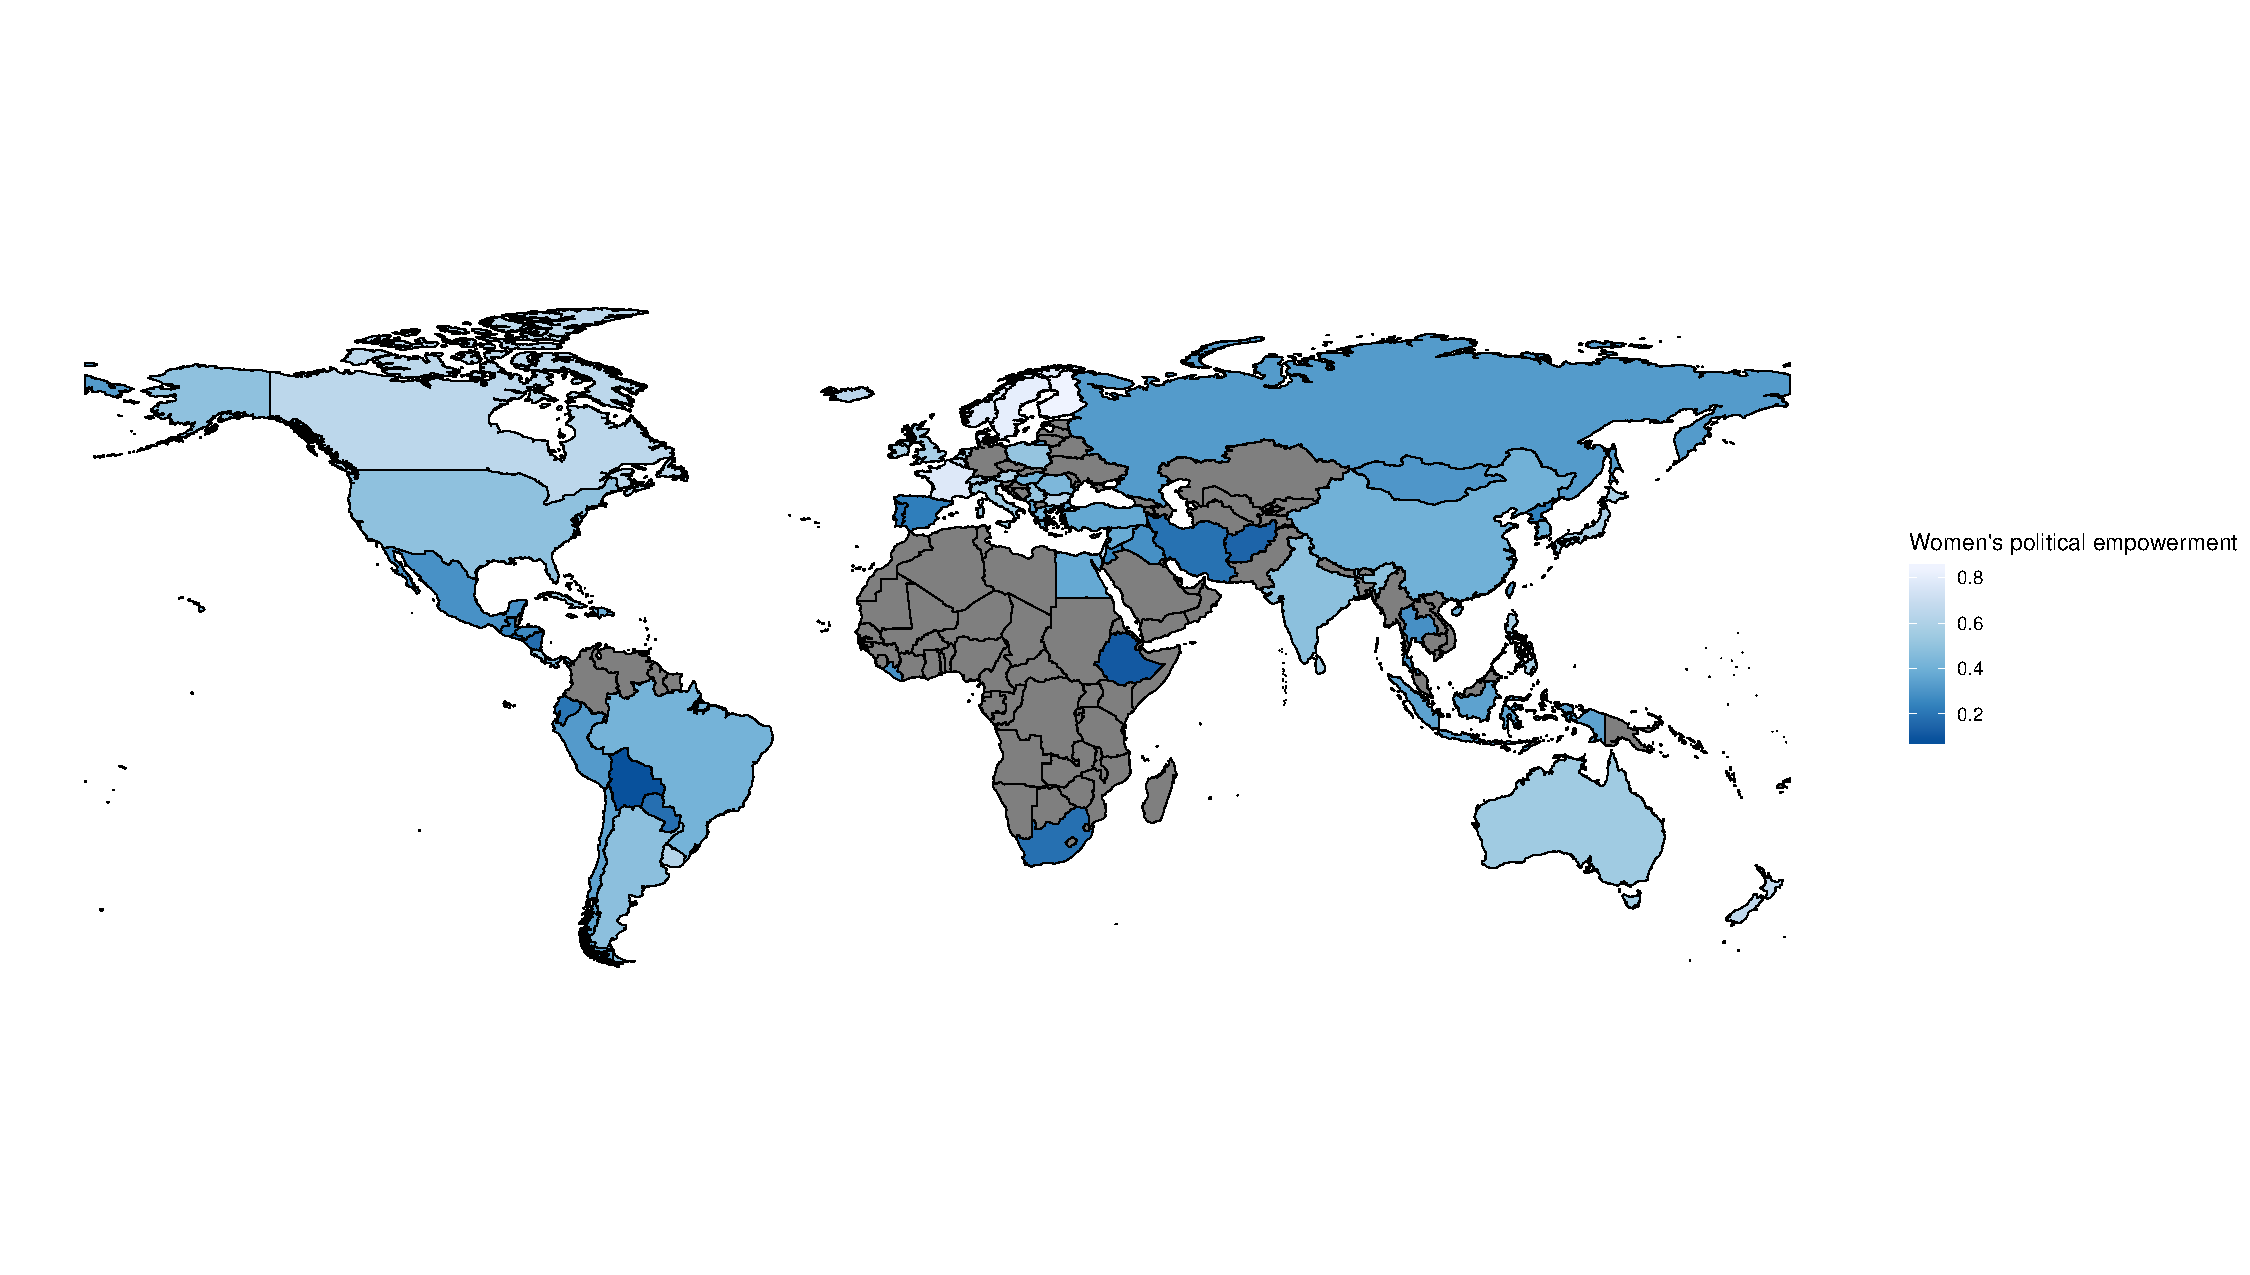
\includegraphics[scale=.2]{Fig1a.pdf}}     
       \subfigure[Women's political empowerment index in 2005]{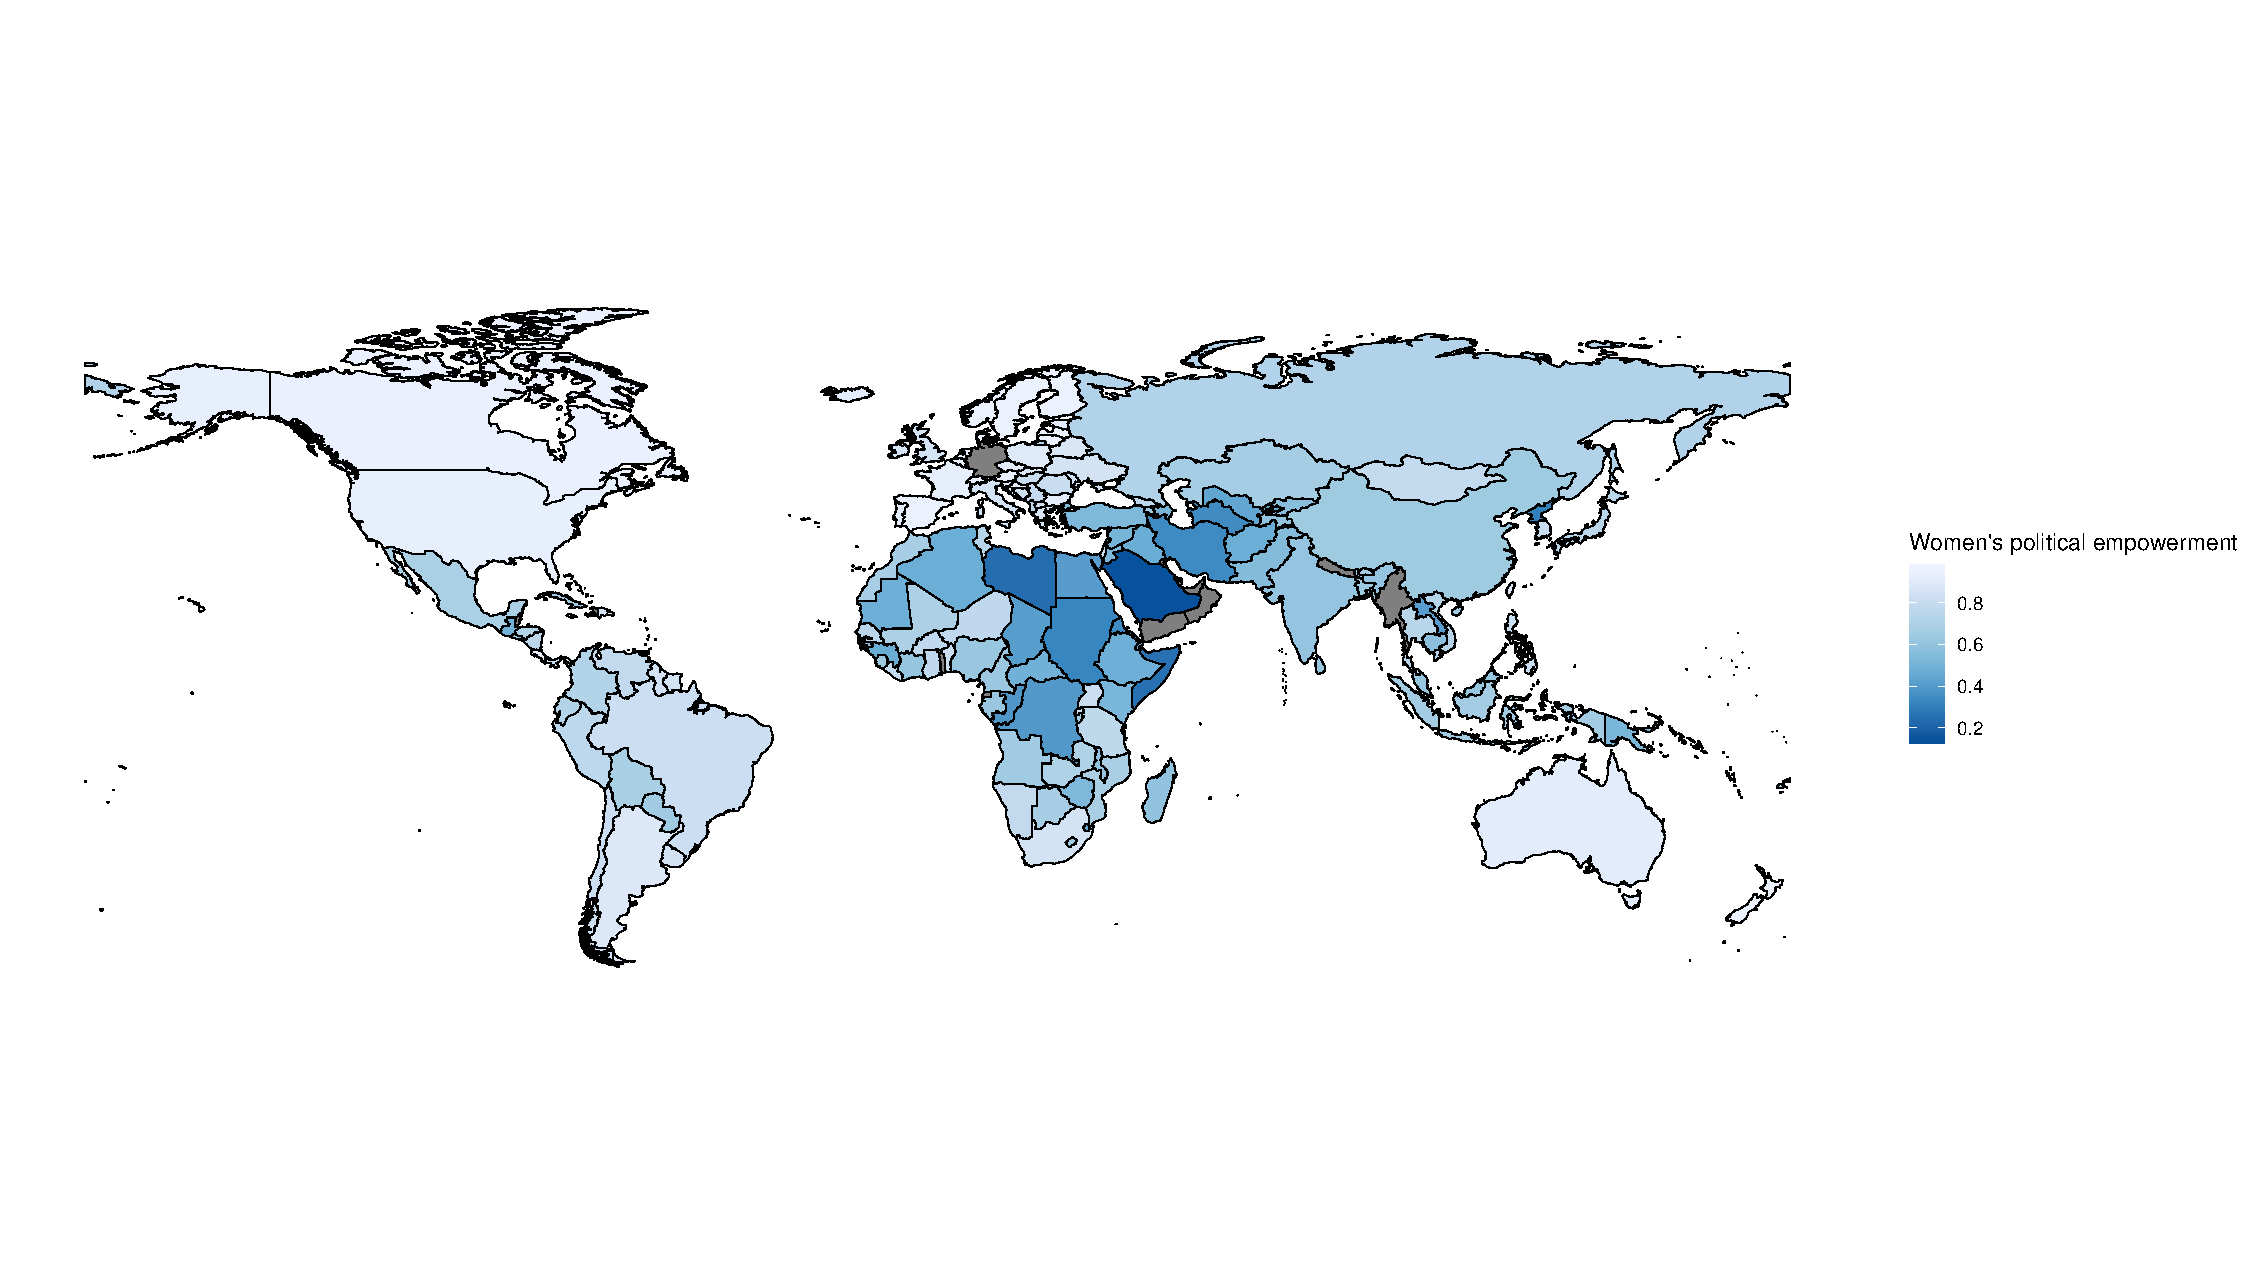
\includegraphics[scale=.2]{Fig1b.pdf}}    
          \subfigure[Women's political empowerment index and war over time ]{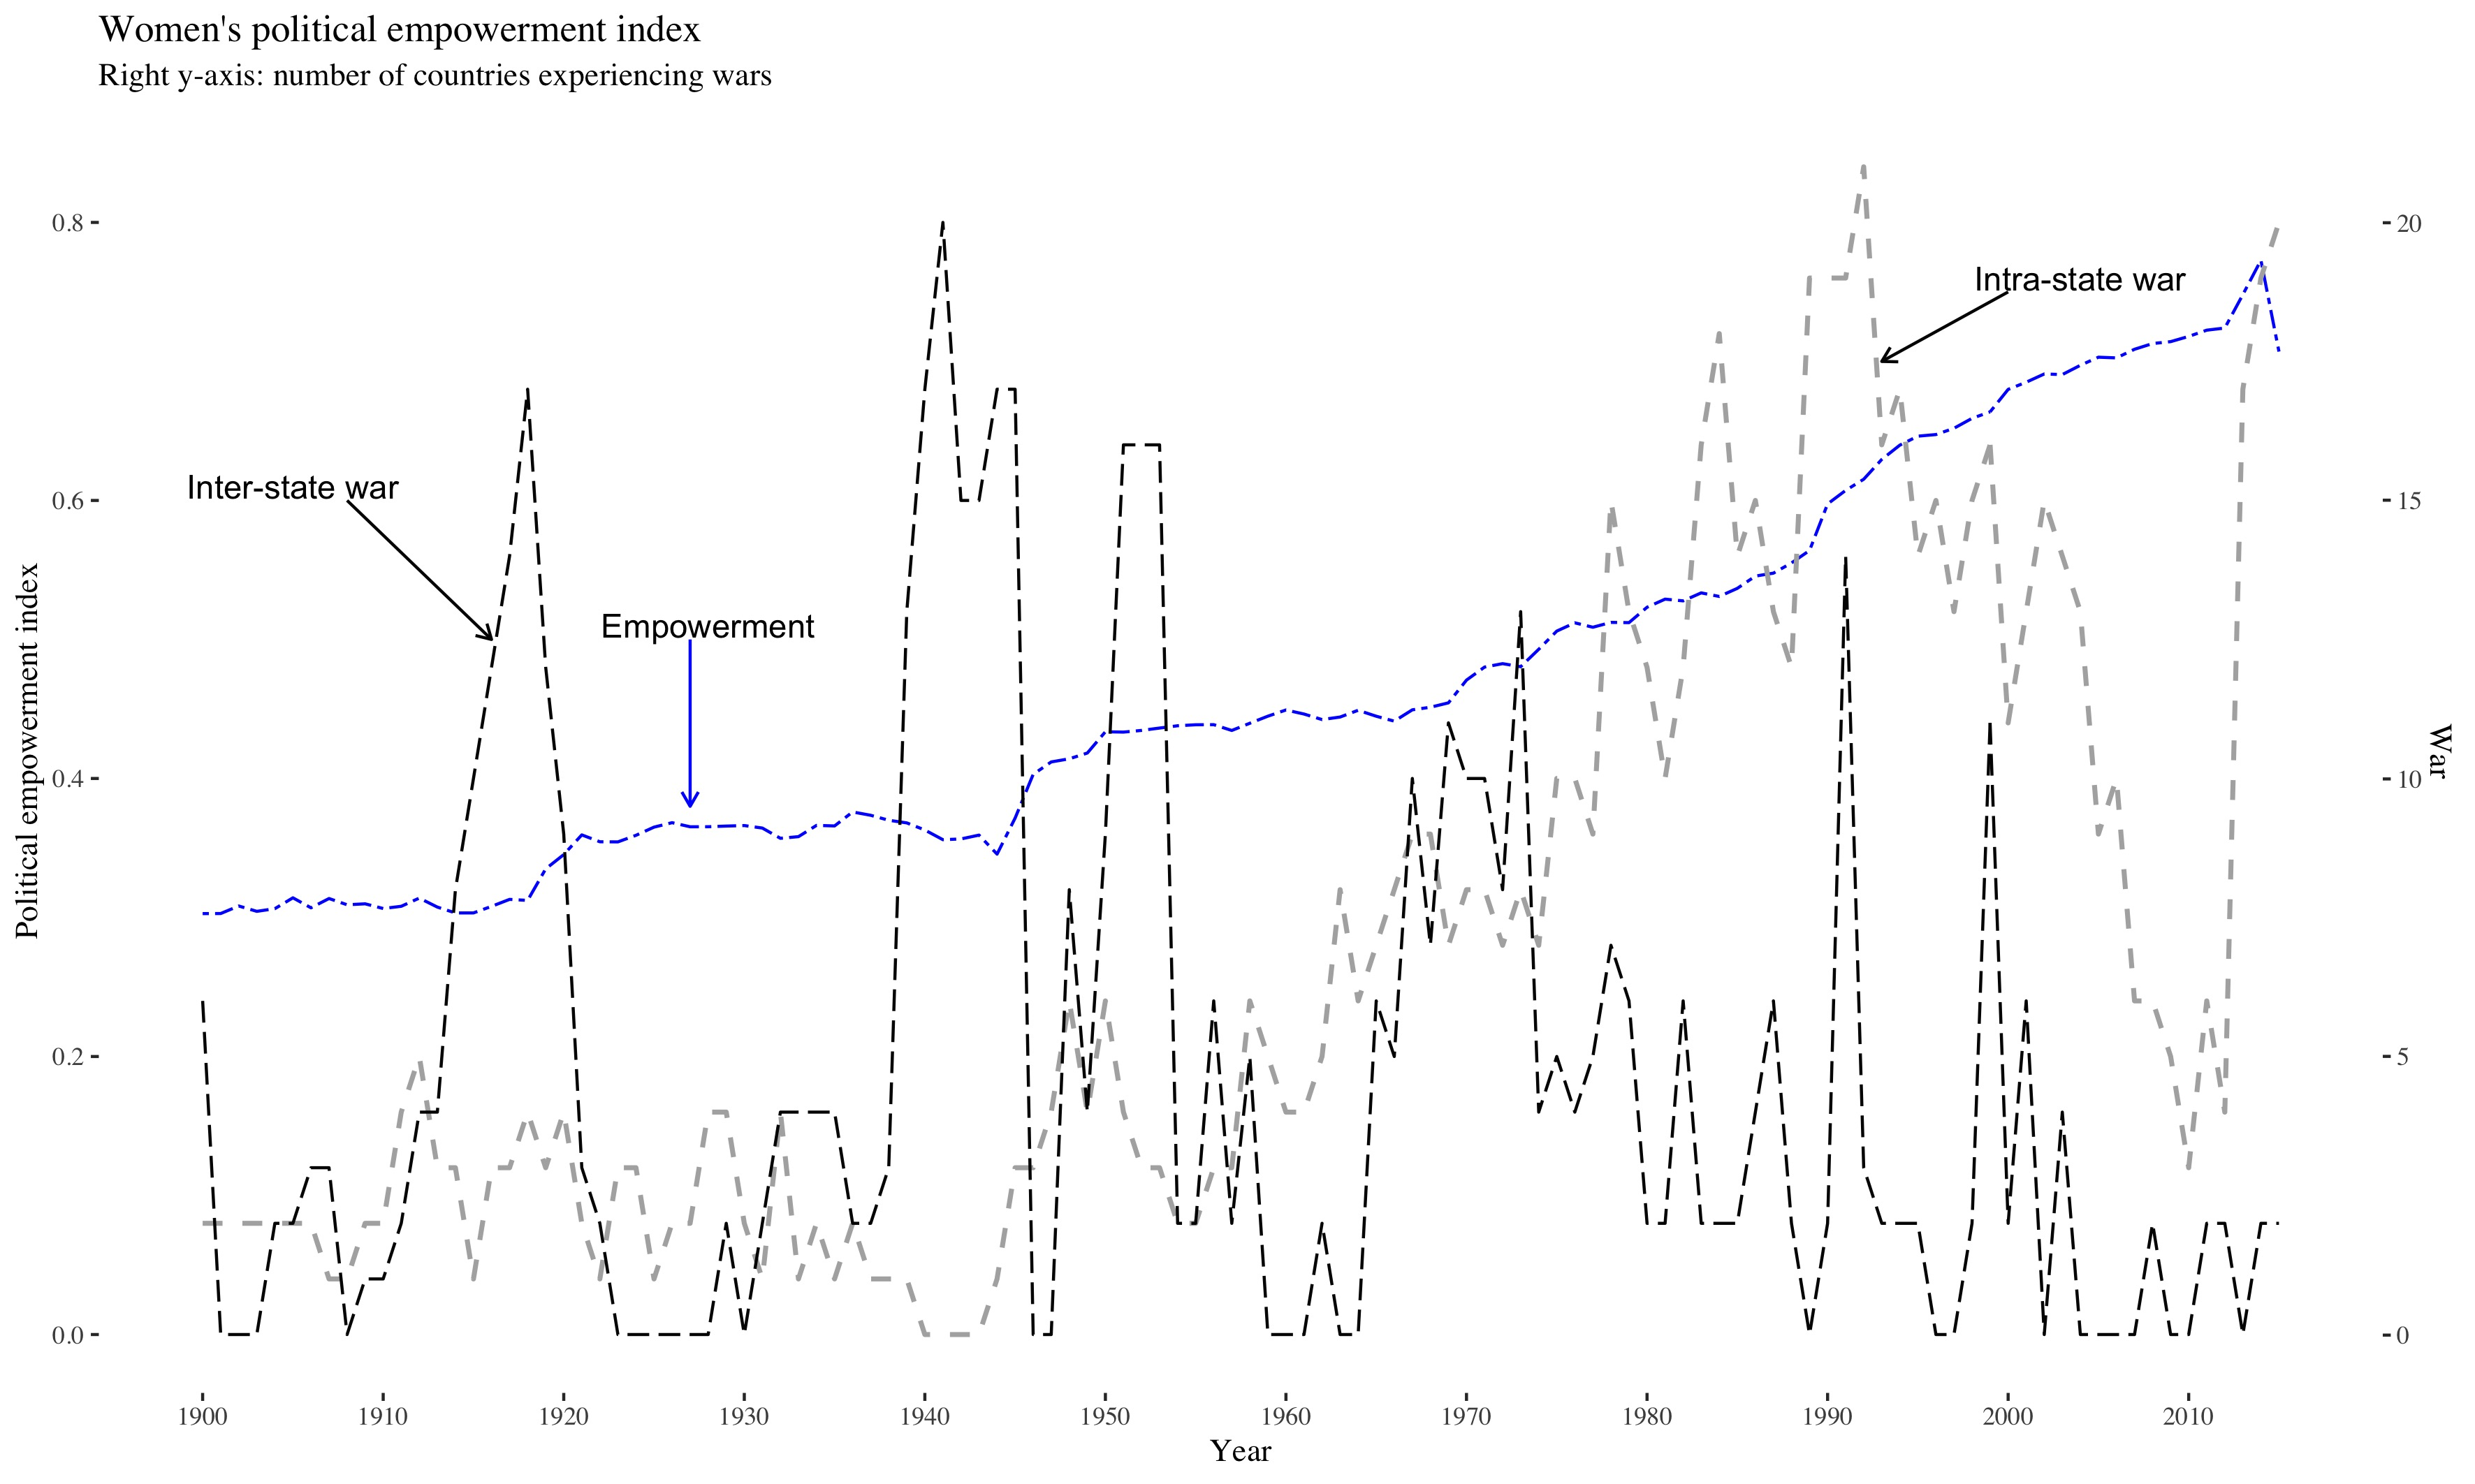
\includegraphics[scale=.14]{Fig1c.jpg}}    
  \begin{flushleft}  
        {\footnotesize {\it Note}: Panels a - b of Figure \ref{dv1} show the geographic distribution of {\it women's political empowerment} in 1950 and 2005. The gray areas denote missing data (e.g., countries have not yet become independent) while the lighter the color, the more women are empowered. Panel c of  Figure \ref{dv1} displays the global average trend of women's political empowerment (left y-axis)  from 1900 to 2015 along with the number of countries experiencing different types of wars (right y-axis).}
       \end{flushleft} 
\end{figure}


% Figure 2
\begin{figure}[h]
   \centering
    \caption{Women's Empowerment for Select Countries, 1900-2015 }
    \label{dv2}
  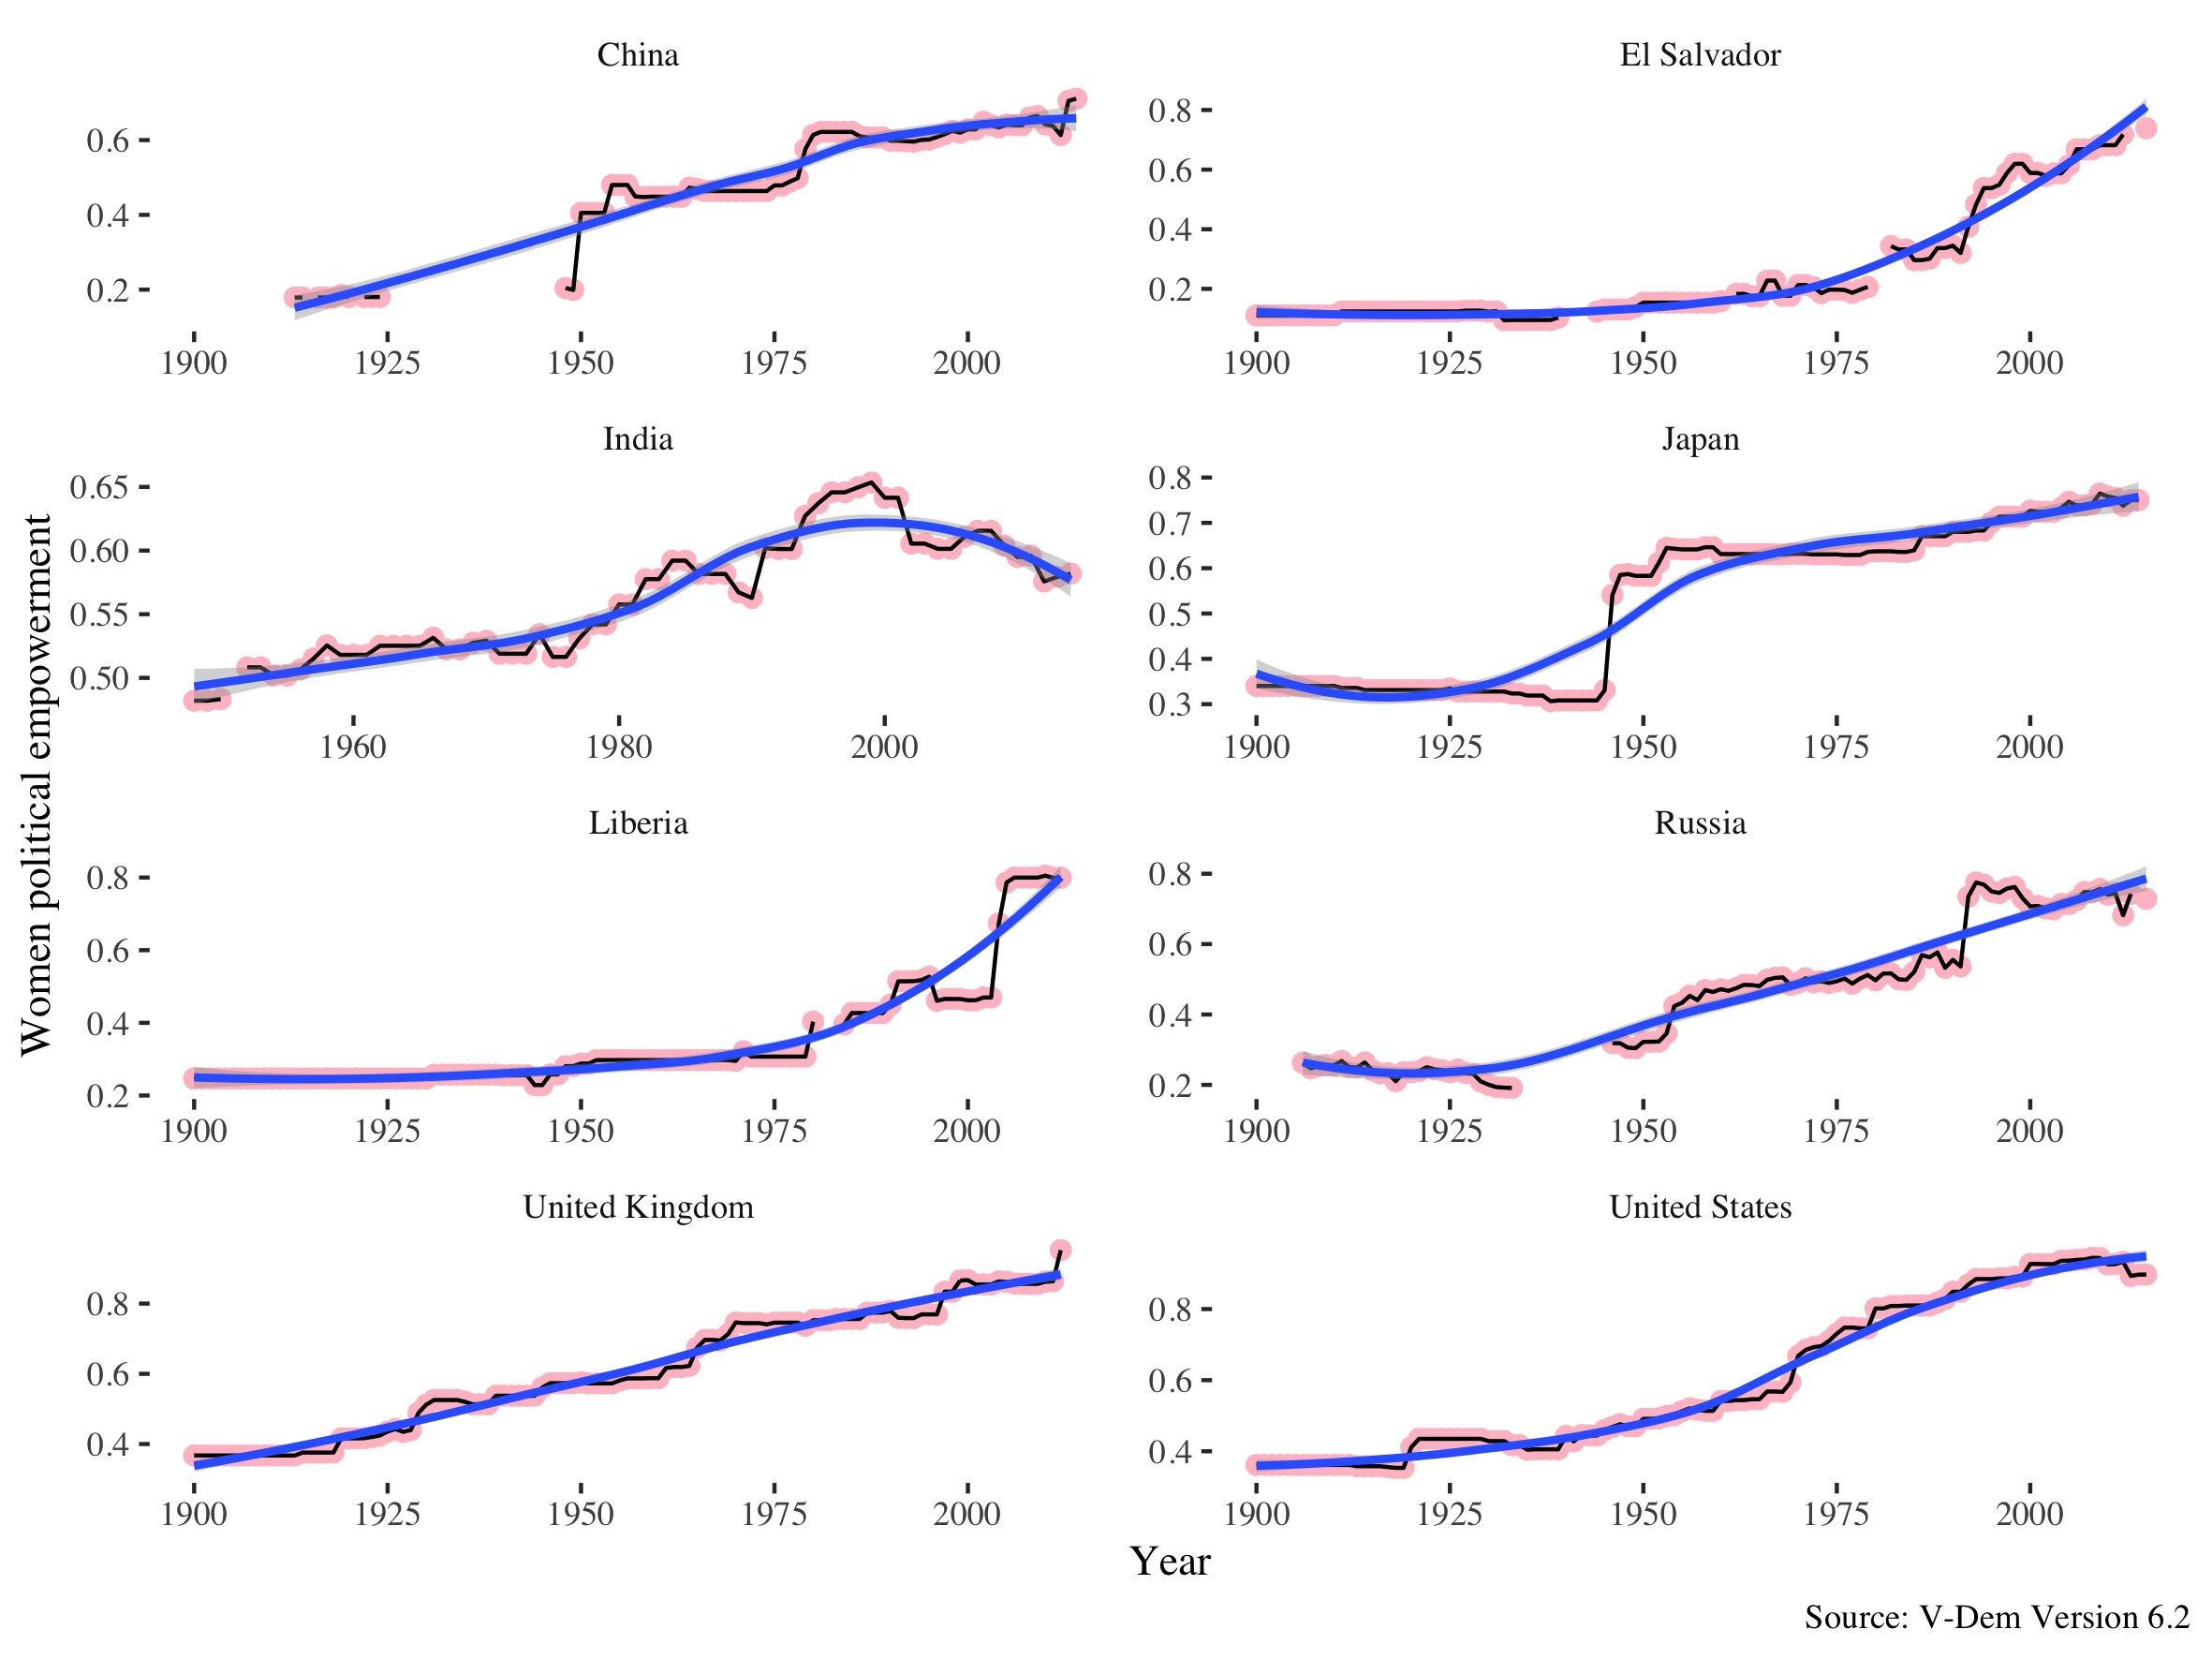
\includegraphics[scale=.2]{Fig2.jpg}
  \begin{flushleft}  
        {\footnotesize {\it Note}: Figure \ref{dv2} shows the evolution of the {\it women's political empowerment index} for China, El Salvador, India, Japan, Liberia,  Russia, United Kingdom, and United States from 1900 to 2015. The blue lines fit a loess-smoothing function and the discontinuities denote missing data.}
       \end{flushleft} 
\end{figure}

% Figure 3 
\begin{figure}[h]
   \centering
    \caption{Marginal Forward Effects of War on Women's Political Empowerment}
    \label{war}
  \subfigure[Forward effects of war]{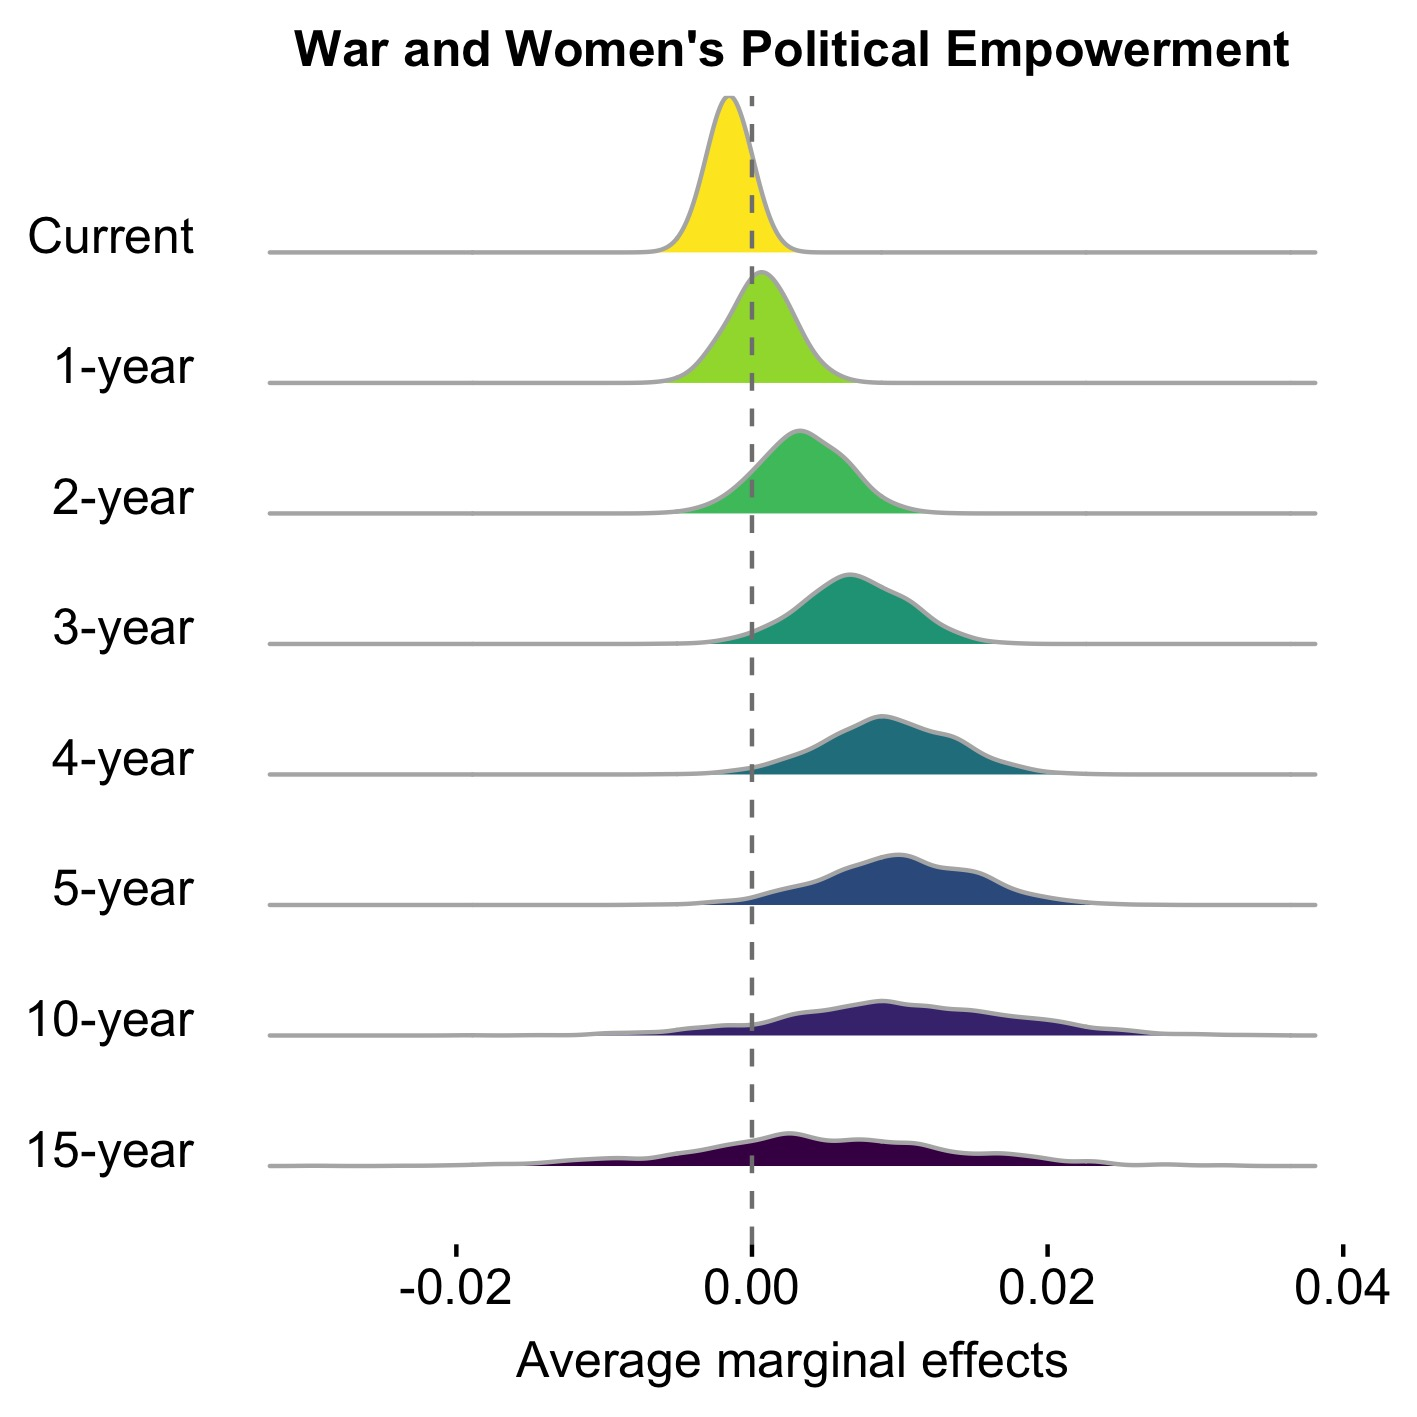
\includegraphics[scale=.15]{Fig3.jpg}}
    \subfigure[Forward effects of new war]{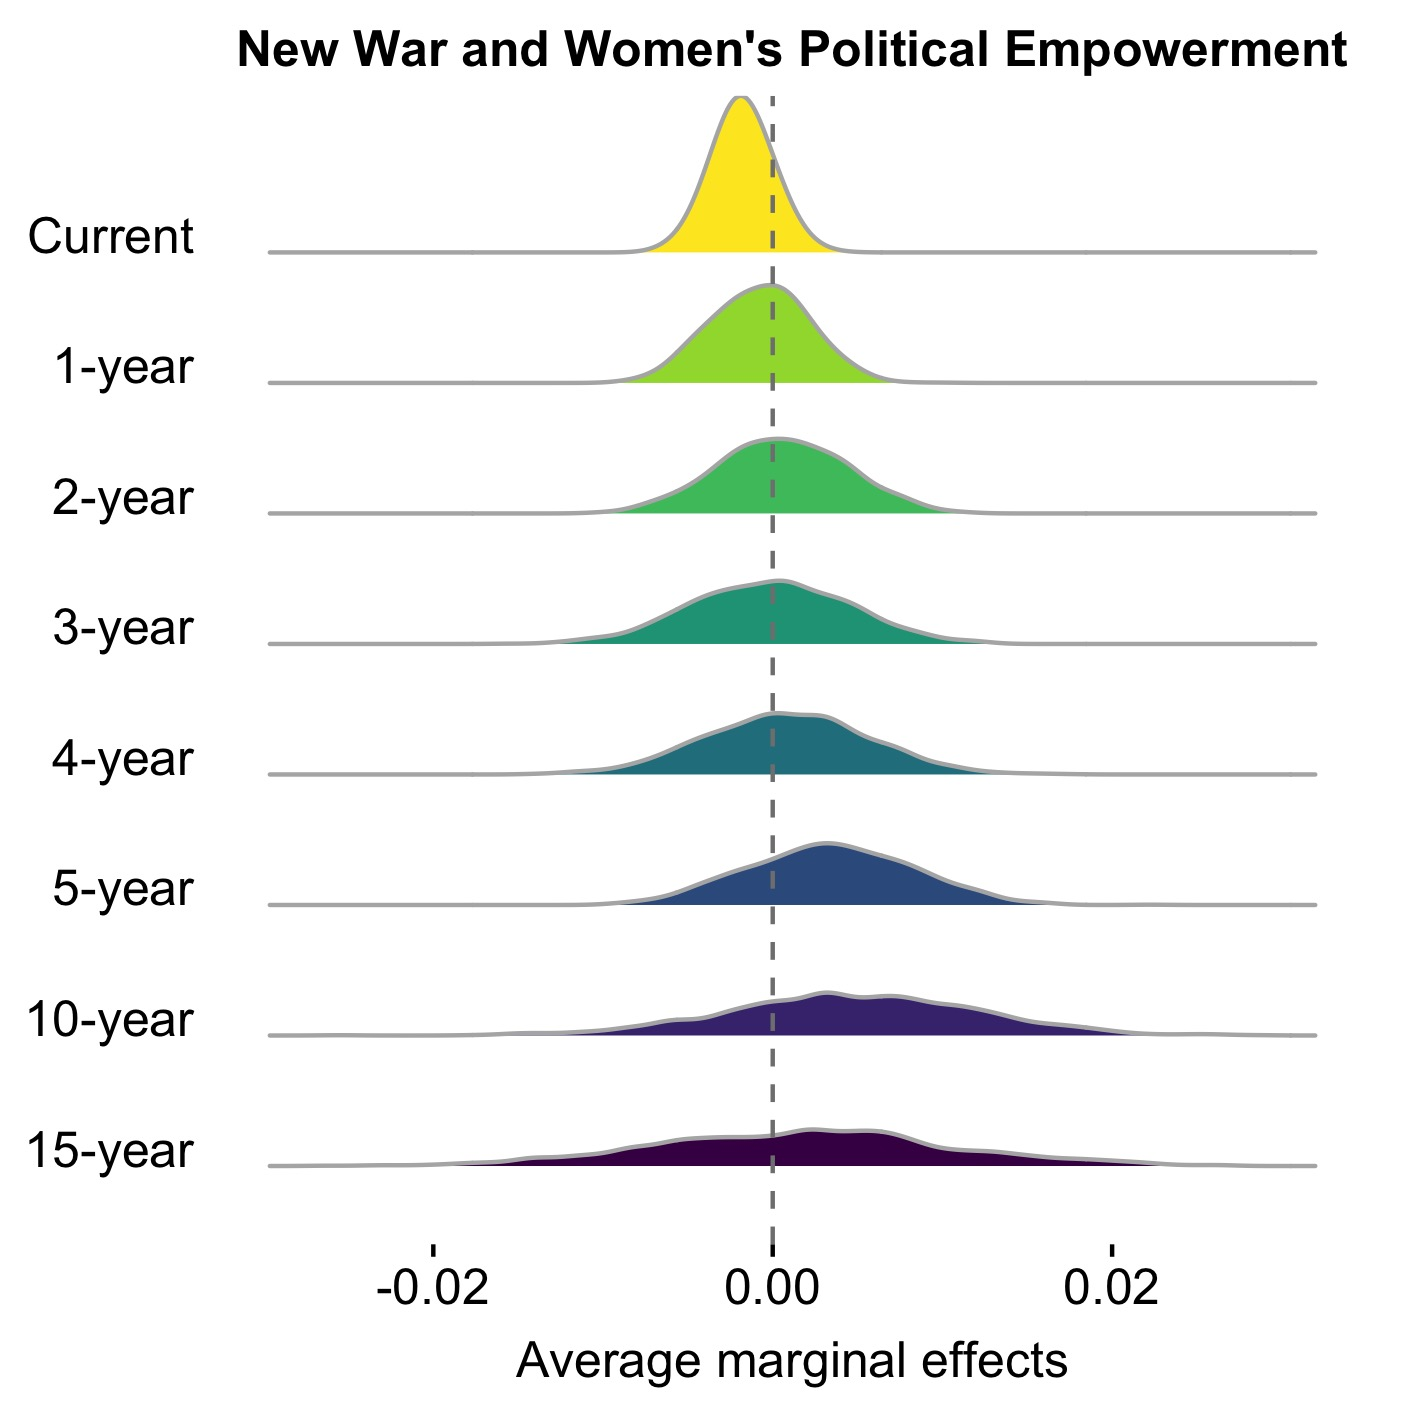
\includegraphics[scale=.15]{Fig3_newwar.jpg}}
    \subfigure[Forward effects of ongoing war]{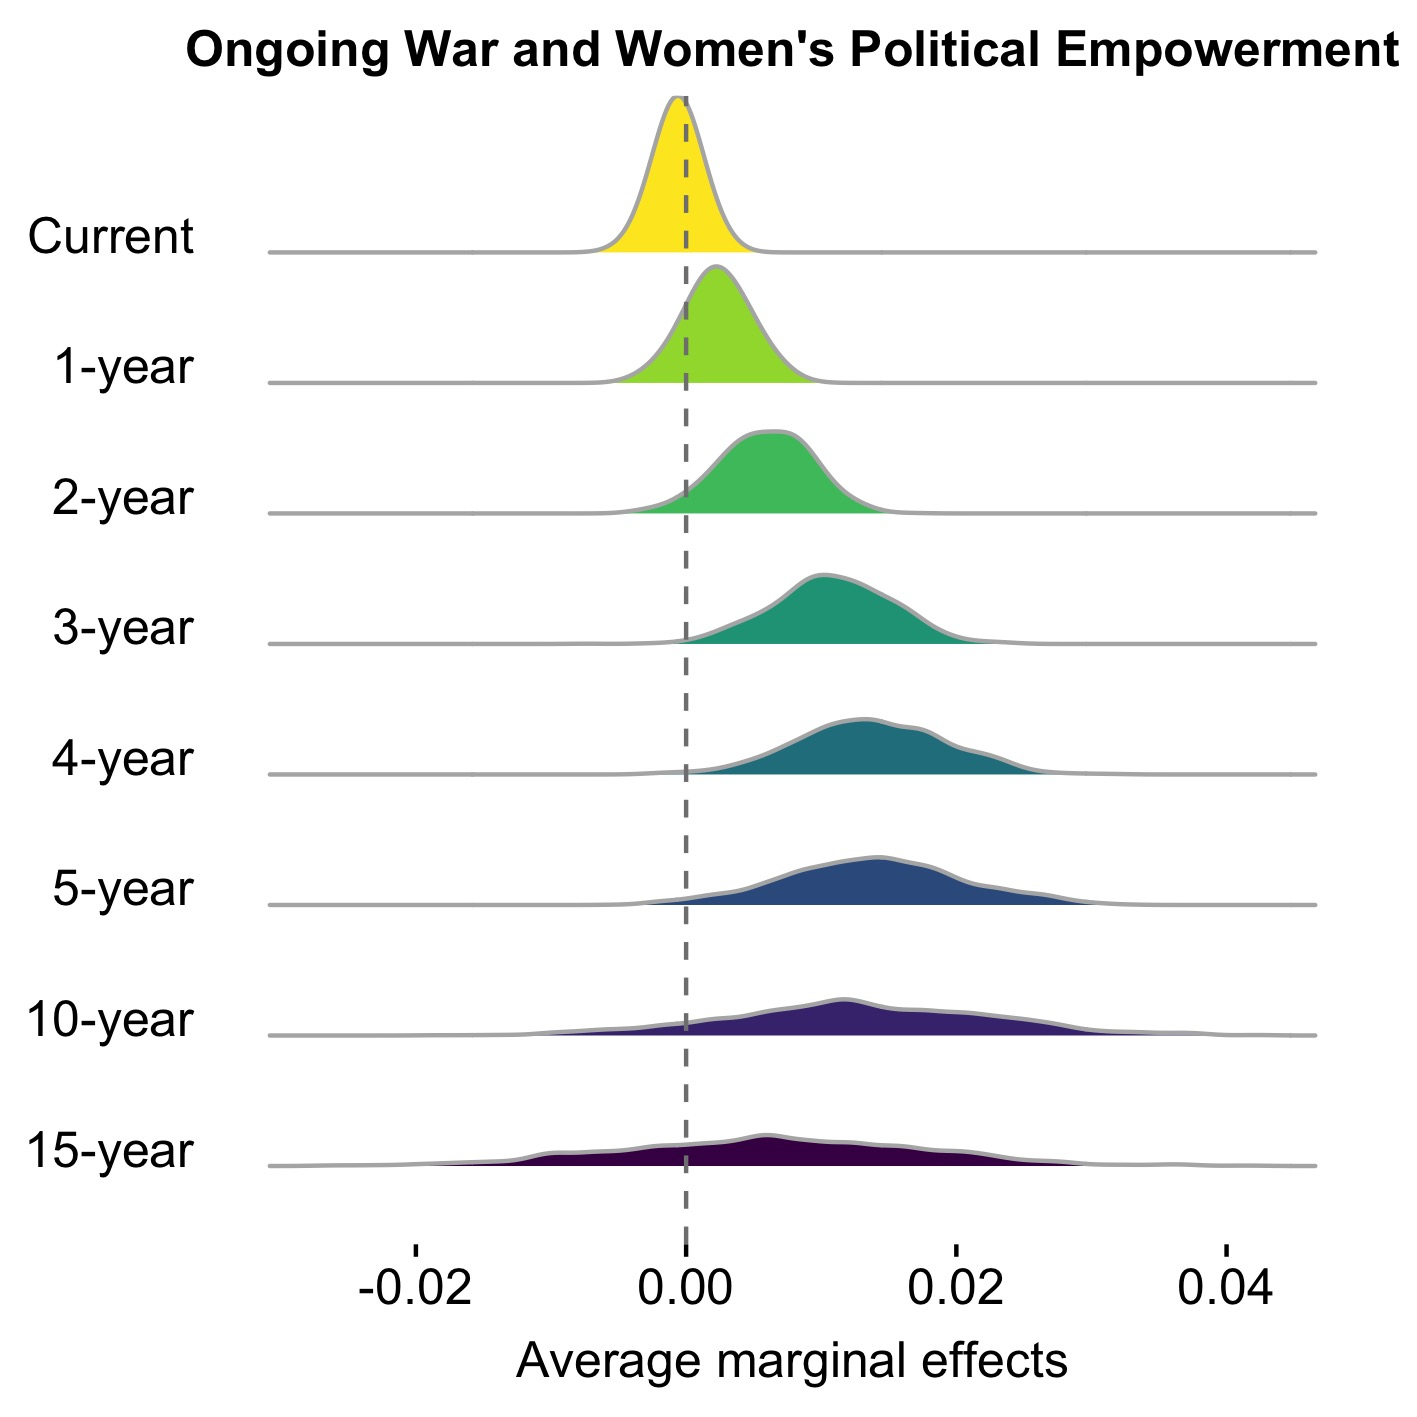
\includegraphics[scale=.15]{Fig3_ongoingwar.jpg}}
    \subfigure[Forward effects of recent war]{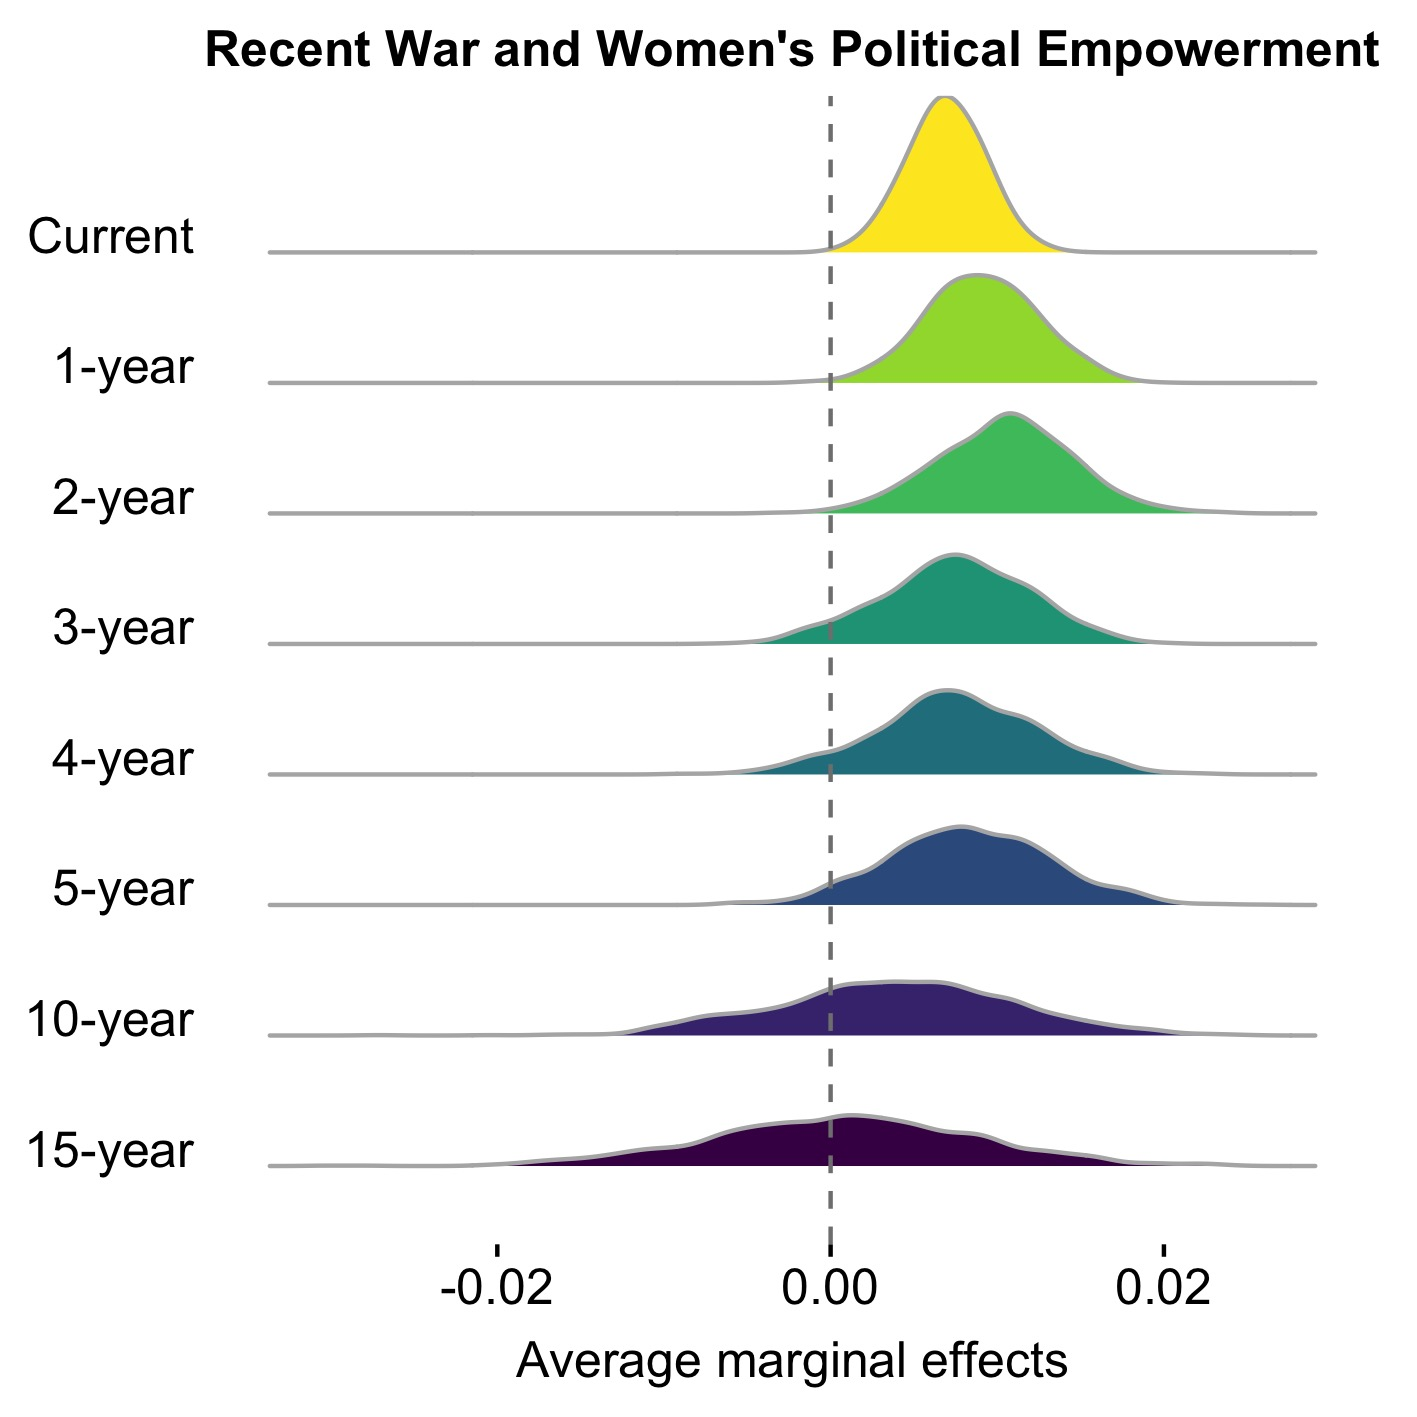
\includegraphics[scale=.15]{Fig3_recentwar.jpg}}
  \begin{flushleft}  
        {\footnotesize {\it Note}: Panel a of Figure \ref{war} shows the distributions of the predicted marginal forward effects of war, based on the variable {\it war} %across the Models 1-8
  in Table \ref{tab2}. Panels b through d  shows the distributions of the predicted marginal forward effects of periods of new war, ongoing war and recent war, based on the different treatment variables %across Models 9-16
  in Table \ref{tab3}. }
       \end{flushleft} 
\end{figure}

% Figure 4
\begin{figure}[h]
   \centering
    \caption{Marginal Forward Effects of War on Women's Political Empowerment, IV Model}
    \label{IV}
	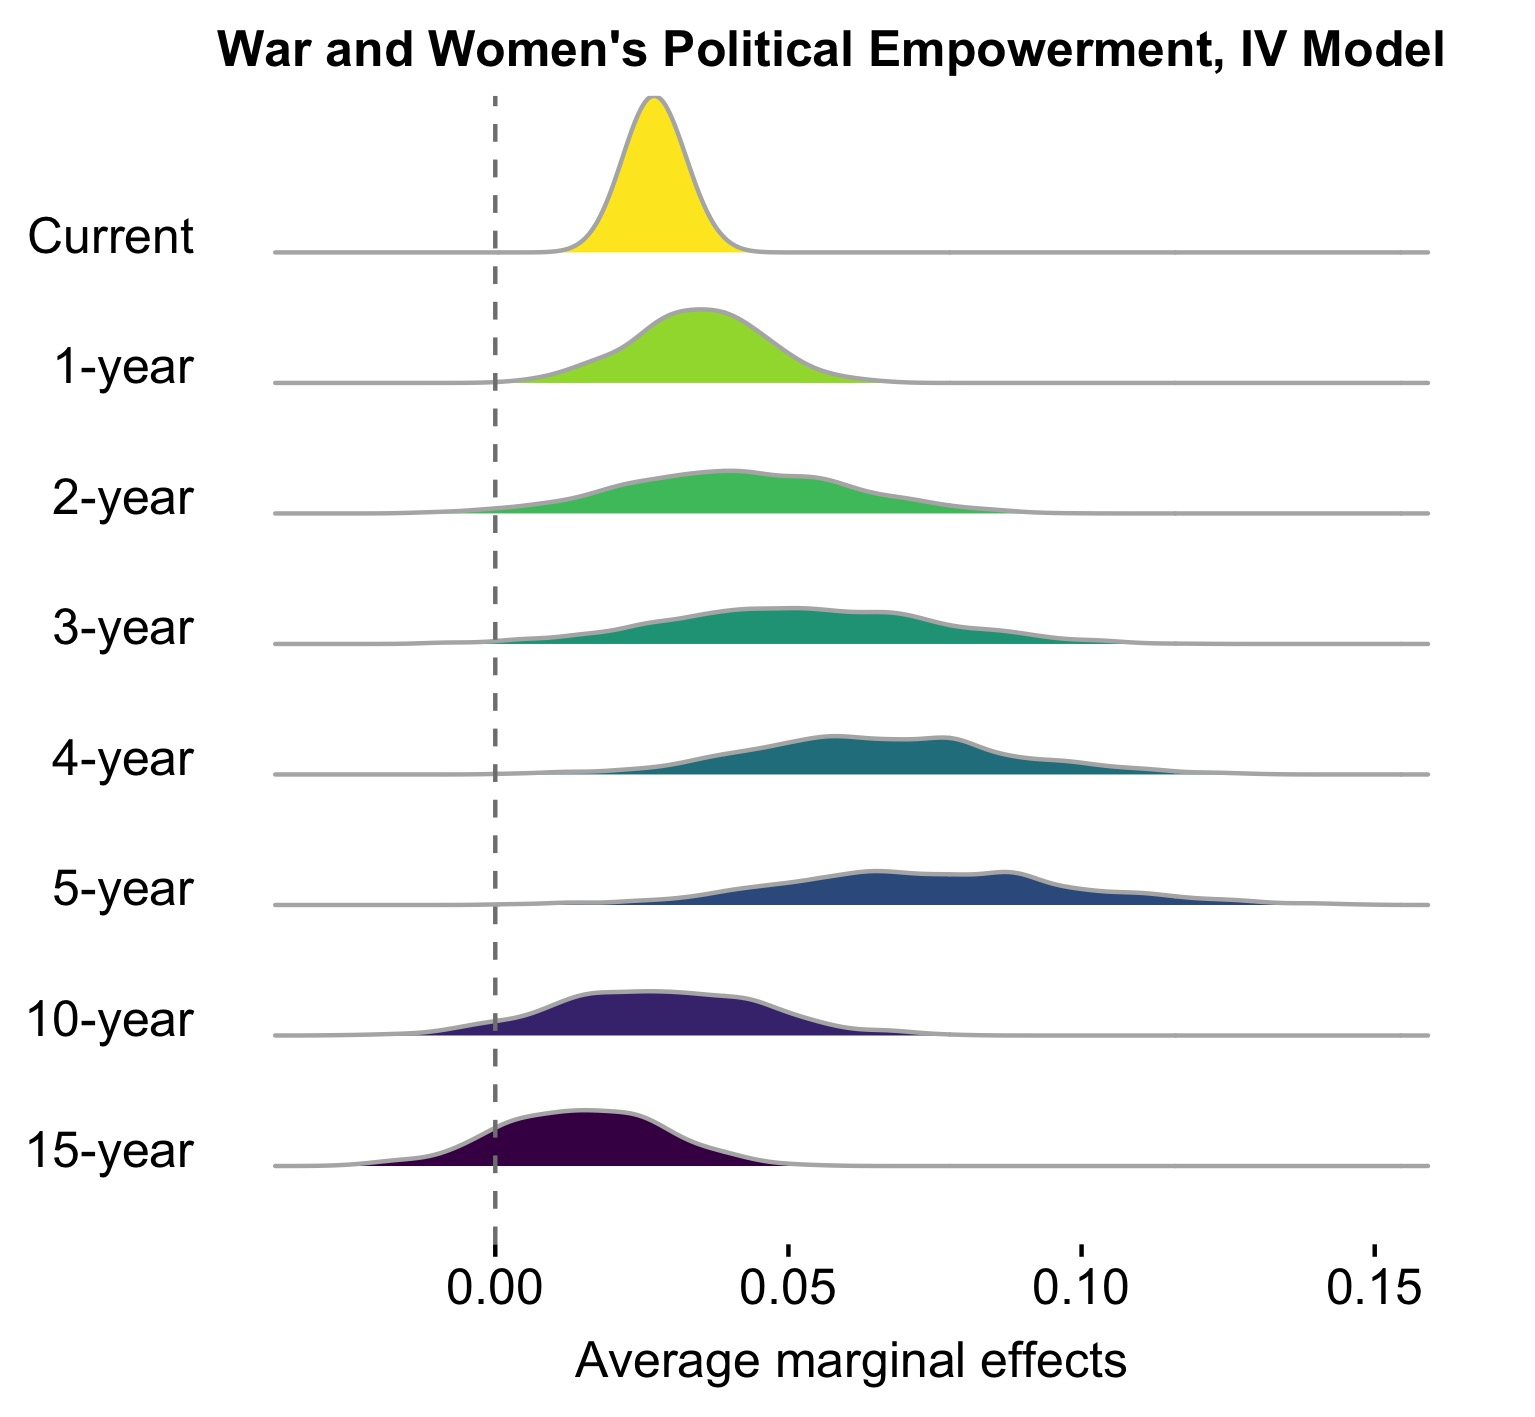
\includegraphics[scale=.15]{Fig4.jpg}
  \begin{flushleft}  
        {\footnotesize {\it Note}: Figure \ref{IV} shows the distributions of the predicted marginal forward effects of war from an endogenous treatment regressions model. The density plots are based on the treatment variable in the outcome stage %across Models 17-24
 in Table \ref{ivpolempowerment}. }
       \end{flushleft} 
\end{figure}

%Figure 5
\begin{figure}[h]
   \centering
    \caption{Marginal Forward Effects of War Duration and Battle Deaths on Women's Political Empowerment}
    \label{durbd}
  \subfigure[Forward effects of war duration]{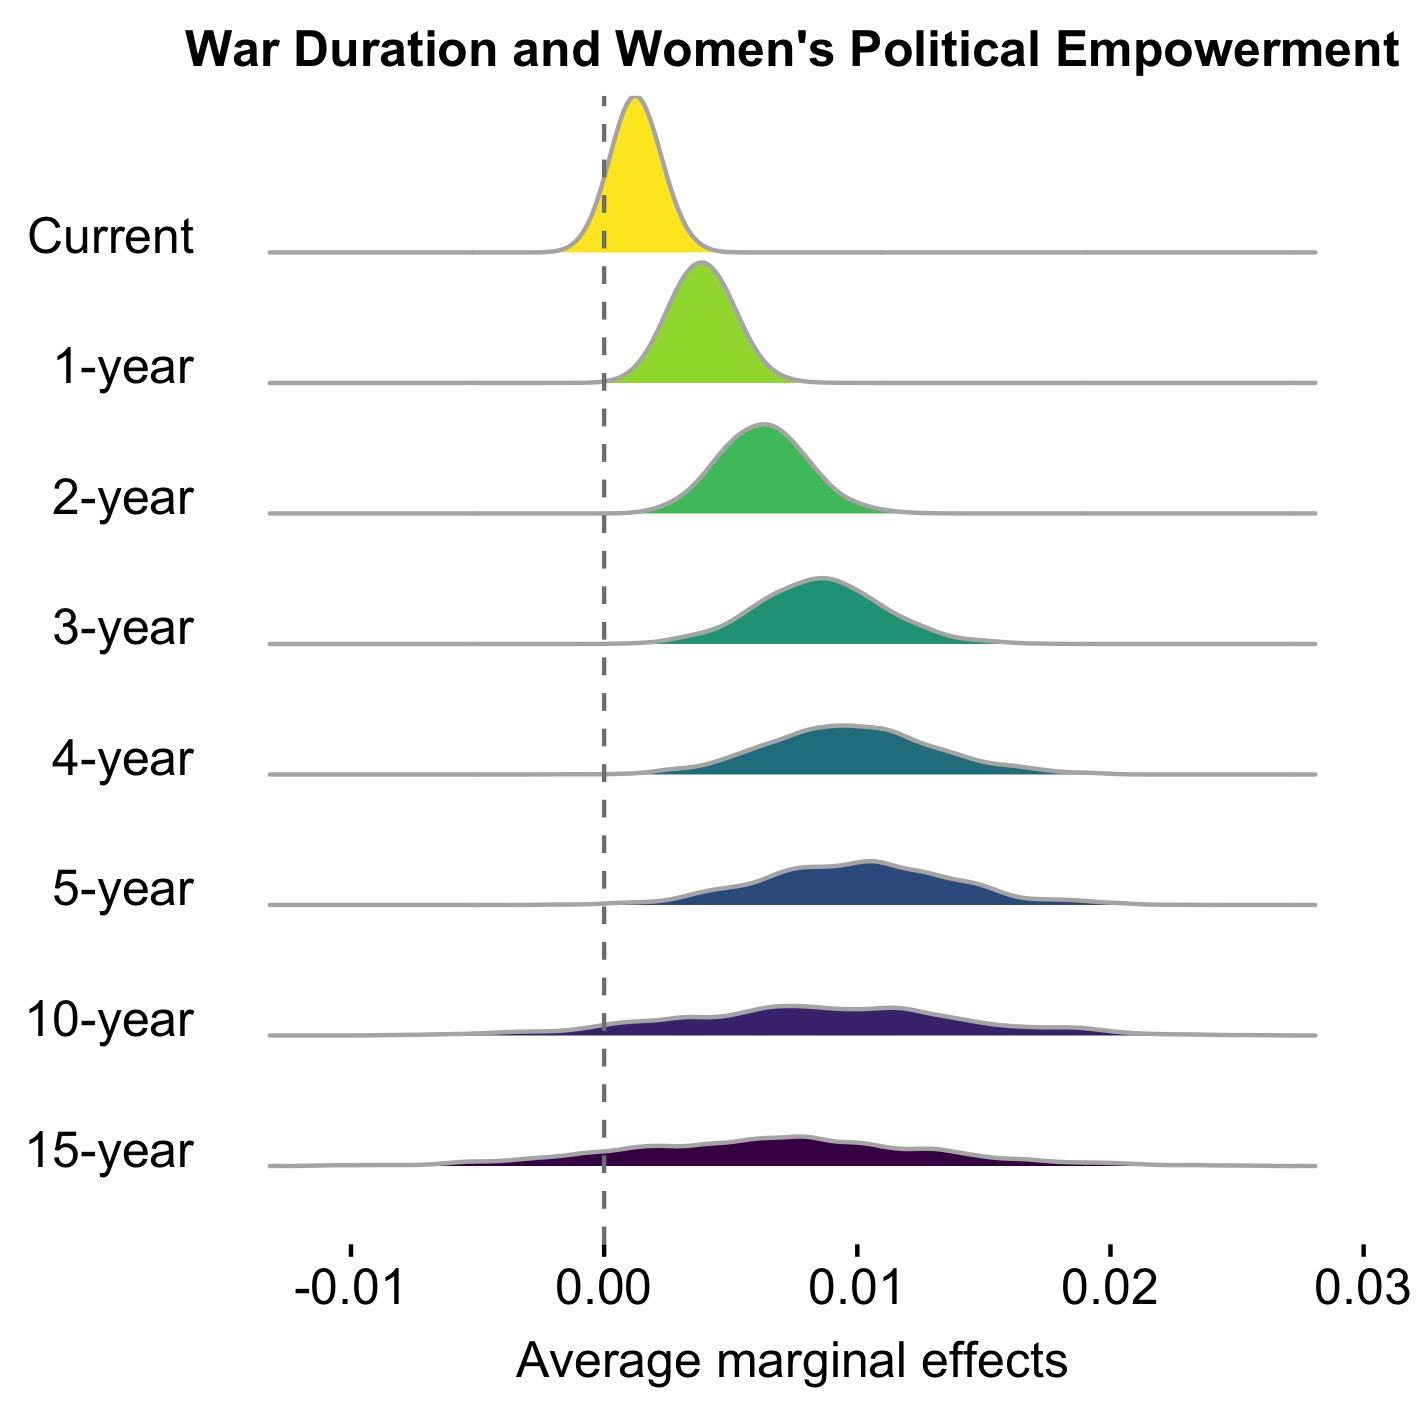
\includegraphics[scale=.15]{Fig5-a.jpg}}
    \subfigure[Forward effects of battle deaths (logged)]{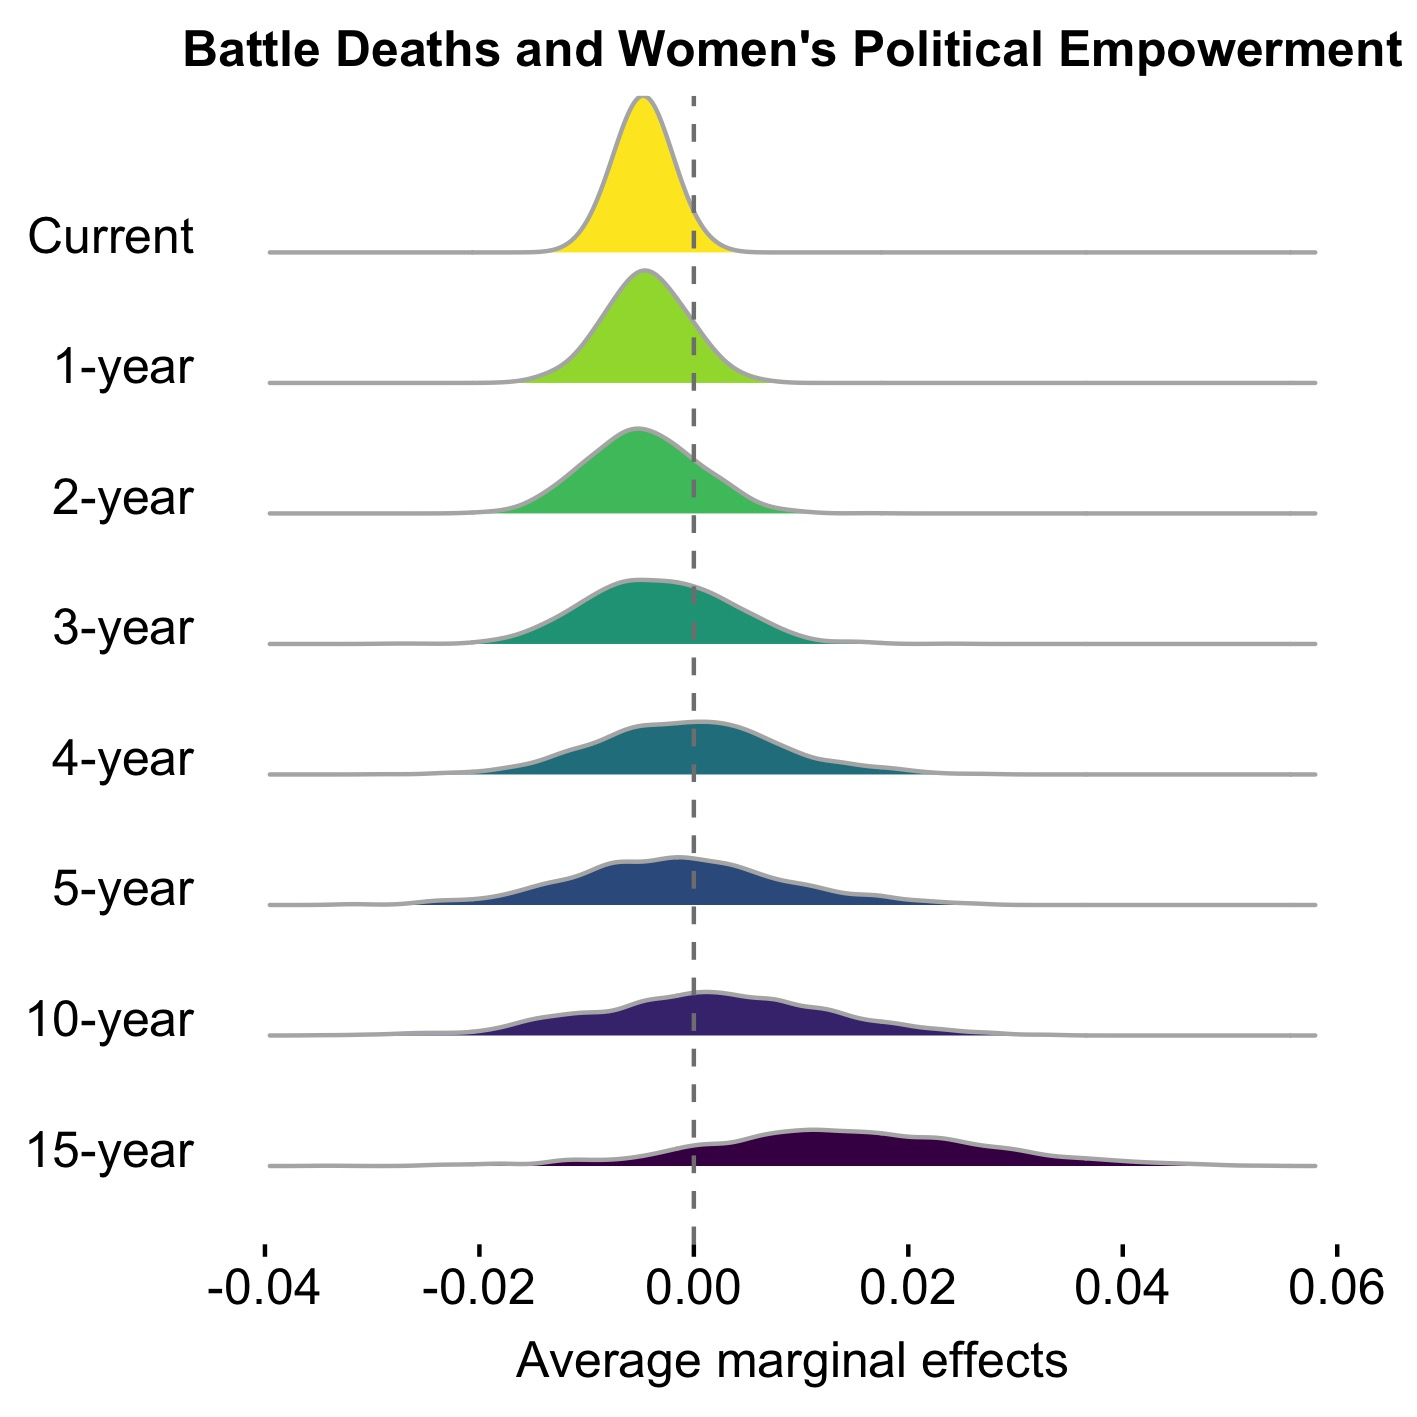
\includegraphics[scale=.15]{Fig5-b.jpg}}
  \begin{flushleft}  
        {\footnotesize {\it Note}: Figure \ref{durbd} shows the distributions of the predicted marginal forward effects of war duration and battle-related fatalities. The density plots in panel a are based on the variable {\it war duration} changing from 0 to 5 (i.e., 2.5\% quantile to 97.5\% quantile) %across the Models 25-32 
 in Table \ref{polwardur}. The density plots in panel b are based on the variable {\it log of battle deaths} changing from 0 to 8.9 (i.e., 2.5\% quantile to 97.5\% quantile) %across the Models 33-40 
 in Table \ref{polbdeath}.}
       \end{flushleft} 
\end{figure}

%Figure 6
\begin{figure}[h]
   \centering
    \caption{Marginal Forward Effects of War on Changing Fertility Rates}
    \label{fig:fertility}
 \subfigure[Forward effects of war]{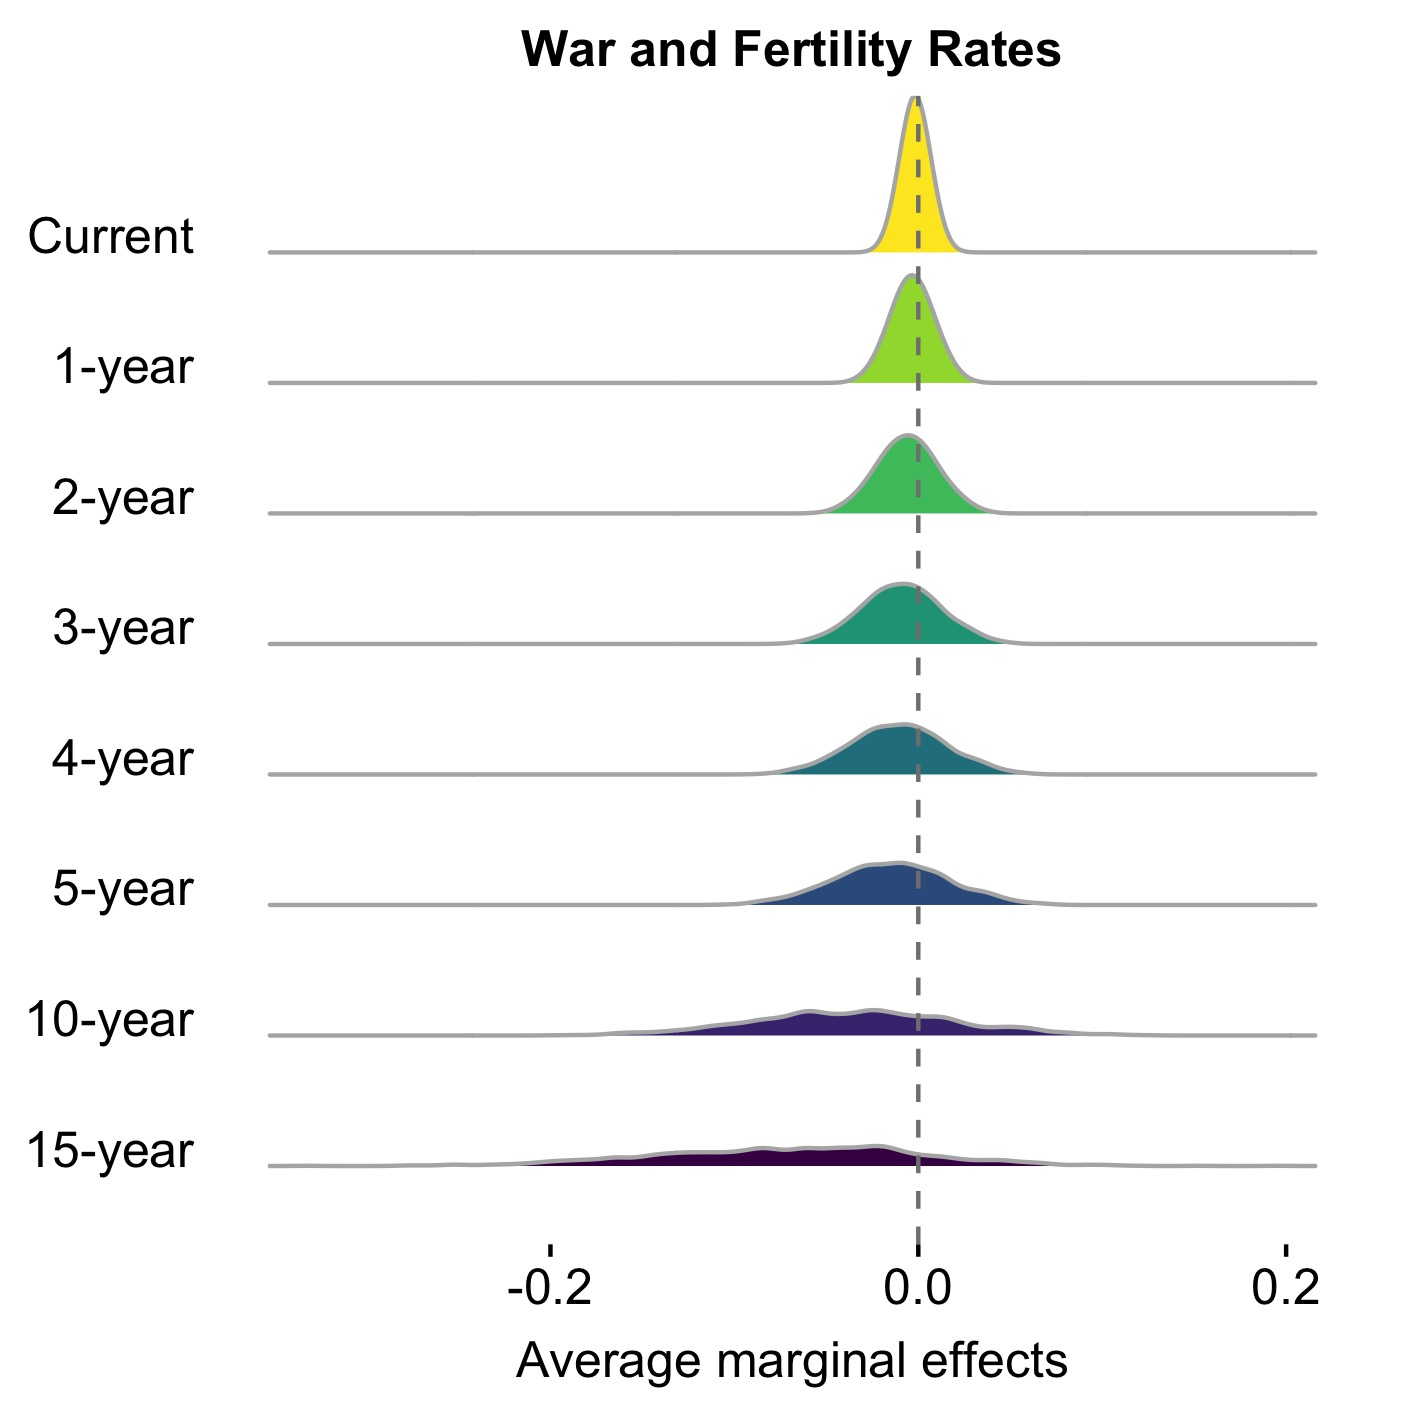
\includegraphics[scale=.15]{Fig6-a.jpg}}
    \subfigure[Forward effects of existential war]{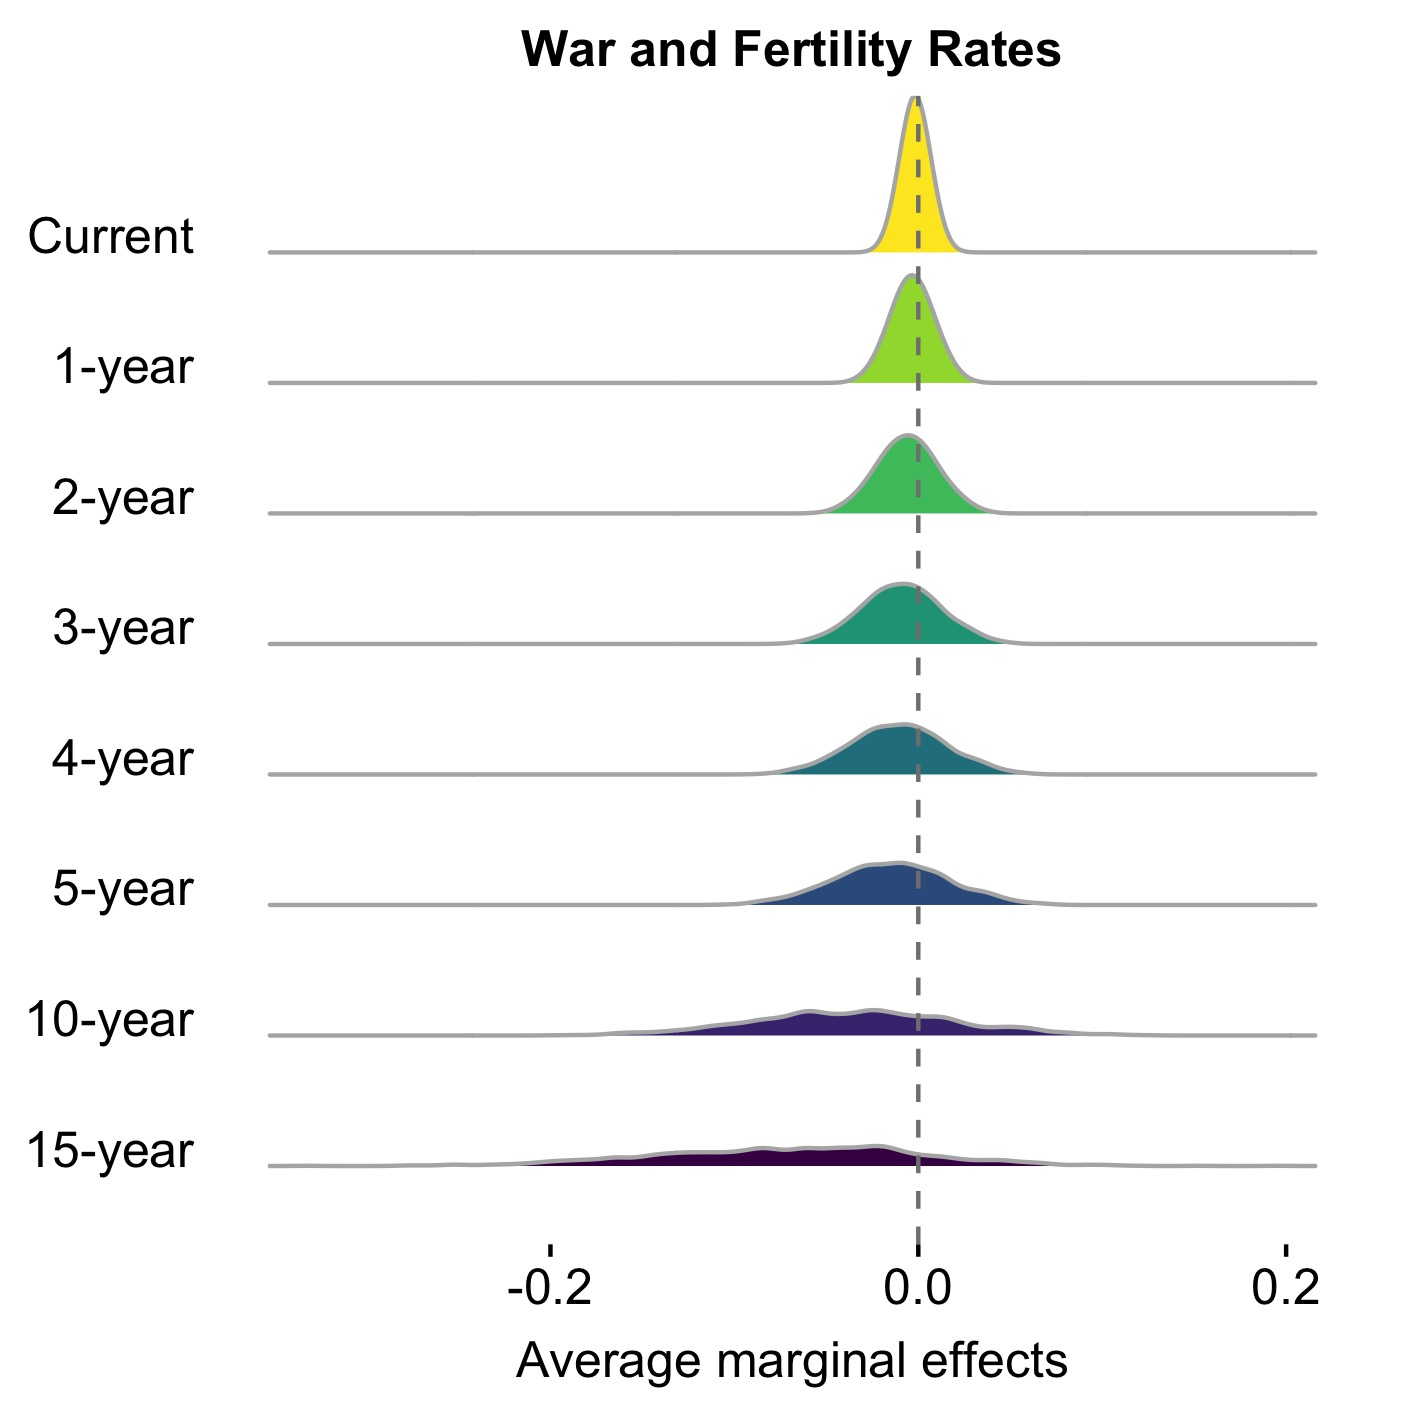
\includegraphics[scale=.15]{Fig6-a.jpg}}
  \begin{flushleft}  
        {\footnotesize {\it Note}: Figure \ref{fig:fertility} shows the effects of war and existential war on changes in women's fertility rates. The density plots in panel a are based on the variable {\it war} in Table \ref{fefertility}. The density plots in panel a are based on the variable {\it existential war} in Table \ref{fefertilityexistential}.}
       \end{flushleft} 
\end{figure}

%Figure 7
\begin{figure}[h]
   \centering
    \caption{The Effect of War via Intermediate Variables}
    \label{fig:intermed}
  \subfigure[The marginal effects of war on intermediate variables]{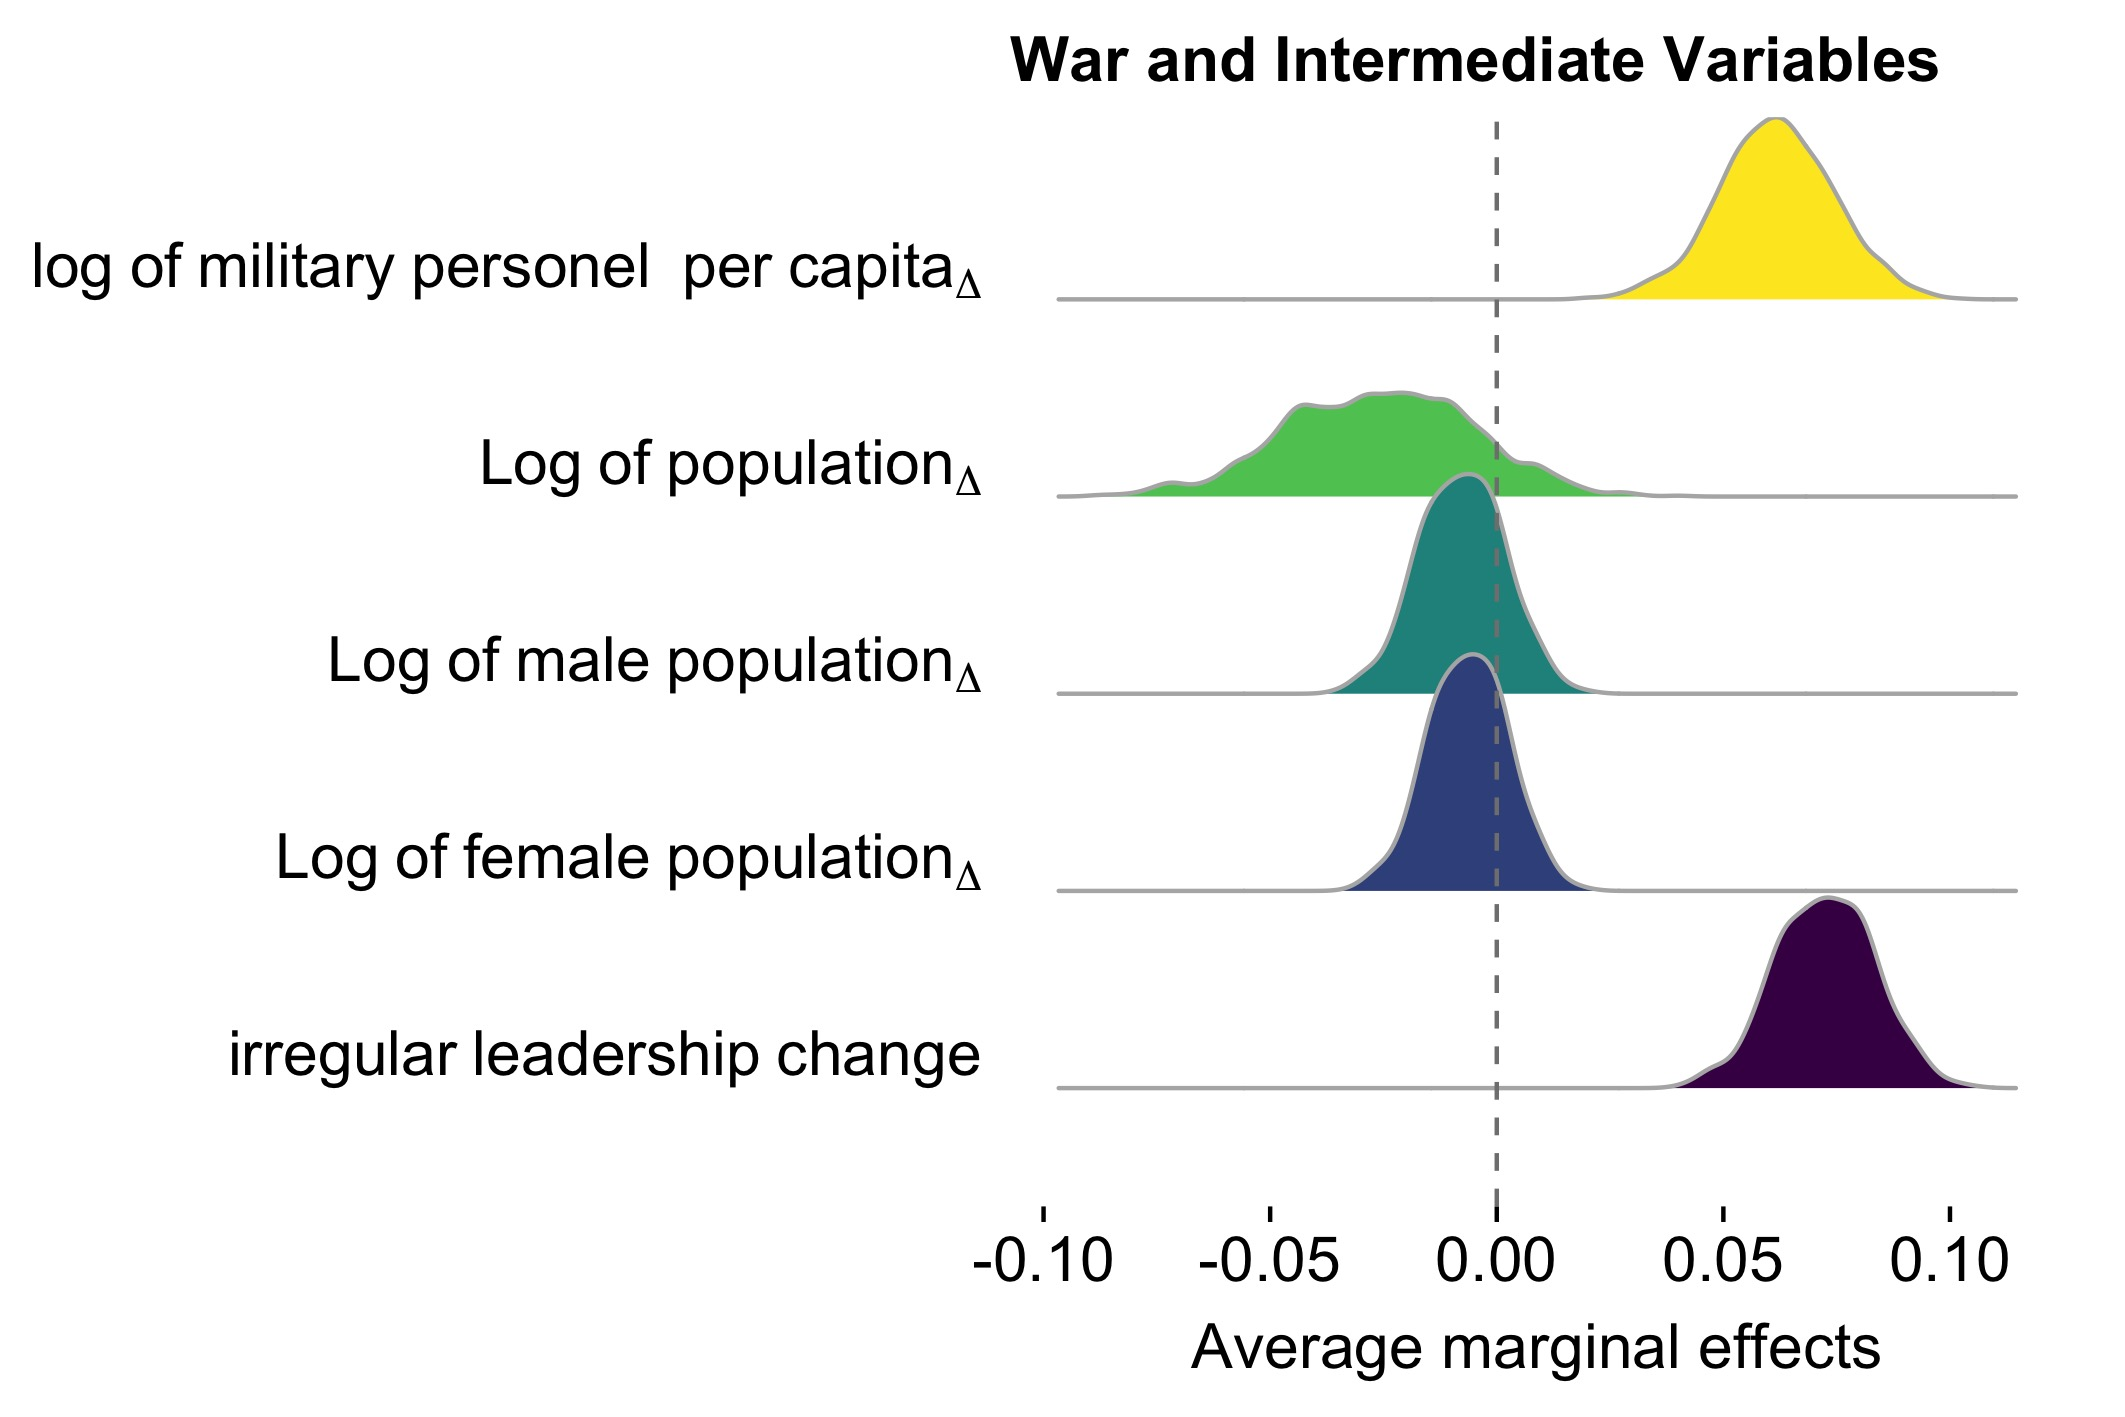
\includegraphics[scale=.1]{Fig7-a.jpg}}
   \subfigure[The marginal forward effects of changes in military personnel on women's empowerment]{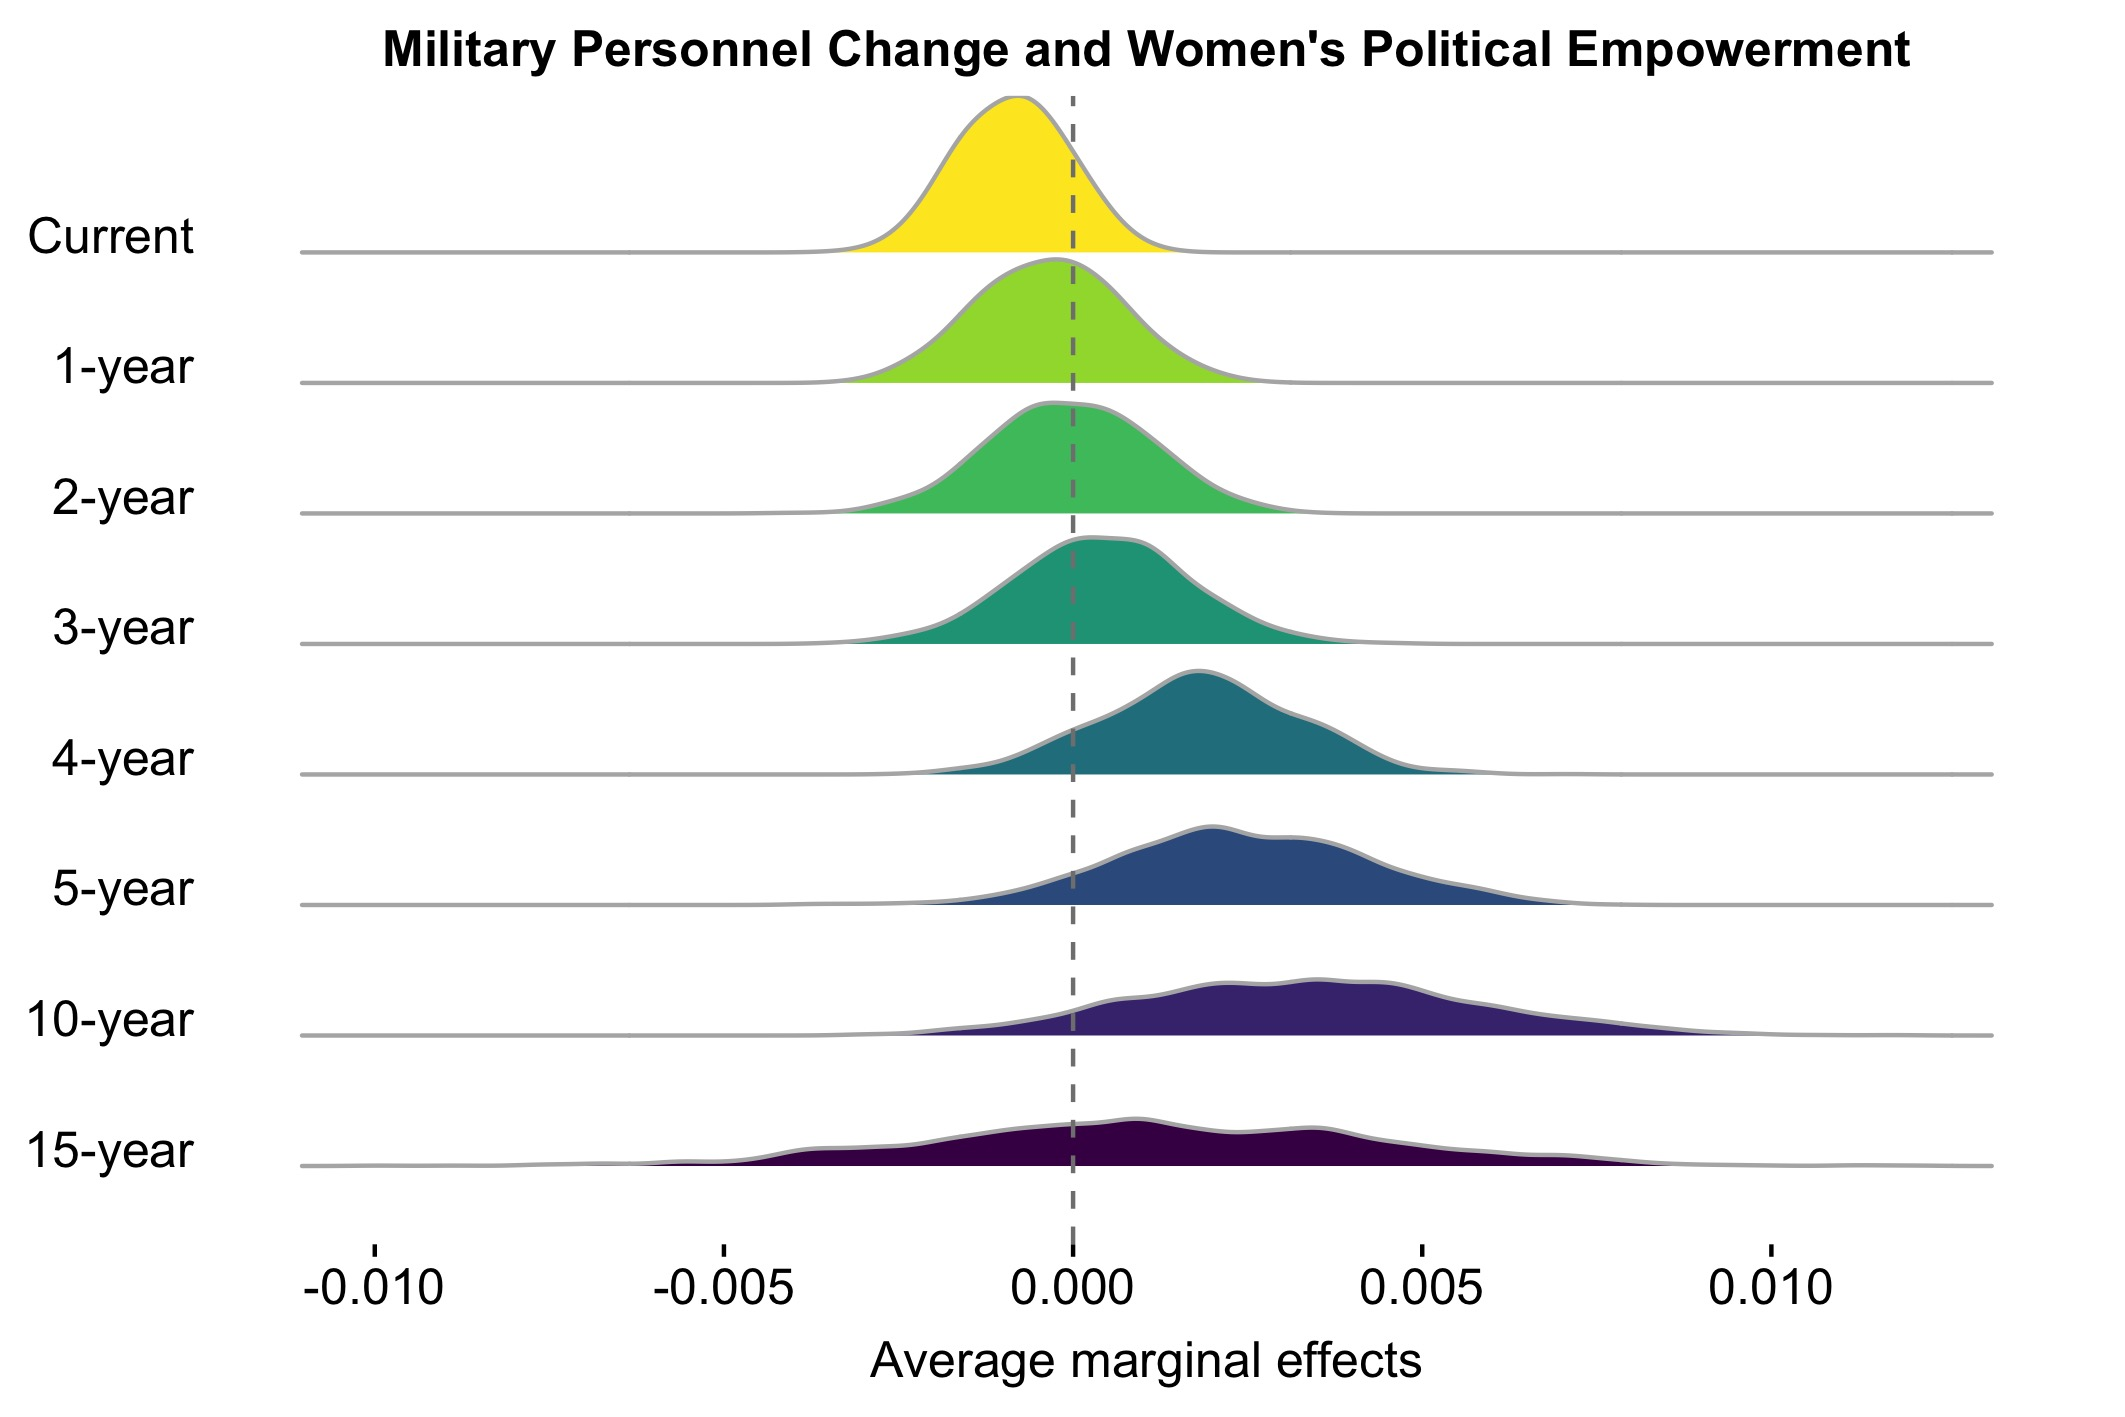
\includegraphics[scale=.1]{Fig7_s_lmilper_pc.jpg}}
   \subfigure[The marginal forward effects of population change on women's empowerment]{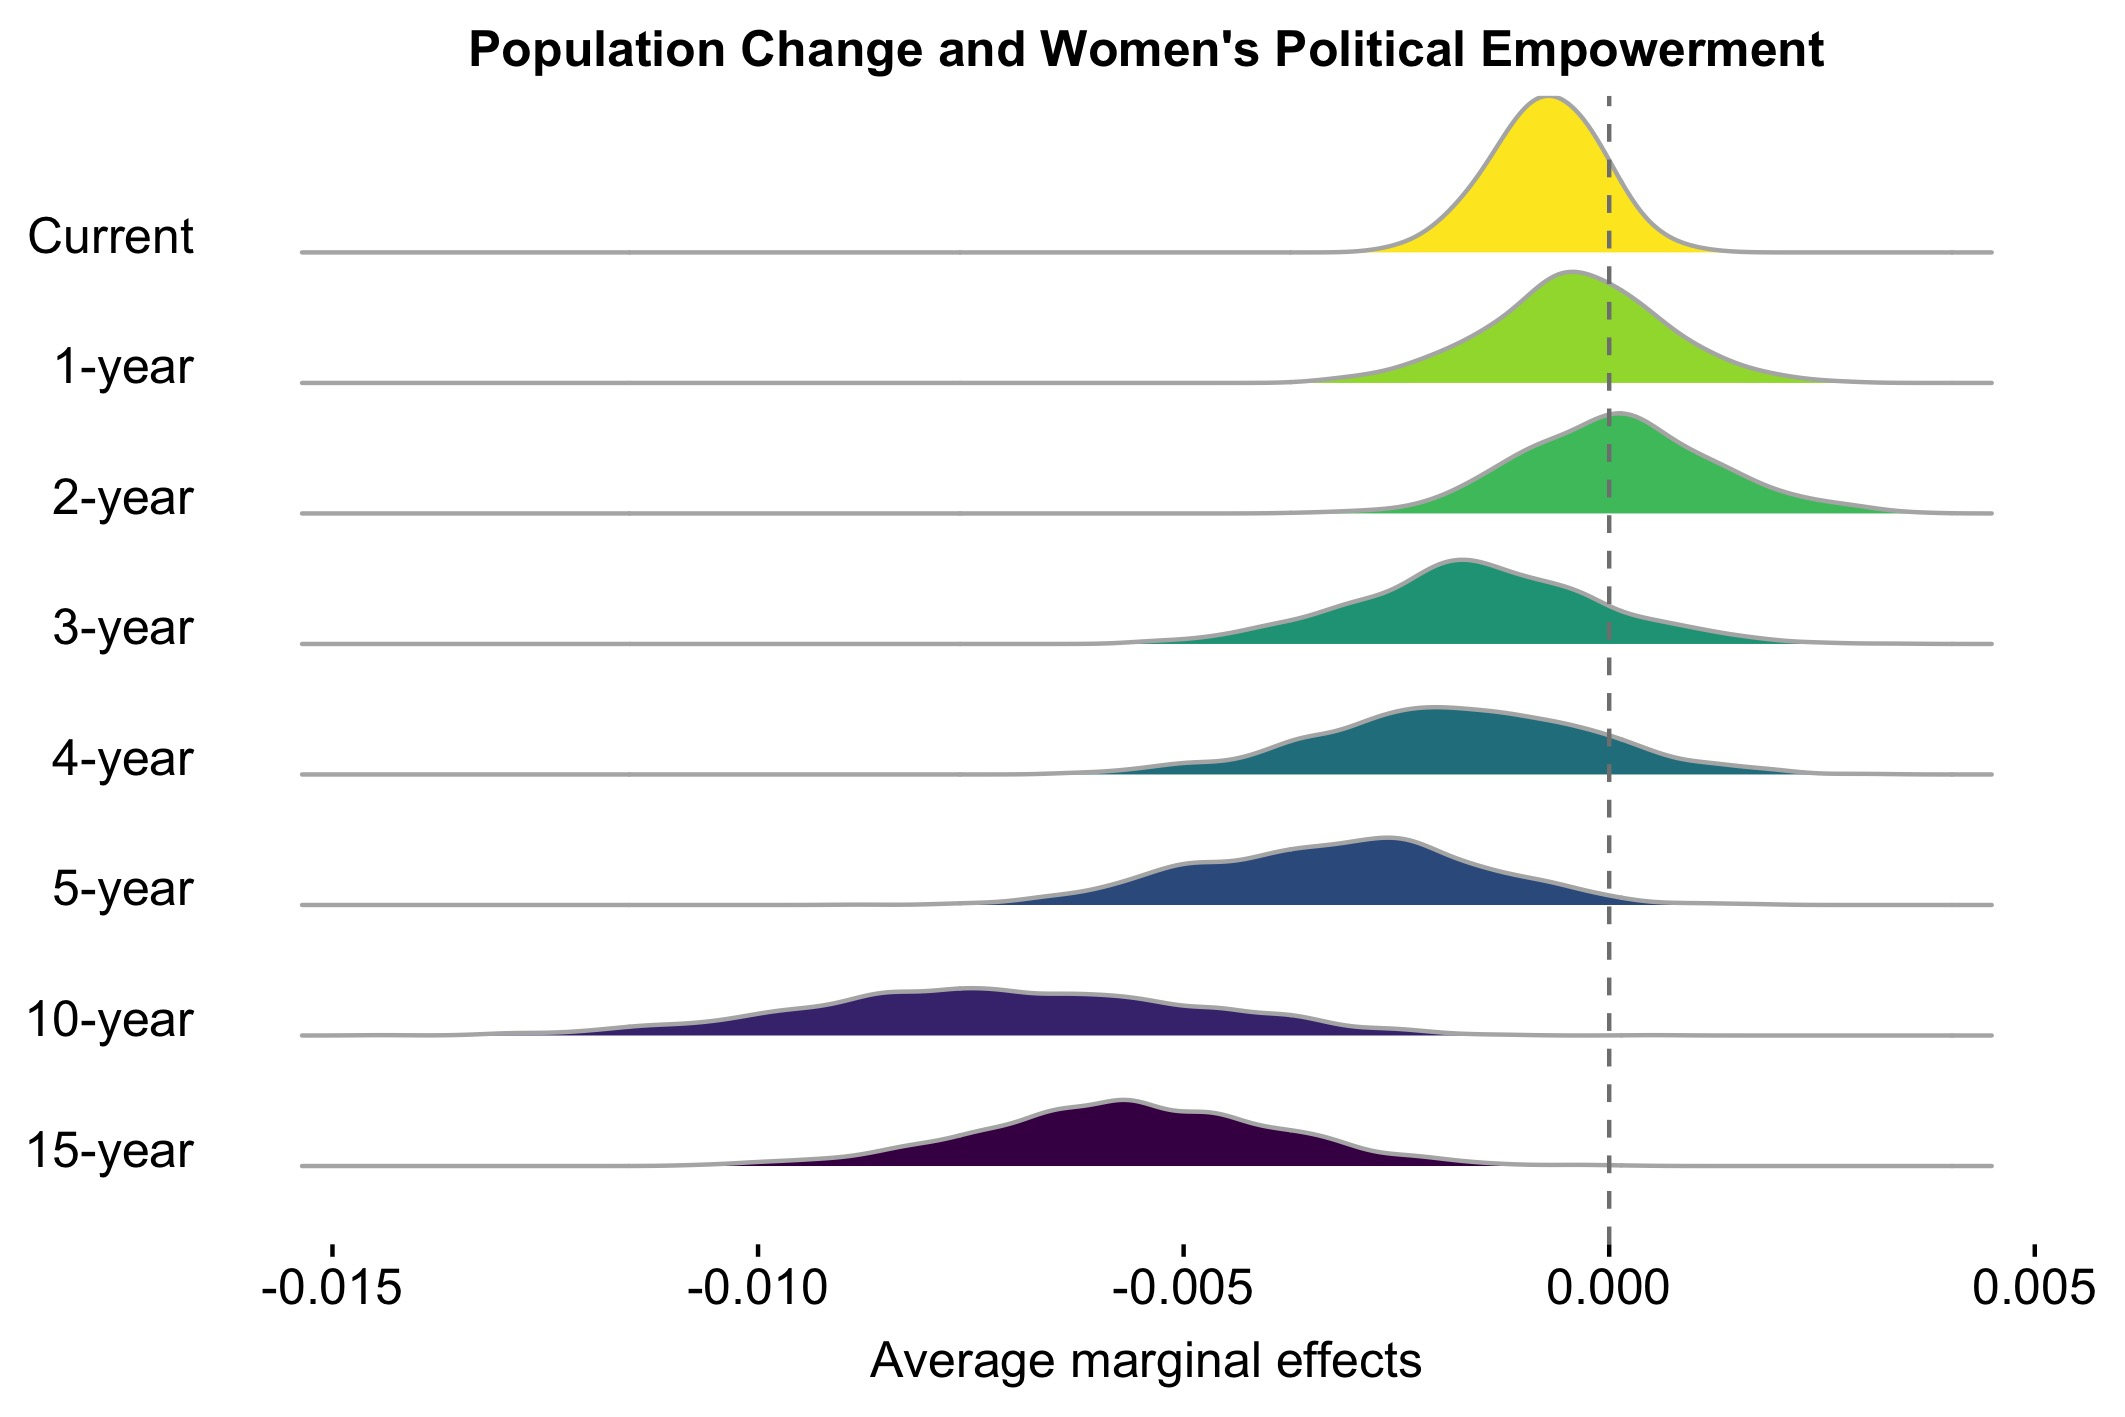
\includegraphics[scale=.1]{Fig7_s_lpop.jpg}}
   \subfigure[The marginal forward effects of irregular regime change on women's empowerment]{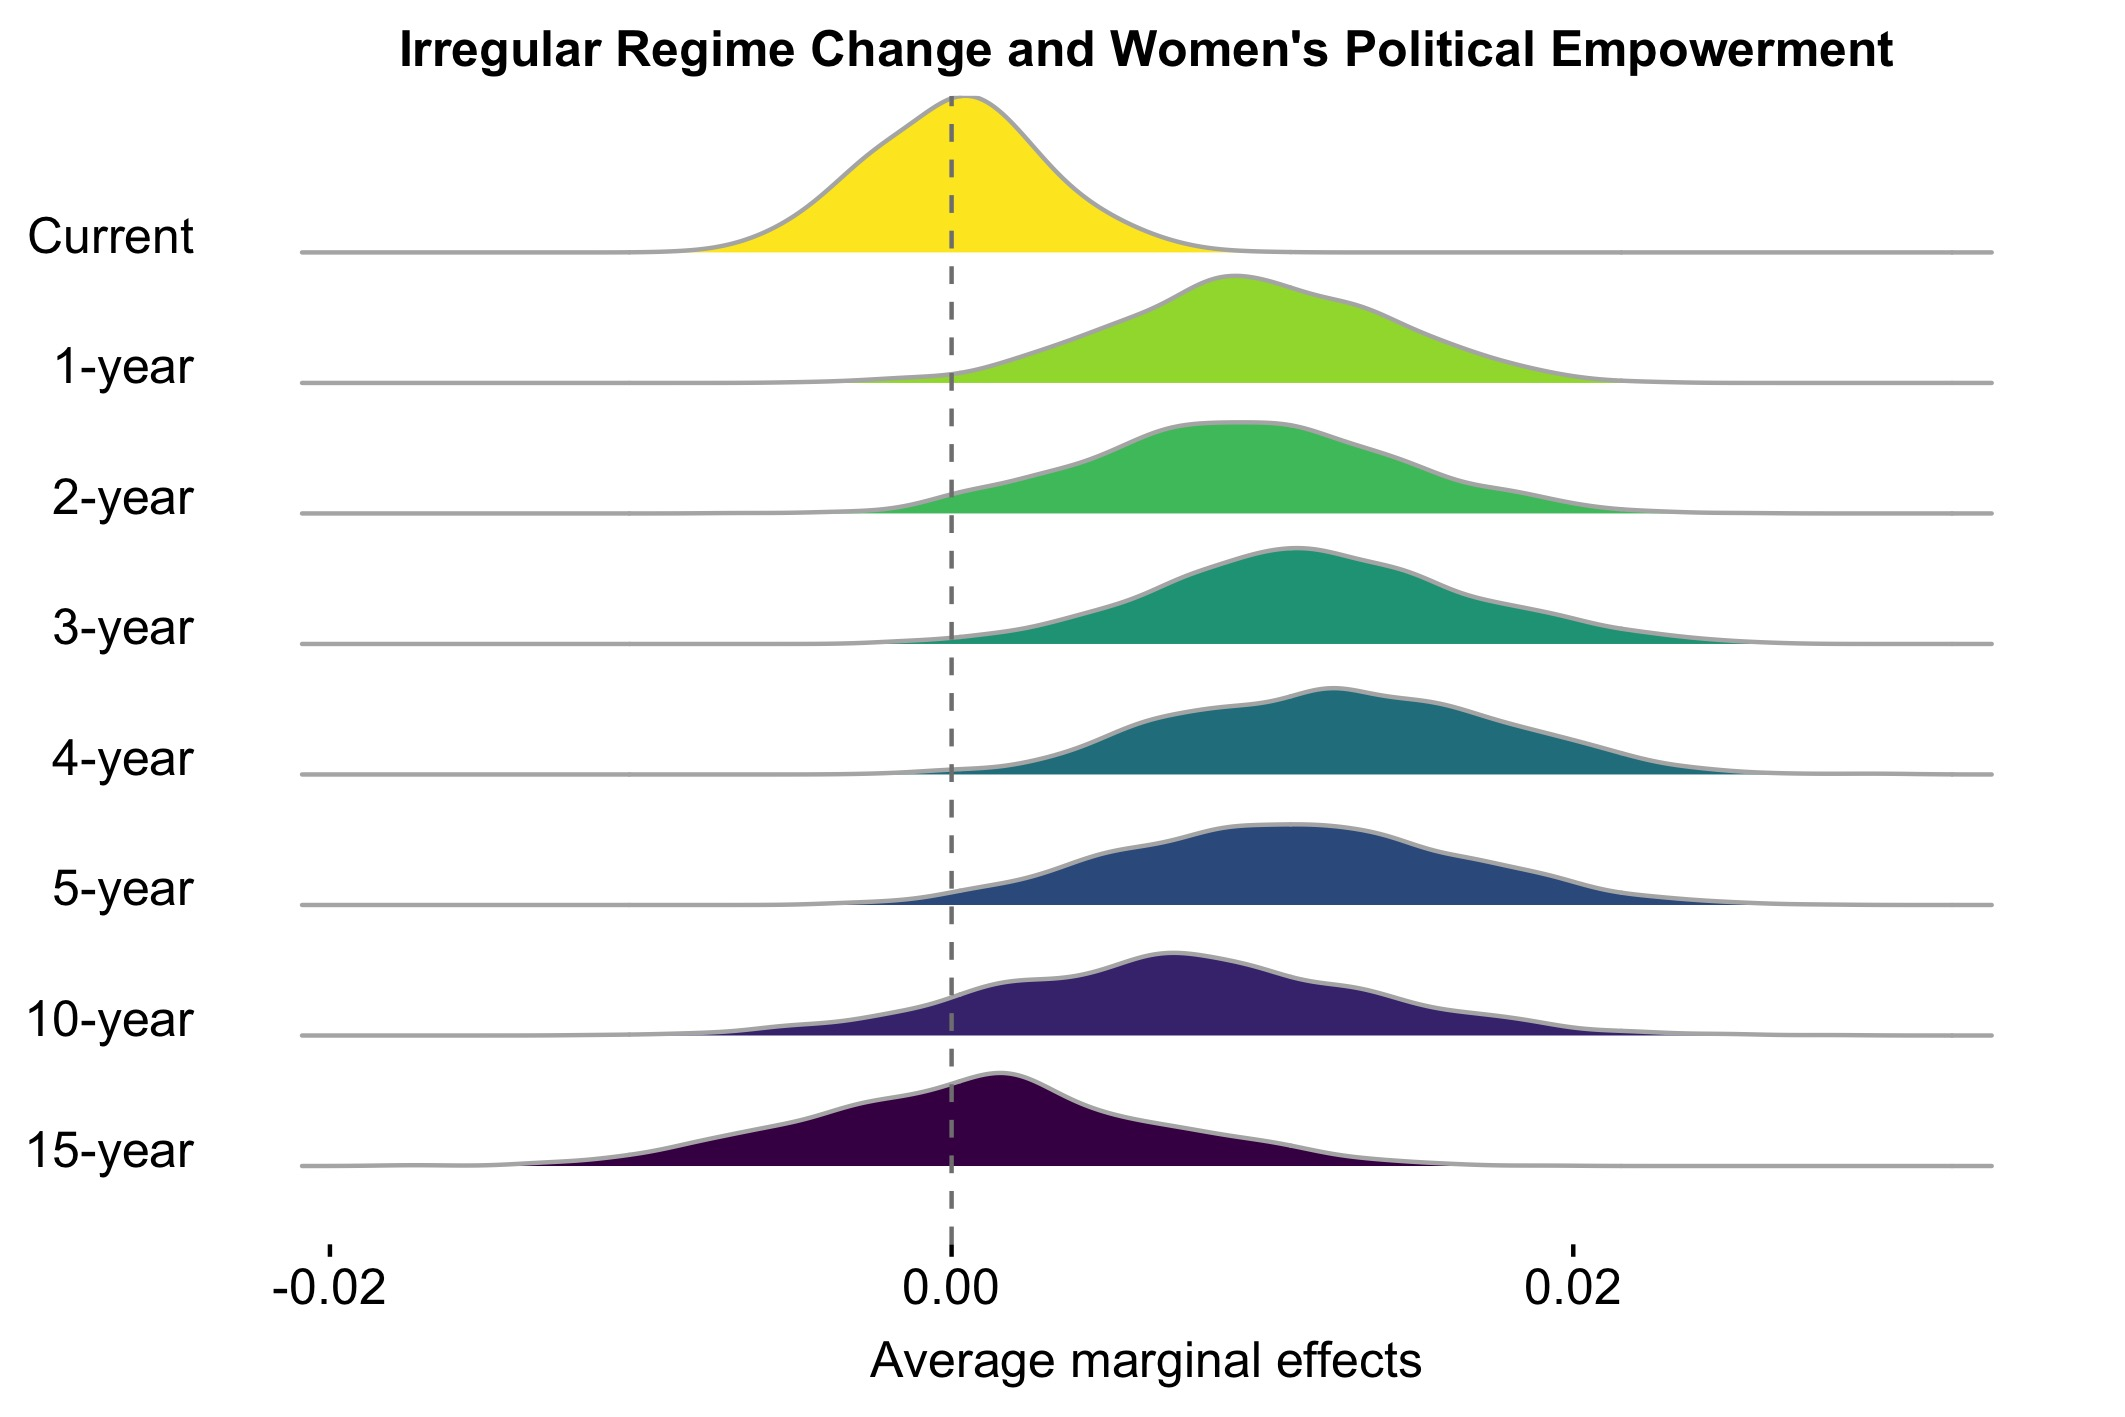
\includegraphics[scale=.1]{Fig7_irregular_dummy.jpg}}
   \subfigure[The marginal forward effects of war on women's empowerment]{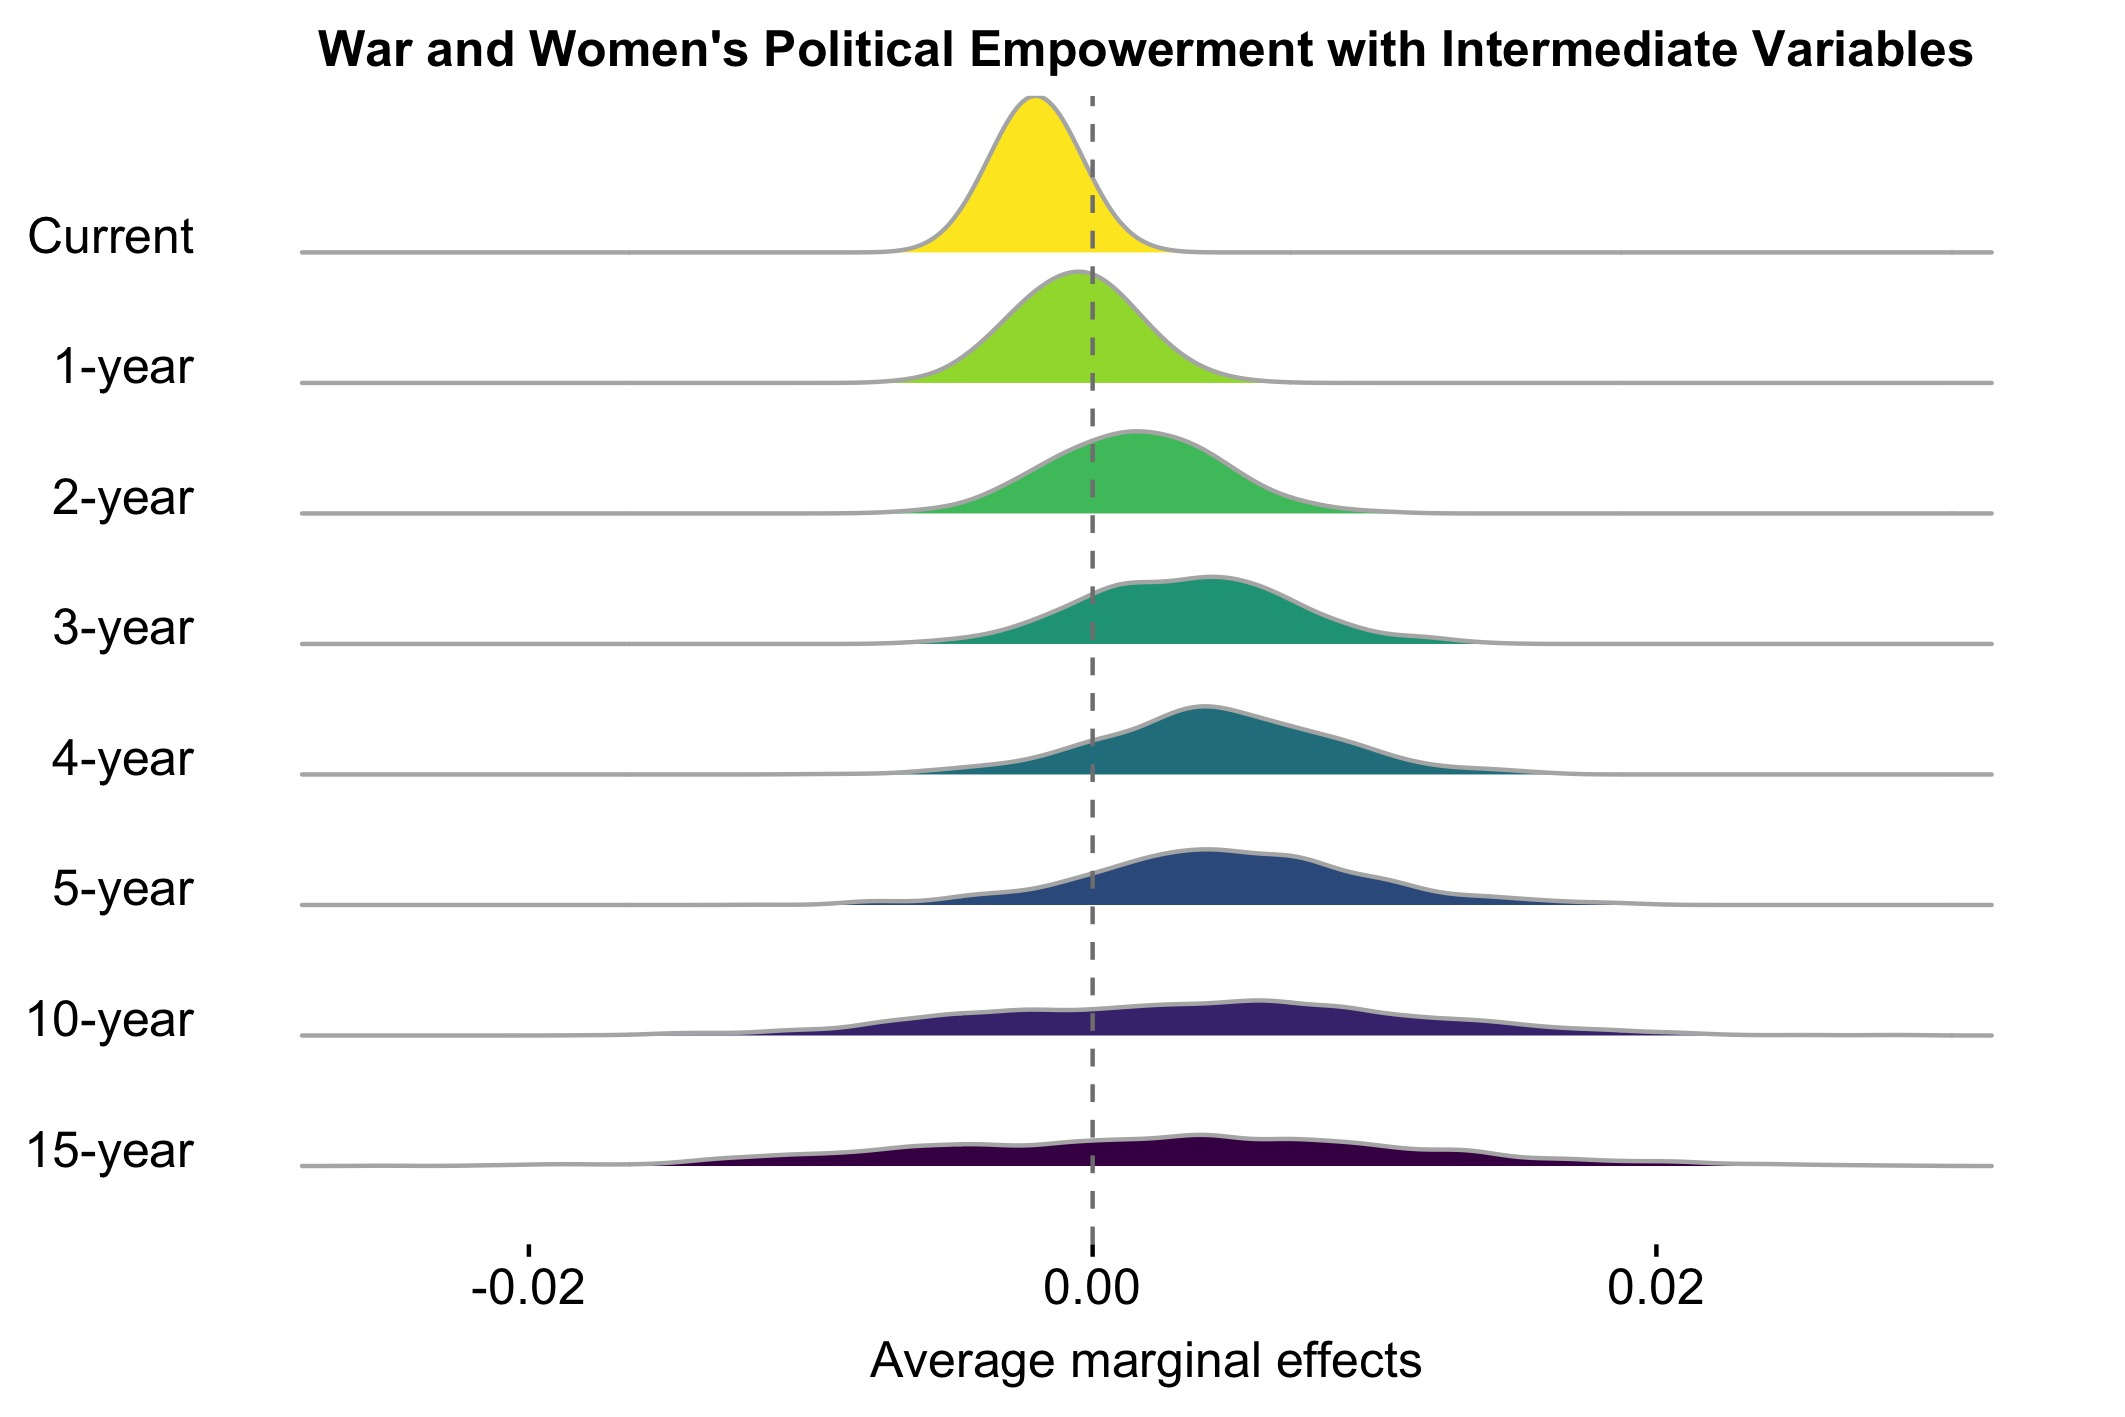
\includegraphics[scale=.1]{Fig7_warDummy.jpg}}
  \begin{flushleft}  
        {\footnotesize {\it Note}: Panel \emph{a} shows the effects of war on possible intermediate variables. The density plots are based on results in Table \ref{FEintermed}. Panels \emph{b} through \emph{d} shows the marginal forward effects of the possible intermediate variables when they are added to the core regression models in Table \ref{tab2}. Panel \emph{e} depicts the marginal forward effects of war once these intermediate variables are included in the model, based on results inTable \ref{intermpolempowerment}.}
       \end{flushleft} 
\end{figure}

\newpage
\appendix
%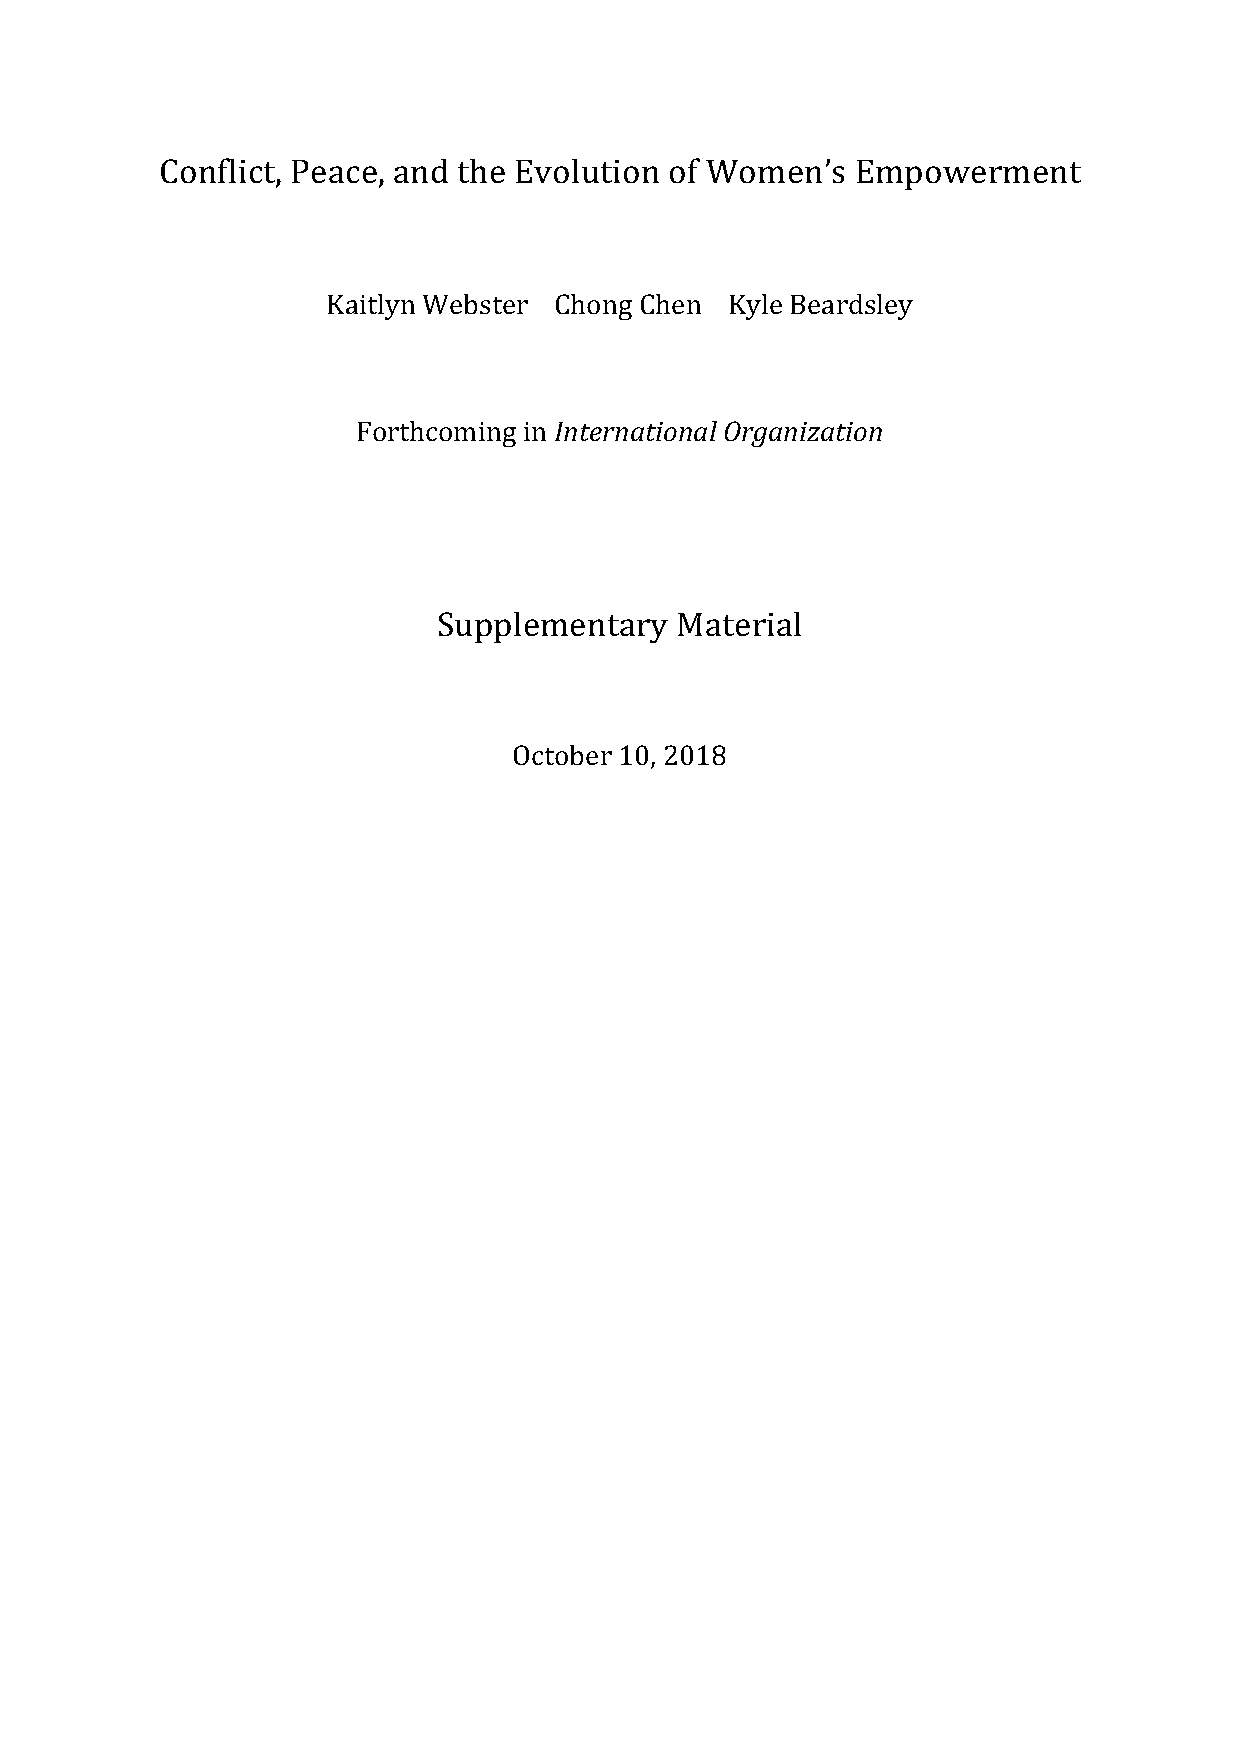
\includepdf[page={1}]{appendix_cover}[ht]
\tableofcontents
\addcontentsline{toc}{section}{Appendix}
\setcounter{page}{1}
\pagenumbering{Roman}
\section{Main Tables for Figures 3-7}
\appendixpagenumbering
\vspace*{.2in}
\setlength{\parskip}{-2em}
%\setlength{\parindent}{1cm}
\doublespacing
\setcounter{table}{0}
\setcounter{figure}{0}
\renewcommand{\thetable}{A\arabic{table}}	
\renewcommand{\thefigure}{A\arabic{figure}}	

Tables \ref{tab2}- \ref{intermpolempowerment} present coefficient estimates for all models across Figures 3-7 in our main text.  \\

% Fig 3(a) based on Models 1-8
%the main table for forward effect
{\renewcommand\normalsize{\tiny}% adjust table size
	\normalsize
\begin{table}[htbp]\centering
\def\sym#1{\ifmmode^{#1}\else\(^{#1}\)\fi}
\caption{Fixed-effects models of the effect of war on future changes in women's political empowerment\label{tab2}}
\begin{tabular}{l*{8}{c}}
\hline\hline
                    &\multicolumn{1}{c}{\shortstack{Model 1\\(current)}}&\multicolumn{1}{c}{\shortstack{Model 2\\(1-year)}}&\multicolumn{1}{c}{\shortstack{Model 3\\(2-year)}}&\multicolumn{1}{c}{\shortstack{Model 4\\(3-year)}}&\multicolumn{1}{c}{\shortstack{Model 5\\(4-year)}}&\multicolumn{1}{c}{\shortstack{Model 6\\(5-year)}}&\multicolumn{1}{c}{\shortstack{Model 7\\(10-year)}}&\multicolumn{1}{c}{\shortstack{Model 8\\(15-year)}}\\
\hline
War            &    -0.00155         &    0.000628         &     0.00346         &     0.00697\sym{*}  &     0.00930\sym{**} &      0.0101\sym{*}  &      0.0101         &     0.00506         \\
                    &   (0.00124)         &   (0.00209)         &   (0.00293)         &   (0.00360)         &   (0.00443)         &   (0.00523)         &   (0.00801)         &   (0.00916)         \\
[1em]
Political empowerment, lag   &     -0.0519\sym{***}&     -0.0949\sym{***}&      -0.140\sym{***}&      -0.189\sym{***}&      -0.236\sym{***}&      -0.286\sym{***}&      -0.508\sym{***}&      -0.675\sym{***}\\
                    &   (0.00484)         &   (0.00847)         &    (0.0118)         &    (0.0155)         &    (0.0189)         &    (0.0227)         &    (0.0381)         &    (0.0447)         \\
[1em]
$\Delta$Polity scores           &     0.00318\sym{***}&     0.00572\sym{***}&     0.00595\sym{***}&     0.00539\sym{***}&     0.00509\sym{***}&     0.00482\sym{***}&     0.00357\sym{***}&     0.00356\sym{***}\\
                    &  (0.000434)         &  (0.000759)         &  (0.000870)         &  (0.000869)         &  (0.000928)         &  (0.000895)         &  (0.000787)         &  (0.000835)         \\
[1em]
Polity scores, lag           &    0.000708\sym{***}&    0.000928\sym{***}&     0.00103\sym{***}&     0.00117\sym{***}&     0.00128\sym{***}&     0.00149\sym{***}&     0.00193\sym{**} &     0.00129         \\
                    & (0.0000937)         &  (0.000164)         &  (0.000231)         &  (0.000299)         &  (0.000362)         &  (0.000434)         &  (0.000783)         &  (0.000956)         \\
[1em]
$\Delta$Energy.consump,log           &    0.000444         &  -0.0000561         &   -0.000180         &   -0.000828         &    -0.00130         &    -0.00311         &    -0.00467         &    -0.00476         \\
                    &  (0.000834)         &  (0.000891)         &   (0.00109)         &   (0.00133)         &   (0.00158)         &   (0.00219)         &   (0.00309)         &   (0.00374)         \\
[1em]
Energy.consump, log, lag           &    0.000286         &    0.000555         &    0.000946         &     0.00138\sym{*}  &     0.00184\sym{*}  &     0.00231\sym{**} &     0.00478\sym{**} &     0.00799\sym{***}\\
                    &  (0.000205)         &  (0.000388)         &  (0.000586)         &  (0.000796)         &  (0.000984)         &   (0.00116)         &   (0.00204)         &   (0.00284)         \\
[1em]
Year               &    0.000253\sym{***}&    0.000507\sym{***}&    0.000777\sym{***}&     0.00107\sym{***}&     0.00134\sym{***}&     0.00162\sym{***}&     0.00290\sym{***}&     0.00384\sym{***}\\
                    & (0.0000295)         & (0.0000552)         & (0.0000819)         &  (0.000110)         &  (0.000135)         &  (0.000160)         &  (0.000283)         &  (0.000380)         \\
[1em]
$\Delta$Neighboring empowerment, lag&     0.00606\sym{*}  &      0.0189\sym{***}&      0.0227\sym{***}&      0.0238\sym{***}&      0.0190\sym{**} &      0.0224\sym{**} &      0.0144         &      0.0250\sym{*}  \\
                    &   (0.00361)         &   (0.00574)         &   (0.00853)         &   (0.00861)         &   (0.00834)         &   (0.00872)         &    (0.0139)         &    (0.0132)         \\
[1em]
Constant            &      -0.471\sym{***}&      -0.949\sym{***}&      -1.456\sym{***}&      -1.997\sym{***}&      -2.510\sym{***}&      -3.044\sym{***}&      -5.437\sym{***}&      -7.197\sym{***}\\
                    &    (0.0552)         &     (0.104)         &     (0.154)         &     (0.207)         &     (0.253)         &     (0.301)         &     (0.534)         &     (0.716)         \\
\hline
Observations        &        8090         &        7889         &        7708         &        7527         &        7362         &        7209         &        6538         &        6009         \\
\hline\hline
\multicolumn{9}{l}{\footnotesize Standard errors in parentheses}\\
\multicolumn{9}{l}{\footnotesize \sym{*} \(p<0.10\), \sym{**} \(p<0.05\), \sym{***} \(p<0.01\)}\\
\end{tabular}
\end{table}
 %label {tab2}  %index Models 1-8
}

% Fig 3(b-d) based on Models 9 -16
% the types of war
{\renewcommand\normalsize{\tiny}% adjust table size
	\normalsize
\begin{table}[htbp]\centering
\def\sym#1{\ifmmode^{#1}\else\(^{#1}\)\fi}
\caption{Fixed-effects models of the effect of war types on future changes in women's political empowerment\label{tab3}}
\begin{tabular}{l*{8}{c}}
\hline\hline
                    &\multicolumn{1}{c}{\shortstack{Model 9\\(current)}}&\multicolumn{1}{c}{\shortstack{Model 10\\(1-year)}}&\multicolumn{1}{c}{\shortstack{Model 11\\(2-year)}}&\multicolumn{1}{c}{\shortstack{Model 12\\(3-year)}}&\multicolumn{1}{c}{\shortstack{Model 13\\(4-year)}}&\multicolumn{1}{c}{\shortstack{Model 14\\(5-year)}}&\multicolumn{1}{c}{\shortstack{Model 15\\(10-year)}}&\multicolumn{1}{c}{\shortstack{Model 16\\(15-year)}}\\
\hline
New war              &    -0.00186         &   -0.000833         &    0.000581         &   -0.000171         &    0.000784         &     0.00338         &     0.00492         &     0.00203         \\
                    &   (0.00166)         &   (0.00277)         &   (0.00377)         &   (0.00460)         &   (0.00467)         &   (0.00490)         &   (0.00752)         &   (0.00887)         \\
[1em]
Ongoing war          &   -0.000645         &     0.00229         &     0.00588\sym{*}  &      0.0109\sym{**} &      0.0138\sym{**} &      0.0139\sym{**} &      0.0128         &     0.00639         \\
                    &   (0.00149)         &   (0.00244)         &   (0.00340)         &   (0.00443)         &   (0.00557)         &   (0.00662)         &   (0.00979)         &    (0.0110)         \\
[1em]
Recent war           &     0.00693\sym{***}&     0.00912\sym{***}&      0.0106\sym{**} &     0.00751\sym{*}  &     0.00752         &     0.00828         &     0.00389         &    0.000842         \\
                    &   (0.00228)         &   (0.00340)         &   (0.00411)         &   (0.00450)         &   (0.00481)         &   (0.00510)         &   (0.00723)         &   (0.00829)         \\
[1em]
Political empowerment, lag   &     -0.0514\sym{***}&     -0.0940\sym{***}&      -0.139\sym{***}&      -0.188\sym{***}&      -0.234\sym{***}&      -0.284\sym{***}&      -0.506\sym{***}&      -0.674\sym{***}\\
                    &   (0.00487)         &   (0.00842)         &    (0.0118)         &    (0.0154)         &    (0.0188)         &    (0.0225)         &    (0.0381)         &    (0.0450)         \\
[1em]
$\Delta$Polity scores            &     0.00319\sym{***}&     0.00572\sym{***}&     0.00596\sym{***}&     0.00538\sym{***}&     0.00508\sym{***}&     0.00482\sym{***}&     0.00356\sym{***}&     0.00356\sym{***}\\
                    &  (0.000433)         &  (0.000755)         &  (0.000867)         &  (0.000865)         &  (0.000926)         &  (0.000893)         &  (0.000787)         &  (0.000833)         \\
[1em]
Polity scores, lag              &    0.000700\sym{***}&    0.000915\sym{***}&     0.00102\sym{***}&     0.00115\sym{***}&     0.00126\sym{***}&     0.00147\sym{***}&     0.00191\sym{**} &     0.00128         \\
                    & (0.0000946)         &  (0.000164)         &  (0.000230)         &  (0.000298)         &  (0.000360)         &  (0.000432)         &  (0.000784)         &  (0.000958)         \\
[1em]
$\Delta$Energy.consump,log              &    0.000407         &   -0.000127         &   -0.000265         &    -0.00100         &    -0.00151         &    -0.00331         &    -0.00477         &    -0.00480         \\
                    &  (0.000835)         &  (0.000888)         &   (0.00108)         &   (0.00132)         &   (0.00158)         &   (0.00220)         &   (0.00310)         &   (0.00376)         \\
[1em]
Energy.consump, log, lag               &    0.000278         &    0.000548         &    0.000924         &     0.00135\sym{*}  &     0.00181\sym{*}  &     0.00227\sym{*}  &     0.00475\sym{**} &     0.00798\sym{***}\\
                    &  (0.000204)         &  (0.000390)         &  (0.000588)         &  (0.000796)         &  (0.000984)         &   (0.00116)         &   (0.00204)         &   (0.00284)         \\
[1em]
Year                &    0.000253\sym{***}&    0.000505\sym{***}&    0.000774\sym{***}&     0.00106\sym{***}&     0.00133\sym{***}&     0.00162\sym{***}&     0.00290\sym{***}&     0.00384\sym{***}\\
                    & (0.0000294)         & (0.0000551)         & (0.0000818)         &  (0.000109)         &  (0.000134)         &  (0.000160)         &  (0.000283)         &  (0.000380)         \\
[1em]
$\Delta$Neighboring empowerment, lag&     0.00611\sym{*}  &      0.0192\sym{***}&      0.0228\sym{***}&      0.0239\sym{***}&      0.0192\sym{**} &      0.0225\sym{**} &      0.0146         &      0.0250\sym{*}  \\
                    &   (0.00359)         &   (0.00575)         &   (0.00853)         &   (0.00864)         &   (0.00837)         &   (0.00872)         &    (0.0139)         &    (0.0132)         \\
[1em]
Constant            &      -0.470\sym{***}&      -0.946\sym{***}&      -1.451\sym{***}&      -1.987\sym{***}&      -2.499\sym{***}&      -3.035\sym{***}&      -5.431\sym{***}&      -7.194\sym{***}\\
                    &    (0.0550)         &     (0.103)         &     (0.154)         &     (0.206)         &     (0.253)         &     (0.301)         &     (0.535)         &     (0.717)         \\
\hline
Observations        &        8090         &        7889         &        7708         &        7527         &        7362         &        7209         &        6538         &        6009         \\
\hline\hline
\multicolumn{9}{l}{\footnotesize Standard errors in parentheses}\\
\multicolumn{9}{l}{\footnotesize \sym{*} \(p<0.10\), \sym{**} \(p<0.05\), \sym{***} \(p<0.01\)}\\
\end{tabular}
\end{table}
 %label {tab3}  % index models 9 -16
}


% Fig 4 based on Models 17-24
% IV model
\begin{landscape}
{\renewcommand\normalsize{\tiny}% adjust table size
	\normalsize
\begin{table}[htbp]\centering
\def\sym#1{\ifmmode^{#1}\else\(^{#1}\)\fi}
\caption{Endogenous treatment-regression models of the effect of war on future changes in women’s political empowerment\label{ivpolempowerment}}
\begin{tabular}{l*{8}{c}}
\hline\hline
                    &\multicolumn{1}{c}{\shortstack{Model 17\\(current)}}&\multicolumn{1}{c}{\shortstack{Model 18\\(1-year)}}&\multicolumn{1}{c}{\shortstack{Model 19\\(2-year)}}&\multicolumn{1}{c}{\shortstack{Model 20\\(3-year)}}&\multicolumn{1}{c}{\shortstack{Model 21\\(4-year)}}&\multicolumn{1}{c}{\shortstack{Model 22\\(5-year)}}&\multicolumn{1}{c}{\shortstack{Model 23\\(10-year)}}&\multicolumn{1}{c}{\shortstack{Model 24\\(15-year)}}\\
\hline
$\Delta$Polity scores        &     0.00311\sym{***}&     0.00556\sym{***}&     0.00586\sym{***}&     0.00535\sym{***}&     0.00521\sym{***}&     0.00501\sym{***}&     0.00322\sym{***}&     0.00345\sym{***}\\
                    &  (0.000434)         &  (0.000753)         &  (0.000883)         &  (0.000917)         &   (0.00103)         &   (0.00102)         &  (0.000854)         &  (0.000855)         \\
[1em]
Polity scores, lag           &    0.000135\sym{***}&   0.0000566         &  -0.0000718         &   -0.000197         &   -0.000333\sym{*}  &   -0.000453\sym{**} &    -0.00124\sym{***}&    -0.00209\sym{***}\\
                    & (0.0000465)         & (0.0000744)         &  (0.000108)         &  (0.000143)         &  (0.000179)         &  (0.000216)         &  (0.000425)         &  (0.000635)         \\
[1em]
$\Delta$Energy.consump,log             &    0.000828         &    0.000435         &    0.000310         &   -0.000400         &    -0.00102         &    -0.00250         &    -0.00579\sym{**} &    -0.00518         \\
                    &  (0.000923)         &   (0.00107)         &   (0.00126)         &   (0.00138)         &   (0.00164)         &   (0.00217)         &   (0.00268)         &   (0.00319)         \\
[1em]
Energy.consump,log, lag             &   -0.000209\sym{**} &  -0.0000758         &   0.0000934         &    0.000229         &    0.000344         &    0.000472         &     0.00232\sym{***}&     0.00445\sym{***}\\
                    &  (0.000105)         &  (0.000177)         &  (0.000261)         &  (0.000327)         &  (0.000384)         &  (0.000447)         &  (0.000804)         &   (0.00124)         \\
[1em]
Year                &   0.0000579\sym{***}&    0.000108\sym{***}&    0.000163\sym{***}&    0.000223\sym{***}&    0.000287\sym{***}&    0.000359\sym{***}&    0.000606\sym{***}&    0.000830\sym{***}\\
                    & (0.0000113)         & (0.0000195)         & (0.0000284)         & (0.0000366)         & (0.0000443)         & (0.0000546)         & (0.0000912)         &  (0.000144)         \\
[1em]
War         &      0.0272\sym{***}&      0.0346\sym{***}&      0.0417\sym{**} &      0.0526\sym{**} &      0.0651\sym{***}&      0.0735\sym{***}&      0.0282         &      0.0144         \\
                    &   (0.00384)         &    (0.0108)         &    (0.0190)         &    (0.0223)         &    (0.0217)         &    (0.0248)         &    (0.0172)         &    (0.0136)         \\
[1em]
Constant            &      -0.111\sym{***}&      -0.206\sym{***}&      -0.312\sym{***}&      -0.428\sym{***}&      -0.549\sym{***}&      -0.688\sym{***}&      -1.154\sym{***}&      -1.576\sym{***}\\
                    &    (0.0220)         &    (0.0382)         &    (0.0559)         &    (0.0718)         &    (0.0868)         &     (0.107)         &     (0.178)         &     (0.281)         \\
\hline
Treatment = War                &                     &                     &                     &                     &                     &                     &                     &                     \\
Neigh.civil.war, count, lag&       0.114\sym{***}&      0.0869\sym{*}  &      0.0635         &      0.0760         &      0.0653         &      0.0727         &     0.00943         &      0.0553         \\
                    &    (0.0432)         &    (0.0521)         &    (0.0542)         &    (0.0561)         &    (0.0536)         &    (0.0534)         &    (0.0639)         &    (0.0664)         \\
[1em]
Neigh.civil.war, count, 2 lags&      0.0580         &      0.0869         &       0.104\sym{*}  &      0.0968\sym{*}  &      0.0925\sym{*}  &      0.0745         &       0.136\sym{*}  &       0.109         \\
                    &    (0.0445)         &    (0.0531)         &    (0.0553)         &    (0.0571)         &    (0.0563)         &    (0.0585)         &    (0.0738)         &    (0.0736)         \\
[1em]
Neigh.interstate.wars, count, lag&       0.309\sym{***}&       0.319\sym{***}&       0.369\sym{***}&       0.373\sym{***}&       0.371\sym{***}&       0.391\sym{***}&       0.408\sym{***}&       0.435\sym{***}\\
                    &    (0.0657)         &    (0.0965)         &    (0.0939)         &    (0.0920)         &    (0.0890)         &    (0.0885)         &    (0.0725)         &    (0.0804)         \\
[1em]
Neigh.interstate.wars, count, 2 lags&      0.0268         &      0.0655         &      0.0564         &      0.0604         &      0.0612         &      0.0345         &      0.0149         &     -0.0631         \\
                    &    (0.0499)         &    (0.0588)         &    (0.0490)         &    (0.0496)         &    (0.0505)         &    (0.0446)         &    (0.0557)         &    (0.0619)         \\
[1em]
$\Delta$Polity scores            &     -0.0387\sym{**} &     -0.0446\sym{**} &     -0.0403         &     -0.0431\sym{**} &     -0.0509\sym{***}&     -0.0461\sym{**} &     -0.0364\sym{***}&     -0.0236\sym{*}  \\
                    &    (0.0169)         &    (0.0227)         &    (0.0255)         &    (0.0207)         &    (0.0195)         &    (0.0186)         &    (0.0140)         &    (0.0139)         \\
[1em]
Polity scores, lag             &    -0.00943         &    -0.00918         &    -0.00904         &    -0.00864         &    -0.00793         &    -0.00754         &    -0.00991         &    -0.00917         \\
                    &   (0.00613)         &   (0.00659)         &   (0.00693)         &   (0.00719)         &   (0.00730)         &   (0.00749)         &   (0.00766)         &   (0.00769)         \\
[1em]
$\Delta$Energy.consump,log             &     -0.0464         &     -0.0636         &     -0.0779         &     -0.0833         &     -0.0867         &      -0.115         &      -0.120         &      -0.129         \\
                    &    (0.0654)         &    (0.0663)         &    (0.0725)         &    (0.0918)         &    (0.0915)         &     (0.110)         &     (0.107)         &     (0.106)         \\
[1em]
Energy.consump,log, lag              &      0.0526\sym{***}&      0.0524\sym{***}&      0.0538\sym{***}&      0.0527\sym{***}&      0.0515\sym{***}&      0.0527\sym{***}&      0.0753\sym{***}&      0.0657\sym{***}\\
                    &    (0.0139)         &    (0.0152)         &    (0.0164)         &    (0.0168)         &    (0.0171)         &    (0.0174)         &    (0.0163)         &    (0.0150)         \\
[1em]
Year                &    -0.00376\sym{***}&    -0.00327\sym{**} &    -0.00305\sym{*}  &    -0.00290\sym{*}  &    -0.00257         &    -0.00291\sym{*}  &    -0.00243         &    -0.00207         \\
                    &   (0.00139)         &   (0.00157)         &   (0.00163)         &   (0.00162)         &   (0.00164)         &   (0.00168)         &   (0.00198)         &   (0.00210)         \\
[1em]
Constant            &       5.702\sym{**} &       4.677         &       4.212         &       3.914         &       3.300         &       3.969         &       2.800         &       2.175         \\
                    &     (2.709)         &     (3.061)         &     (3.198)         &     (3.170)         &     (3.199)         &     (3.268)         &     (3.844)         &     (4.065)         \\
\hline
ath$\rho$               &      -0.758\sym{***}&      -0.572\sym{**} &      -0.505\sym{*}  &      -0.512\sym{*}  &      -0.559\sym{**} &      -0.567\sym{**} &     -0.0713         &    -0.00461         \\
                    &     (0.126)         &     (0.223)         &     (0.302)         &     (0.303)         &     (0.267)         &     (0.280)         &     (0.104)         &    (0.0524)         \\
[1em]
lnsigma             &      -3.750\sym{***}&      -3.393\sym{***}&      -3.174\sym{***}&      -3.013\sym{***}&      -2.885\sym{***}&      -2.785\sym{***}&      -2.506\sym{***}&      -2.329\sym{***}\\
                    &    (0.0575)         &    (0.0681)         &    (0.0759)         &    (0.0786)         &    (0.0782)         &    (0.0816)         &    (0.0620)         &    (0.0633)         \\
\hline
Observations        &        8090         &        7889         &        7708         &        7527         &        7362         &        7209         &        6538         &        6009         \\
\hline\hline
\multicolumn{9}{l}{\footnotesize Standard errors in parentheses}\\
\multicolumn{9}{l}{\footnotesize \sym{*} \(p<0.10\), \sym{**} \(p<0.05\), \sym{***} \(p<0.01\)}\\
\end{tabular}
\end{table}
 %label {ivpolempowerment} % index models 17-24
}
\end{landscape}

% Fig 5(a) based Models 25-32
% war duration and women's empowerment
{\renewcommand\normalsize{\tiny}% adjust table size
	\normalsize
\begin{table}[htbp]\centering
\def\sym#1{\ifmmode^{#1}\else\(^{#1}\)\fi}
\caption{Fixed-effects models of the effect of war duration on future changes in women's political empowerment\label{polwardur}}
\begin{tabular}{l*{8}{c}}
\hline\hline
                    &\multicolumn{1}{c}{\shortstack{Model 25\\(current)}}&\multicolumn{1}{c}{\shortstack{Model 26\\(1-year)}}&\multicolumn{1}{c}{\shortstack{Model 27\\(2-year)}}&\multicolumn{1}{c}{\shortstack{Model 28\\(3-year)}}&\multicolumn{1}{c}{\shortstack{Model 29\\(4-year)}}&\multicolumn{1}{c}{\shortstack{Model 30\\(5-year)}}&\multicolumn{1}{c}{\shortstack{Model 31\\(10-year)}}&\multicolumn{1}{c}{\shortstack{Model 32\\(15-year)}}\\
\hline
War duration             &    0.000258\sym{*}  &    0.000782\sym{***}&     0.00127\sym{***}&     0.00173\sym{***}&     0.00198\sym{***}&     0.00205\sym{***}&     0.00172         &     0.00139         \\
                    &  (0.000152)         &  (0.000235)         &  (0.000347)         &  (0.000508)         &  (0.000649)         &  (0.000751)         &   (0.00116)         &   (0.00121)         \\
[1em]
Political empowerment, lag  &     -0.0509\sym{***}&     -0.0940\sym{***}&      -0.139\sym{***}&      -0.189\sym{***}&      -0.236\sym{***}&      -0.286\sym{***}&      -0.506\sym{***}&      -0.673\sym{***}\\
                    &   (0.00481)         &   (0.00841)         &    (0.0118)         &    (0.0155)         &    (0.0189)         &    (0.0226)         &    (0.0381)         &    (0.0440)         \\
[1em]
$\Delta$Polity scores            &     0.00319\sym{***}&     0.00574\sym{***}&     0.00598\sym{***}&     0.00540\sym{***}&     0.00509\sym{***}&     0.00484\sym{***}&     0.00355\sym{***}&     0.00354\sym{***}\\
                    &  (0.000435)         &  (0.000760)         &  (0.000871)         &  (0.000870)         &  (0.000929)         &  (0.000897)         &  (0.000793)         &  (0.000838)         \\
[1em]
Polity scores, lag           &    0.000700\sym{***}&    0.000924\sym{***}&     0.00104\sym{***}&     0.00119\sym{***}&     0.00130\sym{***}&     0.00151\sym{***}&     0.00190\sym{**} &     0.00125         \\
                    & (0.0000939)         &  (0.000163)         &  (0.000228)         &  (0.000295)         &  (0.000356)         &  (0.000428)         &  (0.000781)         &  (0.000948)         \\
[1em]
$\Delta$Energy.consump,log           &    0.000443         &   -0.000129         &   -0.000315         &    -0.00110         &    -0.00168         &    -0.00352         &    -0.00494         &    -0.00489         \\
                    &  (0.000849)         &  (0.000922)         &   (0.00110)         &   (0.00134)         &   (0.00158)         &   (0.00218)         &   (0.00310)         &   (0.00378)         \\
[1em]
Energy.consump,log, lag             &    0.000255         &    0.000511         &    0.000887         &     0.00131\sym{*}  &     0.00177\sym{*}  &     0.00223\sym{*}  &     0.00477\sym{**} &     0.00796\sym{***}\\
                    &  (0.000207)         &  (0.000386)         &  (0.000581)         &  (0.000787)         &  (0.000973)         &   (0.00115)         &   (0.00204)         &   (0.00285)         \\
[1em]
Year                &    0.000251\sym{***}&    0.000504\sym{***}&    0.000772\sym{***}&     0.00106\sym{***}&     0.00133\sym{***}&     0.00162\sym{***}&     0.00289\sym{***}&     0.00382\sym{***}\\
                    & (0.0000293)         & (0.0000550)         & (0.0000819)         &  (0.000110)         &  (0.000135)         &  (0.000160)         &  (0.000284)         &  (0.000378)         \\
[1em]
$\Delta$Neighboring empowerment, lag&     0.00573         &      0.0185\sym{***}&      0.0227\sym{***}&      0.0237\sym{***}&      0.0195\sym{**} &      0.0230\sym{***}&      0.0154         &      0.0256\sym{*}  \\
                    &   (0.00360)         &   (0.00574)         &   (0.00861)         &   (0.00870)         &   (0.00845)         &   (0.00877)         &    (0.0140)         &    (0.0132)         \\
[1em]
Constant            &      -0.467\sym{***}&      -0.942\sym{***}&      -1.446\sym{***}&      -1.985\sym{***}&      -2.498\sym{***}&      -3.030\sym{***}&      -5.411\sym{***}&      -7.168\sym{***}\\
                    &    (0.0550)         &     (0.103)         &     (0.154)         &     (0.207)         &     (0.254)         &     (0.302)         &     (0.535)         &     (0.714)         \\
\hline
Observations        &        8062         &        7861         &        7680         &        7498         &        7333         &        7180         &        6509         &        5980         \\
\hline\hline
\multicolumn{9}{l}{\footnotesize Standard errors in parentheses}\\
\multicolumn{9}{l}{\footnotesize \sym{*} \(p<0.10\), \sym{**} \(p<0.05\), \sym{***} \(p<0.01\)}\\
\end{tabular}
\end{table}
 %label {polwardur} % index models  25-32
}

%Fig 5(b) based on Models 33-40
% battle deaths
{\renewcommand\normalsize{\tiny}% adjust table size
	\normalsize
\begin{table}[htbp]\centering
\def\sym#1{\ifmmode^{#1}\else\(^{#1}\)\fi}
\caption{Fixed-effects models of the effect of battle deaths on future changes in women's political empowerment\label{polbdeath}}
\begin{tabular}{l*{8}{c}}
\hline\hline
                    &\multicolumn{1}{c}{\shortstack{Model 33\\(current)}}&\multicolumn{1}{c}{\shortstack{Model 34\\(1-year)}}&\multicolumn{1}{c}{\shortstack{Model 35\\(2-year)}}&\multicolumn{1}{c}{\shortstack{Model 36\\(3-year)}}&\multicolumn{1}{c}{\shortstack{Model 37\\(4-year)}}&\multicolumn{1}{c}{\shortstack{Model 38\\(5-year)}}&\multicolumn{1}{c}{\shortstack{Model 39\\(10-year)}}&\multicolumn{1}{c}{\shortstack{Model 40\\(15-year)}}\\
\hline
Battle deaths, log        &   -0.000532\sym{*}  &   -0.000508         &   -0.000514         &   -0.000356         &  -0.0000202         &   -0.000159         &    0.000192         &     0.00156         \\
                    &  (0.000275)         &  (0.000444)         &  (0.000583)         &  (0.000747)         &  (0.000935)         &   (0.00113)         &   (0.00125)         &   (0.00145)         \\
[1em]
Political empowerment, lag  &     -0.0739\sym{***}&      -0.134\sym{***}&      -0.192\sym{***}&      -0.249\sym{***}&      -0.301\sym{***}&      -0.360\sym{***}&      -0.617\sym{***}&      -0.810\sym{***}\\
                    &   (0.00693)         &    (0.0112)         &    (0.0157)         &    (0.0198)         &    (0.0233)         &    (0.0272)         &    (0.0414)         &    (0.0450)         \\
[1em]
$\Delta$Polity scores          &     0.00370\sym{***}&     0.00641\sym{***}&     0.00649\sym{***}&     0.00590\sym{***}&     0.00541\sym{***}&     0.00483\sym{***}&     0.00373\sym{***}&     0.00355\sym{***}\\
                    &  (0.000595)         &  (0.000937)         &   (0.00104)         &  (0.000984)         &  (0.000968)         &  (0.000922)         &  (0.000774)         &  (0.000685)         \\
[1em]
Polity scores, lag          &     0.00109\sym{***}&     0.00151\sym{***}&     0.00173\sym{***}&     0.00191\sym{***}&     0.00204\sym{***}&     0.00228\sym{***}&     0.00331\sym{***}&     0.00293\sym{***}\\
                    &  (0.000135)         &  (0.000222)         &  (0.000296)         &  (0.000362)         &  (0.000419)         &  (0.000486)         &  (0.000830)         &  (0.000949)         \\
[1em]
$\Delta$Energy.consump,log             &    0.000109         &   -0.000193         &   -0.000539         &   -0.000828         &   -0.000851         &    -0.00116         &    -0.00171         &    -0.00269         \\
                    &  (0.000746)         &  (0.000895)         &   (0.00122)         &   (0.00147)         &   (0.00171)         &   (0.00244)         &   (0.00295)         &   (0.00368)         \\
[1em]
Energy.consump,log, lag             &    0.000280         &    0.000415         &    0.000749         &     0.00131         &     0.00206         &     0.00293\sym{*}  &     0.00530\sym{**} &     0.00737\sym{**} \\
                    &  (0.000295)         &  (0.000536)         &  (0.000806)         &   (0.00108)         &   (0.00132)         &   (0.00157)         &   (0.00266)         &   (0.00356)         \\
[1em]
Year                &    0.000358\sym{***}&    0.000735\sym{***}&     0.00111\sym{***}&     0.00146\sym{***}&     0.00177\sym{***}&     0.00211\sym{***}&     0.00377\sym{***}&     0.00515\sym{***}\\
                    & (0.0000502)         & (0.0000905)         &  (0.000137)         &  (0.000181)         &  (0.000224)         &  (0.000272)         &  (0.000478)         &  (0.000689)         \\
[1em]
$\Delta$Neighboring  empowerment, lag &     0.00892\sym{**} &      0.0204\sym{***}&      0.0249\sym{***}&      0.0264\sym{***}&      0.0212\sym{**} &      0.0290\sym{***}&      0.0239\sym{*}  &      0.0363\sym{**} \\
                    &   (0.00424)         &   (0.00658)         &   (0.00951)         &   (0.00994)         &   (0.01000)         &    (0.0107)         &    (0.0137)         &    (0.0141)         \\
[1em]
Constant            &      -0.666\sym{***}&      -1.378\sym{***}&      -2.083\sym{***}&      -2.744\sym{***}&      -3.333\sym{***}&      -3.967\sym{***}&      -7.115\sym{***}&      -9.730\sym{***}\\
                    &    (0.0954)         &     (0.172)         &     (0.262)         &     (0.347)         &     (0.428)         &     (0.521)         &     (0.918)         &     (1.326)         \\
\hline
Observations        &        5938         &        5853         &        5798         &        5752         &        5728         &        5651         &        5101         &        4569         \\
\hline\hline
\multicolumn{9}{l}{\footnotesize Standard errors in parentheses}\\
\multicolumn{9}{l}{\footnotesize \sym{*} \(p<0.10\), \sym{**} \(p<0.05\), \sym{***} \(p<0.01\)}\\
\end{tabular}
\end{table}
 %label {polbdeath} % index models  33-40
}

% Fig 6(a) based on Models 41-48
% fertility rates
{\renewcommand\normalsize{\tiny}% adjust table size
	\normalsize
\begin{table}[htbp]\centering
\def\sym#1{\ifmmode^{#1}\else\(^{#1}\)\fi}
\caption{Fixed-effects models of the effect of war on future changes in fertility rates\label{fefertility}}
\begin{tabular}{l*{8}{c}}
\hline\hline
                    &\multicolumn{1}{c}{\shortstack{Model 41\\(current)}}&\multicolumn{1}{c}{\shortstack{Model 42\\(1-year)}}&\multicolumn{1}{c}{\shortstack{Model 43\\(2-year)}}&\multicolumn{1}{c}{\shortstack{Model 44\\(3-year)}}&\multicolumn{1}{c}{\shortstack{Model 45\\(4-year)}}&\multicolumn{1}{c}{\shortstack{Model 46\\(5-year)}}&\multicolumn{1}{c}{\shortstack{Model 47\\(10-year)}}&\multicolumn{1}{c}{\shortstack{Model 48\\(15-year)}}\\
\hline
War            &    -0.00172         &    -0.00335         &    -0.00600         &    -0.00919         &     -0.0110         &     -0.0146         &     -0.0347         &     -0.0719         \\
                    &   (0.00533)         &    (0.0104)         &    (0.0156)         &    (0.0208)         &    (0.0253)         &    (0.0305)         &    (0.0545)         &    (0.0734)         \\
[1em]
Fertility rate, lag      &     -0.0124\sym{***}&     -0.0328\sym{***}&     -0.0593\sym{***}&     -0.0910\sym{***}&      -0.128\sym{***}&      -0.168\sym{***}&      -0.410\sym{***}&      -0.671\sym{***}\\
                    &   (0.00243)         &   (0.00490)         &   (0.00744)         &    (0.0100)         &    (0.0127)         &    (0.0154)         &    (0.0278)         &    (0.0354)         \\
[1em]
$\Delta$Polity scores             &    -0.00164\sym{***}&    -0.00346\sym{***}&    -0.00477\sym{***}&    -0.00624\sym{***}&    -0.00749\sym{***}&    -0.00913\sym{***}&     -0.0115\sym{***}&     -0.0108\sym{***}\\
                    &  (0.000519)         &  (0.000936)         &   (0.00132)         &   (0.00168)         &   (0.00208)         &   (0.00231)         &   (0.00329)         &   (0.00364)         \\
[1em]
Polity scores, lag        &    -0.00103\sym{**} &    -0.00212\sym{**} &    -0.00330\sym{**} &    -0.00442\sym{**} &    -0.00551\sym{**} &    -0.00643\sym{**} &    -0.00824\sym{*}  &    -0.00733         \\
                    &  (0.000479)         &  (0.000943)         &   (0.00140)         &   (0.00184)         &   (0.00226)         &   (0.00266)         &   (0.00444)         &   (0.00568)         \\
[1em]
$\Delta$Energy.consump,log           &    -0.00132         &    -0.00223         &    -0.00518         &     -0.0137\sym{*}  &     -0.0164\sym{*}  &     -0.0196\sym{*}  &     -0.0233         &     -0.0297         \\
                    &   (0.00143)         &   (0.00277)         &   (0.00417)         &   (0.00758)         &   (0.00949)         &    (0.0113)         &    (0.0181)         &    (0.0196)         \\
[1em]
Energy.consump,log, lag             &     -0.0160\sym{***}&     -0.0317\sym{***}&     -0.0496\sym{***}&     -0.0652\sym{***}&     -0.0789\sym{***}&     -0.0914\sym{***}&      -0.135\sym{***}&      -0.151\sym{***}\\
                    &   (0.00217)         &   (0.00451)         &   (0.00744)         &    (0.0102)         &    (0.0128)         &    (0.0154)         &    (0.0254)         &    (0.0280)         \\
[1em]
Year                &    0.000538\sym{**} &    0.000702         &    0.000584         &    0.000115         &   -0.000622         &    -0.00165         &     -0.0100\sym{***}&     -0.0219\sym{***}\\
                    &  (0.000247)         &  (0.000509)         &  (0.000798)         &   (0.00111)         &   (0.00144)         &   (0.00179)         &   (0.00357)         &   (0.00491)         \\
[1em]
$\Delta$Neighboring fertility rates, lag&      0.0357\sym{***}&      0.0689\sym{***}&      0.0939\sym{***}&       0.118\sym{***}&       0.144\sym{***}&       0.166\sym{***}&       0.209\sym{***}&       0.189\sym{**} \\
                    &    (0.0117)         &    (0.0225)         &    (0.0309)         &    (0.0391)         &    (0.0484)         &    (0.0558)         &    (0.0752)         &    (0.0733)         \\
[1em]
Constant            &      -0.923\sym{*}  &      -1.073         &      -0.618         &       0.539         &       2.232         &       4.501         &       22.35\sym{***}&       46.93\sym{***}\\
                    &     (0.482)         &     (0.993)         &     (1.554)         &     (2.164)         &     (2.806)         &     (3.489)         &     (7.000)         &     (9.701)         \\
\hline
Observations        &        6677         &        6651         &        6550         &        6446         &        6316         &        6185         &        5530         &        4885         \\
\hline\hline
\multicolumn{9}{l}{\footnotesize Standard errors in parentheses}\\
\multicolumn{9}{l}{\footnotesize \sym{*} \(p<0.10\), \sym{**} \(p<0.05\), \sym{***} \(p<0.01\)}\\
\end{tabular}
\end{table}
 %label {fefertility} % index models  41-48
}

% Fig 6(b) based on Models 49-56
% fertility rates and existential war
{\renewcommand\normalsize{\tiny}% adjust table size
	\normalsize
\begin{table}[htbp]\centering
\def\sym#1{\ifmmode^{#1}\else\(^{#1}\)\fi}
\caption{Fixed-effects models of the effect of existential war on future changes in fertility rates\label{fefertilityexistential}}
\begin{tabular}{l*{8}{c}}
\hline\hline
                    &\multicolumn{1}{c}{\shortstack{Model 49\\(current)}}&\multicolumn{1}{c}{\shortstack{Model 50\\(1-year)}}&\multicolumn{1}{c}{\shortstack{Model 51\\(2-year)}}&\multicolumn{1}{c}{\shortstack{Model 52\\(3-year)}}&\multicolumn{1}{c}{\shortstack{Model 53\\(4-year)}}&\multicolumn{1}{c}{\shortstack{Model 54\\(5-year)}}&\multicolumn{1}{c}{\shortstack{Model 55\\(10-year)}}&\multicolumn{1}{c}{\shortstack{Model 56\\(15-year)}}\\
\hline
Existential war    &     -0.0233\sym{**} &     -0.0470\sym{**} &     -0.0687\sym{**} &     -0.0885\sym{**} &      -0.104\sym{**} &      -0.120\sym{*}  &      -0.168         &      -0.159         \\
                    &   (0.00962)         &    (0.0193)         &    (0.0290)         &    (0.0394)         &    (0.0491)         &    (0.0610)         &     (0.127)         &     (0.160)         \\
[1em]
Fertility rate, lag      &     -0.0120\sym{***}&     -0.0319\sym{***}&     -0.0581\sym{***}&     -0.0895\sym{***}&      -0.126\sym{***}&      -0.166\sym{***}&      -0.407\sym{***}&      -0.669\sym{***}\\
                    &   (0.00242)         &   (0.00490)         &   (0.00743)         &    (0.0100)         &    (0.0127)         &    (0.0155)         &    (0.0280)         &    (0.0355)         \\
[1em]
$\Delta$Polity scores          &    -0.00164\sym{***}&    -0.00347\sym{***}&    -0.00479\sym{***}&    -0.00628\sym{***}&    -0.00754\sym{***}&    -0.00919\sym{***}&     -0.0116\sym{***}&     -0.0109\sym{***}\\
                    &  (0.000509)         &  (0.000919)         &   (0.00130)         &   (0.00165)         &   (0.00204)         &   (0.00227)         &   (0.00327)         &   (0.00367)         \\
[1em]
Polity scores, lag          &    -0.00101\sym{**} &    -0.00209\sym{**} &    -0.00326\sym{**} &    -0.00437\sym{**} &    -0.00545\sym{**} &    -0.00638\sym{**} &    -0.00827\sym{*}  &    -0.00756         \\
                    &  (0.000480)         &  (0.000946)         &   (0.00140)         &   (0.00185)         &   (0.00226)         &   (0.00266)         &   (0.00444)         &   (0.00570)         \\
[1em]
$\Delta$Energy.consump,log            &    -0.00121         &    -0.00201         &    -0.00484         &     -0.0134\sym{*}  &     -0.0160\sym{*}  &     -0.0191\sym{*}  &     -0.0223         &     -0.0282         \\
                    &   (0.00145)         &   (0.00281)         &   (0.00423)         &   (0.00768)         &   (0.00960)         &    (0.0115)         &    (0.0183)         &    (0.0197)         \\
[1em]
Energy.consump,log, lag           &     -0.0160\sym{***}&     -0.0317\sym{***}&     -0.0495\sym{***}&     -0.0651\sym{***}&     -0.0788\sym{***}&     -0.0913\sym{***}&      -0.135\sym{***}&      -0.150\sym{***}\\
                    &   (0.00216)         &   (0.00449)         &   (0.00741)         &    (0.0102)         &    (0.0128)         &    (0.0153)         &    (0.0252)         &    (0.0279)         \\
[1em]
Year                &    0.000533\sym{**} &    0.000694         &    0.000571         &    0.000101         &   -0.000639         &    -0.00167         &     -0.0101\sym{***}&     -0.0220\sym{***}\\
                    &  (0.000246)         &  (0.000507)         &  (0.000795)         &   (0.00111)         &   (0.00143)         &   (0.00178)         &   (0.00356)         &   (0.00493)         \\
[1em]
$\Delta$Neighboring fertility rates, lag&      0.0355\sym{***}&      0.0685\sym{***}&      0.0932\sym{***}&       0.118\sym{***}&       0.143\sym{***}&       0.164\sym{***}&       0.207\sym{***}&       0.188\sym{**} \\
                    &    (0.0117)         &    (0.0224)         &    (0.0307)         &    (0.0388)         &    (0.0480)         &    (0.0555)         &    (0.0747)         &    (0.0731)         \\
[1em]
Constant            &      -0.916\sym{*}  &      -1.060         &      -0.596         &       0.561         &       2.258         &       4.533         &       22.41\sym{***}&       47.14\sym{***}\\
                    &     (0.480)         &     (0.989)         &     (1.547)         &     (2.155)         &     (2.795)         &     (3.477)         &     (6.987)         &     (9.726)         \\
\hline
Observations        &        6677         &        6651         &        6550         &        6446         &        6316         &        6185         &        5530         &        4885         \\
\hline\hline
\multicolumn{9}{l}{\footnotesize Standard errors in parentheses}\\
\multicolumn{9}{l}{\footnotesize \sym{*} \(p<0.10\), \sym{**} \(p<0.05\), \sym{***} \(p<0.01\)}\\
\end{tabular}
\end{table}
 %label {fefertilityexistential} % index models  49-56
}

%Fig 7(a) based on model 57-61
% war on intermediate variable
{\renewcommand\normalsize{\tiny}% adjust table size
	\normalsize
\begin{table}[htbp]\centering
\def\sym#1{\ifmmode^{#1}\else\(^{#1}\)\fi}
\caption{Fixed-effects models of the effect of war on intermediate variables\label{FEintermed}}
\begin{tabular}{l*{5}{c}}
\hline\hline
                    &\multicolumn{1}{c}{\shortstack{Model 57\\($\Delta$ mil. per)}}&\multicolumn{1}{c}{\shortstack{Model 58\\($\Delta$ population)}}&\multicolumn{1}{c}{\shortstack{Model 59\\($\Delta$ male population)}}&\multicolumn{1}{c}{\shortstack{Model 60\\($\Delta$ female population)}}&\multicolumn{1}{c}{\shortstack{Model 61\\(irregular leader change)}}\\
\hline
War           &      0.0618\sym{***}&     -0.0261         &    -0.00788         &    -0.00645         &      0.0723\sym{***}\\
                    &    (0.0122)         &    (0.0204)         &   (0.00928)         &   (0.00860)         &    (0.0108)         \\
[1em]
Mil.per.pc,log, lag      &      -0.172\sym{***}&                     &                     &                     &                     \\
                    &    (0.0241)         &                     &                     &                     &                     \\
[1em]
$\Delta$Polity scores          &    -0.00132         &     0.00106         &    0.000398         &    0.000452         &    -0.00767\sym{**} \\
                    &   (0.00173)         &   (0.00188)         &  (0.000703)         &  (0.000640)         &   (0.00333)         \\
[1em]
Polity scores, lag           &    -0.00210\sym{***}&    0.000623         &   -0.000228         &  0.00000559         &   -0.000923         \\
                    &  (0.000578)         &   (0.00166)         &  (0.000769)         &  (0.000711)         &  (0.000782)         \\
[1em]
$\Delta$Energy.consump,log           &     0.00702\sym{**} &      0.0378\sym{***}&     0.00770\sym{***}&     0.00745\sym{***}&     -0.0103\sym{***}\\
                    &   (0.00347)         &    (0.0138)         &   (0.00260)         &   (0.00232)         &   (0.00350)         \\
[1em]
Energy.consump,log, lag           &     0.00482\sym{***}&      0.0201\sym{***}&     0.00934\sym{***}&      0.0106\sym{***}&    -0.00228         \\
                    &   (0.00149)         &   (0.00427)         &   (0.00228)         &   (0.00250)         &   (0.00237)         \\
[1em]
Year                &   -0.000373\sym{***}&   -0.000135         &   -0.000790         &   -0.000830         &   -0.000336\sym{**} \\
                    &  (0.000110)         &  (0.000364)         &  (0.000576)         &  (0.000520)         &  (0.000167)         \\
[1em]
Population,log, lag             &                     &     -0.0103\sym{***}&    -0.00658\sym{**} &    -0.00748\sym{**} &                     \\
                    &                     &   (0.00285)         &   (0.00330)         &   (0.00324)         &                     \\
[1em]
Constant            &       0.770\sym{***}&       1.199\sym{**} &       2.273\sym{**} &       2.419\sym{***}&       0.717\sym{**} \\
                    &     (0.211)         &     (0.563)         &     (0.893)         &     (0.793)         &     (0.317)         \\
\hline
Observations        &       10557         &       10871         &        7314         &        7314         &       10845         \\
\hline\hline
\multicolumn{6}{l}{\footnotesize Standard errors in parentheses}\\
\multicolumn{6}{l}{\footnotesize \sym{*} \(p<0.10\), \sym{**} \(p<0.05\), \sym{***} \(p<0.01\)}\\
\end{tabular}
\end{table}
 %label {FEintermed} % index models  57-61
}

%Fig 7(b-e) based on model 62-69
%  intermediate variables on women's empowerment
{\renewcommand\normalsize{\tiny}% adjust table size
	\normalsize
\begin{table}[htbp]\centering
\def\sym#1{\ifmmode^{#1}\else\(^{#1}\)\fi}
\caption{Fixed-effects models of the effect of intermediate variables on future changes in women's empowerment\label{intermpolempowerment}}
\begin{tabular}{l*{8}{c}}
\hline\hline
                    &\multicolumn{1}{c}{\shortstack{Model 62\\(current)}}&\multicolumn{1}{c}{\shortstack{Model 63\\(1-year)}}&\multicolumn{1}{c}{\shortstack{Model 64\\(2-year)}}&\multicolumn{1}{c}{\shortstack{Model 65\\(3-year)}}&\multicolumn{1}{c}{\shortstack{Model 66\\(4-year)}}&\multicolumn{1}{c}{\shortstack{Model 67\\(5-year)}}&\multicolumn{1}{c}{\shortstack{Model 68\\(10-year)}}&\multicolumn{1}{c}{\shortstack{Model 69\\(15-year)}}\\
\hline
War            &    -0.00199         &   -0.000557         &     0.00161         &     0.00354         &     0.00432         &     0.00474         &     0.00343         &     0.00243         \\
                    &   (0.00133)         &   (0.00209)         &   (0.00292)         &   (0.00352)         &   (0.00415)         &   (0.00482)         &   (0.00758)         &   (0.00876)         \\
[1em]
Political empowerment, lag    &     -0.0527\sym{***}&     -0.0957\sym{***}&      -0.140\sym{***}&      -0.189\sym{***}&      -0.234\sym{***}&      -0.282\sym{***}&      -0.502\sym{***}&      -0.672\sym{***}\\
                    &   (0.00509)         &   (0.00879)         &    (0.0121)         &    (0.0157)         &    (0.0192)         &    (0.0228)         &    (0.0393)         &    (0.0464)         \\
[1em]
$\Delta$Mil.per.pc,log      &    -0.00298         &    -0.00117         & -0.00000996         &     0.00147         &     0.00614         &     0.00834         &      0.0110         &     0.00375         \\
                    &   (0.00264)         &   (0.00348)         &   (0.00395)         &   (0.00438)         &   (0.00479)         &   (0.00601)         &   (0.00802)         &    (0.0103)         \\
[1em]
Mil.per.pc,log, lag     &     0.00515\sym{***}&     0.00815\sym{***}&      0.0112\sym{**} &      0.0136\sym{**} &      0.0149\sym{**} &      0.0153\sym{*}  &      0.0103         &     -0.0107         \\
                    &   (0.00166)         &   (0.00293)         &   (0.00441)         &   (0.00588)         &   (0.00722)         &   (0.00837)         &    (0.0128)         &    (0.0137)         \\
[1em]
$\Delta$Population,log             &    -0.00125         &   -0.000608         &    0.000203         &    -0.00255         &    -0.00307         &    -0.00513\sym{*}  &     -0.0111\sym{***}&     -0.0103\sym{***}\\
                    &   (0.00102)         &   (0.00171)         &   (0.00189)         &   (0.00244)         &   (0.00257)         &   (0.00270)         &   (0.00346)         &   (0.00319)         \\
[1em]
Population,log, lag               &   0.0000380         &    0.000259         &    0.000465         &    0.000654         &    0.000879         &     0.00108         &     0.00228         &     0.00372         \\
                    &  (0.000174)         &  (0.000328)         &  (0.000494)         &  (0.000669)         &  (0.000837)         &   (0.00101)         &   (0.00178)         &   (0.00239)         \\
[1em]
Irregular.leader.change    &    0.000147         &     0.00968\sym{**} &     0.00932\sym{*}  &      0.0118\sym{**} &      0.0123\sym{**} &      0.0107\sym{**} &     0.00738         &    0.000962         \\
                    &   (0.00284)         &   (0.00446)         &   (0.00488)         &   (0.00484)         &   (0.00510)         &   (0.00534)         &   (0.00608)         &   (0.00563)         \\
[1em]
$\Delta$Polity scores            &     0.00323\sym{***}&     0.00570\sym{***}&     0.00594\sym{***}&     0.00552\sym{***}&     0.00524\sym{***}&     0.00500\sym{***}&     0.00368\sym{***}&     0.00334\sym{***}\\
                    &  (0.000459)         &  (0.000780)         &  (0.000890)         &  (0.000881)         &  (0.000957)         &  (0.000929)         &  (0.000807)         &  (0.000841)         \\
[1em]
Polity scores, lag            &    0.000776\sym{***}&     0.00103\sym{***}&     0.00119\sym{***}&     0.00136\sym{***}&     0.00148\sym{***}&     0.00166\sym{***}&     0.00195\sym{**} &    0.000904         \\
                    &  (0.000101)         &  (0.000174)         &  (0.000242)         &  (0.000314)         &  (0.000381)         &  (0.000455)         &  (0.000798)         &  (0.000968)         \\
[1em]
$\Delta$Energy.consump,log             &    0.000265         &   -0.000188         &   -0.000554         &    -0.00113         &    -0.00162         &    -0.00345         &    -0.00475         &    -0.00563         \\
                    &  (0.000862)         &  (0.000935)         &   (0.00113)         &   (0.00137)         &   (0.00163)         &   (0.00225)         &   (0.00314)         &   (0.00388)         \\
[1em]
Energy.consump,log, lag             &    0.000117         &    0.000184         &    0.000312         &    0.000568         &    0.000893         &     0.00119         &     0.00248         &     0.00479         \\
                    &  (0.000270)         &  (0.000510)         &  (0.000761)         &   (0.00102)         &   (0.00126)         &   (0.00149)         &   (0.00254)         &   (0.00323)         \\
[1em]
Year                &    0.000258\sym{***}&    0.000495\sym{***}&    0.000746\sym{***}&     0.00101\sym{***}&     0.00126\sym{***}&     0.00151\sym{***}&     0.00267\sym{***}&     0.00350\sym{***}\\
                    & (0.0000352)         & (0.0000655)         & (0.0000963)         &  (0.000129)         &  (0.000160)         &  (0.000192)         &  (0.000355)         &  (0.000496)         \\
[1em]
$\Delta$Neighboring empowerment, lag&     0.00576         &      0.0194\sym{***}&      0.0240\sym{***}&      0.0260\sym{***}&      0.0199\sym{**} &      0.0258\sym{***}&      0.0207         &      0.0289\sym{*}  \\
                    &   (0.00363)         &   (0.00584)         &   (0.00863)         &   (0.00857)         &   (0.00816)         &   (0.00888)         &    (0.0150)         &    (0.0159)         \\
[1em]
Constant            &      -0.483\sym{***}&      -0.947\sym{***}&      -1.436\sym{***}&      -1.953\sym{***}&      -2.432\sym{***}&      -2.918\sym{***}&      -5.176\sym{***}&      -6.833\sym{***}\\
                    &    (0.0610)         &     (0.113)         &     (0.165)         &     (0.220)         &     (0.271)         &     (0.324)         &     (0.595)         &     (0.831)         \\
\hline
Observations        &        7860         &        7662         &        7486         &        7309         &        7146         &        6996         &        6351         &        5857         \\
\hline\hline
\multicolumn{9}{l}{\footnotesize Standard errors in parentheses}\\
\multicolumn{9}{l}{\footnotesize \sym{*} \(p<0.10\), \sym{**} \(p<0.05\), \sym{***} \(p<0.01\)}\\
\end{tabular}
\end{table}
 %label {intermpolempowerment} % index models  62-69
}



\section{Supplementary Tables for Main Results and Figures}
\vspace*{.2in}
\setlength{\parskip}{-2em}
%\setlength{\parindent}{1cm}
\doublespacing
\setcounter{table}{0}
\setcounter{figure}{0}
\renewcommand{\thetable}{B\arabic{table}}	
\renewcommand{\thefigure}{B\arabic{figure}}	

Tables \ref{fyearonyearpolempower}- \ref{interaction} present additional model specifications to our core models as discussed in the main text.  \\


% Table B1
% Future year-on-year changes in empowerment
{\renewcommand\normalsize{\tiny}% adjust table size
	\normalsize
\begin{table}[htbp]\centering
\def\sym#1{\ifmmode^{#1}\else\(^{#1}\)\fi}
\caption{Fixed-effects models of the effect of war on future year-on-year changes in women's empowerment\label{fyearonyearpolempower}}
\begin{tabular}{l*{8}{c}}
\hline\hline
                    &\multicolumn{1}{c}{\shortstack{Model 70\\(current)}}&\multicolumn{1}{c}{\shortstack{Model 71\\(1-year)}}&\multicolumn{1}{c}{\shortstack{Model 72\\(2-year)}}&\multicolumn{1}{c}{\shortstack{Model 73\\(3-year)}}&\multicolumn{1}{c}{\shortstack{Model 74\\(4-year)}}&\multicolumn{1}{c}{\shortstack{Model 75\\(5-year)}}&\multicolumn{1}{c}{\shortstack{Model 76\\(10-year)}}&\multicolumn{1}{c}{\shortstack{Model 77\\(15-year)}}\\
\hline
War          &    -0.00155         &     0.00137         &     0.00280\sym{**} &     0.00233\sym{*}  &     0.00183         &     0.00130         &   -0.000986         &    0.000335         \\
                    &   (0.00124)         &   (0.00122)         &   (0.00119)         &   (0.00119)         &   (0.00120)         &   (0.00115)         &  (0.000955)         &   (0.00119)         \\
[1em]
Political empowerment, lag   &     -0.0519\sym{***}&     -0.0425\sym{***}&     -0.0387\sym{***}&     -0.0385\sym{***}&     -0.0392\sym{***}&     -0.0415\sym{***}&     -0.0353\sym{***}&     -0.0258\sym{***}\\
                    &   (0.00484)         &   (0.00458)         &   (0.00436)         &   (0.00411)         &   (0.00415)         &   (0.00425)         &   (0.00371)         &   (0.00423)         \\
[1em]
$\Delta$Polity scores        &     0.00318\sym{***}&     0.00262\sym{***}&    0.000363         &   -0.000130         &   -0.000323\sym{*}  &   -0.000213         &  -0.0000771         &   -0.000170         \\
                    &  (0.000434)         &  (0.000476)         &  (0.000263)         &  (0.000166)         &  (0.000169)         &  (0.000174)         &  (0.000188)         &  (0.000117)         \\
[1em]
Polity scores, lag           &    0.000708\sym{***}&    0.000244\sym{***}& -0.00000690         &  -0.0000459         &  -0.0000530         &   0.0000270         &   0.0000137         &   -0.000169\sym{*}  \\
                    & (0.0000937)         & (0.0000854)         & (0.0000844)         & (0.0000832)         & (0.0000840)         & (0.0000925)         & (0.0000825)         &  (0.000101)         \\
[1em]
$\Delta$Energy.consump,log            &    0.000444         &   -0.000490         &  -0.0000678         &   -0.000891\sym{*}  &   -0.000889         &    -0.00133         &    0.000543         &   -0.000652         \\
                    &  (0.000834)         &  (0.000449)         &  (0.000689)         &  (0.000455)         &  (0.000566)         &  (0.000994)         &  (0.000858)         &  (0.000644)         \\
[1em]
Energy.consump,log, lag            &    0.000286         &    0.000174         &    0.000390\sym{*}  &    0.000475\sym{**} &    0.000503\sym{**} &    0.000469\sym{**} &    0.000826\sym{***}&    0.000823\sym{***}\\
                    &  (0.000205)         &  (0.000209)         &  (0.000225)         &  (0.000223)         &  (0.000214)         &  (0.000207)         &  (0.000216)         &  (0.000276)         \\
[1em]
Year                &    0.000253\sym{***}&    0.000252\sym{***}&    0.000242\sym{***}&    0.000237\sym{***}&    0.000238\sym{***}&    0.000241\sym{***}&    0.000165\sym{***}&    0.000112\sym{***}\\
                    & (0.0000295)         & (0.0000295)         & (0.0000298)         & (0.0000285)         & (0.0000284)         & (0.0000279)         & (0.0000282)         & (0.0000301)         \\
[1em]
$\Delta$Neighboring empowerment, lag&     0.00606\sym{*}  &      0.0106\sym{**} &     0.00781         &     0.00320         &     0.00114         &     0.00505         &    -0.00151         &    -0.00120         \\
                    &   (0.00361)         &   (0.00436)         &   (0.00498)         &   (0.00526)         &   (0.00424)         &   (0.00512)         &   (0.00549)         &   (0.00505)         \\
[1em]
Constant            &      -0.471\sym{***}&      -0.473\sym{***}&      -0.457\sym{***}&      -0.448\sym{***}&      -0.447\sym{***}&      -0.454\sym{***}&      -0.309\sym{***}&      -0.208\sym{***}\\
                    &    (0.0552)         &    (0.0554)         &    (0.0561)         &    (0.0536)         &    (0.0535)         &    (0.0526)         &    (0.0529)         &    (0.0562)         \\
\hline
Observations        &        8090         &        7844         &        7628         &        7430         &        7252         &        7093         &        6406         &        5875         \\
\hline\hline
\multicolumn{9}{l}{\footnotesize Standard errors in parentheses}\\
\multicolumn{9}{l}{\footnotesize \sym{*} \(p<0.10\), \sym{**} \(p<0.05\), \sym{***} \(p<0.01\)}\\
\end{tabular}
\end{table}
 %label {fyearonyearpolempower} % index models  70-77
}

%Table B2
%cumulative death
{\renewcommand\normalsize{\tiny}% adjust table size
	\normalsize
\begin{table}[htbp]\centering
\def\sym#1{\ifmmode^{#1}\else\(^{#1}\)\fi}
\caption{Fixed-effects models of the effect of cumulative battle deaths on future changes in women's empowerment\label{culmudeaths}}
\begin{tabular}{l*{8}{c}}
\hline\hline
                    &\multicolumn{1}{c}{\shortstack{Model 78\\(current)}}&\multicolumn{1}{c}{\shortstack{Model 79\\(1-year)}}&\multicolumn{1}{c}{\shortstack{Model 80\\(2-year)}}&\multicolumn{1}{c}{\shortstack{Model 81\\(3-year)}}&\multicolumn{1}{c}{\shortstack{Model 82\\(4-year)}}&\multicolumn{1}{c}{\shortstack{Model 83\\(5-year)}}&\multicolumn{1}{c}{\shortstack{Model 84\\(10-year)}}&\multicolumn{1}{c}{\shortstack{Model 85\\(15-year)}}\\
\hline
Cumulative battle deaths, log    &   -0.000433\sym{**} &   -0.000517         &   -0.000534         &   -0.000496         &   -0.000366         &   -0.000567         &    0.000113         &     0.00173         \\
                    &  (0.000202)         &  (0.000323)         &  (0.000460)         &  (0.000622)         &  (0.000799)         &  (0.000976)         &   (0.00109)         &   (0.00121)         \\
[1em]
Political empowerment, lag  &     -0.0727\sym{***}&      -0.131\sym{***}&      -0.189\sym{***}&      -0.246\sym{***}&      -0.298\sym{***}&      -0.356\sym{***}&      -0.613\sym{***}&      -0.806\sym{***}\\
                    &   (0.00687)         &    (0.0110)         &    (0.0155)         &    (0.0197)         &    (0.0234)         &    (0.0274)         &    (0.0419)         &    (0.0450)         \\
[1em]
$\Delta$Polity scores           &     0.00372\sym{***}&     0.00649\sym{***}&     0.00656\sym{***}&     0.00596\sym{***}&     0.00548\sym{***}&     0.00490\sym{***}&     0.00375\sym{***}&     0.00357\sym{***}\\
                    &  (0.000596)         &  (0.000949)         &   (0.00105)         &  (0.000996)         &  (0.000983)         &  (0.000935)         &  (0.000777)         &  (0.000685)         \\
[1em]
Polity scores, lag            &     0.00106\sym{***}&     0.00145\sym{***}&     0.00167\sym{***}&     0.00184\sym{***}&     0.00195\sym{***}&     0.00217\sym{***}&     0.00324\sym{***}&     0.00289\sym{***}\\
                    &  (0.000133)         &  (0.000216)         &  (0.000292)         &  (0.000359)         &  (0.000419)         &  (0.000488)         &  (0.000841)         &  (0.000948)         \\
[1em]
$\Delta$Energy.consump,log            &    0.000259         &   -0.000275         &   -0.000662         &   -0.000913         &   -0.000833         &    -0.00129         &    -0.00172         &    -0.00268         \\
                    &  (0.000733)         &  (0.000900)         &   (0.00124)         &   (0.00148)         &   (0.00174)         &   (0.00247)         &   (0.00295)         &   (0.00371)         \\
[1em]
Energy.consump,log, lag              &    0.000280         &    0.000467         &    0.000805         &     0.00138         &     0.00215         &     0.00306\sym{*}  &     0.00539\sym{**} &     0.00735\sym{**} \\
                    &  (0.000292)         &  (0.000531)         &  (0.000805)         &   (0.00108)         &   (0.00132)         &   (0.00157)         &   (0.00268)         &   (0.00355)         \\
[1em]
Year                &    0.000363\sym{***}&    0.000736\sym{***}&     0.00111\sym{***}&     0.00146\sym{***}&     0.00177\sym{***}&     0.00211\sym{***}&     0.00376\sym{***}&     0.00511\sym{***}\\
                    & (0.0000517)         & (0.0000934)         &  (0.000142)         &  (0.000187)         &  (0.000232)         &  (0.000282)         &  (0.000486)         &  (0.000692)         \\
[1em]
$\Delta$Neighboring empowerment, lag&     0.00913\sym{**} &      0.0210\sym{***}&      0.0256\sym{***}&      0.0267\sym{***}&      0.0218\sym{**} &      0.0294\sym{***}&      0.0239\sym{*}  &      0.0365\sym{**} \\
                    &   (0.00421)         &   (0.00658)         &   (0.00950)         &   (0.00996)         &   (0.00999)         &    (0.0107)         &    (0.0137)         &    (0.0141)         \\
[1em]
Constant            &      -0.676\sym{***}&      -1.380\sym{***}&      -2.084\sym{***}&      -2.746\sym{***}&      -3.340\sym{***}&      -3.976\sym{***}&      -7.090\sym{***}&      -9.651\sym{***}\\
                    &    (0.0984)         &     (0.178)         &     (0.270)         &     (0.357)         &     (0.443)         &     (0.539)         &     (0.933)         &     (1.332)         \\
\hline
Observations        &        5928         &        5842         &        5787         &        5741         &        5717         &        5640         &        5090         &        4559         \\
\hline\hline
\multicolumn{9}{l}{\footnotesize Standard errors in parentheses}\\
\multicolumn{9}{l}{\footnotesize \sym{*} \(p<0.10\), \sym{**} \(p<0.05\), \sym{***} \(p<0.01\)}\\
\end{tabular}
\end{table}
 %label {culmudeaths} % index models  78-85
}

% Table B3
%New Intrastate war
{\renewcommand\normalsize{\tiny}% adjust table size
	\normalsize
\begin{table}[htbp]\centering
\def\sym#1{\ifmmode^{#1}\else\(^{#1}\)\fi}
\caption{Fixed-effects models of the effect of intrastate war on future changes in women's empowerment\label{intrawarpolempower}}
\begin{tabular}{l*{8}{c}}
\hline\hline
                    &\multicolumn{1}{c}{\shortstack{Model 86\\(current)}}&\multicolumn{1}{c}{\shortstack{Model 87\\(1-year)}}&\multicolumn{1}{c}{\shortstack{Model 88\\(2-year)}}&\multicolumn{1}{c}{\shortstack{Model 89\\(3-year)}}&\multicolumn{1}{c}{\shortstack{Model 90\\(4-year)}}&\multicolumn{1}{c}{\shortstack{Model 91\\(5-year)}}&\multicolumn{1}{c}{\shortstack{Model 92\\(10-year)}}&\multicolumn{1}{c}{\shortstack{Model 93\\(15-year)}}\\
\hline
New Intrastate war            &    -0.00164         &   -0.000175         &     0.00146         &     0.00227         &     0.00287         &     0.00221         &    -0.00210         &     0.00565         \\
                    &   (0.00285)         &   (0.00520)         &   (0.00704)         &   (0.00816)         &   (0.00809)         &   (0.00827)         &    (0.0116)         &    (0.0147)         \\
[1em]
Ongoing intrastate war         &    -0.00136         &     0.00164         &     0.00347         &     0.00698         &     0.00927         &     0.00924         &      0.0106         &      0.0125         \\
                    &   (0.00212)         &   (0.00352)         &   (0.00476)         &   (0.00590)         &   (0.00732)         &   (0.00867)         &    (0.0132)         &    (0.0156)         \\
[1em]
Recent Intrastate war           &     0.00864\sym{**} &      0.0103\sym{*}  &      0.0115\sym{*}  &     0.00987         &      0.0103         &      0.0103         &     0.00593         &     0.00722         \\
                    &   (0.00429)         &   (0.00609)         &   (0.00669)         &   (0.00716)         &   (0.00799)         &   (0.00834)         &    (0.0109)         &    (0.0130)         \\
[1em]
Political empowerment, lag  &     -0.0513\sym{***}&     -0.0943\sym{***}&      -0.140\sym{***}&      -0.190\sym{***}&      -0.237\sym{***}&      -0.288\sym{***}&      -0.510\sym{***}&      -0.674\sym{***}\\
                    &   (0.00488)         &   (0.00843)         &    (0.0118)         &    (0.0155)         &    (0.0190)         &    (0.0227)         &    (0.0374)         &    (0.0440)         \\
[1em]
$\Delta$Polity scores            &     0.00317\sym{***}&     0.00570\sym{***}&     0.00594\sym{***}&     0.00538\sym{***}&     0.00507\sym{***}&     0.00480\sym{***}&     0.00354\sym{***}&     0.00354\sym{***}\\
                    &  (0.000434)         &  (0.000758)         &  (0.000871)         &  (0.000873)         &  (0.000936)         &  (0.000902)         &  (0.000797)         &  (0.000842)         \\
[1em]
Polity scores, lag         &    0.000697\sym{***}&    0.000915\sym{***}&     0.00103\sym{***}&     0.00117\sym{***}&     0.00129\sym{***}&     0.00150\sym{***}&     0.00194\sym{**} &     0.00126         \\
                    & (0.0000946)         &  (0.000163)         &  (0.000230)         &  (0.000297)         &  (0.000359)         &  (0.000431)         &  (0.000770)         &  (0.000943)         \\
[1em]
$\Delta$Energy.consump,log             &    0.000459         &  -0.0000643         &   -0.000217         &   -0.000963         &    -0.00149         &    -0.00344         &    -0.00499         &    -0.00482         \\
                    &  (0.000841)         &  (0.000891)         &   (0.00108)         &   (0.00133)         &   (0.00159)         &   (0.00220)         &   (0.00314)         &   (0.00378)         \\
[1em]
Energy.consump,log, lag            &    0.000275         &    0.000540         &    0.000928         &     0.00137\sym{*}  &     0.00183\sym{*}  &     0.00228\sym{**} &     0.00477\sym{**} &     0.00790\sym{***}\\
                    &  (0.000204)         &  (0.000389)         &  (0.000584)         &  (0.000790)         &  (0.000974)         &   (0.00115)         &   (0.00203)         &   (0.00281)         \\
[1em]
Year                &    0.000253\sym{***}&    0.000505\sym{***}&    0.000776\sym{***}&     0.00106\sym{***}&     0.00134\sym{***}&     0.00163\sym{***}&     0.00290\sym{***}&     0.00383\sym{***}\\
                    & (0.0000296)         & (0.0000553)         & (0.0000823)         &  (0.000111)         &  (0.000136)         &  (0.000161)         &  (0.000283)         &  (0.000379)         \\
[1em]
$\Delta$Neighboring  empowerment, lag&     0.00606\sym{*}  &      0.0190\sym{***}&      0.0226\sym{***}&      0.0238\sym{***}&      0.0189\sym{**} &      0.0223\sym{**} &      0.0143         &      0.0248\sym{*}  \\
                    &   (0.00359)         &   (0.00573)         &   (0.00841)         &   (0.00851)         &   (0.00827)         &   (0.00870)         &    (0.0139)         &    (0.0132)         \\
[1em]
Constant            &      -0.471\sym{***}&      -0.945\sym{***}&      -1.454\sym{***}&      -1.994\sym{***}&      -2.509\sym{***}&      -3.048\sym{***}&      -5.440\sym{***}&      -7.185\sym{***}\\
                    &    (0.0554)         &     (0.104)         &     (0.155)         &     (0.208)         &     (0.256)         &     (0.304)         &     (0.533)         &     (0.716)         \\
\hline
Observations        &        8090         &        7889         &        7708         &        7527         &        7362         &        7209         &        6538         &        6009         \\
\hline\hline
\multicolumn{9}{l}{\footnotesize Standard errors in parentheses}\\
\multicolumn{9}{l}{\footnotesize \sym{*} \(p<0.10\), \sym{**} \(p<0.05\), \sym{***} \(p<0.01\)}\\
\end{tabular}
\end{table}
 %label {intrawarpolempower} % index models  86-93
}

% Table B4
%New Interstate war
{\renewcommand\normalsize{\tiny}% adjust table size
	\normalsize
\begin{table}[htbp]\centering
\def\sym#1{\ifmmode^{#1}\else\(^{#1}\)\fi}
\caption{Fixed-effects models of the effect of interstate war on future changes in women's empowerment\label{interwarpolempower}}
\begin{tabular}{l*{8}{c}}
\hline\hline
                    &\multicolumn{1}{c}{\shortstack{Model 94\\(current)}}&\multicolumn{1}{c}{\shortstack{Model 95\\(1-year)}}&\multicolumn{1}{c}{\shortstack{Model 96\\(2-year)}}&\multicolumn{1}{c}{\shortstack{Model 97\\(3-year)}}&\multicolumn{1}{c}{\shortstack{Model 98\\(4-year)}}&\multicolumn{1}{c}{\shortstack{Model 99\\(5-year)}}&\multicolumn{1}{c}{\shortstack{Model 100\\(10-year)}}&\multicolumn{1}{c}{\shortstack{Model 101\\(15-year)}}\\
\hline
New interstate war          &    -0.00179         &    -0.00185         &    -0.00164         &    -0.00389         &    -0.00267         &    0.000339         &     0.00324         &   -0.000947         \\
                    &   (0.00257)         &   (0.00279)         &   (0.00329)         &   (0.00434)         &   (0.00467)         &   (0.00504)         &   (0.00713)         &   (0.00770)         \\
[1em]
Ongoing interstate war          &    0.000672         &     0.00225         &     0.00679         &      0.0122\sym{**} &      0.0142\sym{*}  &      0.0136         &     0.00995         &    -0.00216         \\
                    &   (0.00154)         &   (0.00271)         &   (0.00417)         &   (0.00603)         &   (0.00783)         &   (0.00926)         &    (0.0142)         &    (0.0133)         \\
[1em]
Recent interstate war       &     0.00460\sym{***}&     0.00602\sym{**} &     0.00641\sym{*}  &     0.00289         &     0.00267         &     0.00329         &    -0.00158         &    -0.00343         \\
                    &   (0.00166)         &   (0.00234)         &   (0.00371)         &   (0.00409)         &   (0.00404)         &   (0.00462)         &   (0.00697)         &   (0.00719)         \\
[1em]
Political empowerment, lag  &     -0.0511\sym{***}&     -0.0949\sym{***}&      -0.140\sym{***}&      -0.190\sym{***}&      -0.238\sym{***}&      -0.288\sym{***}&      -0.511\sym{***}&      -0.679\sym{***}\\
                    &   (0.00483)         &   (0.00852)         &    (0.0120)         &    (0.0157)         &    (0.0193)         &    (0.0231)         &    (0.0391)         &    (0.0446)         \\
[1em]
$\Delta$Polity scores              &     0.00319\sym{***}&     0.00572\sym{***}&     0.00596\sym{***}&     0.00537\sym{***}&     0.00505\sym{***}&     0.00479\sym{***}&     0.00355\sym{***}&     0.00355\sym{***}\\
                    &  (0.000433)         &  (0.000757)         &  (0.000868)         &  (0.000866)         &  (0.000918)         &  (0.000887)         &  (0.000789)         &  (0.000833)         \\
[1em]
Polity scores, lag           &    0.000701\sym{***}&    0.000930\sym{***}&     0.00104\sym{***}&     0.00118\sym{***}&     0.00130\sym{***}&     0.00153\sym{***}&     0.00198\sym{**} &     0.00133         \\
                    & (0.0000936)         &  (0.000164)         &  (0.000232)         &  (0.000302)         &  (0.000367)         &  (0.000441)         &  (0.000793)         &  (0.000951)         \\
[1em]
$\Delta$Energy.consump,log              &    0.000420         &   -0.000124         &   -0.000307         &    -0.00101         &    -0.00154         &    -0.00331         &    -0.00479         &    -0.00494         \\
                    &  (0.000827)         &  (0.000893)         &   (0.00110)         &   (0.00135)         &   (0.00158)         &   (0.00218)         &   (0.00310)         &   (0.00378)         \\
[1em]
Energy.consump,log, lag            &    0.000272         &    0.000562         &    0.000961         &     0.00141\sym{*}  &     0.00189\sym{*}  &     0.00236\sym{**} &     0.00486\sym{**} &     0.00804\sym{***}\\
                    &  (0.000204)         &  (0.000388)         &  (0.000587)         &  (0.000798)         &  (0.000987)         &   (0.00117)         &   (0.00206)         &   (0.00288)         \\
[1em]
Year                &    0.000252\sym{***}&    0.000508\sym{***}&    0.000781\sym{***}&     0.00107\sym{***}&     0.00135\sym{***}&     0.00164\sym{***}&     0.00291\sym{***}&     0.00385\sym{***}\\
                    & (0.0000294)         & (0.0000554)         & (0.0000822)         &  (0.000110)         &  (0.000136)         &  (0.000161)         &  (0.000284)         &  (0.000377)         \\
[1em]
$\Delta$Neighboring empowerment, lag&     0.00602\sym{*}  &      0.0189\sym{***}&      0.0228\sym{***}&      0.0239\sym{***}&      0.0194\sym{**} &      0.0228\sym{***}&      0.0147         &      0.0251\sym{*}  \\
                    &   (0.00361)         &   (0.00574)         &   (0.00860)         &   (0.00868)         &   (0.00842)         &   (0.00872)         &    (0.0140)         &    (0.0133)         \\
[1em]
Constant            &      -0.469\sym{***}&      -0.951\sym{***}&      -1.463\sym{***}&      -2.011\sym{***}&      -2.530\sym{***}&      -3.068\sym{***}&      -5.459\sym{***}&      -7.213\sym{***}\\
                    &    (0.0551)         &     (0.104)         &     (0.154)         &     (0.208)         &     (0.255)         &     (0.303)         &     (0.535)         &     (0.712)         \\
\hline
Observations        &        8090         &        7889         &        7708         &        7527         &        7362         &        7209         &        6538         &        6009         \\
\hline\hline
\multicolumn{9}{l}{\footnotesize Standard errors in parentheses}\\
\multicolumn{9}{l}{\footnotesize \sym{*} \(p<0.10\), \sym{**} \(p<0.05\), \sym{***} \(p<0.01\)}\\
\end{tabular}
\end{table}
 %label {interwarpolempower} % index models  94-101
}

%Table B5
%new existential war
{\renewcommand\normalsize{\tiny}% adjust table size
	\normalsize
\begin{table}[htbp]\centering
\def\sym#1{\ifmmode^{#1}\else\(^{#1}\)\fi}
\caption{Fixed-effects models of the effect of existential war on future changes in women's empowerment\label{existentialwarpolempower}}
\begin{tabular}{l*{8}{c}}
\hline\hline
                    &\multicolumn{1}{c}{\shortstack{Model 102\\(current)}}&\multicolumn{1}{c}{\shortstack{Model 103\\(1-year)}}&\multicolumn{1}{c}{\shortstack{Model 104\\(2-year)}}&\multicolumn{1}{c}{\shortstack{Model 105\\(3-year)}}&\multicolumn{1}{c}{\shortstack{Model 106\\(4-year)}}&\multicolumn{1}{c}{\shortstack{Model 107\\(5-year)}}&\multicolumn{1}{c}{\shortstack{Model 108\\(10-year)}}&\multicolumn{1}{c}{\shortstack{Model 109\\(15-year)}}\\
\hline
New existential war            &   -0.000103         &    -0.00470         &    -0.00424         &    -0.00317         &    -0.00441         &    -0.00230         &     0.00552         &    -0.00343         \\
                    &   (0.00291)         &   (0.00406)         &   (0.00448)         &   (0.00485)         &   (0.00523)         &   (0.00565)         &   (0.00786)         &   (0.00840)         \\
[1em]
Ongoing existential war         &   -0.000254         &    0.000204         &     0.00402         &     0.00769         &     0.00970         &      0.0110         &     0.00741         &    -0.00378         \\
                    &   (0.00151)         &   (0.00254)         &   (0.00368)         &   (0.00527)         &   (0.00702)         &   (0.00845)         &    (0.0124)         &    (0.0112)         \\
[1em]
Recent existential war       &     0.00619\sym{**} &     0.00838\sym{**} &     0.00867\sym{**} &     0.00604         &     0.00744         &     0.00862         &     0.00246         &    -0.00286         \\
                    &   (0.00268)         &   (0.00325)         &   (0.00432)         &   (0.00487)         &   (0.00473)         &   (0.00552)         &   (0.00781)         &   (0.00729)         \\
[1em]
Political empowerment, lag   &     -0.0512\sym{***}&     -0.0952\sym{***}&      -0.141\sym{***}&      -0.191\sym{***}&      -0.239\sym{***}&      -0.289\sym{***}&      -0.511\sym{***}&      -0.679\sym{***}\\
                    &   (0.00480)         &   (0.00849)         &    (0.0120)         &    (0.0157)         &    (0.0193)         &    (0.0231)         &    (0.0390)         &    (0.0445)         \\
[1em]
$\Delta$Polity scores            &     0.00319\sym{***}&     0.00573\sym{***}&     0.00597\sym{***}&     0.00539\sym{***}&     0.00508\sym{***}&     0.00481\sym{***}&     0.00355\sym{***}&     0.00355\sym{***}\\
                    &  (0.000433)         &  (0.000758)         &  (0.000869)         &  (0.000869)         &  (0.000921)         &  (0.000888)         &  (0.000789)         &  (0.000833)         \\
[1em]
Polity scores, lag            &    0.000700\sym{***}&    0.000932\sym{***}&     0.00104\sym{***}&     0.00119\sym{***}&     0.00131\sym{***}&     0.00152\sym{***}&     0.00198\sym{**} &     0.00134         \\
                    & (0.0000933)         &  (0.000163)         &  (0.000231)         &  (0.000302)         &  (0.000367)         &  (0.000441)         &  (0.000794)         &  (0.000952)         \\
[1em]
$\Delta$Energy.consump,log            &    0.000409         &   -0.000195         &   -0.000383         &    -0.00108         &    -0.00167         &    -0.00347         &    -0.00480         &    -0.00499         \\
                    &  (0.000825)         &  (0.000892)         &   (0.00110)         &   (0.00134)         &   (0.00158)         &   (0.00217)         &   (0.00311)         &   (0.00378)         \\
[1em]
Energy.consump,log, lag            &    0.000270         &    0.000564         &    0.000964         &     0.00143\sym{*}  &     0.00191\sym{*}  &     0.00237\sym{**} &     0.00486\sym{**} &     0.00804\sym{***}\\
                    &  (0.000205)         &  (0.000389)         &  (0.000588)         &  (0.000799)         &  (0.000988)         &   (0.00116)         &   (0.00206)         &   (0.00288)         \\
[1em]
Year                &    0.000253\sym{***}&    0.000508\sym{***}&    0.000782\sym{***}&     0.00107\sym{***}&     0.00135\sym{***}&     0.00164\sym{***}&     0.00291\sym{***}&     0.00385\sym{***}\\
                    & (0.0000296)         & (0.0000556)         & (0.0000824)         &  (0.000111)         &  (0.000136)         &  (0.000161)         &  (0.000283)         &  (0.000377)         \\
[1em]
$\Delta$Neighboring empowerment, lag&     0.00605\sym{*}  &      0.0189\sym{***}&      0.0228\sym{***}&      0.0242\sym{***}&      0.0195\sym{**} &      0.0230\sym{***}&      0.0148         &      0.0251\sym{*}  \\
                    &   (0.00361)         &   (0.00575)         &   (0.00860)         &   (0.00871)         &   (0.00844)         &   (0.00874)         &    (0.0140)         &    (0.0133)         \\
[1em]
Constant            &      -0.470\sym{***}&      -0.951\sym{***}&      -1.465\sym{***}&      -2.014\sym{***}&      -2.534\sym{***}&      -3.073\sym{***}&      -5.464\sym{***}&      -7.213\sym{***}\\
                    &    (0.0555)         &     (0.104)         &     (0.155)         &     (0.208)         &     (0.256)         &     (0.304)         &     (0.534)         &     (0.711)         \\
\hline
Observations        &        8090         &        7889         &        7708         &        7527         &        7362         &        7209         &        6538         &        6009         \\
\hline\hline
\multicolumn{9}{l}{\footnotesize Standard errors in parentheses}\\
\multicolumn{9}{l}{\footnotesize \sym{*} \(p<0.10\), \sym{**} \(p<0.05\), \sym{***} \(p<0.01\)}\\
\end{tabular}
\end{table}
 %label {existentialwarpolempower} % index models  102-109
}

%Table B6
% civil society participation
{\renewcommand\normalsize{\tiny}% adjust table size
	\normalsize
\begin{table}[htbp]\centering
\def\sym#1{\ifmmode^{#1}\else\(^{#1}\)\fi}
\caption{Fixed-effects models of the effect of types of war on future changes in civil society participation \label{fecivilparticip}}
\begin{tabular}{l*{8}{c}}
\hline\hline
                    &\multicolumn{1}{c}{\shortstack{Model 110\\(current)}}&\multicolumn{1}{c}{\shortstack{Model 111\\(1-year)}}&\multicolumn{1}{c}{\shortstack{Model 112\\(2-year)}}&\multicolumn{1}{c}{\shortstack{Model 113\\(3-year)}}&\multicolumn{1}{c}{\shortstack{Model 114\\(4-year)}}&\multicolumn{1}{c}{\shortstack{Model 115\\(5-year)}}&\multicolumn{1}{c}{\shortstack{Model 116\\(10-year)}}&\multicolumn{1}{c}{\shortstack{Model 117\\(15-year)}}\\
\hline
New war                &     0.00228         &     0.00147         &     0.00289         &    -0.00186         &    -0.00370         &    -0.00115         &     0.00382         &    0.000888         \\
                    &   (0.00237)         &   (0.00322)         &   (0.00456)         &   (0.00482)         &   (0.00550)         &   (0.00588)         &   (0.00826)         &   (0.00888)         \\
[1em]
Ongoing war           &    -0.00129         &    0.000590         &     0.00336         &     0.00749         &      0.0116\sym{*}  &      0.0138\sym{*}  &      0.0190\sym{*}  &     0.00610         \\
                    &   (0.00165)         &   (0.00300)         &   (0.00422)         &   (0.00557)         &   (0.00694)         &   (0.00817)         &    (0.0108)         &    (0.0110)         \\
[1em]
Recent war          &     0.00952\sym{***}&      0.0108\sym{**} &     0.00980\sym{*}  &     0.00795         &     0.00602         &     0.00425         &     0.00214         &    -0.00457         \\
                    &   (0.00342)         &   (0.00461)         &   (0.00507)         &   (0.00563)         &   (0.00607)         &   (0.00716)         &   (0.00830)         &   (0.00834)         \\
[1em]
Civil participation, lag     &     -0.0593\sym{***}&      -0.114\sym{***}&      -0.165\sym{***}&      -0.215\sym{***}&      -0.265\sym{***}&      -0.315\sym{***}&      -0.545\sym{***}&      -0.756\sym{***}\\
                    &   (0.00538)         &   (0.00927)         &    (0.0128)         &    (0.0167)         &    (0.0204)         &    (0.0239)         &    (0.0401)         &    (0.0498)         \\
[1em]
$\Delta$Polity scores          &     0.00475\sym{***}&     0.00831\sym{***}&     0.00892\sym{***}&     0.00849\sym{***}&     0.00815\sym{***}&     0.00749\sym{***}&     0.00575\sym{***}&     0.00357\sym{***}\\
                    &  (0.000522)         &  (0.000907)         &   (0.00102)         &   (0.00104)         &   (0.00105)         &  (0.000977)         &  (0.000872)         &   (0.00101)         \\
[1em]
Polity scores, lag           &     0.00109\sym{***}&     0.00144\sym{***}&     0.00139\sym{***}&     0.00123\sym{***}&     0.00107\sym{**} &    0.000950         &    0.000464         &  0.00000834         \\
                    &  (0.000161)         &  (0.000260)         &  (0.000337)         &  (0.000428)         &  (0.000525)         &  (0.000622)         &   (0.00106)         &   (0.00130)         \\
[1em]
$\Delta$Energy.consump,log            &    0.000781         &   0.0000959         &    0.000724         &   -0.000927         &    -0.00173         &    -0.00386\sym{*}  &    -0.00566\sym{*}  &    -0.00900\sym{**} \\
                    &   (0.00120)         &   (0.00127)         &   (0.00157)         &   (0.00183)         &   (0.00200)         &   (0.00224)         &   (0.00320)         &   (0.00373)         \\
[1em]
Energy.consump,log, lag           &    0.000262         &    0.000482         &    0.000678         &    0.000852         &     0.00107         &     0.00133         &     0.00442         &     0.00747\sym{**} \\
                    &  (0.000248)         &  (0.000478)         &  (0.000743)         &   (0.00103)         &   (0.00131)         &   (0.00158)         &   (0.00280)         &   (0.00371)         \\
[1em]
year                &    0.000294\sym{***}&    0.000626\sym{***}&    0.000979\sym{***}&     0.00134\sym{***}&     0.00170\sym{***}&     0.00205\sym{***}&     0.00349\sym{***}&     0.00473\sym{***}\\
                    & (0.0000361)         & (0.0000687)         &  (0.000103)         &  (0.000138)         &  (0.000172)         &  (0.000206)         &  (0.000355)         &  (0.000463)         \\
[1em]
$\Delta$Neighboring empowerment, lag&      0.0167\sym{***}&      0.0303\sym{***}&      0.0357\sym{***}&      0.0360\sym{***}&      0.0289\sym{**} &      0.0323\sym{**} &      0.0410\sym{*}  &      0.0416\sym{***}\\
                    &   (0.00430)         &   (0.00736)         &    (0.0117)         &    (0.0113)         &    (0.0111)         &    (0.0131)         &    (0.0225)         &    (0.0156)         \\
[1em]
Constant            &      -0.550\sym{***}&      -1.173\sym{***}&      -1.842\sym{***}&      -2.520\sym{***}&      -3.200\sym{***}&      -3.863\sym{***}&      -6.587\sym{***}&      -8.917\sym{***}\\
                    &    (0.0682)         &     (0.130)         &     (0.194)         &     (0.261)         &     (0.325)         &     (0.390)         &     (0.672)         &     (0.877)         \\
\hline
Observations        &        9243         &        9163         &        9051         &        8935         &        8810         &        8684         &        8061         &        7465         \\
\hline\hline
\multicolumn{9}{l}{\footnotesize Standard errors in parentheses}\\
\multicolumn{9}{l}{\footnotesize \sym{*} \(p<0.10\), \sym{**} \(p<0.05\), \sym{***} \(p<0.01\)}\\
\end{tabular}
\end{table}
 %label {fecivilparticip} % index models  110-117
}

% Table B7
% infant mortality and population
{\renewcommand\normalsize{\tiny}% adjust table size
	\normalsize
\begin{table}[htbp]\centering
\def\sym#1{\ifmmode^{#1}\else\(^{#1}\)\fi}
\caption{Fixed-effects models of the effect of existential war on changes in fertility rates (controlling for infant mortality) \label{fefertilityinfant}}
\begin{tabular}{l*{8}{c}}
\hline\hline
                    &\multicolumn{1}{c}{\shortstack{Model 118\\(current)}}&\multicolumn{1}{c}{\shortstack{Model 119\\(1-year)}}&\multicolumn{1}{c}{\shortstack{Model 120\\(2-year)}}&\multicolumn{1}{c}{\shortstack{Model 121\\(3-year)}}&\multicolumn{1}{c}{\shortstack{Model 122\\(4-year)}}&\multicolumn{1}{c}{\shortstack{Model 123\\(5-year)}}&\multicolumn{1}{c}{\shortstack{Model 124\\(10-year)}}&\multicolumn{1}{c}{\shortstack{Model 125\\(15-year)}}\\
\hline
Existential war    &     -0.0183\sym{*}  &     -0.0370\sym{**} &     -0.0540\sym{**} &     -0.0684\sym{**} &     -0.0787\sym{**} &     -0.0903\sym{**} &      -0.135\sym{**} &      -0.121\sym{*}  \\
                    &   (0.00937)         &    (0.0177)         &    (0.0247)         &    (0.0311)         &    (0.0361)         &    (0.0409)         &    (0.0655)         &    (0.0628)         \\
[1em]
Fertility rate, lag      &     -0.0323\sym{***}&     -0.0727\sym{***}&      -0.120\sym{***}&      -0.173\sym{***}&      -0.230\sym{***}&      -0.289\sym{***}&      -0.604\sym{***}&      -0.877\sym{***}\\
                    &   (0.00318)         &   (0.00654)         &    (0.0103)         &    (0.0142)         &    (0.0178)         &    (0.0214)         &    (0.0354)         &    (0.0387)         \\
[1em]
$\Delta$Polity scores            &    -0.00109\sym{**} &    -0.00240\sym{**} &    -0.00328\sym{**} &    -0.00425\sym{**} &    -0.00466\sym{**} &    -0.00584\sym{**} &    -0.00612\sym{*}  &    -0.00492         \\
                    &  (0.000519)         &  (0.000946)         &   (0.00133)         &   (0.00170)         &   (0.00206)         &   (0.00229)         &   (0.00318)         &   (0.00305)         \\
[1em]
Polity scores, lag           &   -0.000422         &   -0.000905         &    -0.00150         &    -0.00208         &    -0.00255         &    -0.00295         &    -0.00305         &    -0.00243         \\
                    &  (0.000538)         &   (0.00106)         &   (0.00156)         &   (0.00203)         &   (0.00247)         &   (0.00288)         &   (0.00424)         &   (0.00400)         \\
[1em]
$\Delta$Energy.consump,log             &    0.000739         &     0.00220         &     0.00220         &     0.00127         &     0.00193         &     0.00124         &     0.00381         &    -0.00406         \\
                    &   (0.00153)         &   (0.00284)         &   (0.00405)         &   (0.00696)         &   (0.00841)         &   (0.00974)         &    (0.0139)         &    (0.0131)         \\
[1em]
Energy.consump,log, lag            &    -0.00619\sym{***}&     -0.0117\sym{***}&     -0.0181\sym{**} &     -0.0222\sym{**} &     -0.0254\sym{**} &     -0.0276\sym{**} &     -0.0329         &     -0.0370         \\
                    &   (0.00211)         &   (0.00428)         &   (0.00697)         &   (0.00933)         &    (0.0116)         &    (0.0136)         &    (0.0205)         &    (0.0225)         \\
[1em]
Year                &     0.00223\sym{***}&     0.00429\sym{***}&     0.00627\sym{***}&     0.00824\sym{***}&      0.0101\sym{***}&      0.0119\sym{***}&      0.0169\sym{***}&      0.0152\sym{***}\\
                    &  (0.000302)         &  (0.000607)         &  (0.000912)         &   (0.00121)         &   (0.00147)         &   (0.00172)         &   (0.00284)         &   (0.00336)         \\
[1em]
$\Delta$Infant mortality&   -0.000935         &    -0.00255         &    -0.00517         &    -0.00839         &     -0.0106         &     -0.0136         &    -0.00517         &      0.0190         \\
                    &   (0.00167)         &   (0.00305)         &   (0.00432)         &   (0.00579)         &   (0.00740)         &   (0.00956)         &    (0.0158)         &    (0.0149)         \\
[1em]
Infant mortality, lag &     0.00117\sym{***}&     0.00242\sym{***}&     0.00367\sym{***}&     0.00501\sym{***}&     0.00636\sym{***}&     0.00769\sym{***}&      0.0135\sym{***}&      0.0156\sym{***}\\
                    &  (0.000201)         &  (0.000403)         &  (0.000606)         &  (0.000810)         &   (0.00102)         &   (0.00121)         &   (0.00197)         &   (0.00207)         \\
[1em]
$\Delta$Population,log              &     0.00644         &     -0.0247         &     -0.0555         &      -0.122         &      -0.187         &      -0.258         &      -0.582\sym{**} &      -1.281\sym{***}\\
                    &    (0.0248)         &    (0.0482)         &    (0.0698)         &     (0.101)         &     (0.129)         &     (0.158)         &     (0.290)         &     (0.274)         \\
[1em]
Population,log, lag             &     -0.0886\sym{***}&      -0.183\sym{***}&      -0.289\sym{***}&      -0.405\sym{***}&      -0.525\sym{***}&      -0.652\sym{***}&      -1.228\sym{***}&      -1.607\sym{***}\\
                    &    (0.0199)         &    (0.0396)         &    (0.0599)         &    (0.0801)         &    (0.0999)         &     (0.119)         &     (0.178)         &     (0.154)         \\
[1em]
$\Delta$Neigh. fertility rate, lag&      0.0291\sym{***}&      0.0544\sym{***}&      0.0684\sym{**} &      0.0809\sym{**} &      0.0887\sym{**} &      0.0967\sym{**} &      0.0793         &      0.0363         \\
                    &    (0.0109)         &    (0.0203)         &    (0.0268)         &    (0.0325)         &    (0.0402)         &    (0.0454)         &    (0.0578)         &    (0.0559)         \\
[1em]
Constant            &      -3.553\sym{***}&      -6.706\sym{***}&      -9.548\sym{***}&      -12.29\sym{***}&      -14.86\sym{***}&      -17.11\sym{***}&      -20.95\sym{***}&      -13.22\sym{**} \\
                    &     (0.529)         &     (1.068)         &     (1.606)         &     (2.137)         &     (2.583)         &     (3.024)         &     (5.186)         &     (6.477)         \\
\hline
Observations        &        6339         &        6313         &        6212         &        6108         &        5978         &        5847         &        5192         &        4547         \\
\hline\hline
\multicolumn{9}{l}{\footnotesize Standard errors in parentheses}\\
\multicolumn{9}{l}{\footnotesize \sym{*} \(p<0.10\), \sym{**} \(p<0.05\), \sym{***} \(p<0.01\)}\\
\end{tabular}
\end{table}
 %label {fefertilityinfant} % index models  118-125
}

% Table B8
% Intrastate war and fertility 
{\renewcommand\normalsize{\tiny}% adjust table size
	\normalsize
\begin{table}[htbp]\centering
\def\sym#1{\ifmmode^{#1}\else\(^{#1}\)\fi}
\caption{Fixed-effects models of the effect of intrastate war on future changes in fertility rates \label{intrawarfertility}}
\begin{tabular}{l*{8}{c}}
\hline\hline
                    &\multicolumn{1}{c}{\shortstack{Model 126\\(current)}}&\multicolumn{1}{c}{\shortstack{Model 127\\(1-year)}}&\multicolumn{1}{c}{\shortstack{Model 128\\(2-year)}}&\multicolumn{1}{c}{\shortstack{Model 129\\(3-year)}}&\multicolumn{1}{c}{\shortstack{Model 130\\(4-year)}}&\multicolumn{1}{c}{\shortstack{Model 131\\(5-year)}}&\multicolumn{1}{c}{\shortstack{Model 132\\(10-year)}}&\multicolumn{1}{c}{\shortstack{Model 133\\(15-year)}}\\
\hline
Intrastate war      &     0.00443         &     0.00753         &     0.00996         &      0.0108         &      0.0124         &      0.0127         &    -0.00129         &     -0.0388         \\
                    &   (0.00636)         &    (0.0126)         &    (0.0187)         &    (0.0246)         &    (0.0293)         &    (0.0337)         &    (0.0512)         &    (0.0677)         \\
[1em]
Fertility rate, lag        &     -0.0124\sym{***}&     -0.0329\sym{***}&     -0.0595\sym{***}&     -0.0914\sym{***}&      -0.128\sym{***}&      -0.169\sym{***}&      -0.411\sym{***}&      -0.672\sym{***}\\
                    &   (0.00242)         &   (0.00488)         &   (0.00741)         &   (0.01000)         &    (0.0127)         &    (0.0154)         &    (0.0277)         &    (0.0355)         \\
[1em]
$\Delta$Polity scores           &    -0.00163\sym{***}&    -0.00344\sym{***}&    -0.00475\sym{***}&    -0.00622\sym{***}&    -0.00747\sym{***}&    -0.00909\sym{***}&     -0.0114\sym{***}&     -0.0107\sym{***}\\
                    &  (0.000523)         &  (0.000944)         &   (0.00133)         &   (0.00170)         &   (0.00209)         &   (0.00233)         &   (0.00331)         &   (0.00365)         \\
[1em]
Polity scores, lag             &    -0.00103\sym{**} &    -0.00213\sym{**} &    -0.00332\sym{**} &    -0.00444\sym{**} &    -0.00554\sym{**} &    -0.00647\sym{**} &    -0.00833\sym{*}  &    -0.00752         \\
                    &  (0.000475)         &  (0.000936)         &   (0.00139)         &   (0.00183)         &   (0.00224)         &   (0.00263)         &   (0.00442)         &   (0.00567)         \\
[1em]
$\Delta$Energy.consump,log            &    -0.00121         &    -0.00203         &    -0.00491         &     -0.0134\sym{*}  &     -0.0160\sym{*}  &     -0.0192\sym{*}  &     -0.0228         &     -0.0293         \\
                    &   (0.00143)         &   (0.00277)         &   (0.00417)         &   (0.00757)         &   (0.00948)         &    (0.0113)         &    (0.0180)         &    (0.0193)         \\
[1em]
Energy.consump,log, lag            &     -0.0160\sym{***}&     -0.0317\sym{***}&     -0.0496\sym{***}&     -0.0652\sym{***}&     -0.0789\sym{***}&     -0.0914\sym{***}&      -0.135\sym{***}&      -0.151\sym{***}\\
                    &   (0.00217)         &   (0.00451)         &   (0.00745)         &    (0.0102)         &    (0.0129)         &    (0.0154)         &    (0.0253)         &    (0.0280)         \\
[1em]
year                &    0.000533\sym{**} &    0.000694         &    0.000575         &    0.000107         &   -0.000634         &    -0.00166         &     -0.0101\sym{***}&     -0.0219\sym{***}\\
                    &  (0.000247)         &  (0.000509)         &  (0.000798)         &   (0.00111)         &   (0.00144)         &   (0.00179)         &   (0.00357)         &   (0.00493)         \\
[1em]
$\Delta$ Neigh. Fertility rate, lag&      0.0358\sym{***}&      0.0692\sym{***}&      0.0942\sym{***}&       0.119\sym{***}&       0.145\sym{***}&       0.166\sym{***}&       0.209\sym{***}&       0.190\sym{**} \\
                    &    (0.0118)         &    (0.0226)         &    (0.0311)         &    (0.0392)         &    (0.0486)         &    (0.0561)         &    (0.0756)         &    (0.0737)         \\
[1em]
Constant            &      -0.915\sym{*}  &      -1.058         &      -0.601         &       0.554         &       2.256         &       4.534         &       22.43\sym{***}&       46.98\sym{***}\\
                    &     (0.482)         &     (0.993)         &     (1.554)         &     (2.163)         &     (2.805)         &     (3.488)         &     (7.000)         &     (9.729)         \\
\hline
Observations        &        6677         &        6651         &        6550         &        6446         &        6316         &        6185         &        5530         &        4885         \\
\hline\hline
\multicolumn{9}{l}{\footnotesize Standard errors in parentheses}\\
\multicolumn{9}{l}{\footnotesize \sym{*} \(p<0.10\), \sym{**} \(p<0.05\), \sym{***} \(p<0.01\)}\\
\end{tabular}
\end{table}
 %label {intrawarfertility} % index models  126-133
}

% Table B9
% Interstate war and fertility
{\renewcommand\normalsize{\tiny}% adjust table size
	\normalsize
\begin{table}[htbp]\centering
\def\sym#1{\ifmmode^{#1}\else\(^{#1}\)\fi}
\caption{Fixed-effects models of the effect of interstate war on future changes in fertility rates \label{interwarfertility}}
\begin{tabular}{l*{8}{c}}
\hline\hline
                    &\multicolumn{1}{c}{\shortstack{Model 134\\(current)}}&\multicolumn{1}{c}{\shortstack{Model 135\\(1-year)}}&\multicolumn{1}{c}{\shortstack{Model 136\\(2-year)}}&\multicolumn{1}{c}{\shortstack{Model 137\\(3-year)}}&\multicolumn{1}{c}{\shortstack{Model 138\\(4-year)}}&\multicolumn{1}{c}{\shortstack{Model 139\\(5-year)}}&\multicolumn{1}{c}{\shortstack{Model 140\\(10-year)}}&\multicolumn{1}{c}{\shortstack{Model 141\\(15-year)}}\\
\hline
Interstate war     &     -0.0167\sym{*}  &     -0.0303\sym{*}  &     -0.0442\sym{*}  &     -0.0557         &     -0.0643         &     -0.0750         &     -0.0915         &      -0.131         \\
                    &   (0.00896)         &    (0.0173)         &    (0.0263)         &    (0.0362)         &    (0.0470)         &    (0.0613)         &     (0.130)         &     (0.153)         \\
[1em]
Fertility rate, lag       &     -0.0122\sym{***}&     -0.0324\sym{***}&     -0.0588\sym{***}&     -0.0904\sym{***}&      -0.127\sym{***}&      -0.167\sym{***}&      -0.409\sym{***}&      -0.670\sym{***}\\
                    &   (0.00243)         &   (0.00490)         &   (0.00744)         &    (0.0100)         &    (0.0127)         &    (0.0154)         &    (0.0280)         &    (0.0356)         \\
[1em]
$\Delta$Polity scores          &    -0.00164\sym{***}&    -0.00346\sym{***}&    -0.00478\sym{***}&    -0.00626\sym{***}&    -0.00751\sym{***}&    -0.00915\sym{***}&     -0.0115\sym{***}&     -0.0108\sym{***}\\
                    &  (0.000513)         &  (0.000926)         &   (0.00131)         &   (0.00167)         &   (0.00206)         &   (0.00229)         &   (0.00329)         &   (0.00367)         \\
[1em]
Polity scores, lag             &    -0.00101\sym{**} &    -0.00209\sym{**} &    -0.00325\sym{**} &    -0.00436\sym{**} &    -0.00544\sym{**} &    -0.00636\sym{**} &    -0.00823\sym{*}  &    -0.00743         \\
                    &  (0.000480)         &  (0.000945)         &   (0.00140)         &   (0.00185)         &   (0.00226)         &   (0.00266)         &   (0.00444)         &   (0.00569)         \\
[1em]
$\Delta$Energy.consump,log           &    -0.00123         &    -0.00207         &    -0.00493         &     -0.0135\sym{*}  &     -0.0161\sym{*}  &     -0.0193\sym{*}  &     -0.0227         &     -0.0284         \\
                    &   (0.00144)         &   (0.00279)         &   (0.00419)         &   (0.00764)         &   (0.00956)         &    (0.0114)         &    (0.0182)         &    (0.0196)         \\
[1em]
Energy.consump,log, lag           &     -0.0159\sym{***}&     -0.0316\sym{***}&     -0.0494\sym{***}&     -0.0650\sym{***}&     -0.0787\sym{***}&     -0.0911\sym{***}&      -0.135\sym{***}&      -0.150\sym{***}\\
                    &   (0.00215)         &   (0.00448)         &   (0.00740)         &    (0.0102)         &    (0.0128)         &    (0.0154)         &    (0.0253)         &    (0.0280)         \\
[1em]
Year                &    0.000527\sym{**} &    0.000685         &    0.000559         &   0.0000858         &   -0.000655         &    -0.00168         &     -0.0101\sym{***}&     -0.0221\sym{***}\\
                    &  (0.000245)         &  (0.000506)         &  (0.000795)         &   (0.00111)         &   (0.00143)         &   (0.00178)         &   (0.00357)         &   (0.00494)         \\
[1em]
$\Delta$Neigh. Fertility rate, lag&      0.0356\sym{***}&      0.0688\sym{***}&      0.0937\sym{***}&       0.118\sym{***}&       0.144\sym{***}&       0.165\sym{***}&       0.209\sym{***}&       0.189\sym{**} \\
                    &    (0.0117)         &    (0.0225)         &    (0.0309)         &    (0.0390)         &    (0.0483)         &    (0.0558)         &    (0.0752)         &    (0.0735)         \\
[1em]
Constant            &      -0.904\sym{*}  &      -1.041         &      -0.571         &       0.592         &       2.294         &       4.573         &       22.45\sym{***}&       47.27\sym{***}\\
                    &     (0.479)         &     (0.988)         &     (1.547)         &     (2.156)         &     (2.797)         &     (3.481)         &     (7.004)         &     (9.750)         \\
\hline
Observations        &        6677         &        6651         &        6550         &        6446         &        6316         &        6185         &        5530         &        4885         \\
\hline\hline
\multicolumn{9}{l}{\footnotesize Standard errors in parentheses}\\
\multicolumn{9}{l}{\footnotesize \sym{*} \(p<0.10\), \sym{**} \(p<0.05\), \sym{***} \(p<0.01\)}\\
\end{tabular}
\end{table}
 %label {interwarfertility} % index models  134-141
}

% Table B10
% battle deaths and fertility
{\renewcommand\normalsize{\tiny}% adjust table size
	\normalsize
\begin{table}[htbp]\centering
\def\sym#1{\ifmmode^{#1}\else\(^{#1}\)\fi}
\caption{Fixed-effects models of the effect of battle deaths on future changes in fertility rates \label{fertilitybdeath}}
\begin{tabular}{l*{8}{c}}
\hline\hline
                    &\multicolumn{1}{c}{\shortstack{Model 142\\(current)}}&\multicolumn{1}{c}{\shortstack{Model 143\\(1-year)}}&\multicolumn{1}{c}{\shortstack{Model 144\\(2-year)}}&\multicolumn{1}{c}{\shortstack{Model 145\\(3-year)}}&\multicolumn{1}{c}{\shortstack{Model 146\\(4-year)}}&\multicolumn{1}{c}{\shortstack{Model 147\\(5-year)}}&\multicolumn{1}{c}{\shortstack{Model 148\\(10-year)}}&\multicolumn{1}{c}{\shortstack{Model 149\\(15-year)}}\\
\hline
Battle deaths, log           &   -0.000491         &   -0.000969         &    -0.00136         &    -0.00172         &    -0.00208         &    -0.00238         &    -0.00601         &     -0.0112         \\
                    &  (0.000752)         &   (0.00150)         &   (0.00224)         &   (0.00298)         &   (0.00372)         &   (0.00449)         &   (0.00855)         &    (0.0108)         \\
[1em]
Fertility rate, lag      &    -0.00861\sym{***}&     -0.0263\sym{***}&     -0.0516\sym{***}&     -0.0838\sym{***}&      -0.122\sym{***}&      -0.164\sym{***}&      -0.410\sym{***}&      -0.672\sym{***}\\
                    &   (0.00305)         &   (0.00604)         &   (0.00888)         &    (0.0116)         &    (0.0142)         &    (0.0166)         &    (0.0279)         &    (0.0356)         \\
[1em]
$\Delta$Polity scores            &    -0.00160\sym{***}&    -0.00340\sym{***}&    -0.00493\sym{***}&    -0.00649\sym{***}&    -0.00763\sym{***}&    -0.00902\sym{***}&     -0.0115\sym{***}&     -0.0109\sym{***}\\
                    &  (0.000539)         &  (0.000968)         &   (0.00137)         &   (0.00176)         &   (0.00216)         &   (0.00238)         &   (0.00331)         &   (0.00368)         \\
[1em]
Polity scores, lag          &   -0.000887\sym{*}  &    -0.00182\sym{*}  &    -0.00283\sym{**} &    -0.00387\sym{**} &    -0.00492\sym{**} &    -0.00592\sym{**} &    -0.00830\sym{*}  &    -0.00745         \\
                    &  (0.000482)         &  (0.000947)         &   (0.00141)         &   (0.00185)         &   (0.00226)         &   (0.00265)         &   (0.00444)         &   (0.00569)         \\
[1em]
$\Delta$Energy.consump,log             &    -0.00418\sym{**} &    -0.00768\sym{**} &     -0.0117\sym{**} &     -0.0149\sym{*}  &     -0.0174\sym{*}  &     -0.0199\sym{*}  &     -0.0237         &     -0.0304         \\
                    &   (0.00190)         &   (0.00375)         &   (0.00563)         &   (0.00753)         &   (0.00946)         &    (0.0113)         &    (0.0180)         &    (0.0197)         \\
[1em]
Energy.consump,log, lag             &     -0.0168\sym{***}&     -0.0329\sym{***}&     -0.0485\sym{***}&     -0.0631\sym{***}&     -0.0767\sym{***}&     -0.0892\sym{***}&      -0.135\sym{***}&      -0.150\sym{***}\\
                    &   (0.00267)         &   (0.00542)         &   (0.00819)         &    (0.0109)         &    (0.0135)         &    (0.0159)         &    (0.0254)         &    (0.0280)         \\
[1em]
Year                &    0.000536         &    0.000663         &    0.000493         & -0.00000774         &   -0.000783         &    -0.00188         &    -0.01000\sym{***}&     -0.0218\sym{***}\\
                    &  (0.000346)         &  (0.000687)         &   (0.00103)         &   (0.00136)         &   (0.00167)         &   (0.00197)         &   (0.00355)         &   (0.00489)         \\
[1em]
$\Delta$Neigh. fertility rate, lag&      0.0316\sym{***}&      0.0614\sym{***}&      0.0866\sym{***}&       0.112\sym{***}&       0.135\sym{***}&       0.158\sym{***}&       0.209\sym{***}&       0.190\sym{**} \\
                    &    (0.0108)         &    (0.0208)         &    (0.0294)         &    (0.0378)         &    (0.0458)         &    (0.0538)         &    (0.0750)         &    (0.0734)         \\
[1em]
Constant            &      -0.932         &      -1.016         &      -0.481         &       0.730         &       2.504         &       4.922         &       22.28\sym{***}&       46.73\sym{***}\\
                    &     (0.677)         &     (1.344)         &     (2.008)         &     (2.657)         &     (3.275)         &     (3.857)         &     (6.979)         &     (9.658)         \\
\hline
Observations        &        5922         &        5923         &        5923         &        5923         &        5923         &        5923         &        5530         &        4885         \\
\hline\hline
\multicolumn{9}{l}{\footnotesize Standard errors in parentheses}\\
\multicolumn{9}{l}{\footnotesize \sym{*} \(p<0.10\), \sym{**} \(p<0.05\), \sym{***} \(p<0.01\)}\\
\end{tabular}
\end{table}
 %label {fertilitybdeath} % index models  142-149
}

%Table B11
\begin{landscape}
% Military expenditure
{\renewcommand\normalsize{\tiny}% adjust table size
	\normalsize
\begin{table}[htbp]\centering
\def\sym#1{\ifmmode^{#1}\else\(^{#1}\)\fi}
\caption{Fixed-effects models of the effect of war on future changes in women’s empowerment using military expenditures \label{fepolemmilex}}
\begin{tabular}{l*{9}{c}}
\hline\hline
                    &\multicolumn{1}{c}{\shortstack{Model 150\\(military expenditure)}}&\multicolumn{1}{c}{\shortstack{Model 151\\(current)}}&\multicolumn{1}{c}{\shortstack{Model 152\\(1-year)}}&\multicolumn{1}{c}{\shortstack{Model 153\\(2-year)}}&\multicolumn{1}{c}{\shortstack{Model 154\\(3-year)}}&\multicolumn{1}{c}{\shortstack{Model 155\\(4-year)}}&\multicolumn{1}{c}{\shortstack{Model 156\\(5-year)}}&\multicolumn{1}{c}{\shortstack{Model 157\\(10-year)}}&\multicolumn{1}{c}{\shortstack{Model 158\\(15-year)}}\\
\hline
War             &       0.160\sym{***}&    -0.00181         &   -0.000587         &     0.00131         &     0.00310         &     0.00399         &     0.00443         &    0.000183         &    -0.00563         \\
                    &    (0.0251)         &   (0.00136)         &   (0.00206)         &   (0.00299)         &   (0.00376)         &   (0.00442)         &   (0.00530)         &   (0.00862)         &   (0.00972)         \\
[1em]
Mili ex.pc, log, lag        &      -0.101\sym{***}&     0.00133\sym{***}&     0.00224\sym{***}&     0.00398\sym{***}&     0.00542\sym{***}&     0.00640\sym{**} &     0.00715\sym{**} &      0.0105\sym{**} &     0.00723         \\
                    &   (0.00763)         &  (0.000371)         &  (0.000839)         &   (0.00142)         &   (0.00198)         &   (0.00245)         &   (0.00290)         &   (0.00461)         &   (0.00553)         \\
[1em]
$\Delta$Mil.ex.pc,log        &                     &    -0.00178\sym{*}  &    -0.00199\sym{*}  &    -0.00114         &   -0.000673         &     0.00170         &     0.00256         &     0.00818\sym{**} &      0.0105\sym{**} \\
                    &                     &  (0.000908)         &   (0.00105)         &   (0.00145)         &   (0.00238)         &   (0.00250)         &   (0.00302)         &   (0.00401)         &   (0.00501)         \\
[1em]
$\Delta$Polity scores           &    -0.00522         &     0.00345\sym{***}&     0.00601\sym{***}&     0.00632\sym{***}&     0.00578\sym{***}&     0.00561\sym{***}&     0.00535\sym{***}&     0.00403\sym{***}&     0.00397\sym{***}\\
                    &   (0.00322)         &  (0.000471)         &  (0.000797)         &  (0.000933)         &  (0.000937)         &   (0.00102)         &  (0.000982)         &  (0.000884)         &  (0.000922)         \\
[1em]
Polity scores, lag            &   -0.000947         &    0.000799\sym{***}&     0.00107\sym{***}&     0.00129\sym{***}&     0.00150\sym{***}&     0.00167\sym{***}&     0.00190\sym{***}&     0.00248\sym{***}&     0.00149         \\
                    &   (0.00133)         &  (0.000102)         &  (0.000181)         &  (0.000262)         &  (0.000337)         &  (0.000406)         &  (0.000485)         &  (0.000840)         &  (0.000988)         \\
[1em]
$\Delta$Energy.consump,log            &       0.337\sym{***}&    0.000762         &    0.000718         &    0.000276         &   -0.000759         &    -0.00108         &    -0.00284         &    -0.00417         &    -0.00537         \\
                    &    (0.0531)         &  (0.000971)         &   (0.00101)         &   (0.00110)         &   (0.00127)         &   (0.00159)         &   (0.00227)         &   (0.00318)         &   (0.00377)         \\
[1em]
Energy.consump,log, lag            &    -0.00470         &    0.000209         &    0.000278         &    0.000325         &    0.000584         &    0.000866         &     0.00116         &     0.00231         &     0.00471         \\
                    &   (0.00447)         &  (0.000285)         &  (0.000538)         &  (0.000803)         &   (0.00109)         &   (0.00136)         &   (0.00161)         &   (0.00269)         &   (0.00343)         \\
[1em]
Year                &     0.00847\sym{***}&    0.000174\sym{***}&    0.000341\sym{***}&    0.000483\sym{***}&    0.000654\sym{***}&    0.000845\sym{***}&     0.00105\sym{***}&     0.00205\sym{***}&     0.00314\sym{***}\\
                    &  (0.000590)         & (0.0000373)         & (0.0000716)         &  (0.000115)         &  (0.000158)         &  (0.000202)         &  (0.000242)         &  (0.000429)         &  (0.000560)         \\
[1em]
Political empowerment, lag   &                     &     -0.0545\sym{***}&     -0.0963\sym{***}&      -0.144\sym{***}&      -0.194\sym{***}&      -0.243\sym{***}&      -0.292\sym{***}&      -0.525\sym{***}&      -0.699\sym{***}\\
                    &                     &   (0.00515)         &   (0.00880)         &    (0.0123)         &    (0.0163)         &    (0.0198)         &    (0.0234)         &    (0.0399)         &    (0.0465)         \\
[1em]
$\Delta$Population,log               &                     &    -0.00727         &    -0.00201         &      0.0127         &    -0.00877         &    -0.00894         &    -0.00668         &     -0.0812\sym{*}  &     -0.0938\sym{***}\\
                    &                     &   (0.00880)         &    (0.0139)         &    (0.0161)         &    (0.0213)         &    (0.0226)         &    (0.0307)         &    (0.0443)         &    (0.0325)         \\
[1em]
Population,log, lag              &                     &     0.00209         &     0.00542         &      0.0103\sym{*}  &      0.0143\sym{*}  &      0.0182\sym{*}  &      0.0215\sym{*}  &      0.0380\sym{*}  &      0.0460\sym{*}  \\
                    &                     &   (0.00179)         &   (0.00352)         &   (0.00532)         &   (0.00736)         &   (0.00933)         &    (0.0112)         &    (0.0199)         &    (0.0271)         \\
[1em]
Irre.leade.change        &                     &     0.00169         &     0.00983\sym{*}  &     0.00954\sym{*}  &      0.0137\sym{**} &      0.0150\sym{**} &      0.0142\sym{**} &     0.00892         &     0.00276         \\
                    &                     &   (0.00341)         &   (0.00522)         &   (0.00568)         &   (0.00553)         &   (0.00588)         &   (0.00620)         &   (0.00691)         &   (0.00657)         \\
[1em]
$\Delta$Neigh. empowerment, lag&                     &     0.00669         &      0.0203\sym{***}&      0.0217\sym{**} &      0.0228\sym{**} &      0.0172\sym{*}  &      0.0187\sym{**} &      0.0101         &      0.0142         \\
                    &                     &   (0.00405)         &   (0.00666)         &   (0.00943)         &   (0.00938)         &   (0.00877)         &   (0.00917)         &    (0.0151)         &    (0.0145)         \\
[1em]
Constant            &      -16.30\sym{***}&      -0.336\sym{***}&      -0.673\sym{***}&      -0.974\sym{***}&      -1.323\sym{***}&      -1.710\sym{***}&      -2.126\sym{***}&      -4.115\sym{***}&      -6.220\sym{***}\\
                    &     (1.125)         &    (0.0638)         &     (0.122)         &     (0.196)         &     (0.269)         &     (0.344)         &     (0.410)         &     (0.715)         &     (0.916)         \\
\hline
Observations        &        9810         &        7402         &        7223         &        7061         &        6895         &        6742         &        6604         &        5986         &        5472         \\
\hline\hline
\multicolumn{10}{l}{\footnotesize Standard errors in parentheses}\\
\multicolumn{10}{l}{\footnotesize \sym{*} \(p<0.10\), \sym{**} \(p<0.05\), \sym{***} \(p<0.01\)}\\
\end{tabular}
\end{table}
 %label {fepolemmilex} % index models  150-158
}
\end{landscape}


% Table B12
% territorial threats w/o war
{\renewcommand\normalsize{\tiny}% adjust table size
	\normalsize
\begin{table}[htbp]\centering
\def\sym#1{\ifmmode^{#1}\else\(^{#1}\)\fi}
\caption{Fixed-effects models of the effect of territorial threat on future changes in women's empowerment (without controlling for war) \label{fepolempnowar}}
\begin{tabular}{l*{8}{c}}
\hline\hline
                    &\multicolumn{1}{c}{\shortstack{Model 159\\(current)}}&\multicolumn{1}{c}{\shortstack{Model 160\\(1-year)}}&\multicolumn{1}{c}{\shortstack{Model 161\\(2-year)}}&\multicolumn{1}{c}{\shortstack{Model 162\\(3-year)}}&\multicolumn{1}{c}{\shortstack{Model 163\\(4-year)}}&\multicolumn{1}{c}{\shortstack{Model 164\\(5-year)}}&\multicolumn{1}{c}{\shortstack{Model 165\\(10-year)}}&\multicolumn{1}{c}{\shortstack{Model 166\\(15-year)}}\\
\hline
$\Delta$Territorial threat       &    -0.00482         &    0.000955         &     0.00447         &     0.00958         &      0.0107         &      0.0162         &      0.0315\sym{***}&     -0.0115         \\
                    &   (0.00404)         &   (0.00499)         &   (0.00647)         &   (0.00942)         &    (0.0107)         &    (0.0109)         &    (0.0115)         &    (0.0116)         \\
[1em]
Territorial threat, lag       &     0.00187         &     0.00878         &      0.0177         &      0.0268\sym{*}  &      0.0362\sym{**} &      0.0504\sym{***}&      0.0420\sym{*}  &     -0.0281         \\
                    &   (0.00423)         &   (0.00849)         &    (0.0129)         &    (0.0162)         &    (0.0178)         &    (0.0191)         &    (0.0214)         &    (0.0244)         \\
[1em]
Political empowerment, lag    &     -0.0552\sym{***}&      -0.101\sym{***}&      -0.151\sym{***}&      -0.205\sym{***}&      -0.255\sym{***}&      -0.306\sym{***}&      -0.513\sym{***}&      -0.672\sym{***}\\
                    &   (0.00648)         &    (0.0110)         &    (0.0152)         &    (0.0196)         &    (0.0239)         &    (0.0278)         &    (0.0416)         &    (0.0441)         \\
[1em]
$\Delta$Polity scores            &     0.00326\sym{***}&     0.00587\sym{***}&     0.00619\sym{***}&     0.00551\sym{***}&     0.00530\sym{***}&     0.00499\sym{***}&     0.00374\sym{***}&     0.00361\sym{***}\\
                    &  (0.000477)         &  (0.000819)         &  (0.000939)         &  (0.000941)         &  (0.000989)         &  (0.000939)         &  (0.000819)         &  (0.000838)         \\
[1em]
Polity scores, lag           &    0.000816\sym{***}&     0.00107\sym{***}&     0.00119\sym{***}&     0.00136\sym{***}&     0.00151\sym{***}&     0.00174\sym{***}&     0.00216\sym{**} &     0.00148         \\
                    &  (0.000125)         &  (0.000209)         &  (0.000286)         &  (0.000365)         &  (0.000434)         &  (0.000507)         &  (0.000842)         &  (0.000969)         \\
[1em]
$\Delta$Energy.consump,log            &    0.000307         &   -0.000265         &   -0.000671         &    -0.00142         &    -0.00225         &    -0.00394\sym{*}  &    -0.00496         &    -0.00523         \\
                    &  (0.000643)         &  (0.000807)         &   (0.00117)         &   (0.00134)         &   (0.00160)         &   (0.00220)         &   (0.00310)         &   (0.00384)         \\
[1em]
Energy.consump,log, lag            &  -0.0000737         &   -0.000189         &   -0.000133         &   0.0000489         &    0.000375         &    0.000755         &     0.00396\sym{*}  &     0.00805\sym{***}\\
                    &  (0.000230)         &  (0.000440)         &  (0.000676)         &  (0.000911)         &   (0.00111)         &   (0.00129)         &   (0.00219)         &   (0.00298)         \\
[1em]
Year                &    0.000319\sym{***}&    0.000635\sym{***}&    0.000967\sym{***}&     0.00130\sym{***}&     0.00161\sym{***}&     0.00191\sym{***}&     0.00303\sym{***}&     0.00381\sym{***}\\
                    & (0.0000366)         & (0.0000670)         & (0.0000975)         &  (0.000131)         &  (0.000160)         &  (0.000185)         &  (0.000301)         &  (0.000389)         \\
[1em]
$\Delta$Neighboring  empowerment, lag&     0.00893\sym{**} &      0.0157\sym{***}&      0.0177\sym{**} &      0.0167\sym{**} &      0.0126         &      0.0195\sym{*}  &      0.0105         &      0.0256\sym{*}  \\
                    &   (0.00408)         &   (0.00591)         &   (0.00693)         &   (0.00772)         &   (0.00903)         &    (0.0107)         &    (0.0148)         &    (0.0134)         \\
[1em]
Constant            &      -0.596\sym{***}&      -1.190\sym{***}&      -1.814\sym{***}&      -2.446\sym{***}&      -3.024\sym{***}&      -3.580\sym{***}&      -5.682\sym{***}&      -7.135\sym{***}\\
                    &    (0.0685)         &     (0.125)         &     (0.183)         &     (0.245)         &     (0.300)         &     (0.347)         &     (0.566)         &     (0.734)         \\
\hline
Observations        &        6514         &        6405         &        6332         &        6267         &        6221         &        6191         &        6121         &        5870         \\
\hline\hline
\multicolumn{9}{l}{\footnotesize Standard errors in parentheses}\\
\multicolumn{9}{l}{\footnotesize \sym{*} \(p<0.10\), \sym{**} \(p<0.05\), \sym{***} \(p<0.01\)}\\
\end{tabular}
\end{table}
 %label {fepolempnowar} % index models  159-166
}

% Table B13
% territorial threats with war
{\renewcommand\normalsize{\tiny}% adjust table size
	\normalsize
\begin{table}[htbp]\centering
\def\sym#1{\ifmmode^{#1}\else\(^{#1}\)\fi}
\caption{Fixed-effects models of the effect of territorial threat on future changes in women's empowerment (controlling for war) \label{fepolempwar}}
\begin{tabular}{l*{8}{c}}
\hline\hline
                    &\multicolumn{1}{c}{\shortstack{Model 167\\(current)}}&\multicolumn{1}{c}{\shortstack{Model 168\\(1-year)}}&\multicolumn{1}{c}{\shortstack{Model 169\\(2-year)}}&\multicolumn{1}{c}{\shortstack{Model 170\\(3-year)}}&\multicolumn{1}{c}{\shortstack{Model 171\\(4-year)}}&\multicolumn{1}{c}{\shortstack{Model 172\\(5-year)}}&\multicolumn{1}{c}{\shortstack{Model 173\\(10-year)}}&\multicolumn{1}{c}{\shortstack{Model 174\\(15-year)}}\\
\hline
$\Delta$Territorial threat      &    -0.00374         &     0.00139         &     0.00393         &     0.00777         &     0.00829         &      0.0143         &      0.0290\sym{**} &     -0.0135         \\
                    &   (0.00403)         &   (0.00509)         &   (0.00649)         &   (0.00945)         &    (0.0107)         &    (0.0106)         &    (0.0118)         &    (0.0132)         \\
[1em]
Territorial threat, lag    &     0.00349         &     0.00946         &      0.0169         &      0.0240         &      0.0324\sym{*}  &      0.0474\sym{**} &      0.0381\sym{*}  &     -0.0311         \\
                    &   (0.00438)         &   (0.00855)         &    (0.0128)         &    (0.0160)         &    (0.0172)         &    (0.0184)         &    (0.0221)         &    (0.0270)         \\
[1em]
War                 &    -0.00214         &   -0.000893         &     0.00111         &     0.00372         &     0.00494         &     0.00390         &     0.00512         &     0.00417         \\
                    &   (0.00159)         &   (0.00261)         &   (0.00353)         &   (0.00431)         &   (0.00516)         &   (0.00579)         &   (0.00821)         &   (0.00969)         \\
[1em]
Political empowerment, lag   &     -0.0563\sym{***}&      -0.102\sym{***}&      -0.150\sym{***}&      -0.203\sym{***}&      -0.252\sym{***}&      -0.304\sym{***}&      -0.510\sym{***}&      -0.670\sym{***}\\
                    &   (0.00650)         &    (0.0110)         &    (0.0152)         &    (0.0196)         &    (0.0238)         &    (0.0277)         &    (0.0418)         &    (0.0453)         \\
[1em]
$\Delta$Polity scores          &     0.00326\sym{***}&     0.00587\sym{***}&     0.00619\sym{***}&     0.00551\sym{***}&     0.00531\sym{***}&     0.00499\sym{***}&     0.00375\sym{***}&     0.00361\sym{***}\\
                    &  (0.000477)         &  (0.000820)         &  (0.000939)         &  (0.000939)         &  (0.000991)         &  (0.000940)         &  (0.000815)         &  (0.000838)         \\
[1em]
Polity scores, lag            &    0.000830\sym{***}&     0.00108\sym{***}&     0.00118\sym{***}&     0.00133\sym{***}&     0.00148\sym{***}&     0.00171\sym{***}&     0.00213\sym{**} &     0.00145         \\
                    &  (0.000125)         &  (0.000209)         &  (0.000287)         &  (0.000366)         &  (0.000435)         &  (0.000508)         &  (0.000840)         &  (0.000975)         \\
[1em]
$\Delta$Energy.consump,log            &    0.000277         &   -0.000277         &   -0.000652         &    -0.00135         &    -0.00216         &    -0.00385\sym{*}  &    -0.00488         &    -0.00514         \\
                    &  (0.000642)         &  (0.000799)         &   (0.00115)         &   (0.00133)         &   (0.00159)         &   (0.00219)         &   (0.00307)         &   (0.00380)         \\
[1em]
Energy.consump,log, lag           &  -0.0000647         &   -0.000186         &   -0.000136         &   0.0000359         &    0.000359         &    0.000745         &     0.00392\sym{*}  &     0.00801\sym{***}\\
                    &  (0.000230)         &  (0.000440)         &  (0.000675)         &  (0.000910)         &   (0.00111)         &   (0.00129)         &   (0.00217)         &   (0.00295)         \\
[1em]
year                &    0.000323\sym{***}&    0.000637\sym{***}&    0.000965\sym{***}&     0.00130\sym{***}&     0.00160\sym{***}&     0.00190\sym{***}&     0.00302\sym{***}&     0.00380\sym{***}\\
                    & (0.0000367)         & (0.0000670)         & (0.0000976)         &  (0.000131)         &  (0.000160)         &  (0.000185)         &  (0.000302)         &  (0.000394)         \\
[1em]
$\Delta$Neighboring  empowerment, lag&     0.00901\sym{**} &      0.0158\sym{***}&      0.0177\sym{**} &      0.0165\sym{**} &      0.0125         &      0.0194\sym{*}  &      0.0106         &      0.0255\sym{*}  \\
                    &   (0.00408)         &   (0.00592)         &   (0.00694)         &   (0.00773)         &   (0.00902)         &    (0.0107)         &    (0.0148)         &    (0.0134)         \\
[1em]
Constant            &      -0.603\sym{***}&      -1.193\sym{***}&      -1.811\sym{***}&      -2.434\sym{***}&      -3.006\sym{***}&      -3.566\sym{***}&      -5.666\sym{***}&      -7.123\sym{***}\\
                    &    (0.0686)         &     (0.125)         &     (0.183)         &     (0.245)         &     (0.299)         &     (0.347)         &     (0.569)         &     (0.743)         \\
\hline
Observations        &        6514         &        6405         &        6332         &        6267         &        6221         &        6191         &        6121         &        5870         \\
\hline\hline
\multicolumn{9}{l}{\footnotesize Standard errors in parentheses}\\
\multicolumn{9}{l}{\footnotesize \sym{*} \(p<0.10\), \sym{**} \(p<0.05\), \sym{***} \(p<0.01\)}\\
\end{tabular}
\end{table}
 %label {fepolempnowar} % index models  167-174
}

%Table B14
% Interaction,  *** women's empowerment on the interaction of  the change in power consumption variable and the war variable
{\renewcommand\normalsize{\tiny}% adjust table size
	\normalsize
\begin{table}[htbp]\centering
\def\sym#1{\ifmmode^{#1}\else\(^{#1}\)\fi}
\caption{Interaction effects between change in energy consumption and war on changes in women's empowerment \label{interaction}}
\begin{tabular}{l*{8}{c}}
\hline\hline
                    &\multicolumn{1}{c}{\shortstack{Model 175-1\\(current)}}&\multicolumn{1}{c}{\shortstack{Model 175-2\\(1-year)}}&\multicolumn{1}{c}{\shortstack{Model 175-3\\(2-year)}}&\multicolumn{1}{c}{\shortstack{Model 175-4\\(3-year)}}&\multicolumn{1}{c}{\shortstack{Model 175-5\\(4-year)}}&\multicolumn{1}{c}{\shortstack{Model 175-6\\(5-year)}}&\multicolumn{1}{c}{\shortstack{Model 175-7\\(10-year)}}&\multicolumn{1}{c}{\shortstack{Model 175-8\\(15-year)}}\\
\hline
War            &    -0.00161         &    0.000615         &     0.00339         &     0.00686\sym{*}  &     0.00927\sym{**} &      0.0103\sym{*}  &      0.0108         &     0.00555         \\
                    &   (0.00124)         &   (0.00211)         &   (0.00297)         &   (0.00364)         &   (0.00448)         &   (0.00531)         &   (0.00811)         &   (0.00923)         \\
[1em]
$\Delta$Energy.consump,log             &    0.000275         &  -0.0000910         &   -0.000352         &    -0.00113         &    -0.00137         &    -0.00268         &    -0.00292         &    -0.00394         \\
                    &  (0.000883)         &  (0.000992)         &   (0.00110)         &   (0.00135)         &   (0.00163)         &   (0.00217)         &   (0.00282)         &   (0.00382)         \\
[1em]
War $\times$ $\Delta$Energy.consump,log&     0.00132         &    0.000281         &     0.00147         &     0.00238         &    0.000577         &    -0.00437         &     -0.0180         &     -0.0122         \\
                    &   (0.00204)         &   (0.00363)         &   (0.00453)         &   (0.00637)         &   (0.00648)         &    (0.0111)         &    (0.0117)         &    (0.0138)         \\
[1em]
Political empowerment, lag   &     -0.0520\sym{***}&     -0.0949\sym{***}&      -0.140\sym{***}&      -0.189\sym{***}&      -0.236\sym{***}&      -0.286\sym{***}&      -0.508\sym{***}&      -0.675\sym{***}\\
                    &   (0.00484)         &   (0.00847)         &    (0.0118)         &    (0.0155)         &    (0.0190)         &    (0.0226)         &    (0.0380)         &    (0.0447)         \\
[1em]
$\Delta$Polity scores            &     0.00318\sym{***}&     0.00572\sym{***}&     0.00595\sym{***}&     0.00539\sym{***}&     0.00509\sym{***}&     0.00482\sym{***}&     0.00358\sym{***}&     0.00356\sym{***}\\
                    &  (0.000434)         &  (0.000759)         &  (0.000870)         &  (0.000869)         &  (0.000929)         &  (0.000893)         &  (0.000780)         &  (0.000832)         \\
[1em]
Polity scores, lag            &    0.000707\sym{***}&    0.000928\sym{***}&     0.00103\sym{***}&     0.00117\sym{***}&     0.00128\sym{***}&     0.00149\sym{***}&     0.00194\sym{**} &     0.00129         \\
                    & (0.0000940)         &  (0.000164)         &  (0.000231)         &  (0.000300)         &  (0.000362)         &  (0.000434)         &  (0.000780)         &  (0.000955)         \\
[1em]
Energy.consump,log, lag            &    0.000286         &    0.000555         &    0.000945         &     0.00138\sym{*}  &     0.00184\sym{*}  &     0.00231\sym{**} &     0.00480\sym{**} &     0.00799\sym{***}\\
                    &  (0.000205)         &  (0.000388)         &  (0.000587)         &  (0.000796)         &  (0.000982)         &   (0.00116)         &   (0.00203)         &   (0.00284)         \\
[1em]
Year                &    0.000253\sym{***}&    0.000507\sym{***}&    0.000777\sym{***}&     0.00107\sym{***}&     0.00134\sym{***}&     0.00162\sym{***}&     0.00290\sym{***}&     0.00384\sym{***}\\
                    & (0.0000295)         & (0.0000552)         & (0.0000819)         &  (0.000110)         &  (0.000135)         &  (0.000160)         &  (0.000283)         &  (0.000380)         \\
[1em]
$\Delta$Neigh. empowerment, lag&     0.00605\sym{*}  &      0.0189\sym{***}&      0.0227\sym{***}&      0.0238\sym{***}&      0.0189\sym{**} &      0.0223\sym{**} &      0.0142         &      0.0249\sym{*}  \\
                    &   (0.00360)         &   (0.00574)         &   (0.00853)         &   (0.00861)         &   (0.00834)         &   (0.00875)         &    (0.0139)         &    (0.0132)         \\
[1em]
Constant            &      -0.471\sym{***}&      -0.949\sym{***}&      -1.456\sym{***}&      -1.997\sym{***}&      -2.510\sym{***}&      -3.045\sym{***}&      -5.440\sym{***}&      -7.197\sym{***}\\
                    &    (0.0552)         &     (0.104)         &     (0.154)         &     (0.207)         &     (0.253)         &     (0.301)         &     (0.534)         &     (0.716)         \\
\hline
Observations        &        8090         &        7889         &        7708         &        7527         &        7362         &        7209         &        6538         &        6009         \\
\hline\hline
\multicolumn{9}{l}{\footnotesize Standard errors in parentheses}\\
\multicolumn{9}{l}{\footnotesize \sym{*} \(p<0.10\), \sym{**} \(p<0.05\), \sym{***} \(p<0.01\)}\\
\end{tabular}
\end{table}
 %label {interaction} % index models  175
}



\section{Robustness Checks and Additional Mechanisms}
\vspace*{.2in}
\setlength{\parskip}{-2em}
%\setlength{\parindent}{1cm}
\doublespacing
\setcounter{table}{0}
\setcounter{figure}{0}
\renewcommand{\thetable}{C\arabic{table}}	
\renewcommand{\thefigure}{C\arabic{figure}}	

We run several sets of robustness checks to demonstrate that our findings are generally consistent across alternative measures of some key variables and alternative sets of controls. We present the following findings in the Tables \ref{intermedrbst}-\ref{polemprobustsimpyear}. \\

First, we consider the potential for the irregular regime change variable to be highly correlated with the levels and changes in the Polity score included as a control variable. We thus run the models that treat regime change as an intermediate variable without the Polity variables included.\footnote{See Model 176 in Table \ref{intermedrbst}.}  Even when the Polity variables are excluded, we consistently find that war increases the propensity for irregular regime change, which is associated with increases in women's empowerment.\footnote{See Models 178-185 in Table \ref{fepolempnopolity}.} \\

Second, we consider the potential for changes in the Polity score to serve as an intermediate variable.\footnote{See Model 177 in Table \ref{intermedrbst}; and Models 62-69 in Table \ref{intermpolempowerment}.} We find, however, that expected war is not a statistically significant variable that explains changes in Polity scores. Combined with the first robustness check above, it does appear that irregular regime change is capturing a political process that responds to war in ways that are distinct from shifts in the Polity score. Our results also show, consistent with common expectations about the relationship between democratization and gender equality, that Polity-score increases are associated with women's empowerment increases.\\


Polity scores might not adequately control for broader changes and differences in political participation that confound the relationship between war and women's empowerment. Specifically, we consider the possibility that war increases the political engagement of all members of society, not just women, which would undermine the inference that war has gendered social consequences. We thus replace the Polity score variables with two measures from the V-Dem data that capture aspects of democratic governance separate from women's empowerment. The first variable is the {\it civil society index}, which captures civil society robustness---how much individuals enjoy autonomy from the state and are free to pursue their political and civic goals. The second is the {\it clean election index}, defined as the extent to which elections are free and fair. Like the Polity scores, we include both the temporal lags and the first differences.\footnote{See Models 186-193 in Table \ref{fepolempvdem}.} The results confirm that war still is associated with women's empowerment increases even when these alternative controls---which are also associated with gains in women's empowerment---are included. These tests further support the conclusion that war is shaping women's empowerment and not just general political shifts that correlate with women's empowerment.\\


We also consider the possibility that other forms of instability create similar opportunities for women's empowerment. In separate fixed-effects regression models that replace war with {\it national strikes}, {\it government crises}, {\it riots} and {\it mass demonstrations}, we find that both national strikes and mass demonstrations are associated with gains in women's empowerment in the short, medium and long runs.\footnote{See Models 194-201, 202-209, 210-217 and 218-225, in Tables \ref{fepolemstriksnowar}, \ref{polemgovnowar}, \ref{fepolemriotnowar}, and \ref{polemdemonstrationnowar}, respectively. } When war is added in addition to these variables, the medium-term effect of war is robust.\footnote{See Models 26-233 and 234-241 in Tables \ref{fepolemstrikswar} and \ref{polemdemonstrationwar}, respectively. } War shapes gender power dynamics differently than other sources of social upheaval that also appear to open up opportunities for women's empowerment. Further analysis should investigate the mechanisms by which other types of social upheaval contribute to gender power dynamics.\\

We additionally consider whether WWII is a breakpoint in the relationship between war and women's empowerment. We thus run our main  model with an interaction between war and a dummy variable indicator of the post-1946 period.\footnote{See Models 242-249 in Table \ref{fepolemwwII}.} We do not find that the relationship between war and women's empowerment is significantly different in the pre- and post-WWII periods.\\

Finally, we consider a number of additional robustness checks of our main model of types of war on future changes in women's empowerment. In one set of models, we use lagged changes of polity scores and energy consumption to avoid post-treatment bias.\footnote{See Models 250-257 in Table \ref{polemprobustls}.} In another set, we add year fixed effects to further control for cross-panel autocorrelation.\footnote{See Models 258-265 in Table \ref{polemprobustyear}.} In two other sets of models, we check if our results hold in simple models without any control variables but with country fixed effects and, separately, with both country and year fixed effects.\footnote{See Models 266-273, and 274-281 in Tables \ref{polemprobustwocontros} and \ref{polemprobustsimpyear}.} Our main findings hold in each set of models.\\


%Table C1
% irregular without polity, polity as intermediate
{\renewcommand\normalsize{\tiny}% adjust table size
	\normalsize
\begin{table}[htbp]\centering
\def\sym#1{\ifmmode^{#1}\else\(^{#1}\)\fi}
\caption{Robustness Check: Irregular regime change and polity as intermediate variables \label{intermedrbst}}
\begin{tabular}{l*{2}{c}}
\hline\hline
                    &\multicolumn{1}{c}{\shortstack{Model 176\\(DV: Irregular leader change w/o polity)}}&\multicolumn{1}{c}{\shortstack{Model 177\\(DV: $\Delta$ polity2)}}\\
\hline
War                &      0.0883\sym{***}&     -0.0261         \\
                    &    (0.0118)         &    (0.0754)         \\
[1em]
$\Delta$Energy.consump,log             &     -0.0132\sym{***}&     -0.0834         \\
                    &   (0.00381)         &    (0.0660)         \\
[1em]
Energy.consump,log, lag             &    -0.00290         &      0.0257\sym{*}  \\
                    &   (0.00227)         &    (0.0143)         \\
[1em]
Year                &   -0.000424\sym{***}&     0.00601\sym{***}\\
                    &  (0.000149)         &   (0.00125)         \\
[1em]
Polity scores, lag         &                     &     -0.0735\sym{***}\\
                    &                     &   (0.00608)         \\
[1em]
Constant            &       0.896\sym{***}&      -11.95\sym{***}\\
                    &     (0.280)         &     (2.380)         \\
\hline
Observations        &       11507         &       10871         \\
\hline\hline
\multicolumn{3}{l}{\footnotesize Standard errors in parentheses}\\
\multicolumn{3}{l}{\footnotesize \sym{*} \(p<0.10\), \sym{**} \(p<0.05\), \sym{***} \(p<0.01\)}\\
\end{tabular}
\end{table}
 %label {intermedrbst} % index models  176-177
}

%Table C2
% irregular on empowerment without polity
{\renewcommand\normalsize{\tiny}% adjust table size
	\normalsize
\begin{table}[htbp]\centering
\def\sym#1{\ifmmode^{#1}\else\(^{#1}\)\fi}
\caption{Robustness Check: Fixed-effects models of the effect of irregular leadership change on future changes in women's empowerment(without polity) \label{fepolempnopolity}}
\begin{tabular}{l*{8}{c}}
\hline\hline
                    &\multicolumn{1}{c}{\shortstack{Model 178\\(current)}}&\multicolumn{1}{c}{\shortstack{Model 179\\(1-year)}}&\multicolumn{1}{c}{\shortstack{Model 180\\(2-year)}}&\multicolumn{1}{c}{\shortstack{Model 181\\(3-year)}}&\multicolumn{1}{c}{\shortstack{Model 182\\(4-year)}}&\multicolumn{1}{c}{\shortstack{Model 183\\(5-year)}}&\multicolumn{1}{c}{\shortstack{Model 184\\(10-year)}}&\multicolumn{1}{c}{\shortstack{Model 185\\(15-year)}}\\
\hline
War           &    -0.00162         &   -0.000227         &     0.00257         &     0.00446         &     0.00548         &     0.00635         &     0.00608         &     0.00413         \\
                    &   (0.00123)         &   (0.00202)         &   (0.00282)         &   (0.00335)         &   (0.00395)         &   (0.00457)         &   (0.00752)         &   (0.00844)         \\
[1em]
Political empowerment, lag   &     -0.0360\sym{***}&     -0.0741\sym{***}&      -0.115\sym{***}&      -0.159\sym{***}&      -0.201\sym{***}&      -0.243\sym{***}&      -0.454\sym{***}&      -0.656\sym{***}\\
                    &   (0.00423)         &   (0.00740)         &    (0.0102)         &    (0.0132)         &    (0.0160)         &    (0.0187)         &    (0.0312)         &    (0.0389)         \\
[1em]
$\Delta$Mil.per.pc,log         &    -0.00471         &    -0.00104         &   -0.000115         &    0.000809         &     0.00451         &     0.00584         &     0.00691         &     0.00105         \\
                    &   (0.00288)         &   (0.00329)         &   (0.00370)         &   (0.00412)         &   (0.00444)         &   (0.00566)         &   (0.00753)         &   (0.00976)         \\
[1em]
Mil.per.pc,log, lag     &     0.00332\sym{**} &     0.00743\sym{**} &     0.00978\sym{**} &      0.0118\sym{*}  &      0.0129\sym{*}  &      0.0132         &     0.00664         &     -0.0120         \\
                    &   (0.00152)         &   (0.00296)         &   (0.00453)         &   (0.00599)         &   (0.00732)         &   (0.00843)         &    (0.0129)         &    (0.0142)         \\
[1em]
$\Delta$Population,log             &    -0.00358         &     -0.0256         &     -0.0200         &     -0.0523         &     -0.0546\sym{*}  &     -0.0693\sym{**} &      -0.105\sym{***}&      -0.101\sym{***}\\
                    &   (0.00948)         &    (0.0256)         &    (0.0309)         &    (0.0319)         &    (0.0322)         &    (0.0311)         &    (0.0329)         &    (0.0327)         \\
[1em]
Population,log, lag             &     0.00174         &     0.00464         &     0.00749         &     0.00977         &      0.0121         &      0.0142         &      0.0263         &      0.0353         \\
                    &   (0.00160)         &   (0.00321)         &   (0.00479)         &   (0.00634)         &   (0.00787)         &   (0.00942)         &    (0.0167)         &    (0.0226)         \\
[1em]
Irre.leade.change    &    -0.00278         &      0.0124\sym{**} &      0.0124\sym{**} &      0.0131\sym{**} &      0.0106\sym{**} &     0.00786         &     0.00777         &    0.000133         \\
                    &   (0.00326)         &   (0.00484)         &   (0.00512)         &   (0.00516)         &   (0.00519)         &   (0.00539)         &   (0.00598)         &   (0.00534)         \\
[1em]
$\Delta$Energy.consump,log            &   0.0000585         &   -0.000446         &    -0.00117         &    -0.00205         &    -0.00285\sym{*}  &    -0.00449\sym{**} &    -0.00498         &    -0.00567         \\
                    &  (0.000896)         &  (0.000968)         &   (0.00121)         &   (0.00143)         &   (0.00166)         &   (0.00227)         &   (0.00314)         &   (0.00392)         \\
[1em]
Energy.consump,log, lag           &    0.000182         &    0.000213         &    0.000290         &    0.000515         &    0.000819         &     0.00114         &     0.00277         &     0.00535\sym{*}  \\
                    &  (0.000264)         &  (0.000537)         &  (0.000783)         &   (0.00103)         &   (0.00127)         &   (0.00151)         &   (0.00256)         &   (0.00321)         \\
[1em]
Year                &    0.000212\sym{***}&    0.000435\sym{***}&    0.000673\sym{***}&    0.000924\sym{***}&     0.00116\sym{***}&     0.00139\sym{***}&     0.00249\sym{***}&     0.00348\sym{***}\\
                    & (0.0000324)         & (0.0000609)         & (0.0000900)         &  (0.000118)         &  (0.000148)         &  (0.000177)         &  (0.000327)         &  (0.000469)         \\
[1em]
$\Delta$Neighboring empowerment, lag&     0.00685\sym{*}  &      0.0206\sym{***}&      0.0263\sym{***}&      0.0293\sym{***}&      0.0226\sym{***}&      0.0284\sym{***}&      0.0242         &      0.0307\sym{*}  \\
                    &   (0.00360)         &   (0.00588)         &   (0.00896)         &   (0.00889)         &   (0.00851)         &   (0.00909)         &    (0.0151)         &    (0.0159)         \\
[1em]
Constant            &      -0.413\sym{***}&      -0.858\sym{***}&      -1.327\sym{***}&      -1.818\sym{***}&      -2.273\sym{***}&      -2.736\sym{***}&      -4.883\sym{***}&      -6.784\sym{***}\\
                    &    (0.0571)         &     (0.107)         &     (0.157)         &     (0.206)         &     (0.255)         &     (0.303)         &     (0.553)         &     (0.792)         \\
\hline
Observations        &        8135         &        7924         &        7743         &        7562         &        7390         &        7238         &        6556         &        6041         \\
\hline\hline
\multicolumn{9}{l}{\footnotesize Standard errors in parentheses}\\
\multicolumn{9}{l}{\footnotesize \sym{*} \(p<0.10\), \sym{**} \(p<0.05\), \sym{***} \(p<0.01\)}\\
\end{tabular}
\end{table}
 %label {fepolempnopolity} % index models  178-185
}

% Table C3
% replace polity with V-Dem index
{\renewcommand\normalsize{\tiny}% adjust table size
	\normalsize
\begin{table}[htbp]\centering
\def\sym#1{\ifmmode^{#1}\else\(^{#1}\)\fi}
\caption{Robustness Check: Fixed-effects models of the effect of civil society index and clean election index on future changes in women's empowerment \label{fepolempvdem}}
\begin{tabular}{l*{8}{c}}
\hline\hline
                    &\multicolumn{1}{c}{\shortstack{Model 186\\(current)}}&\multicolumn{1}{c}{\shortstack{Model 187\\(1-year)}}&\multicolumn{1}{c}{\shortstack{Model 188\\(2-year)}}&\multicolumn{1}{c}{\shortstack{Model 189\\(3-year)}}&\multicolumn{1}{c}{\shortstack{Model 190\\(4-year)}}&\multicolumn{1}{c}{\shortstack{Model 191\\(5-year)}}&\multicolumn{1}{c}{\shortstack{Model 192\\(10-year)}}&\multicolumn{1}{c}{\shortstack{Model 193\\(15-year)}}\\
\hline
War            &   -0.000990         &     0.00121         &     0.00448\sym{*}  &     0.00723\sym{**} &     0.00946\sym{**} &      0.0106\sym{**} &     0.00951         &     0.00369         \\
                    &   (0.00100)         &   (0.00176)         &   (0.00269)         &   (0.00335)         &   (0.00414)         &   (0.00481)         &   (0.00741)         &   (0.00864)         \\
[1em]
Political empowerment, lag &     -0.0488\sym{***}&     -0.0946\sym{***}&      -0.145\sym{***}&      -0.196\sym{***}&      -0.245\sym{***}&      -0.294\sym{***}&      -0.531\sym{***}&      -0.718\sym{***}\\
                    &   (0.00486)         &   (0.00966)         &    (0.0138)         &    (0.0177)         &    (0.0214)         &    (0.0251)         &    (0.0443)         &    (0.0599)         \\
[1em]
$\Delta$Civil society index        &       0.193\sym{***}&       0.257\sym{***}&       0.255\sym{***}&       0.247\sym{***}&       0.244\sym{***}&       0.237\sym{***}&       0.161\sym{***}&       0.128\sym{***}\\
                    &    (0.0180)         &    (0.0265)         &    (0.0292)         &    (0.0304)         &    (0.0317)         &    (0.0307)         &    (0.0297)         &    (0.0268)         \\
[1em]
Civil society index, lag      &      0.0133\sym{***}&      0.0193\sym{***}&      0.0235\sym{***}&      0.0271\sym{***}&      0.0292\sym{***}&      0.0307\sym{***}&      0.0345\sym{*}  &      0.0337         \\
                    &   (0.00228)         &   (0.00434)         &   (0.00644)         &   (0.00853)         &    (0.0102)         &    (0.0117)         &    (0.0205)         &    (0.0274)         \\
[1em]
$\Delta$Clean election index      &      0.0337\sym{***}&      0.0301\sym{***}&      0.0277\sym{***}&      0.0282\sym{**} &      0.0217\sym{*}  &      0.0299\sym{**} &      0.0247         &      0.0155         \\
                    &   (0.00875)         &    (0.0114)         &    (0.0106)         &    (0.0119)         &    (0.0129)         &    (0.0134)         &    (0.0192)         &    (0.0216)         \\
[1em]
Clean election index, lag        &     0.00359         &     0.00398         &     0.00476         &     0.00521         &     0.00806         &      0.0118         &      0.0298         &      0.0307         \\
                    &   (0.00248)         &   (0.00478)         &   (0.00728)         &    (0.0101)         &    (0.0126)         &    (0.0149)         &    (0.0255)         &    (0.0342)         \\
[1em]
$\Delta$Energy.consump,log             &  -0.0000925         &   -0.000955         &    -0.00110         &    -0.00207         &    -0.00248         &    -0.00408\sym{*}  &    -0.00492         &    -0.00491         \\
                    &  (0.000733)         &  (0.000888)         &   (0.00118)         &   (0.00133)         &   (0.00157)         &   (0.00213)         &   (0.00310)         &   (0.00375)         \\
[1em]
Energy.consump,log, lag             &    0.000149         &    0.000373         &    0.000776         &     0.00124         &     0.00178\sym{*}  &     0.00224\sym{**} &     0.00497\sym{**} &     0.00815\sym{***}\\
                    &  (0.000174)         &  (0.000346)         &  (0.000552)         &  (0.000752)         &  (0.000935)         &   (0.00110)         &   (0.00197)         &   (0.00276)         \\
[1em]
Year                &    0.000228\sym{***}&    0.000490\sym{***}&    0.000779\sym{***}&     0.00107\sym{***}&     0.00134\sym{***}&     0.00162\sym{***}&     0.00291\sym{***}&     0.00392\sym{***}\\
                    & (0.0000276)         & (0.0000565)         & (0.0000862)         &  (0.000114)         &  (0.000140)         &  (0.000166)         &  (0.000300)         &  (0.000420)         \\
[1em]
$\Delta$Neighboring empowerment, lag&    0.000678         &      0.0128\sym{**} &      0.0180\sym{**} &      0.0184\sym{**} &      0.0129         &      0.0165\sym{*}  &      0.0109         &      0.0192         \\
                    &   (0.00335)         &   (0.00549)         &   (0.00831)         &   (0.00843)         &   (0.00818)         &   (0.00873)         &    (0.0139)         &    (0.0132)         \\
[1em]
Constant            &      -0.432\sym{***}&      -0.926\sym{***}&      -1.471\sym{***}&      -2.021\sym{***}&      -2.529\sym{***}&      -3.052\sym{***}&      -5.468\sym{***}&      -7.363\sym{***}\\
                    &    (0.0523)         &     (0.107)         &     (0.163)         &     (0.216)         &     (0.266)         &     (0.315)         &     (0.570)         &     (0.798)         \\
\hline
Observations        &        8408         &        8193         &        8004         &        7816         &        7639         &        7480         &        6756         &        6200         \\
\hline\hline
\multicolumn{9}{l}{\footnotesize Standard errors in parentheses}\\
\multicolumn{9}{l}{\footnotesize \sym{*} \(p<0.10\), \sym{**} \(p<0.05\), \sym{***} \(p<0.01\)}\\
\end{tabular}
\end{table}
 %label {fepolempvdem} % index models  186-193
}

% Table C4
%{\it national strikes}, {\it government crises}, {\it riots} and {\it mass demonstrations}
{\renewcommand\normalsize{\tiny}% adjust table size
	\normalsize
\begin{table}[htbp]\centering
\def\sym#1{\ifmmode^{#1}\else\(^{#1}\)\fi}
\caption{Robustness Check: Fixed-effects models of the effect of strikes on future changes in women's empowerment \label{fepolemstriksnowar}}
\begin{tabular}{l*{8}{c}}
\hline\hline
                    &\multicolumn{1}{c}{\shortstack{Model 194\\(current)}}&\multicolumn{1}{c}{\shortstack{Model 195\\(1-year)}}&\multicolumn{1}{c}{\shortstack{Model 196\\(2-year)}}&\multicolumn{1}{c}{\shortstack{Model 197\\(3-year)}}&\multicolumn{1}{c}{\shortstack{Model 198\\(4-year)}}&\multicolumn{1}{c}{\shortstack{Model 199\\(5-year)}}&\multicolumn{1}{c}{\shortstack{Model 200\\(10-year)}}&\multicolumn{1}{c}{\shortstack{Model 201\\(15-year)}}\\
\hline
Strike, dummy          &     0.00249\sym{*}  &     0.00389\sym{*}  &     0.00628\sym{**} &     0.00907\sym{***}&      0.0104\sym{***}&      0.0121\sym{***}&      0.0223\sym{***}&      0.0191\sym{**} \\
                    &   (0.00132)         &   (0.00204)         &   (0.00246)         &   (0.00280)         &   (0.00369)         &   (0.00396)         &   (0.00714)         &   (0.00782)         \\
[1em]
Political empowerment, lag  &     -0.0512\sym{***}&     -0.0952\sym{***}&      -0.141\sym{***}&      -0.192\sym{***}&      -0.240\sym{***}&      -0.291\sym{***}&      -0.513\sym{***}&      -0.679\sym{***}\\
                    &   (0.00485)         &   (0.00851)         &    (0.0120)         &    (0.0158)         &    (0.0194)         &    (0.0232)         &    (0.0383)         &    (0.0433)         \\
[1em]
$\Delta$Polity scores         &     0.00318\sym{***}&     0.00569\sym{***}&     0.00591\sym{***}&     0.00532\sym{***}&     0.00500\sym{***}&     0.00475\sym{***}&     0.00347\sym{***}&     0.00344\sym{***}\\
                    &  (0.000433)         &  (0.000756)         &  (0.000862)         &  (0.000858)         &  (0.000909)         &  (0.000881)         &  (0.000781)         &  (0.000824)         \\
[1em]
Polity scores, lag          &    0.000691\sym{***}&    0.000916\sym{***}&     0.00102\sym{***}&     0.00116\sym{***}&     0.00128\sym{***}&     0.00148\sym{***}&     0.00186\sym{**} &     0.00119         \\
                    & (0.0000931)         &  (0.000162)         &  (0.000228)         &  (0.000297)         &  (0.000361)         &  (0.000435)         &  (0.000784)         &  (0.000928)         \\
[1em]
$\Delta$Energy.consump,log          &    0.000498         &  -0.0000248         &   -0.000230         &   -0.000942         &    -0.00147         &    -0.00334         &    -0.00469         &    -0.00481         \\
                    &  (0.000839)         &  (0.000905)         &   (0.00111)         &   (0.00136)         &   (0.00160)         &   (0.00222)         &   (0.00313)         &   (0.00380)         \\
[1em]
Energy.consump,log, lag             &    0.000251         &    0.000530         &    0.000918         &     0.00135\sym{*}  &     0.00181\sym{*}  &     0.00226\sym{*}  &     0.00467\sym{**} &     0.00786\sym{***}\\
                    &  (0.000203)         &  (0.000382)         &  (0.000579)         &  (0.000790)         &  (0.000980)         &   (0.00115)         &   (0.00203)         &   (0.00284)         \\
[1em]
Year                &    0.000250\sym{***}&    0.000506\sym{***}&    0.000777\sym{***}&     0.00107\sym{***}&     0.00134\sym{***}&     0.00163\sym{***}&     0.00290\sym{***}&     0.00383\sym{***}\\
                    & (0.0000294)         & (0.0000552)         & (0.0000818)         &  (0.000110)         &  (0.000135)         &  (0.000160)         &  (0.000278)         &  (0.000370)         \\
[1em]
$\Delta$Neighboring empowerment, lag&     0.00553         &      0.0182\sym{***}&      0.0219\sym{**} &      0.0229\sym{***}&      0.0179\sym{**} &      0.0209\sym{**} &      0.0106         &      0.0227\sym{*}  \\
                    &   (0.00355)         &   (0.00570)         &   (0.00853)         &   (0.00864)         &   (0.00842)         &   (0.00884)         &    (0.0142)         &    (0.0135)         \\
[1em]
Constant            &      -0.466\sym{***}&      -0.945\sym{***}&      -1.455\sym{***}&      -2.000\sym{***}&      -2.519\sym{***}&      -3.054\sym{***}&      -5.428\sym{***}&      -7.177\sym{***}\\
                    &    (0.0550)         &     (0.103)         &     (0.154)         &     (0.206)         &     (0.253)         &     (0.301)         &     (0.525)         &     (0.699)         \\
\hline
Observations        &        8090         &        7889         &        7708         &        7527         &        7362         &        7209         &        6538         &        6009         \\
\hline\hline
\multicolumn{9}{l}{\footnotesize Standard errors in parentheses}\\
\multicolumn{9}{l}{\footnotesize \sym{*} \(p<0.10\), \sym{**} \(p<0.05\), \sym{***} \(p<0.01\)}\\
\end{tabular}
\end{table}
 %label {fepolemstriksnowar} % index models  194-201
}

%Table C5
{\renewcommand\normalsize{\tiny}% adjust table size
	\normalsize
\begin{table}[htbp]\centering
\def\sym#1{\ifmmode^{#1}\else\(^{#1}\)\fi}
\caption{Robustness Check: Fixed-effects models of the effect of government crises on future changes in women's empowerment \label{polemgovnowar}}
\begin{tabular}{l*{8}{c}}
\hline\hline
                    &\multicolumn{1}{c}{\shortstack{Model 202\\(current)}}&\multicolumn{1}{c}{\shortstack{Model 203\\(1-year)}}&\multicolumn{1}{c}{\shortstack{Model 204\\(2-year)}}&\multicolumn{1}{c}{\shortstack{Model 205\\(3-year)}}&\multicolumn{1}{c}{\shortstack{Model 206\\(4-year)}}&\multicolumn{1}{c}{\shortstack{Model 207\\(5-year)}}&\multicolumn{1}{c}{\shortstack{Model 208\\(10-year)}}&\multicolumn{1}{c}{\shortstack{Model 209\\(15-year)}}\\
\hline
Gov.crises, dummy    &    0.000808         &     0.00187         &     0.00260         &     0.00280         &     0.00297         &     0.00152         &    -0.00239         &    -0.00349         \\
                    &  (0.000920)         &   (0.00137)         &   (0.00180)         &   (0.00227)         &   (0.00259)         &   (0.00279)         &   (0.00403)         &   (0.00475)         \\
[1em]
Political empowerment, lag   &     -0.0510\sym{***}&     -0.0948\sym{***}&      -0.141\sym{***}&      -0.192\sym{***}&      -0.240\sym{***}&      -0.291\sym{***}&      -0.514\sym{***}&      -0.679\sym{***}\\
                    &   (0.00487)         &   (0.00849)         &    (0.0119)         &    (0.0157)         &    (0.0193)         &    (0.0231)         &    (0.0382)         &    (0.0433)         \\
[1em]
$\Delta$Polity score            &     0.00318\sym{***}&     0.00570\sym{***}&     0.00594\sym{***}&     0.00538\sym{***}&     0.00506\sym{***}&     0.00480\sym{***}&     0.00355\sym{***}&     0.00357\sym{***}\\
                    &  (0.000434)         &  (0.000758)         &  (0.000869)         &  (0.000869)         &  (0.000925)         &  (0.000894)         &  (0.000796)         &  (0.000836)         \\
[1em]
Polity score, lag           &    0.000695\sym{***}&    0.000917\sym{***}&     0.00103\sym{***}&     0.00118\sym{***}&     0.00130\sym{***}&     0.00153\sym{***}&     0.00202\sym{**} &     0.00137         \\
                    & (0.0000952)         &  (0.000164)         &  (0.000230)         &  (0.000299)         &  (0.000363)         &  (0.000436)         &  (0.000785)         &  (0.000926)         \\
[1em]
$\Delta$Energy.consump,log            &    0.000452         &  -0.0000941         &   -0.000281         &    -0.00102         &    -0.00157         &    -0.00345         &    -0.00489         &    -0.00489         \\
                    &  (0.000835)         &  (0.000899)         &   (0.00110)         &   (0.00135)         &   (0.00159)         &   (0.00220)         &   (0.00307)         &   (0.00378)         \\
[1em]
Energy.consump,log, lag           &    0.000274         &    0.000565         &    0.000975\sym{*}  &     0.00144\sym{*}  &     0.00192\sym{*}  &     0.00237\sym{**} &     0.00487\sym{**} &     0.00803\sym{***}\\
                    &  (0.000206)         &  (0.000389)         &  (0.000588)         &  (0.000799)         &  (0.000988)         &   (0.00117)         &   (0.00207)         &   (0.00287)         \\
[1em]
Year                &    0.000250\sym{***}&    0.000506\sym{***}&    0.000777\sym{***}&     0.00107\sym{***}&     0.00135\sym{***}&     0.00164\sym{***}&     0.00292\sym{***}&     0.00386\sym{***}\\
                    & (0.0000295)         & (0.0000553)         & (0.0000820)         &  (0.000110)         &  (0.000136)         &  (0.000161)         &  (0.000283)         &  (0.000375)         \\
[1em]
$\Delta$Neighboring empowerment, lag&     0.00601\sym{*}  &      0.0189\sym{***}&      0.0229\sym{***}&      0.0243\sym{***}&      0.0194\sym{**} &      0.0227\sym{**} &      0.0145         &      0.0250\sym{*}  \\
                    &   (0.00361)         &   (0.00574)         &   (0.00858)         &   (0.00870)         &   (0.00844)         &   (0.00878)         &    (0.0140)         &    (0.0133)         \\
[1em]
Constant            &      -0.466\sym{***}&      -0.945\sym{***}&      -1.456\sym{***}&      -2.004\sym{***}&      -2.524\sym{***}&      -3.067\sym{***}&      -5.473\sym{***}&      -7.227\sym{***}\\
                    &    (0.0553)         &     (0.104)         &     (0.154)         &     (0.207)         &     (0.255)         &     (0.303)         &     (0.533)         &     (0.709)         \\
\hline
Observations        &        8090         &        7889         &        7708         &        7527         &        7362         &        7209         &        6538         &        6009         \\
\hline\hline
\multicolumn{9}{l}{\footnotesize Standard errors in parentheses}\\
\multicolumn{9}{l}{\footnotesize \sym{*} \(p<0.10\), \sym{**} \(p<0.05\), \sym{***} \(p<0.01\)}\\
\end{tabular}
\end{table}
 %label {fepolemgovnowar} % index models  202-209
}

%Table C6
{\renewcommand\normalsize{\tiny}% adjust table size
	\normalsize
\begin{table}[htbp]\centering
\def\sym#1{\ifmmode^{#1}\else\(^{#1}\)\fi}
\caption{Robustness Check: Fixed-effects models of the effect of riots on future changes in women's empowerment \label{fepolemriotnowar}}
\begin{tabular}{l*{8}{c}}
\hline\hline
                    &\multicolumn{1}{c}{\shortstack{Model 210\\(current)}}&\multicolumn{1}{c}{\shortstack{Model 211\\(1-year)}}&\multicolumn{1}{c}{\shortstack{Model 212\\(2-year)}}&\multicolumn{1}{c}{\shortstack{Model 213\\(3-year)}}&\multicolumn{1}{c}{\shortstack{Model 214\\(4-year)}}&\multicolumn{1}{c}{\shortstack{Model 215\\(5-year)}}&\multicolumn{1}{c}{\shortstack{Model 216\\(10-year)}}&\multicolumn{1}{c}{\shortstack{Model 217\\(15-year)}}\\
\hline
Riots,dummy         &     0.00180\sym{*}  &     0.00248\sym{*}  &     0.00209         &     0.00295         &     0.00177         &    0.000935         &    0.000793         &     0.00106         \\
                    &  (0.000924)         &   (0.00137)         &   (0.00193)         &   (0.00234)         &   (0.00277)         &   (0.00321)         &   (0.00480)         &   (0.00505)         \\
[1em]
Political empowerment, lag &     -0.0505\sym{***}&     -0.0943\sym{***}&      -0.141\sym{***}&      -0.191\sym{***}&      -0.240\sym{***}&      -0.291\sym{***}&      -0.513\sym{***}&      -0.678\sym{***}\\
                    &   (0.00485)         &   (0.00843)         &    (0.0119)         &    (0.0157)         &    (0.0193)         &    (0.0232)         &    (0.0384)         &    (0.0432)         \\
[1em]
$\Delta$Polity scores            &     0.00318\sym{***}&     0.00570\sym{***}&     0.00595\sym{***}&     0.00537\sym{***}&     0.00506\sym{***}&     0.00480\sym{***}&     0.00355\sym{***}&     0.00356\sym{***}\\
                    &  (0.000434)         &  (0.000755)         &  (0.000867)         &  (0.000867)         &  (0.000921)         &  (0.000892)         &  (0.000792)         &  (0.000836)         \\
[1em]
Polity scores, lag          &    0.000691\sym{***}&    0.000917\sym{***}&     0.00104\sym{***}&     0.00119\sym{***}&     0.00132\sym{***}&     0.00154\sym{***}&     0.00199\sym{**} &     0.00132         \\
                    & (0.0000923)         &  (0.000161)         &  (0.000228)         &  (0.000297)         &  (0.000361)         &  (0.000435)         &  (0.000786)         &  (0.000935)         \\
[1em]
$\Delta$Energy.consump,log            &    0.000487         &  -0.0000381         &   -0.000235         &   -0.000966         &    -0.00152         &    -0.00344         &    -0.00493         &    -0.00490         \\
                    &  (0.000834)         &  (0.000899)         &   (0.00110)         &   (0.00136)         &   (0.00160)         &   (0.00220)         &   (0.00315)         &   (0.00382)         \\
[1em]
Energy.consump,log, lag             &    0.000265         &    0.000554         &    0.000962         &     0.00142\sym{*}  &     0.00190\sym{*}  &     0.00236\sym{**} &     0.00487\sym{**} &     0.00805\sym{***}\\
                    &  (0.000202)         &  (0.000384)         &  (0.000583)         &  (0.000793)         &  (0.000985)         &   (0.00116)         &   (0.00206)         &   (0.00287)         \\
[1em]
Year                &    0.000247\sym{***}&    0.000502\sym{***}&    0.000776\sym{***}&     0.00107\sym{***}&     0.00135\sym{***}&     0.00164\sym{***}&     0.00291\sym{***}&     0.00384\sym{***}\\
                    & (0.0000291)         & (0.0000544)         & (0.0000811)         &  (0.000109)         &  (0.000135)         &  (0.000161)         &  (0.000281)         &  (0.000370)         \\
[1em]
$\Delta$Neighboring empowerment, lag&     0.00571         &      0.0186\sym{***}&      0.0227\sym{***}&      0.0239\sym{***}&      0.0192\sym{**} &      0.0226\sym{**} &      0.0145         &      0.0251\sym{*}  \\
                    &   (0.00357)         &   (0.00568)         &   (0.00853)         &   (0.00867)         &   (0.00843)         &   (0.00881)         &    (0.0141)         &    (0.0133)         \\
[1em]
Constant            &      -0.460\sym{***}&      -0.939\sym{***}&      -1.453\sym{***}&      -1.998\sym{***}&      -2.525\sym{***}&      -3.067\sym{***}&      -5.460\sym{***}&      -7.205\sym{***}\\
                    &    (0.0545)         &     (0.102)         &     (0.152)         &     (0.205)         &     (0.254)         &     (0.302)         &     (0.530)         &     (0.700)         \\
\hline
Observations        &        8090         &        7889         &        7708         &        7527         &        7362         &        7209         &        6538         &        6009         \\
\hline\hline
\multicolumn{9}{l}{\footnotesize Standard errors in parentheses}\\
\multicolumn{9}{l}{\footnotesize \sym{*} \(p<0.10\), \sym{**} \(p<0.05\), \sym{***} \(p<0.01\)}\\
\end{tabular}
\end{table}
 %label {fepolemriotnowa} % index models  210-217
}

%Table C7
{\renewcommand\normalsize{\tiny}% adjust table size
	\normalsize
\begin{table}[htbp]\centering
\def\sym#1{\ifmmode^{#1}\else\(^{#1}\)\fi}
\caption{Robustness Check: Fixed-effects models of the effect of demonstrations on future changes in women's empowerment \label{polemdemonstrationnowar}}
\begin{tabular}{l*{8}{c}}
\hline\hline
                    &\multicolumn{1}{c}{\shortstack{Model 218\\(current)}}&\multicolumn{1}{c}{\shortstack{Model 219\\(1-year)}}&\multicolumn{1}{c}{\shortstack{Model 220\\(2-year)}}&\multicolumn{1}{c}{\shortstack{Model 221\\(3-year)}}&\multicolumn{1}{c}{\shortstack{Model 222\\(4-year)}}&\multicolumn{1}{c}{\shortstack{Model 223\\(5-year)}}&\multicolumn{1}{c}{\shortstack{Model 224\\(10-year)}}&\multicolumn{1}{c}{\shortstack{Model 225\\(15-year)}}\\
\hline
Demonstration,dummy &     0.00269\sym{***}&     0.00419\sym{***}&     0.00564\sym{***}&     0.00770\sym{***}&     0.00790\sym{***}&     0.00905\sym{***}&     0.00926\sym{**} &      0.0138\sym{***}\\
                    &  (0.000864)         &   (0.00123)         &   (0.00171)         &   (0.00212)         &   (0.00270)         &   (0.00328)         &   (0.00418)         &   (0.00464)         \\
[1em]
Political empowerment, lag    &     -0.0509\sym{***}&     -0.0949\sym{***}&      -0.141\sym{***}&      -0.192\sym{***}&      -0.239\sym{***}&      -0.290\sym{***}&      -0.513\sym{***}&      -0.677\sym{***}\\
                    &   (0.00488)         &   (0.00853)         &    (0.0120)         &    (0.0158)         &    (0.0195)         &    (0.0233)         &    (0.0384)         &    (0.0434)         \\
[1em]
$\Delta$Polity scores            &     0.00317\sym{***}&     0.00567\sym{***}&     0.00589\sym{***}&     0.00531\sym{***}&     0.00499\sym{***}&     0.00472\sym{***}&     0.00347\sym{***}&     0.00341\sym{***}\\
                    &  (0.000435)         &  (0.000754)         &  (0.000862)         &  (0.000860)         &  (0.000911)         &  (0.000877)         &  (0.000777)         &  (0.000816)         \\
[1em]
Polity scores, lag           &    0.000689\sym{***}&    0.000912\sym{***}&     0.00102\sym{***}&     0.00116\sym{***}&     0.00128\sym{***}&     0.00150\sym{***}&     0.00194\sym{**} &     0.00124         \\
                    & (0.0000938)         &  (0.000163)         &  (0.000230)         &  (0.000300)         &  (0.000365)         &  (0.000438)         &  (0.000787)         &  (0.000936)         \\
[1em]
$\Delta$Energy.consump,log            &    0.000496         &   0.0000120         &   -0.000190         &   -0.000867         &    -0.00142         &    -0.00334         &    -0.00484         &    -0.00475         \\
                    &  (0.000835)         &  (0.000901)         &   (0.00111)         &   (0.00135)         &   (0.00159)         &   (0.00221)         &   (0.00316)         &   (0.00387)         \\
[1em]
Energy.consump,log, lag            &    0.000241         &    0.000518         &    0.000903         &     0.00133\sym{*}  &     0.00180\sym{*}  &     0.00223\sym{*}  &     0.00476\sym{**} &     0.00788\sym{***}\\
                    &  (0.000201)         &  (0.000381)         &  (0.000575)         &  (0.000782)         &  (0.000967)         &   (0.00114)         &   (0.00203)         &   (0.00284)         \\
[1em]
Year                &    0.000243\sym{***}&    0.000495\sym{***}&    0.000763\sym{***}&     0.00105\sym{***}&     0.00133\sym{***}&     0.00161\sym{***}&     0.00288\sym{***}&     0.00380\sym{***}\\
                    & (0.0000294)         & (0.0000546)         & (0.0000808)         &  (0.000109)         &  (0.000135)         &  (0.000160)         &  (0.000280)         &  (0.000369)         \\
[1em]
$\Delta$Neighboring empowerment, lag&     0.00584         &      0.0189\sym{***}&      0.0233\sym{***}&      0.0248\sym{***}&      0.0199\sym{**} &      0.0233\sym{***}&      0.0154         &      0.0266\sym{**} \\
                    &   (0.00362)         &   (0.00571)         &   (0.00855)         &   (0.00864)         &   (0.00828)         &   (0.00876)         &    (0.0140)         &    (0.0134)         \\
[1em]
Constant            &      -0.452\sym{***}&      -0.925\sym{***}&      -1.429\sym{***}&      -1.966\sym{***}&      -2.487\sym{***}&      -3.020\sym{***}&      -5.405\sym{***}&      -7.122\sym{***}\\
                    &    (0.0551)         &     (0.102)         &     (0.152)         &     (0.204)         &     (0.253)         &     (0.300)         &     (0.528)         &     (0.697)         \\
\hline
Observations        &        8090         &        7889         &        7708         &        7527         &        7362         &        7209         &        6538         &        6009         \\
\hline\hline
\multicolumn{9}{l}{\footnotesize Standard errors in parentheses}\\
\multicolumn{9}{l}{\footnotesize \sym{*} \(p<0.10\), \sym{**} \(p<0.05\), \sym{***} \(p<0.01\)}\\
\end{tabular}
\end{table}
 %label {fepolemdemonstrationnowar} % index models  218-225
}

%Table C8
% add war
{\renewcommand\normalsize{\tiny}% adjust table size
	\normalsize
\begin{table}[htbp]\centering
\def\sym#1{\ifmmode^{#1}\else\(^{#1}\)\fi}
\caption{Robustness Check: Fixed-effects models of the effect of strikes on future changes in women's empowerment (controlling for war) \label{fepolemstrikswar}}
\begin{tabular}{l*{8}{c}}
\hline\hline
                    &\multicolumn{1}{c}{\shortstack{Model 226\\(current)}}&\multicolumn{1}{c}{\shortstack{Model 227\\(1-year)}}&\multicolumn{1}{c}{\shortstack{Model 228\\(2-year)}}&\multicolumn{1}{c}{\shortstack{Model 229\\(3-year)}}&\multicolumn{1}{c}{\shortstack{Model 230\\(4-year)}}&\multicolumn{1}{c}{\shortstack{Model 231\\(5-year)}}&\multicolumn{1}{c}{\shortstack{Model 232\\(10-year)}}&\multicolumn{1}{c}{\shortstack{Model 233\\(15-year)}}\\
\hline
Strike, dummy          &     0.00249\sym{*}  &     0.00390\sym{*}  &     0.00628\sym{**} &     0.00905\sym{***}&      0.0104\sym{***}&      0.0121\sym{***}&      0.0223\sym{***}&      0.0191\sym{**} \\
                    &   (0.00132)         &   (0.00204)         &   (0.00246)         &   (0.00280)         &   (0.00370)         &   (0.00396)         &   (0.00714)         &   (0.00781)         \\
[1em]
War          &    -0.00156         &    0.000663         &     0.00346         &     0.00694\sym{*}  &     0.00928\sym{**} &      0.0101\sym{*}  &      0.0100         &     0.00502         \\
                    &   (0.00125)         &   (0.00209)         &   (0.00294)         &   (0.00363)         &   (0.00445)         &   (0.00525)         &   (0.00800)         &   (0.00911)         \\
[1em]
Political empowerment, lag  &     -0.0519\sym{***}&     -0.0949\sym{***}&      -0.140\sym{***}&      -0.189\sym{***}&      -0.235\sym{***}&      -0.285\sym{***}&      -0.508\sym{***}&      -0.676\sym{***}\\
                    &   (0.00485)         &   (0.00848)         &    (0.0118)         &    (0.0155)         &    (0.0190)         &    (0.0227)         &    (0.0381)         &    (0.0445)         \\
[1em]
$\Delta$Polity scores              &     0.00317\sym{***}&     0.00569\sym{***}&     0.00590\sym{***}&     0.00533\sym{***}&     0.00503\sym{***}&     0.00477\sym{***}&     0.00349\sym{***}&     0.00344\sym{***}\\
                    &  (0.000433)         &  (0.000756)         &  (0.000860)         &  (0.000854)         &  (0.000910)         &  (0.000879)         &  (0.000774)         &  (0.000824)         \\
[1em]
Polity scores         &    0.000698\sym{***}&    0.000913\sym{***}&     0.00100\sym{***}&     0.00113\sym{***}&     0.00123\sym{***}&     0.00143\sym{***}&     0.00179\sym{**} &     0.00115         \\
                    & (0.0000931)         &  (0.000162)         &  (0.000227)         &  (0.000295)         &  (0.000358)         &  (0.000431)         &  (0.000780)         &  (0.000939)         \\
[1em]
$\Delta$Energy.consump,log           &    0.000473         &  -0.0000137         &   -0.000158         &   -0.000774         &    -0.00124         &    -0.00302         &    -0.00442         &    -0.00466         \\
                    &  (0.000835)         &  (0.000896)         &   (0.00110)         &   (0.00134)         &   (0.00158)         &   (0.00220)         &   (0.00308)         &   (0.00374)         \\
[1em]
Energy.consump,log, lag            &    0.000264         &    0.000525         &    0.000896         &     0.00130         &     0.00175\sym{*}  &     0.00220\sym{*}  &     0.00458\sym{**} &     0.00780\sym{***}\\
                    &  (0.000202)         &  (0.000382)         &  (0.000578)         &  (0.000788)         &  (0.000975)         &   (0.00115)         &   (0.00201)         &   (0.00281)         \\
[1em]
Year                &    0.000252\sym{***}&    0.000505\sym{***}&    0.000774\sym{***}&     0.00106\sym{***}&     0.00133\sym{***}&     0.00161\sym{***}&     0.00288\sym{***}&     0.00382\sym{***}\\
                    & (0.0000294)         & (0.0000550)         & (0.0000813)         &  (0.000109)         &  (0.000133)         &  (0.000158)         &  (0.000279)         &  (0.000374)         \\
[1em]
$\Delta$Neighboring empowerment, lag&     0.00556         &      0.0182\sym{***}&      0.0217\sym{**} &      0.0224\sym{***}&      0.0175\sym{**} &      0.0206\sym{**} &      0.0105         &      0.0226\sym{*}  \\
                    &   (0.00355)         &   (0.00570)         &   (0.00848)         &   (0.00856)         &   (0.00832)         &   (0.00879)         &    (0.0142)         &    (0.0134)         \\
[1em]
Constant            &      -0.468\sym{***}&      -0.944\sym{***}&      -1.449\sym{***}&      -1.987\sym{***}&      -2.497\sym{***}&      -3.028\sym{***}&      -5.402\sym{***}&      -7.164\sym{***}\\
                    &    (0.0551)         &     (0.103)         &     (0.153)         &     (0.204)         &     (0.251)         &     (0.298)         &     (0.525)         &     (0.706)         \\
\hline
Observations        &        8090         &        7889         &        7708         &        7527         &        7362         &        7209         &        6538         &        6009         \\
\hline\hline
\multicolumn{9}{l}{\footnotesize Standard errors in parentheses}\\
\multicolumn{9}{l}{\footnotesize \sym{*} \(p<0.10\), \sym{**} \(p<0.05\), \sym{***} \(p<0.01\)}\\
\end{tabular}
\end{table}
 %label {fepolemstrikswar} % index models  226-233
}

%Table C9
{\renewcommand\normalsize{\tiny}% adjust table size
	\normalsize
\begin{table}[htbp]\centering
\def\sym#1{\ifmmode^{#1}\else\(^{#1}\)\fi}
\caption{Robustness Check: Fixed-effects models of the effect of demonstrations on future changes in women's empowerment(controlling for war) \label{polemdemonstrationwar}}
\begin{tabular}{l*{8}{c}}
\hline\hline
                    &\multicolumn{1}{c}{\shortstack{Model 234\\(current)}}&\multicolumn{1}{c}{\shortstack{Model 235\\(1-year)}}&\multicolumn{1}{c}{\shortstack{Model 236\\(2-year)}}&\multicolumn{1}{c}{\shortstack{Model 237\\(3-year)}}&\multicolumn{1}{c}{\shortstack{Model 238\\(4-year)}}&\multicolumn{1}{c}{\shortstack{Model 239\\(5-year)}}&\multicolumn{1}{c}{\shortstack{Model 240\\(10-year)}}&\multicolumn{1}{c}{\shortstack{Model 241\\(15-year)}}\\
\hline
Demonstration,dummy&     0.00269\sym{***}&     0.00419\sym{***}&     0.00562\sym{***}&     0.00766\sym{***}&     0.00789\sym{***}&     0.00901\sym{***}&     0.00926\sym{**} &      0.0138\sym{***}\\
                    &  (0.000863)         &   (0.00123)         &   (0.00170)         &   (0.00209)         &   (0.00267)         &   (0.00325)         &   (0.00416)         &   (0.00460)         \\
[1em]
War           &    -0.00158         &    0.000626         &     0.00340         &     0.00691\sym{*}  &     0.00928\sym{**} &      0.0100\sym{*}  &      0.0101         &     0.00519         \\
                    &   (0.00124)         &   (0.00208)         &   (0.00292)         &   (0.00360)         &   (0.00443)         &   (0.00523)         &   (0.00798)         &   (0.00910)         \\
[1em]
Political empowerment, lag   &     -0.0517\sym{***}&     -0.0946\sym{***}&      -0.139\sym{***}&      -0.189\sym{***}&      -0.235\sym{***}&      -0.285\sym{***}&      -0.507\sym{***}&      -0.674\sym{***}\\
                    &   (0.00488)         &   (0.00849)         &    (0.0118)         &    (0.0156)         &    (0.0191)         &    (0.0228)         &    (0.0382)         &    (0.0445)         \\
[1em]
$\Delta$Polity scores            &     0.00316\sym{***}&     0.00567\sym{***}&     0.00589\sym{***}&     0.00531\sym{***}&     0.00502\sym{***}&     0.00474\sym{***}&     0.00349\sym{***}&     0.00341\sym{***}\\
                    &  (0.000435)         &  (0.000754)         &  (0.000860)         &  (0.000856)         &  (0.000912)         &  (0.000876)         &  (0.000769)         &  (0.000816)         \\
[1em]
Polity scores, lag           &    0.000696\sym{***}&    0.000908\sym{***}&     0.00100\sym{***}&     0.00113\sym{***}&     0.00124\sym{***}&     0.00144\sym{***}&     0.00187\sym{**} &     0.00120         \\
                    & (0.0000938)         &  (0.000163)         &  (0.000229)         &  (0.000298)         &  (0.000361)         &  (0.000434)         &  (0.000783)         &  (0.000946)         \\
[1em]
$\Delta$Energy.consump,log             &    0.000470         &   0.0000225         &   -0.000119         &   -0.000702         &    -0.00119         &    -0.00301         &    -0.00457         &    -0.00460         \\
                    &  (0.000831)         &  (0.000892)         &   (0.00110)         &   (0.00133)         &   (0.00157)         &   (0.00220)         &   (0.00312)         &   (0.00381)         \\
[1em]
Energy.consump,log, lag             &    0.000254         &    0.000513         &    0.000882         &     0.00128         &     0.00173\sym{*}  &     0.00217\sym{*}  &     0.00466\sym{**} &     0.00783\sym{***}\\
                    &  (0.000200)         &  (0.000381)         &  (0.000574)         &  (0.000781)         &  (0.000965)         &   (0.00114)         &   (0.00201)         &   (0.00280)         \\
[1em]
Year                &    0.000245\sym{***}&    0.000495\sym{***}&    0.000760\sym{***}&     0.00104\sym{***}&     0.00132\sym{***}&     0.00160\sym{***}&     0.00287\sym{***}&     0.00379\sym{***}\\
                    & (0.0000295)         & (0.0000544)         & (0.0000803)         &  (0.000108)         &  (0.000133)         &  (0.000158)         &  (0.000280)         &  (0.000373)         \\
[1em]
$\Delta$Neighboring empowerment, lag&     0.00587         &      0.0189\sym{***}&      0.0232\sym{***}&      0.0244\sym{***}&      0.0194\sym{**} &      0.0229\sym{***}&      0.0153         &      0.0265\sym{**} \\
                    &   (0.00362)         &   (0.00571)         &   (0.00851)         &   (0.00857)         &   (0.00819)         &   (0.00873)         &    (0.0139)         &    (0.0134)         \\
[1em]
Constant            &      -0.455\sym{***}&      -0.924\sym{***}&      -1.423\sym{***}&      -1.952\sym{***}&      -2.466\sym{***}&      -2.994\sym{***}&      -5.379\sym{***}&      -7.108\sym{***}\\
                    &    (0.0553)         &     (0.102)         &     (0.151)         &     (0.202)         &     (0.250)         &     (0.297)         &     (0.528)         &     (0.703)         \\
\hline
Observations        &        8090         &        7889         &        7708         &        7527         &        7362         &        7209         &        6538         &        6009         \\
\hline\hline
\multicolumn{9}{l}{\footnotesize Standard errors in parentheses}\\
\multicolumn{9}{l}{\footnotesize \sym{*} \(p<0.10\), \sym{**} \(p<0.05\), \sym{***} \(p<0.01\)}\\
\end{tabular}
\end{table}
 %label {fepolemdemonstrationwar} % index models  234-241
}

% Table C10
% WWII 
{\renewcommand\normalsize{\tiny}% adjust table size
	\normalsize
\begin{table}[htbp]\centering
\def\sym#1{\ifmmode^{#1}\else\(^{#1}\)\fi}
\caption{Robustness Check: Fixed-effects models of the effect of WWII on future changes in women's empowerment \label{fepolemwwII}}
\begin{tabular}{l*{8}{c}}
\hline\hline
                    &\multicolumn{1}{c}{\shortstack{Model 242\\(current)}}&\multicolumn{1}{c}{\shortstack{Model 243\\(1-year)}}&\multicolumn{1}{c}{\shortstack{Model 244\\(2-year)}}&\multicolumn{1}{c}{\shortstack{Model 245\\(3-year)}}&\multicolumn{1}{c}{\shortstack{Model 246\\(4-year)}}&\multicolumn{1}{c}{\shortstack{Model 247\\(5-year)}}&\multicolumn{1}{c}{\shortstack{Model 248\\(10-year)}}&\multicolumn{1}{c}{\shortstack{Model 249\\(15-year)}}\\
\hline
War            &    -0.00151         &    0.000133         &     0.00617         &      0.0129\sym{**} &      0.0196\sym{**} &      0.0210\sym{**} &      0.0226         &      0.0108         \\
                    &   (0.00138)         &   (0.00297)         &   (0.00414)         &   (0.00551)         &   (0.00755)         &   (0.00899)         &    (0.0147)         &    (0.0153)         \\
[1em]
War $\times$ Post-1945 period&   0.0000270         &    0.000737         &    -0.00355         &    -0.00787         &     -0.0138         &     -0.0149         &     -0.0183         &    -0.00947         \\
                    &   (0.00204)         &   (0.00383)         &   (0.00529)         &   (0.00680)         &   (0.00892)         &    (0.0106)         &    (0.0162)         &    (0.0179)         \\
[1em]
Post-1945 period            &     0.00319\sym{**} &     0.00394         &     0.00355         &     0.00255         &    0.000772         &    -0.00292         &     -0.0190\sym{*}  &     -0.0257\sym{*}  \\
                    &   (0.00142)         &   (0.00266)         &   (0.00387)         &   (0.00513)         &   (0.00632)         &   (0.00741)         &    (0.0112)         &    (0.0148)         \\
[1em]
Political empowerment, lag  &     -0.0510\sym{***}&     -0.0937\sym{***}&      -0.139\sym{***}&      -0.189\sym{***}&      -0.236\sym{***}&      -0.287\sym{***}&      -0.514\sym{***}&      -0.682\sym{***}\\
                    &   (0.00485)         &   (0.00849)         &    (0.0118)         &    (0.0155)         &    (0.0189)         &    (0.0225)         &    (0.0376)         &    (0.0444)         \\
[1em]
$\Delta$Polity scores           &     0.00321\sym{***}&     0.00575\sym{***}&     0.00597\sym{***}&     0.00538\sym{***}&     0.00505\sym{***}&     0.00475\sym{***}&     0.00340\sym{***}&     0.00335\sym{***}\\
                    &  (0.000437)         &  (0.000766)         &  (0.000876)         &  (0.000872)         &  (0.000932)         &  (0.000899)         &  (0.000800)         &  (0.000863)         \\
[1em]
Polity scores, lag           &    0.000731\sym{***}&    0.000957\sym{***}&     0.00106\sym{***}&     0.00119\sym{***}&     0.00128\sym{***}&     0.00146\sym{***}&     0.00182\sym{**} &     0.00118         \\
                    & (0.0000965)         &  (0.000167)         &  (0.000236)         &  (0.000309)         &  (0.000373)         &  (0.000446)         &  (0.000788)         &  (0.000950)         \\
[1em]
$\Delta$Energy.consump,log             &    0.000261         &   -0.000292         &   -0.000353         &   -0.000917         &    -0.00117         &    -0.00269         &    -0.00317         &    -0.00298         \\
                    &  (0.000854)         &  (0.000910)         &   (0.00106)         &   (0.00125)         &   (0.00147)         &   (0.00200)         &   (0.00267)         &   (0.00338)         \\
[1em]
Energy.consump,log, lag             &    0.000310         &    0.000591         &    0.000977         &     0.00139\sym{*}  &     0.00182\sym{*}  &     0.00224\sym{*}  &     0.00445\sym{**} &     0.00751\sym{***}\\
                    &  (0.000205)         &  (0.000390)         &  (0.000592)         &  (0.000806)         &  (0.000999)         &   (0.00118)         &   (0.00209)         &   (0.00287)         \\
[1em]
Year                &    0.000211\sym{***}&    0.000454\sym{***}&    0.000734\sym{***}&     0.00104\sym{***}&     0.00135\sym{***}&     0.00169\sym{***}&     0.00322\sym{***}&     0.00427\sym{***}\\
                    & (0.0000323)         & (0.0000640)         & (0.0000967)         &  (0.000130)         &  (0.000162)         &  (0.000194)         &  (0.000340)         &  (0.000468)         \\
[1em]
$\Delta$Neighboring empowerment, lag&     0.00505         &      0.0177\sym{***}&      0.0219\sym{***}&      0.0236\sym{***}&      0.0195\sym{**} &      0.0239\sym{***}&      0.0207         &      0.0328\sym{**} \\
                    &   (0.00359)         &   (0.00555)         &   (0.00837)         &   (0.00877)         &   (0.00850)         &   (0.00897)         &    (0.0137)         &    (0.0138)         \\
[1em]
Constant            &      -0.391\sym{***}&      -0.847\sym{***}&      -1.374\sym{***}&      -1.952\sym{***}&      -2.529\sym{***}&      -3.168\sym{***}&      -6.046\sym{***}&      -8.017\sym{***}\\
                    &    (0.0607)         &     (0.120)         &     (0.182)         &     (0.246)         &     (0.306)         &     (0.365)         &     (0.642)         &     (0.885)         \\
\hline
Observations        &        8090         &        7889         &        7708         &        7527         &        7362         &        7209         &        6538         &        6009         \\
\hline\hline
\multicolumn{9}{l}{\footnotesize Standard errors in parentheses}\\
\multicolumn{9}{l}{\footnotesize \sym{*} \(p<0.10\), \sym{**} \(p<0.05\), \sym{***} \(p<0.01\)}\\
\end{tabular}
\end{table}
 %label {fepolemwwII} % index models  242-249
}

%%%%%%%%%%%%%%%% simple models
%Table C11
% lag of changes in controls
{\renewcommand\normalsize{\tiny}% adjust table size
	\normalsize
\begin{table}[htbp]\centering
\def\sym#1{\ifmmode^{#1}\else\(^{#1}\)\fi}
\caption{Robustness Check: Fixed-effects models of the effect of war on future changes in women's empowerment using lags of changes in control variables\label{polemprobustls}}
\begin{tabular}{l*{8}{c}}
\hline\hline
                    &\multicolumn{1}{c}{\shortstack{Model 250\\(current)}}&\multicolumn{1}{c}{\shortstack{Model 251\\(1-year)}}&\multicolumn{1}{c}{\shortstack{Model 252\\(2-year)}}&\multicolumn{1}{c}{\shortstack{Model 253\\(3-year)}}&\multicolumn{1}{c}{\shortstack{Model 254\\(4-year)}}&\multicolumn{1}{c}{\shortstack{Model 255\\(5-year)}}&\multicolumn{1}{c}{\shortstack{Model 256\\(10-year)}}&\multicolumn{1}{c}{\shortstack{Model 257\\(15-year)}}\\
\hline
New war              &    -0.00299         &    -0.00204         &    0.000685         &   0.0000649         &    0.000762         &     0.00279         &     0.00587         &     0.00162         \\
                    &   (0.00189)         &   (0.00291)         &   (0.00376)         &   (0.00443)         &   (0.00445)         &   (0.00467)         &   (0.00731)         &   (0.00873)         \\
[1em]
Ongoing war          &   -0.000489         &     0.00328         &     0.00739\sym{**} &      0.0123\sym{***}&      0.0146\sym{**} &      0.0148\sym{**} &      0.0131         &     0.00661         \\
                    &   (0.00146)         &   (0.00243)         &   (0.00352)         &   (0.00465)         &   (0.00581)         &   (0.00678)         &    (0.0100)         &    (0.0112)         \\
[1em]
Recent war            &     0.00591\sym{**} &     0.00803\sym{**} &     0.00912\sym{**} &     0.00617         &     0.00715         &     0.00794         &     0.00454         &    0.000330         \\
                    &   (0.00228)         &   (0.00339)         &   (0.00419)         &   (0.00448)         &   (0.00485)         &   (0.00519)         &   (0.00733)         &   (0.00835)         \\
[1em]
Political empowerment, lag   &     -0.0377\sym{***}&     -0.0804\sym{***}&      -0.128\sym{***}&      -0.176\sym{***}&      -0.226\sym{***}&      -0.275\sym{***}&      -0.496\sym{***}&      -0.661\sym{***}\\
                    &   (0.00465)         &   (0.00874)         &    (0.0123)         &    (0.0162)         &    (0.0200)         &    (0.0241)         &    (0.0384)         &    (0.0458)         \\
[1em]
$\Delta$Polity scores, lag          &     0.00279\sym{***}&     0.00310\sym{***}&     0.00256\sym{***}&     0.00263\sym{***}&     0.00220\sym{***}&     0.00197\sym{***}&     0.00105         &     0.00148\sym{*}  \\
                    &  (0.000416)         &  (0.000516)         &  (0.000597)         &  (0.000624)         &  (0.000643)         &  (0.000666)         &  (0.000760)         &  (0.000856)         \\
[1em]
Polity scores, lag          &    0.000136         &    0.000231         &    0.000358         &    0.000475         &    0.000681\sym{*}  &    0.000875\sym{*}  &     0.00141\sym{*}  &    0.000687         \\
                    & (0.0000899)         &  (0.000162)         &  (0.000233)         &  (0.000301)         &  (0.000378)         &  (0.000463)         &  (0.000813)         &   (0.00100)         \\
[1em]
$\Delta$Energy.consump,log, lag           &   -0.000700         &    -0.00118         &    -0.00178         &    -0.00284\sym{**} &    -0.00457\sym{***}&    -0.00457\sym{**} &    -0.00827\sym{**} &     -0.0120\sym{***}\\
                    &  (0.000477)         &  (0.000900)         &   (0.00108)         &   (0.00126)         &   (0.00175)         &   (0.00179)         &   (0.00320)         &   (0.00401)         \\
[1em]
Energy.consump,log, lag            &    0.000364\sym{*}  &    0.000714\sym{*}  &     0.00112\sym{*}  &     0.00160\sym{**} &     0.00210\sym{**} &     0.00257\sym{**} &     0.00531\sym{**} &     0.00863\sym{***}\\
                    &  (0.000184)         &  (0.000390)         &  (0.000598)         &  (0.000799)         &  (0.000982)         &   (0.00115)         &   (0.00204)         &   (0.00287)         \\
[1em]
Year                &    0.000224\sym{***}&    0.000481\sym{***}&    0.000762\sym{***}&     0.00104\sym{***}&     0.00132\sym{***}&     0.00160\sym{***}&     0.00285\sym{***}&     0.00376\sym{***}\\
                    & (0.0000278)         & (0.0000568)         & (0.0000838)         &  (0.000111)         &  (0.000136)         &  (0.000162)         &  (0.000284)         &  (0.000382)         \\
[1em]
Neighboring empowerment, lag&     0.00692\sym{*}  &      0.0198\sym{***}&      0.0240\sym{***}&      0.0254\sym{***}&      0.0196\sym{**} &      0.0248\sym{***}&      0.0162         &      0.0255\sym{*}  \\
                    &   (0.00366)         &   (0.00579)         &   (0.00872)         &   (0.00882)         &   (0.00844)         &   (0.00884)         &    (0.0140)         &    (0.0132)         \\
[1em]
Constant            &      -0.421\sym{***}&      -0.905\sym{***}&      -1.433\sym{***}&      -1.955\sym{***}&      -2.483\sym{***}&      -3.013\sym{***}&      -5.346\sym{***}&      -7.061\sym{***}\\
                    &    (0.0521)         &     (0.107)         &     (0.157)         &     (0.208)         &     (0.256)         &     (0.305)         &     (0.536)         &     (0.721)         \\
\hline
Observations        &        8099         &        7873         &        7691         &        7505         &        7340         &        7193         &        6524         &        5996         \\
\hline\hline
\multicolumn{9}{l}{\footnotesize Standard errors in parentheses}\\
\multicolumn{9}{l}{\footnotesize \sym{*} \(p<0.10\), \sym{**} \(p<0.05\), \sym{***} \(p<0.01\)}\\
\end{tabular}
\end{table}
 %label {polemprobustls} % index models  250-257
}

% Table C12
%year fixed effects
{\renewcommand\normalsize{\tiny}% adjust table size
	\normalsize
\begin{table}[htbp]\centering
\def\sym#1{\ifmmode^{#1}\else\(^{#1}\)\fi}
\caption{Robustness Check: Fixed-effects models of the effect of war on future changes in women's empowerment with year fixed effects\label{polemprobustyear}}
\begin{tabular}{l*{8}{c}}
\hline\hline
                    &\multicolumn{1}{c}{\shortstack{Model 258\\(current)}}&\multicolumn{1}{c}{\shortstack{Model 259\\(1-year)}}&\multicolumn{1}{c}{\shortstack{Model 260\\(2-year)}}&\multicolumn{1}{c}{\shortstack{Model 261\\(3-year)}}&\multicolumn{1}{c}{\shortstack{Model 262\\(4-year)}}&\multicolumn{1}{c}{\shortstack{Model 263\\(5-year)}}&\multicolumn{1}{c}{\shortstack{Model 264\\(10-year)}}&\multicolumn{1}{c}{\shortstack{Model 265\\(15-year)}}\\
\hline
New war             &    -0.00276         &    -0.00182         &   -0.000685         &    -0.00182         &    -0.00115         &     0.00104         &     0.00290         &   -0.000143         \\
                    &   (0.00187)         &   (0.00264)         &   (0.00360)         &   (0.00444)         &   (0.00445)         &   (0.00484)         &   (0.00757)         &   (0.00890)         \\
[1em]
Ongoing war          &    -0.00119         &    0.000950         &     0.00376         &     0.00790\sym{*}  &     0.00977\sym{*}  &     0.00934         &     0.00696         &     0.00546         \\
                    &   (0.00153)         &   (0.00252)         &   (0.00348)         &   (0.00447)         &   (0.00554)         &   (0.00659)         &    (0.0102)         &    (0.0116)         \\
[1em]
Recent war             &     0.00496\sym{**} &     0.00747\sym{**} &     0.00867\sym{**} &     0.00552         &     0.00586         &     0.00590         &     0.00484         &     0.00249         \\
                    &   (0.00232)         &   (0.00348)         &   (0.00409)         &   (0.00442)         &   (0.00479)         &   (0.00516)         &   (0.00751)         &   (0.00841)         \\
[1em]
Political empowerment, lag  &     -0.0401\sym{***}&     -0.0961\sym{***}&      -0.142\sym{***}&      -0.192\sym{***}&      -0.239\sym{***}&      -0.290\sym{***}&      -0.529\sym{***}&      -0.718\sym{***}\\
                    &   (0.00483)         &   (0.00882)         &    (0.0126)         &    (0.0166)         &    (0.0201)         &    (0.0240)         &    (0.0406)         &    (0.0481)         \\
[1em]
$\Delta$Polity scores, lag          &     0.00264\sym{***}&                     &                     &                     &                     &                     &                     &                     \\
                    &  (0.000404)         &                     &                     &                     &                     &                     &                     &                     \\
[1em]
Polity scores, lag            &    0.000178\sym{*}  &    0.000981\sym{***}&     0.00113\sym{***}&     0.00130\sym{***}&     0.00143\sym{***}&     0.00166\sym{***}&     0.00231\sym{***}&     0.00186\sym{*}  \\
                    & (0.0000984)         &  (0.000186)         &  (0.000263)         &  (0.000342)         &  (0.000414)         &  (0.000490)         &  (0.000828)         &  (0.000996)         \\
[1em]
$\Delta$Polity scores            &                     &     0.00544\sym{***}&     0.00564\sym{***}&     0.00507\sym{***}&     0.00469\sym{***}&     0.00439\sym{***}&     0.00322\sym{***}&     0.00323\sym{***}\\
                    &                     &  (0.000740)         &  (0.000842)         &  (0.000836)         &  (0.000887)         &  (0.000868)         &  (0.000817)         &  (0.000879)         \\
[1em]
$\Delta$Energy.consump,log, lag             &   -0.000200         &                     &                     &                     &                     &                     &                     &                     \\
                    &  (0.000594)         &                     &                     &                     &                     &                     &                     &                     \\
[1em]
Energy.consump,log, lag             &   0.0000706         &  -0.0000109         &   0.0000427         &    0.000109         &    0.000301         &    0.000480         &     0.00187         &     0.00408         \\
                    &  (0.000235)         &  (0.000519)         &  (0.000775)         &   (0.00105)         &   (0.00130)         &   (0.00154)         &   (0.00267)         &   (0.00347)         \\
[1em]
$\Delta$Energy.consump,log             &                     &    0.000607         &    0.000334         &   -0.000468         &    -0.00103         &    -0.00209         &    -0.00361         &    -0.00240         \\
                    &                     &   (0.00111)         &   (0.00122)         &   (0.00142)         &   (0.00161)         &   (0.00197)         &   (0.00261)         &   (0.00330)         \\
[1em]
$\Delta$Neighboring empowerment, lag&     0.00449         &      0.0125\sym{**} &      0.0156\sym{*}  &      0.0168\sym{**} &      0.0144\sym{*}  &      0.0170\sym{**} &      0.0151         &      0.0250\sym{*}  \\
                    &   (0.00353)         &   (0.00540)         &   (0.00795)         &   (0.00792)         &   (0.00763)         &   (0.00782)         &    (0.0135)         &    (0.0131)         \\
[1em]
Constant            &     0.00843\sym{***}&      0.0226\sym{***}&      0.0324\sym{***}&      0.0433\sym{***}&      0.0535\sym{***}&      0.0650\sym{***}&       0.118\sym{***}&       0.157\sym{***}\\
                    &   (0.00185)         &   (0.00391)         &   (0.00562)         &   (0.00741)         &   (0.00896)         &    (0.0106)         &    (0.0198)         &    (0.0261)         \\
\hline
Observations        &        8099         &        7889         &        7708         &        7527         &        7362         &        7209         &        6538         &        6009         \\
Year fixed effects           &           Yes        &     Yes          &    Yes          &   Yes         &     Yes          &     Yes           &    Yes          &    Yes         \\
\hline\hline
\multicolumn{9}{l}{\footnotesize Standard errors in parentheses}\\
\multicolumn{9}{l}{\footnotesize \sym{*} \(p<0.10\), \sym{**} \(p<0.05\), \sym{***} \(p<0.01\)}\\
\end{tabular}
\end{table}
 %label {polemprobustyear} % index models  258-265
}

% Table C13
%no control variables
{\renewcommand\normalsize{\tiny}% adjust table size
	\normalsize
\begin{table}[htbp]\centering
\def\sym#1{\ifmmode^{#1}\else\(^{#1}\)\fi}
\caption{Robustness Check: Fixed-effects models of the effect of war on future changes in women's empowerment with control variables\label{polemprobustwocontros}}
\begin{tabular}{l*{8}{c}}
\hline\hline
                    &\multicolumn{1}{c}{\shortstack{Model 266\\(current)}}&\multicolumn{1}{c}{\shortstack{Model 267\\(1-year)}}&\multicolumn{1}{c}{\shortstack{Model 268\\(2-year)}}&\multicolumn{1}{c}{\shortstack{Model 269\\(3-year)}}&\multicolumn{1}{c}{\shortstack{Model 270\\(4-year)}}&\multicolumn{1}{c}{\shortstack{Model 271\\(5-year)}}&\multicolumn{1}{c}{\shortstack{Model 272\\(10-year)}}&\multicolumn{1}{c}{\shortstack{Model 273\\(15-year)}}\\
\hline
New war               &    -0.00332\sym{*}  &    -0.00239         &     0.00112         &   -0.000122         &     0.00226         &     0.00543         &     0.00913         &     0.00653         \\
                    &   (0.00186)         &   (0.00277)         &   (0.00345)         &   (0.00423)         &   (0.00430)         &   (0.00467)         &   (0.00734)         &   (0.00961)         \\
[1em]
Ongoing war           &    0.000320         &     0.00540\sym{**} &      0.0109\sym{***}&      0.0177\sym{***}&      0.0220\sym{***}&      0.0242\sym{***}&      0.0318\sym{***}&      0.0335\sym{**} \\
                    &   (0.00132)         &   (0.00234)         &   (0.00350)         &   (0.00465)         &   (0.00586)         &   (0.00689)         &    (0.0107)         &    (0.0135)         \\
[1em]
Recent war           &     0.00671\sym{***}&     0.00886\sym{***}&      0.0112\sym{***}&     0.00853\sym{*}  &      0.0107\sym{**} &      0.0136\sym{**} &      0.0113         &     0.00616         \\
                    &   (0.00238)         &   (0.00336)         &   (0.00405)         &   (0.00443)         &   (0.00489)         &   (0.00525)         &   (0.00695)         &   (0.00953)         \\
[1em]
Constant            &     0.00467\sym{***}&     0.00889\sym{***}&      0.0133\sym{***}&      0.0180\sym{***}&      0.0228\sym{***}&      0.0277\sym{***}&      0.0546\sym{***}&      0.0833\sym{***}\\
                    &  (0.000126)         &  (0.000246)         &  (0.000359)         &  (0.000455)         &  (0.000557)         &  (0.000658)         &   (0.00109)         &   (0.00143)         \\
\hline
Observations        &        9628         &        9347         &        9123         &        8891         &        8680         &        8487         &        7603         &        6848         \\
\hline\hline
\multicolumn{9}{l}{\footnotesize Standard errors in parentheses}\\
\multicolumn{9}{l}{\footnotesize \sym{*} \(p<0.10\), \sym{**} \(p<0.05\), \sym{***} \(p<0.01\)}\\
\end{tabular}
\end{table}
 %label {polemprobustwocontros} % index models  266-273
}
% Table C14
% no controls with year fixed
{\renewcommand\normalsize{\tiny}% adjust table size
	\normalsize
\begin{table}[htbp]\centering
\def\sym#1{\ifmmode^{#1}\else\(^{#1}\)\fi}
\caption{Robustness Check: Fixed-effects models of the effect of war on future changes in women's empowerment with control variables and year fixed effects\label{polemprobustsimpyear}}
\begin{tabular}{l*{8}{c}}
\hline\hline
                    &\multicolumn{1}{c}{\shortstack{Model 274\\(current)}}&\multicolumn{1}{c}{\shortstack{Model 275\\(1-year)}}&\multicolumn{1}{c}{\shortstack{Model 276\\(2-year)}}&\multicolumn{1}{c}{\shortstack{Model 277\\(3-year)}}&\multicolumn{1}{c}{\shortstack{Model 278\\(4-year)}}&\multicolumn{1}{c}{\shortstack{Model 279\\(5-year)}}&\multicolumn{1}{c}{\shortstack{Model 280\\(10-year)}}&\multicolumn{1}{c}{\shortstack{Model 281\\(15-year)}}\\
\hline
New war              &    -0.00267         &    -0.00263         &    0.000899         &   -0.000797         &     0.00165         &     0.00487         &     0.00973         &     0.00995         \\
                    &   (0.00181)         &   (0.00264)         &   (0.00325)         &   (0.00397)         &   (0.00395)         &   (0.00445)         &   (0.00697)         &   (0.00894)         \\
[1em]
Ongoing war          &   -0.000376         &     0.00367         &     0.00820\sym{**} &      0.0140\sym{***}&      0.0173\sym{***}&      0.0190\sym{***}&      0.0254\sym{**} &      0.0312\sym{**} \\
                    &   (0.00135)         &   (0.00234)         &   (0.00345)         &   (0.00454)         &   (0.00563)         &   (0.00660)         &    (0.0103)         &    (0.0132)         \\
[1em]
Recent war             &     0.00542\sym{**} &     0.00741\sym{**} &     0.00951\sym{**} &     0.00706         &     0.00945\sym{**} &      0.0117\sym{**} &      0.0125\sym{*}  &      0.0116         \\
                    &   (0.00238)         &   (0.00340)         &   (0.00398)         &   (0.00430)         &   (0.00476)         &   (0.00507)         &   (0.00669)         &   (0.00917)         \\
[1em]
Constant            &    -0.00159\sym{***}&    -0.00276\sym{***}&    -0.00397\sym{***}&    -0.00433\sym{***}&    -0.00552\sym{***}&    -0.00626\sym{***}&    -0.00854\sym{**} &     -0.0102         \\
                    &  (0.000563)         &  (0.000886)         &   (0.00116)         &   (0.00142)         &   (0.00174)         &   (0.00223)         &   (0.00391)         &    (0.0111)         \\
\hline
Observations        &        9628         &        9347         &        9123         &        8891         &        8680         &        8487         &        7603         &        6848         \\
Year fixed effects           &           Yes        &     Yes          &    Yes          &   Yes         &     Yes          &     Yes           &    Yes          &    Yes         \\
\hline\hline
\multicolumn{9}{l}{\footnotesize Standard errors in parentheses}\\
\multicolumn{9}{l}{\footnotesize \sym{*} \(p<0.10\), \sym{**} \(p<0.05\), \sym{***} \(p<0.01\)}\\
\end{tabular}
\end{table}
 %label {polemprobustsimpyear} % index models  274-281
}



\section{Specification of the Endogenous Treatment Effects Regression Model}
\vspace*{.2in}
\setlength{\parskip}{-2em}
%\setlength{\parindent}{1cm}
\doublespacing
\setcounter{table}{0}
\setcounter{figure}{0}


The endogenous treatment-regression model is defined as the simultaneous estimation of the following two equations:
\begin{align}
& \Delta y_{i,t} = \mathbf{z_{i,t}} \beta + \delta x_{i,t} + \epsilon_{i,t} \\
& x_{i,t} = 
 \begin{cases}
 1, & \text{if}\ \mathbf{w_{i,t}} \gamma + \mu_{i,t} >0\\ %``\'' is break
 0, & otherwise
 \end{cases}
\end{align}
where $\Delta y_{i,t}$ is the outcome of interest (here, change in women's empowerment), and $x_{i,t}$ is the endogenous treatment (here, war and instability) for country $i$ at time $t$. Note that $\mathbf{z_{i,t}}$ are the covariates used to model the outcome and $\mathbf{w_{i,t}}$ are the covariates used to model the treatment, and both include time-lagged and change variables as discussed above. The error terms $\epsilon_{i,t}$ and $\mu_{i,t}$ are from the bivariate normal distribution with mean zero and covariance matrix  
\[\begin{bmatrix}
\sigma^2 & \rho \sigma \\
\rho \sigma & 1
\end{bmatrix}.\] \\




\end{document}
	
	




